\documentclass[
PublicacaoDissOuTese,
english,portuguese,
LogoINPE,
CCBYNC,
]{conf/tdiinpe}

% Pacotes já previamente carregados:
% ifthen,calc,graphicx,color,inputenc,babel,hyphenat,array,setspace,
% bigdelim,multirow,supertabular,tabularx,longtable,lastpage,lscape,
% rotate,caption2,amsmath,amssymb,amsthm,subfigure,tocloft,makeidx,
% eso-pic,calligra,hyperref,ae,fontenc 
\usepackage{pdfpages}
\usepackage{rotating}
\usepackage{dsfont}
\usepackage{comment}
\usepackage{colortbl}
\usepackage{textcomp}
\usepackage{listings}
\usepackage{overpic}
\usepackage{adjustbox}
\usepackage{booktabs}
\usepackage{microtype}
\usepackage[multidot]{grffile}

\subfiguretopcaptrue % permite legendas acima das figuras

%%%%%%%%%%%%%%%%%%%CAPA%%%%%%%%%%%%%%%%%%%%%%%%%%%%%%%%
%\serieinpe{INPE-NNNNN-TDI/NNNN} %% não mais usado

\titulo{Assimilação de Dados Global Híbrida por Conjunto-Variacional no CPTEC}
\title{Global Hybrid Ensemble Variational Data Assimilation at CPTEC} %% 
\author{Carlos Frederico Bastarz} %% coloque o nome do(s) autor(es)
\descriccao{Tese de Doutorado do Curso de Pós-Graduação em Meteorologia, orientada pelo Dr. Dirceu Luis Herdies, aprovada em 18 de Julho de 2017.}
\repositorio{aa/bb/cc/dd} %% repositório onde está depositado este documento - na omissão, será preenchido pelo SID
\tipoDaPublicacao{TDI}	%% tipo da publicação (NTC, RPQ, PRP, MAN, PUD, TDI, TAE e PRE) na ausência do número de série INPE, caso contrário deixar vazio
\IBI{xx/yy} %% IBI (exemplo: J8LNKAN8PW/36CT2G2) quando existir, caso contrário o nome do repositório onde está depositado o documento

\date{2017}%ano da publicação

%%%%%%%%%%%%%%%%%%%%%%%%%%VERSO DA CAPA%%%%%%%%%%%%%%%%%%%%%%%%%%%%%%%%%%%%%%%%%%%%%%%
\tituloverso{\vspace{-0.9cm}\textbf{\PublicadoPor:}}
\descriccaoverso{Instituto Nacional de Pesquisas Espaciais - INPE\\
Gabinete do Diretor (GB)\\
Serviço de Informação e Documentação (SID)\\
Caixa Postal 515 - CEP 12.245-970\\
São José dos Campos - SP - Brasil\\
Tel.:(012) 3945-6923/6921\\
Fax: (012) 3945-6919\\
E-mail: {\url{pubtc@sid.inpe.br}}
}

\descriccaoversoA{\textbf{\ConselhoDeEditoracao:}\\
\textbf{\Presidente:}\\
Marciana Leite Ribeiro - Serviço de Informação e Documentação (SID)\\
\textbf{\Membros:}\\
Dr. Gerald Jean Francis Banon - Coordenação Observação da Terra (OBT)\\
Dr. Amauri Silva Montes - Coordenação Engenharia e Tecnologia Espaciais (ETE)\\
Dr. André de Castro Milone - Coordenação Ciências Espaciais e Atmosféricas (CEA)\\
Dr. Joaquim José Barroso de Castro -  Centro de Tecnologias Espaciais (CTE)\\
Dr. Manoel Alonso Gan - Centro de Previsão de Tempo e Estudos Climáticos (CPT)\\
Dra. Maria do Carmo de Andrade Nono - Conselho de Pós-Graduação\\
Dr. Plínio Carlos Alvalá - Centro de Ciência do Sistema Terrestre (CST)\\
\textbf{\BibliotecaDigital:}\\
Dr. Gerald Jean Francis Banon - Coordenação de Observação da Terra (OBT)\\
Clayton Martins Pereira - Serviço de Informação e Documentação (SID)\\
%Jefferson Andrade Ancelmo - Serviço de Informação e Documentação (SID)\\
%Simone A. Del-Ducca Barbedo - Serviço de Informação e Documentação (SID)\\
%Deicy Farabello - Centro de Previsão de Tempo  e Estudos Climáticos (CPT)\\
\textbf{\RevisaoNormalizacaoDocumentaria:}\\
Simone Angélica Del Ducca Barbedo - Serviço de Informação e Documentação (SID) \\
%Marilúcia Santos Melo Cid - Serviço de Informação e Documentação (SID)\\
Yolanda Ribeiro da Silva Souza - Serviço de Informação e Documentação (SID)\\
\textbf{\EditoracaoEletronica:}\\
Marcelo de Castro Pazos - Serviço de Informação e Documentação (SID)\\
André Luis Dias Fernandes - Serviço de Informação e Documentação (SID)\\
}

%%%%%%%%%%%%%%%%%%%FOLHA DE ROSTO

%%%%%%%%%%%%%%%FICHA CATALOGRÁFICA
%% NÃO PREENCHER - SERÁ PREENCHIDO PELO SID

\cutterFICHAC{Cutter}
\autorUltimoNomeFICHAC{Sobrenome, Nomes} %% exemplo: Fuckner, Marcus André
%\autorFICHAC {Nome Completo do Autor1; Nome Completo do Autor2} %% Campo opcional (se não usado prevalece \author)
\tituloFICHAC{Titulo da publicação}
\instituicaosigla{INPE}
\instituicaocidade{São José dos Campos}
\paginasFICHAC{\pageref{numeroDePáginasDoPretexto} + \pageref{LastPage}} %% número total de páginas
%\serieinpe{INPE-00000-TDI/0000} %% não mais usado
\palavraschaveFICHAC{1.~Palavra chave. 2.~Palavra chave 3.~Palavra chave. 4.~Palavra chave. 5.~Palavra chave  I.~\mbox{Título}.} %% recomenda-se pelo menos 5 palavras-chaves - \mbox{} é para evitar hifenização 
\numeroCDUFICHAC{000.000} %% número do CDU 

% Nota da ficha (para TD)
\tipoTD{Tese} % Dissertação ou Tese
\cursoFA{Doutorado em Meteorologia}
\instituicaoDefesa{Instituto Nacional de Pesquisas Espaciais}
\anoDefesa{2017} % ano de defesa 
\nomeAtributoOrientadorFICHAC{Orientador}	% pode ser: Orientador, Orientadora ou Orientadores
\valorAtributoOrientadorFICHAC{Dirceu Luis Herdies} % nome(s) completo(s)

%%%%%%%%%%%%%%%FOLHA DE APROVAÇAO PELA BANCA EXAMINADORA
\tituloFA{\textbf{ATENÇÃO! A FOLHA DE APROVAÇÃO SERÁ INCLUIDA POSTERIORMENTE.}}
%\cursoFA{\textbf{}}
\candidatoOUcandidataFA{}
\dataAprovacaoFA{}
\membroA{}{}{}
\membroB{}{}{}
\membroC{}{}{}
\membroD{}{}{}
\membroE{}{}{}
\membroF{}{}{}
\membroG{}{}{}
%%%%%%%%%%%%%%NÍVEL DE COMPRESSÃO {0 -- 9}
\ifpdf
\pdfcompresslevel 9
\fi
%%% define em 80% a largura das figuras %%%
\newlength{\mylenfig} 
\setlength{\mylenfig}{0.8\textwidth}
%%%%%%%%%%%%%%%%%%%%%%%%%%%%%%%%%%%%%%%%%%%

%%%%%%%%%%%%%%COMANDOS PESSOAIS
\newcommand{\vetor}[1]{\mathit{\mathbf{#1}}}

\newlength{\overwritelength}
\newlength{\minimumoverwritelength}
\setlength{\minimumoverwritelength}{1cm}

\newcommand{\overwritered}[3][red]{%
    \settowidth{\overwritelength}{$#2$}%
    \ifdim\overwritelength<\minimumoverwritelength%
    \setlength{\overwritelength}{\minimumoverwritelength}\fi%
    \stackrel
    {%
      \begin{minipage}{\overwritelength}%
        \color{#1}\centering\small #3\\%
        \rule{1pt}{9pt}%
      \end{minipage}}
    {\colorbox{#1!50}{\color{black}$\displaystyle#2$}}}
    
\newcommand{\overwriteblue}[3][blue]{%
    \settowidth{\overwritelength}{$#2$}%
    \ifdim\overwritelength<\minimumoverwritelength%
    \setlength{\overwritelength}{\minimumoverwritelength}\fi%
    \stackrel
    {%
      \begin{minipage}{\overwritelength}%
        \color{#1}\centering\small #3\\%
        \rule{1pt}{9pt}%
      \end{minipage}}
    {\colorbox{#1!50}{\color{black}$\displaystyle#2$}}}    
    
\newcommand{\overwritegreen}[3][green]{%
    \settowidth{\overwritelength}{$#2$}%
    \ifdim\overwritelength<\minimumoverwritelength%
    \setlength{\overwritelength}{\minimumoverwritelength}\fi%
    \stackrel
    {%
      \begin{minipage}{\overwritelength}%
        \color{#1}\centering\small #3\\%
        \rule{1pt}{9pt}%
      \end{minipage}}
    {\colorbox{#1!50}{\color{black}$\displaystyle#2$}}} 
%
\DeclareCaptionFont{white}{\color{white}}
\DeclareCaptionFormat{listing}{%
  \parbox{\textwidth}{\colorbox{gray}{\parbox{\textwidth}{#1#2#3}}\vskip-4pt}}
\captionsetup[lstlisting]{format=listing,labelfont=white,textfont=white}
\lstset{frame=lrb,xleftmargin=\fboxsep,xrightmargin=-\fboxsep}
%
\definecolor{codegreen}{rgb}{0,0.6,0}
\definecolor{codegray}{rgb}{0.5,0.5,0.5}
\definecolor{codepurple}{rgb}{0.58,0,0.82}
\definecolor{backcolour}{rgb}{0.95,0.95,0.92}
%
\lstdefinestyle{mystyle}{
  backgroundcolor=\color{backcolour},   commentstyle=\color{codegreen},
  keywordstyle=\color{magenta},
  numberstyle=\tiny\color{codegray},
  stringstyle=\color{codepurple},
  basicstyle=\footnotesize,
  breakatwhitespace=false,         
  breaklines=true,                 
  captionpos=b,                    
  keepspaces=true,                 
%  numbers=left,                    
  numbersep=5pt,                  
  showspaces=false,                
  showstringspaces=false,
  showtabs=false,                  
  language=Fortran,
  tabsize=2
}
%
\lstset{style=mystyle}
%
\newtheorem{theorem}{Theorem}
\newtheorem{teorema}{Teorema} 

\makeindex

\begin{document}

\maketitle 

%%%%%%%%%%%%%%%%%%%%%%%%%%%%%%%%%%%%%%%%%%%%%%%%%%%%%%%%%%%%%%%%%%%%%%%%%%%%%%%%
% Epígrafe %% opcional

\begin{epigrafe} %% insira sua epígrafe abaixo; estilo livre

\hypertarget{estilo:epigrafe}{} %% uso para este Guia
 
\textit{\large``... When you are studying any matter, or considering any philosophy, ask yourself only what are the facts and what is the truth that the facts bear out. Never let yourself be diverted either by what you wish to believe, or by what you think would have beneficent social effects if it were believed. But look only, and solely, at what are the facts.''}

\vspace{1cm}

\hspace{4cm} \emph{\textsc{Bertrand Russell}}\\\hspace{4cm} em \textsl{``Face to Face with John Freeman''}. BBC, 1959.

\end{epigrafe}
%%%%%%%%%%%%%%%%%%%%%%%%%%%%%%%%%%%%%%%%%%%%%%%%%%%%%%%%%%%%%%%%%%%%%%%%%%%%%%%%
% Dedicatória %% opcional

\begin{dedicatoria} %% insira sua dedicatória abaixo; estilo livre

\hypertarget{estilo:dedicatoria}{} %% uso para este Guia
 
%% use 'a meus' em vez de 'aos meus', isto é, não use o artigo definido com pronomes possessivos

\newcommand{\mytext}{À memória de meus pais.}

\begin{comment}
%%% sugestão de estilo
\ifcalligra %% fonte calligra presente nas versões mais novas do MiKTeX (>= 2.4)
  \calligra\Large \mytext %% exemplo usando estilo de fonte caligráfica, caso haja
\else
	\itshape\Large \mytext 
\fi
\end{comment}

\itshape\Large \mytext 

\end{dedicatoria}
%%%%%%%%%%%%%%%%%%%%%%%%%%%%%%%%%%%%%%%%%%%%%%%%%%%%%%%%%%%%%%%%%%%%%%%%%%%%%%%%
% AGRADECIMENTOS

\begin{agradecimentos}

\hypertarget{estilo:agradecimentos}{}

Em primeiro lugar, a Deus pela minha vida e pela família que me proveu.

A meus pais, cuja memória me é cara e é sempre lembrada em toda a minha trajetória. 

O desenvolvimento deste trabalho não seria possível sem a colaboração de muitas pessoas, as quais gostaria de expressar meus sinceros agradecimentos.

Aos meu companheiros de trabalho dentro do Grupo de Desenvolvimentos em Assimilação de Dados, os quais faço questão de nomear: Eduardo Khamis, Fábio Diniz, Gustavo Gonçalves, Helena Barbieri, Lucas Amarante e demais companheiros que passaram pelo grupo e que seguiram outros caminhos. Aos meus amigos João Gerd e Bruna Silveira pela amizade, cumplicidade e constante incentivo. Por diversas vezes me auxiliaram nos vários desenvolvimentos, entendimentos e discussões ao longo de meu trabalho.% Agradeço também à Mariana Pallotta pelo auxílio com o estudo de caso.

Aos funcionários e colaboradores do CPTEC/INPE da área administrativa e do programa de pós-graduação, pelo auxílio na organização e atenção aos prazos e etapas envolvidas durante o desenvolvimento do programa de doutoramento.

A minha família, especialmente minha irmã Beatriz Bastarz, pelo incentivo e atenção dados em diversos momentos. 

A minha Helena Cachanhuk, pela paciência, amor, compreensão, amizade, companheirismo, incentivo, conselhos e encorajamentos. Sem a sua presença em minha vida, eu não saberia para onde caminhar. Obrigado por fazer parte da minha vida e me ajudar a melhorar como pessoa a cada dia.

Ao Silvio Nilo pela confiança em mim depositada e paciência na conclusão deste trabalho. Ao Luiz Sapucci pela confiança, incentivo, interesse e também pelos conselhos em diversos momentos durante o desenvolvimento do trabalho.

Ao meu orientador Dirceu Herdies, pela oportunidade e incentivo. Agradeço por fazer parte de minha formação profissional desde o meu começo no CPTEC como aluno de mestrado e agora, como funcionário do INPE, instituição da qual tenho muito orgulho de fazer parte.

Ao Ricardo Todling do GMAO/NASA pela boa vontade em me receber no GMAO durante os 9 meses em que estive lá. Agradeço pela paciência, orientação, entusiasmo e boa vontade para comigo. Ao Stephen Cohn, também do GMAO/NASA, pela acolhida, paciência e orientação. Foi um grande privilégio poder aprender com um grande matemático, do qual pude observar e absorver características que agora fazem parte do meu pensamento matemático e crítico.

Aos demais colegas com os quais tive contato durante a realização do programa de doutoramento e que direta ou indiretamente me auxiliaram no trabalho. Meus sinceros agradecimentos.

Ao INPE pela concessão da bolsa institucional (via CAPES), no período de 2012 a 2013.

Ao CNPq pela bolsa de doutorado no período de 2013 a 2014 (processo número 140938/2014-1).

À CAPES pela concessão da bolsa para a realização do doutorado sanduíche no exterior, no período de 2014 a 2015 (processo número BEX 99999.008036/2014-04).

\end{agradecimentos}
%%%%%%%%%%%%%%%%%%%%%%%%%%%%%%%%%%%%%%%%%%%%%%%%%%%%%%%%%%%%%%%%%%%%%%%%%%%%%%%%
% RESUMO %% obrigatório

\begin{resumo}

\hypertarget{estilo:resumo}{} 

Esta tese de doutorado é dedicada a estudar a determinação e a aplicação das covariâncias dos erros de previsão, por meio da aplicação de um sistema híbrido 3DVar de assimilação de dados. A característica híbrida deste sistema de assimilação de dados refere-se a forma da matriz de covariâncias. Uma matriz de covariâncias híbrida é, no contexto deste trabalho, uma combinação linear entre uma matriz de covariâncias estática (i.e., fixa no tempo) e covariâncias obtidas a partir de um sistema de filtro de Kalman por conjunto (e.g., \textit{Ensemble Kalman Filter}). A combinação entre estas duas espécies de covariâncias tem o benefício de fazer com a matriz de covariâncias estática seja capaz de enxergar, com certa limitação, as variações diárias do fluxo atmosférico, uma característica antes limitada a sistemas computacionalmente mais custosos e complexos. Atualmente, sistemas híbridos tem sido aplicados em centros operacionais de Previsão Numérica de Tempo sob diferentes metodologias. A metodologia aplicada neste trabalho para adicionar as covariâncias dos erros de um conjunto de previsões a matriz de covariâncias estática, utiliza uma extensão da variável de controle do sistema de assimilação de dados variacional. A partir desta metodologia, foi estabelecido um ciclo de assimilação de dados em que análises e previsões são geradas em uma única resolução (TQ0062L028), gerando previsões para até 5 dias. O sistema foi experimentado por durante dois meses do verão austral de 2013, testando-se diferentes porcentagens de contribuições das covariâncias do conjunto. Os resultados obtidos mostram que com a matriz de covariâncias híbrida, as análises produzidas pelo sistema permitem que o modelo de previsão utilizado desempenhe melhor a previsão de diversas variáveis relacionadas ao aspecto físico e dinâmico da atmosfera.

\palavraschave{%
	\palavrachave{Assimilação de Dados}%
	\palavrachave{Assimilação Variacional Tridimensional}%
	\palavrachave{Filtro de Kalman por Conjuntos}%
	\palavrachave{Assimilação de Dados Híbrida}%
	\palavrachave{Matriz de Covariâncias}%
	\palavrachave{Previsão Numérica de Tempo}%
}
 
\end{resumo}
%%%%%%%%%%%%%%%%%%%%%%%%%%%%%%%%%%%%%%%%%%%%%%%%%%%%%%%%%%%%%%%%%%%%%%%%%%%%%%%%
% ABSTRACT


\begin{abstract}

\selectlanguage{english}

\hypertarget{estilo:abstract}{} 

This thesis is dedicated to the study of background error covariances by means of the application of a hybrid 3DVar data assimilation system. The hybrid characteristic of this system refers to the combination of a static (i.e., fixed in time) background error covariance matrix and covariances drawn from an ensemble of backgrounds through an ensemble data assimilation system (e.g., Ensemble Kalman Filter). The combination between the two kinds of covariances has the benefit of enabling the static covariances to account for the day-to-day variations of the background flow. Recently, hybrid systems have been in use in several Numerical Weather Prediction Centers under different methodologies. The methodology used in this work in order to add the ensemble covariances to the static part, is through an extension of the control variable. From the application of this methodology, a data assimilation cycle was established at a single resolution (TQ0062L028) with forecasts up to 5 days. The system was exercised during two months of the 2013 austral summer, where different amounts of the ensemble contribution to the static covariance have been experienced. The results shows that with the hybrid background error covariance matrix, the system analysis allowed an improvement in the skill of the numerical weather model in the prediction of several dynamical and physical atmospheric parameters.  

\keywords{%
	\palavrachave{Data Assimilation}%
	\palavrachave{3D Variational Assimilation}%
	\palavrachave{Ensemble Kalman Filter}%
	\palavrachave{Hybrid Data Assimilation}%
	\palavrachave{Covariance Matrix}%
	\palavrachave{Numerical Weather Prediction}%
}

\selectlanguage{portuguese}	%% para os documentos escritos em Português
%\selectlanguage{english}	%% para os documentos escritos em Inglês

\end{abstract}

\includeListaFiguras
\includeListaTabelas 

%%%%%%%%%%%%%%%%%%%%%%%%%%%%%%%%%%%%%%%%%%%%%%%%%%%%%%%%%%%%%%%%%%%%%%%%%%%%%%%%
%abreviaturas e siglas  %% opcional, mas recomendado

\begin{abreviaturasesiglas}  %% insira abaixo suas abreviaturas conforme o modelo.
\\
%% sigla (separador: &--&) significado (quebra de linha: \\)
3DVar &--& 3-Dimensional Variational \\
%3DEnsVar &--& 3-Dimensional Ensemble-Variational \\
4DVar &--& 4-Dimensional Variational \\
4DEnsVar &--& 4-Dimensional Ensemble-Variational \\
AIRS &--& Atmospheric InfraRed Sounder \\
AMSU/A &--& Advanced Microwave Sounding Unit A \\
BAM &--& Brazilian Atmospheric Model \\
BoM &--& Bureau of Meteorology \\
BUFR &--& Binary Universal Form for the Representation of meteorological data \\
CODAS &--& CPTEC Ocean Data Assimilation System \\
CRPS &--& Continuous Rank Probability Skill Score \\
CPTEC &--& Centro de Previsão de Tempo e Estudos Climáticos \\
CRTM &--& Community Radiative Transfer Model \\
CS   &--& Correções Sucessivas \\
DTC &--& Developmental Testbed Center \\
DWD &--& Deutsche Wetterdienst \\
E4DVAR &--& Ensemble 4-Dimensional Variational \\
ECMWF &--& European Centre for Medium Range Weather Forecasts \\
EKF &--& Extended Kalman Filter \\
EnKF &--& Ensemble Kalman Filter \\
EnSRF &--& Ensemble Square Root Filter \\
ETKF &--& Ensemble Transform Kalman Filter \\
HNEnKF &--& Hybrid Nudging Ensemble Kalman Filter \\
FCOR &--& Função de Corrente \\
FK &--& Filtro de Kalman \\
G3DVAR &--& Global 3-Dimensional Variational \\
GFS &--& Global Forecast System \\
GMAO &--& Global Modelling and Assimilation Office \\
GPCP &--& Global Precipitation Climatology Project \\
GPM &--& Global Precipitation Measurement \\
GPS &--& Global Positioning System \\
GPS-RO &--& Global Positioning System Radio Occultation \\
GSFC &--& Goddard Space Flight Center \\
GSI &--&  Gridpoint Statistical Interpolation \\
GTS &--& Global Telecomunication System \\
HN &--& Hemisfério Norte \\
HRS4 &--& Hyperspectral Research Satellite 4 \\
HS &--& Hemisfério Sul \\
IASI &--& Infrared Atmospheric Sounding Interferometer \\
IBM  &--& International Business Machines \\
INPE &--& Instituto Nacional de Pesquisas Espaciais \\
IO &--& Interpolação Ótima \\
JCSDA &--& Joint Center for Satellite Data Assimilation \\
JMA &--& Japan Meteorological Agency \\
JNWPU &--& Joint Numerical Weather Prediction Unit \\
KMA   &--& Korea Meteorological Administration \\
LAF &--& Lagged Average Forecasting \\
LEKF &--& Local Ensemble Kalman Filter \\
LETKF  &--& Local Ensemble Transform Kalman Filter \\
MCGA &--& Modelo de Circulação Geral da Atmosfera \\
MERGE &--& Precipitação observada do satélite TRMM \\
      &--& combinada com dados de estações de superfície \\
MetOffice &--& Meteorological Office \\
MHS &--& Microwave Humidity Sounder \\
MLEF &--& Maximum Likelihood Ensemble Filter \\
%MOGREPS &--& MetOffice Global and Regional Ensemble Prediction System \\
MOM4 &--& Modular Ocean Model 4 \\
MSC &--& Meteorological Service of Canada \\
NASA &--& National Aeronautics and Space Administration \\
NCAR &--& National Center for Atmospheric Research \\
NCEP &--& National Centers for Environmental Predictions \\
NESDIS &--& National Environmental Satellite and Data Information Service \\
NMC &--& National Meteorological Center \\
NMCRWF &--& National Centre for Medium Range Weather Forecasting \\
NMMB &--& Nonhydostatic Multscale Model on the B-grid \\
NOAA &--& National Oceanic and Atmospheric Administration \\
%NH &--& North Hemisphere \\
OmA &--& Observation minus Analysis \\
OmF &--& Observation minus Forecast \\
OMM &--& Organização Meteorológica Mundial \\
OSE &--& Observing System Experiments \\
PNT &--& Previsão Numérica de Tempo \\
%POTV &--& Potential Velocity \\
PrepBUFR &--& Pre-processed Binary Universal Form \\
         &  & for the Representation of meteorological data \\
RHMC &--& Hydrometeorological Center of Russia \\         
RO-GPS &--& Radio Occultation-Global Positioning System \\
ROPP &--& Radio Occultation Processing Package \\
%SH &--& South Hemisphere \\
SLAF &--& Scaled Lagged Average Forecast \\
SPEEDY &--& Simplified Parameterizations, privitivE-Equation DYnamics \\
SSI &--& Spectral Statistical Interpolation \\
SSiB &--& Simplified SiB (Simple Biosphere) Model \\
TR &--& Trópicos \\
TRMM &--& Tropical Rainfall Measuring Mission \\
%TSM &--& Temperatura da Superfície do Mar \\
UMD &--& University of Maryland  \\
%VPN &--& Virtual Private Network \\
WMO &--& World Meteorological Organization \\
WRF &--& Weather Research and Forecasting model \\
WRFDA &--& Weather Research and Forecasting model Data Assimilation \\
ZCAS &--& Zona de Convergência do Atlântico Sul \\

\end{abreviaturasesiglas} 

\begin{simbolos}

$J$ &--& Função Custo variacional \\
$\mathbf{x}$ &--& Vetor de estado a ser analisado (variável de controle) \\
$\mathbf{x}^{b}$ &--& Vetor de estado do modelo \\
$\mathbf{B}, \mathbf{B}_{c}$ &--& Matriz de covariâncias (estática) dos erros de previsão variacional \\
$\mathbf{y}^{o}$ &--& Vetor observação \\
$\mathbf{\delta{x}}, \mathbf{\delta{x'}}$ &--& Vetores incremento de análise \\
$\mathbf{R}$ &--& Matriz de covariância dos erros de observação \\
$H$ &--& Operador observação não linear \\
$S$ &--& Espalhamento do conjunto de previsões \\
$\mathbf{H}$ &--& Operador observação linear \\
$\mathbf{x}^{a}$ &--& Vetor análise \\
$\mathbf{x}^{a}_{k}$ &--& $k$-ésimo membro do conjunto de análise \\
$\bar{\mathbf{x}}^{a}$ &--& Vetor com a média das variáveis do conjunto de análise \\
$\mathbf{X}^{a}$ &--& Matriz de perturbação do conjunto de análise \\
$K$ &--& Tamanho do conjunto \\
$\mathbf{X}^{b}$ &--& Matriz de perturbação do conjunto de previsões \\
%$\mathbf{\tilde{P}}^{a}$ &--& Matriz de covariâncias dos erros de análise \\
%                         &  & no espaço de perturbação do conjunto \\
%$\mathbf{\tilde{H}}$ &--& Operador observação linear no espaço de perturbação \\
%                     &  & do conjunto \\
$\bar{x}^{b}$ &--& Média do conjunto de previsões \\
$\mathbf{x}_{k}^{e}$ &--& $k$-ésimo membro do conjunto de previsões \\
$\mathbf{\tilde{K}}$ &--& Matriz ganho no espaço das perturbações do conjunto \\
$\mathbf{P}^{a}$ &--& Matriz de covariância dos erros do conjunto de análise \\
$\mathbf{P}^{b}$ &--& Matriz de covariância dos erros do conjunto de previsão \\
%$\mathbf{S}$ &--& Operador conversão entre espaço espectral e ponto de grade \\
%$\mathbf{C}$ &--& Matriz de variâncias de coeficientes espectrais \\
$\mathbf{B}_{IO}$ &--& Matriz de covariâncias dos erros de previsão do método \\
                  &  & de Interpolação Ótima \\
$\circ$ &--& Produto Schur \\
$\mathbf{B}_{4dvar}$ &--& Matriz de covariâncias dos erros de previsão do método 4DVar \\
%$\mathbf{B}_{c}$ &--& Matriz de covariâncias estática dos erros de previsão \\
$\mathbf{B}_{e}$ &--& Matriz de covariâncias dos erros do conjunto de previsões \\
$p$ &--& Pressão atmosférica \\
$\propto$ &--& Proporcional \\
$D$ &--& Divergência \\
$D_{q}$ &--& Divergência de Umidade \\
$D_{w}$ &--& Divergência do Vento Horizontal \\
$\zeta$ &--& Vorticidade \\
$\psi$ &--& Função de Corrente \\
$\chi$ &--& Velocidade Potencial \\
$T$ &--& Temperatura \\
$q$ &--& Umidade \\
$oz$ &--& Ozônio \\
$cw$ &--& Conteúdo de Água de Nuvens \\
$ps$ &--& Pressão em Superfície \\
%$sst$ &--& Temperatura da Superfície do Mar \\
$tsm$ &--& Temperatura da Superfície do Mar \\
$u$ &--& Componente Zonal do Vento Horizontal \\
$v$ &--& Componente Meridional do Vento Horizontal \\
$w$ &--& Vento Horizontal \\
$r$ &--& Coeficiente de Correlação de Pearson \\
$r^{2}$ &--& Erro Quadrático \\
$\mu$ &--& Média (espacial ou temporal) \\
$\sigma$ &--& Desvio-Padrão \\
$\mathbf{x}'$ &--& Vetor incremento de análise híbrido \\
$\mathbf{a}$ &--& Vetor extensão da variável de controle do conjunto \\
$\mathbf{a}_{k}$ &--& $k$-ésima extensão da variável de controle do conjunto \\
$\mathbf{A}$ &--& Matriz bloco diagonal de correlação espacial associada a $\mathbf{a}$ \\
$\mathbf{C}$ &--& Matriz de correlação espacial horizontal associada $\mathbf{a}_{k}$ \\
$J_{3dvar}$ &--& Parcela da função custo referente ao 3DVar \\
$J_{e}$ &--& Parcela da função custo referente ao conjunto \\
$J_{o}$ &--& Parcela da função custo referente as observações \\
$L$ &--& Comprimento de escala \\
$V_{\psi}$ &--& Variância da função de corrente \\
$V_{\zeta}$ &--& Variância da vorticidade \\
$V^{1}, V^{2}$ &--& Desvios-padrão\\
$V^{2}$ &--& \\
$\mathbf{B}_{x},\mathbf{B}_{y},\mathbf{B}_{z}$ &--& Aplicação do filtro recursivo em $x$, $y$ e $z$ \\
$\mathbf{B}^{1},\mathbf{B}^{2}$ &--& Aplicação do filtro recursivo nas escalas horizontal e vertical  \\
$\alpha, \lambda, \rho, \alpha^{2}_{c}, \alpha^{2}_{e}, \alpha{1}, \alpha_{2}$ &--& Coeficientes (escalares) \\
$\beta_{t}$ &--& Viés do modelo \\
$\omega^{f}$ &--& Estado previsto do modelo \\
$\omega^{t}$ &--& Estado real do modelo \\
$\epsilon^{t}$ &--& Erro aleatório \\
$\langle\epsilon^{t}\rangle$ &--& Esperança do erro aleatório \\
$\Omega$ &--& Velocidade vertical \\

\end{simbolos} 

\includeSumario

\inicioIntroducao

\chapter{INTRODUÇÃO}
\label{introducao}

Na década de 1950 Jules Charney indicou que mesmo com o contínuo melhoramento dos modelos de Previsão Numérica de Tempo (PNT), ainda sim haveria um limite para a habilidade dos modelos em prever os estados futuros da atmosfera. Este limite estaria então, relacionado a inevitáveis erros e imprecisões de modelagem e à erros nas condições iniciais dos modelos. Durante a década seguinte, Edward Lorenz mostrou que por mais perfeitos que fossem os modelos numéricos de PNT, sempre haveria um limite para a previsão de fenômenos atmosféricos. Ele se referia ao resultados de experimentos com um modelo atmosférico simples de baixa ordem (12 variáveis) em que dadas duas condições iniciais ligeiramente diferentes, seus resultados divergiam drasticamente após duas semanas, sendo tão diferentes quanto duas previsões aleatórias fornecidas pelo modelo. Estes experimentos ficariam conhecidos como ``experimentos gêmeos'', em que dado o mesmo modelo e duas condições iniciais ligeiramente diferentes, após a evolução temporal das equações do modelo, os resultados encontrados seriam completamente distintos. Este tipo de comportamento encontrado nos experimentos gêmeos, foi atribuído por Lorenz as instabilidades inerentes a qualquer sistema de natureza dinâmica não linear, tal como a atmosfera. Originalmente, a ideia de Lorenz era mostrar que previsões estatísticas não tinham capacidade de conferir precisão as previsões de modelos com dinâmica não linear, mas que a previsão numérica de tempo tinha potencial suficiente para ser preditiva através de métodos estatísticos. Através desta experiência, Lorenz descobriu o teorema fundamental da previsibilidade, estabelecendo que ``sistemas instáveis tem um limite de previsibilidade finito (enquanto a estabilidade do fluxo se mantém), enquanto que sistemas estáveis (periódicos ou estacionários, por manterem a estabilidade de seus fluxos), tem um limite de previsibilidade infinito''. Desde as descobertas de Lorenz, a ideia de que a atmosfera se comporta como um sistema dinâmico não linear, sendo ela previsível até alguns poucos dias (e depois disso seu comportamento é caótico, imprevisível), fez com que a ideia de determinação do estado do tempo mudasse. Esta mudança se refletiu na forma como as previsões numéricas de tempo são realizadas, deixando de serem simplesmente determinísticas, passando a serem probabilísticas (ou estocásticas), permitindo-se explorar a natureza caótica da atmosfera e consequentemente a extensão da validade da PNT operacional.

O período de duas semanas observado por Lorenz é o limite prático da previsão numérica de tempo e permanece válido ainda hoje. Naquela época, pouco mais de uma década após a introdução do computador eletrônico para a integração numérica dos modelos de previsão de tempo, a precisão e a habilidade das previsões não era tão alta quando dois dias, ou seja, a validade das previsões daquela época era bastante curta e não alcançava 72 horas. Apesar deste limite encontrado por Lorenz, iniciativas (e.g., \textit{The Subseasonal to Seasonal (S2S) Prediction Project Database}) tem sido colocadas em prática para que seja possível realizar previsões entre as escalas subsazonal e climática \cite{vitaretal/2017}.

A previsibilidade da atmosfera é extremamente dependente da forma como ela mesma evolui, pois em alguns dias a previsão pode se comportar muito bem permanecendo válida por vários dias em sequência, mas em questão de poucas horas, a previsão para o dia seguinte pode ser comprometida. Este comportamento da atmosfera, já apontado por Lorenz como sendo caótico, fez com que fosse necessário também, se considerar a natureza estocástico-dinâmica da atmosfera.

A assimilação de dados, como um conjunto de técnicas para a determinação das análises dos modelos de PNT, tem mostrado entre seus principais avanços, alternativas para a modelagem e a representação das covariâncias dos erros de previsão. Entre estas alternativas, destacam-se a integração entre sistemas de assimilação de dados com diferentes abordagens, levando ao que se denomina de sistemas híbridos, com o objetivo de se combinar as características de diferentes sistemas de assimilação para representar de forma mais adequada a evolução espaço-temporal dos erros das previsões dos modelos, necessárias para a determinação das análises. Esta evolução espaço-temporal, é o que se denomina por ``erros do dia'' e representam uma das principais fontes de incertezas do processo de modelagem como um todo.

Fontes de incerteza são uma característica intrínseca a qualquer sistema dinâmico que apresente comportamento aleatório e relações não lineares entre as suas variáveis de estado. A atmosfera, por exemplo, é um sistema caótico em que diversos parâmetros (como a umidade e a temperatura) podem ser determinados por leis de conservação (ie., conservação de massa e energia) que regem a sua evolução temporal. Outros parâmetros, como os ventos (que são determinados pela lei de conservação do \textit{momentum}) podem ser modelados e a sua dinâmica em larga escala é bem determinada; entretanto, quando se variam as escalas espaciais e temporais destas quantidades, as leis que antes eram aplicadas para a sua determinação, passam a ser incompletas. Isto significa que relações não lineares e o comportamento aleatório destas quantidades passam a ter alguma importância e a sua representação torna-se necessária. Um exemplo deste tipo de fenômeno é o movimento Browniano observado pelo botânico Robert Brown na segunda década do século XIX e descrito pelo físico Albert Einstein no início do século XX.

Dada a complexidade da atmosfera, a modelagem dos processos físicos e a sua representação pelos modelos de PNT é um grande desafio. Muitas fontes de incertezas e aproximações fazem com que a natureza caótica da atmosfera tenha que ser modelada, muitas vezes, utilizando-se métodos probabilísticos ao invés de se tentar alcançar uma solução determinística. Logo, uma aproximação para esta necessidade, envolve um conjunto de soluções, as quais podem ser obtidas mediante a imposição de condições iniciais e de contorno diferentes ou mesmo perturbações aleatórias. Como resultado, obtém-se uma pequena amostra de um enorme conjunto (talvez infinito) de possíveis soluções. Uma segunda aproximação para se abordar esta característica caótica dos sistemas dinâmicos (tal como a atmosfera), é a combinação de diferentes modelos (que não necessariamente possuem diferentes condições iniciais) para tentar gerar uma solução que seja uma amostra mais representativa do universo das possíveis soluções. Neste contexto, na assimilação de dados, os sistemas híbridos tem sido explorados durante os últimos anos com o objetivo de tentar reproduzir em um problema determinístico, a característica caótica e evolutiva que os erros associados a modelagem possuem e que são fundamentais para a determinação dos campos de análise. 

\section{Motivação}
\label{motivacao}

O Centro de Previsão de Tempo e Estudos Climáticos (CPTEC) do Instituto Nacional de Pesquisas Espaciais (INPE), desde meados do ano de 2010, desenvolveu algumas aplicações com alguma variação do filtro de Kalman por conjunto utilizando as previsões do Modelo de Circulação Geral da Atmosfera (MCGA-CPTEC/INPE). Algumas destas aplicações, foram baseadas no \textit{Local Ensemble Transform Kalman Filter} (LETKF) \cite{huntetal/2007}, valendo-se de vantagens como baixo custo computacional e fácil implementação. Estas características tornam o LETKF uma opção atrativa para estudos acadêmicos e aplicações com diversos modelos. Entretanto, para estas aplicações com o LETKF no CPTEC, limitações estiveram presentes no tratamento das observações não convencionais e outras fontes de dados observacionais, as quais demandariam o desenvolvimento de operadores específicos e outras rotinas (e.g., ciclo de assimilação de dados) para apenas então viabilizar uma possível aplicação operacional robusta. 

\citeonline{hoffmanetal/2008} desenvolveram com o LETKF no CPTEC o \textit{CPTEC Ocean Data Assimilation System} (CODAS). Em estudos preliminares, os autores mostraram que a análise oceânica com até 12 membros do CODAS utilizando como conjunto de previsões as previsões do modelo \textit{Modular Ocean Model 4} (MOM4), se mostrou bastante próxima a realidade (neste estudo o modelo foi considerado como perfeito). \citeonline{aravequia/2008} realizou estudos com a assimilação de radiâncias do sensor \textit{Atmospheric InfraRed Sounder} (AIRS) utilizando o modelo de transferência radiativa \textit{Community Radiative Transfer Model} (CRTM) do \textit{Joint Center for Satellite Data Assimilation} da \textit{National Oceanic and Atmospheric Administration} (JCSDA/NOAA) e encontrou que a assimilação das medidas diretas de radiâncias exercem um impacto positivo sobre a América do Sul. \citeonline{souzaetal/2010} realizaram comparações entre dois esquemas de convecção \textit{cumulus} (Grell e Kuo), do MCGA-CPTEC/INPE e qual o seu impacto para as análises do LETKF, utilizando as previsões de curto prazo do modelo na resolução TQ0126L028. Os resultados mostraram que com o esquema de Grell houve redução do erro quadrático médio em relação as análises do \textit{National Centers for Environmental Predictions }(NCEP). \citeonline{cintra/2010} simularam o LETKF utilizando redes neurais para o modelo \textit{Simplified Parameterizations, privitivE-Equation DYnamics} (SPEEDY) \cite{molteni/2003}. Neste trabalho, foi encontrado que as redes neurais conseguiram simular as principais características do filtro, com a principal vantagem de ser computacionalmente ainda mais barato. \citeonline{medeiros/2011} realizou um estudo para avaliar o impacto da assimilação de dados de radiâncias na temperatura do ar produzida pela análise do LETKF. \citeonline{diniz/2012}, realizou um estudo sobre o impacto que os diversos tipos de observações disponíveis para o LETKF exercem nas previsões de curto prazo produzidas pelo MCGA-CPTEC/INPE a partir das análises do LETKF. \citeonline{avancoetal/2013} e \citeonline{sapuccietal/2016} desenvolveram um operador observação baseado no software \textit{Radio Occultation Processing Package} (ROPP) para a assimilação de dados de \textit{Radio Occultation-Global Positioning System} (ROGPS) para o LETKF e mostraram que a inclusão destes dados exerce impacto positivo nas análises do sistema sobre a América do Sul. 

Mais recentemente, no CPTEC tem-se aplicado o sistema \textit{Gridpoint Statistical Interpolation} (GSI) \cite{wuetal/2002,kleistetal/2009}, para gerar análises em escala global utilizando o MCGA-CPTEC/INPE e também (a partir de 2016), o modelo \textit{Brazilian Atmospheric Model} (BAM). Diferente dos sistemas de assimilação de dados que utilizam o filtro de Kalman por conjunto, o GSI é um sistema variacional que minimiza uma função custo para se determinar o estado da análise. Diversos trabalhos com estudos de impacto e diagnósticos foram realizados com o sistema GSI acoplado com o MCGA-CPTEC/INPE (sendo denominado de G3DVAR) e que foram importantes também na manutenção do sistema operacional. \citeonline{azevedo/2014}, aplicou a técnica de \textit{Observing System Experiments} (OSE) para avaliar o impacto dos diferentes tipos de sistemas de observações nas análises e previsões do sistema. \citeonline{araujo/2015} estudou a parametrização do comprimento de rugosidade térmica, um importante parâmetro na determinação da temperatura da superfície terrestre, utilizando o modelo \textit{Simplified Simple Biosphere} (SSiB) no sistema G3DVAR. \citeonline{penna/2015} avaliou a sensibilidade dos canais sensíveis a superfície terrestre, utilizando as radiâncias do AMSU/A a partir dos satélites 15 e 19 da série NOAA. \citeonline{rodrigues/2017} realizou um estudo com o sistema G3DVAR para avaliar o impacto da injunção de umidade, um importante característica do sistema de assimilação GSI que permite controlar soluções não físicas da umidade (negativa e supersaturada).

Um sistema sequencial baseado no filtro de Kalman por conjunto e um sistema variacional em 3 dimensões, são os componentes necessários para um sistema híbrido de assimilação de dados que possa ser utilizado operacionalmente em um futuro próximo pelo CPTEC. Além disso, nos principais centros operacionais de PNT e assimilação de dados (e.g., NCEP, \textit{European Centre for Medium Range Weather Forecasts} (ECMWF) e \textit{Meteorological Office} (MetOffice), \textit{Deutsche Wetterdienst} (DWD), \textit{Hydrometeorological Center of Russia} (RHMC) e outros), já desenvolveram ou estão desenvolvendo sistemas híbridos \cite{wgne27/2011,wgne28/2012,wgne30/2015}. Durante o \textit{Sixth Symposium on Data Assimilation} realizado pela WMO nos Estados Unidos (em outubro de 2013), ficou bastante evidente a tendência pela escolha dos centros operacionais por sistemas híbridos, cujas vantagens já haviam sido evidenciadas principalmente nos trabalhos de \citeonline{wangetal/2007,wangetal/2008a,wangetal/2008b}, sendo que boa parte dos resultados mostrados se referem a um conjunto de previsões provenientes do sistema baseado em 4DVar. Os motivos pelos quais os centros operacionais seguem esta tendência, em resumo, são os seguintes:

\begin{enumerate}
    \item Atualmente, o limite técnico dos sistemas operacionais de assimilação de dados está na capacidade computacional, o qual limita também o aproveitamento do crescente número de observações não convencionais (i.e., radiâncias);
    \item Tendo-se em vista este cenário, sabe-se que para calcular a análise pela abordagem variacional, é necessária a inversão da matriz de covariâncias dos erros de previsão. Devido a quantidade de variáveis e pontos de grade representando os estados do modelo, é praticamente impossível armazenar a matriz de covariâncias por completo. Por isso, ela é simplificada em sua representação atual e deve ser pré-condicionada para a minimização da função custo;
    \item Uma abordagem alternativa para se representar as covariâncias dos erros de previsão é através de técnicas estatísticas e uma técnica que permite esta representação é o filtro de Kalman por conjunto (e suas variações);
    \item Sistemas variacionais tratam as covariâncias dos erros de previsão como sendo informações estáticas (considerando que os erros crescem linearmente nas primeiras 48 horas de previsão, e.g., \citeonline{zhangekrishnamurti/1999}, e que sua distribuição é Gaussiana), o que implica na falta de habilidade do sistema em incorporar as variações diárias dos erros associados as previsões e esta importante informação que deixa de ser utilizada pela análise;
    \item Sistemas sequenciais baseados no filtro de Kalman por conjunto tem a característica de fornecer uma estimativa dos ``erros do dia'', mas podem ser computacionalmente caros, além do que há que se lidar com conjuntos de análises/previsões relativamente grandes (e.g., 40 membros ou mais) quando se trabalha com sistemas caóticos (como a atmosfera) e, dificuldades com estes conjuntos podem incluir problemas de amostragem (\textit{undersampling}), crescimento inapropriado das perturbações (\textit{imbreeding}), divergência do filtro e correlações espúrias;
    \item Através da aplicação de sistemas híbridos, mostra-se que é possível incluir a estimativa dos ``erros do dia'' dentro do ciclo de assimilação de dados variacional (i.e., completando a informação representada na matriz de covariâncias estática) ponderando-se a contribuição das covariâncias dos erros de previsão da parte estática/estacionária (provenientes do sistema variacional) e dinâmico/não estacionária (provenientes do sistema baseado no filtro de Kalman por conjunto). Além disso, um sistema híbrido pode não requerer um conjunto muito grande a ser mantido (devido a utilização da própria matriz estática), possibilitando a diminuição do custo computacional envolvido;
    \item Sistemas híbridos podem representar o acoplamento entre sistemas síncronos (i.e., que consideram o tempo como dimensão, como o 4DVar) com o filtro de Kalman por conjunto, ou ainda um conjunto de realizações dos sistemas 3DVars ou 4DVars. Ou seja, os sistemas híbridos introduzem uma alternativa para a modelagem de erros não Gaussianos.
\end{enumerate}

Um dos maiores desafios para a assimilação de dados é a especificação da matriz de covariâncias dos erros de previsão. As técnicas sequenciais e variacionais, como a IO, o 3DVar e o 4DVar, preconizam que a matriz de covariâncias dos erros de previsão seja pré-determinada, sendo esta uma característica estabelecida pela metodologia utilizada nestes sistemas. Por outro lado, os sistemas baseados no filtro de Kalman por conjunto, preconizam que a matriz de covariâncias dos erros de previsão é determinada com base nas diferenças entre os membros do conjunto e a sua média. Esta é uma grande vantagem destes sistemas em comparação com os demais. Porém, um conjunto infinito de previsões seria necessário para que se possa acessar toda a variabilidade atmosférica e então se amostrar todos os graus de liberdade necessários para a construção de uma matriz de covariâncias completa. Além disso, toda a estrutura relacionada ao tratamento das observações e (e.g., operadores de observações de radiâncias, a determinação e a aplicação de injunções (i.e., \textit{constraints}), fazem com que esses métodos sejam mais vantajosos pela sua infraestrutura.

Diante deste fato, ao longo da evolução das técnicas de assimilação de dados, inúmeros desenvolvimentos foram realizados com o objetivo de se amostrar de forma satisfatória as quantidades necessárias para se ponderar as contribuições das previsões na determinação das análises. As seções a seguir apresentam as técnicas mais comuns em assimilação de dados meteorológicos e como é feito o tratamento das covariâncias dos erros de previsão em cada uma delas.

\section{Revisão Bibliográfica}
\label{rev_biblio}

\subsection{Análise Objetiva} 
\label{anl_obj}

O emprego de análise objetiva em assimilação deu-se no início da década de 1950, em que eram utilizados polinômios para realizar a interpolação local ou global de dados observacionais com o objetivo de se inicializar um modelo numérico de previsão de tempo. 

Até 1954 os primeiros experimentos em PNT foram realizados por meio da interpolação manual e empírica das observações em ponto de grade, com a finalidade de se prognosticar o tempo a partir de informações previamente obtidas e as poucas observações de tempo disponíveis. Esta atividade compreendia um conjunto bastante reduzido de técnicas e era bastante dependente da habilidade e conhecimento do meteorologista. A técnica ficou conhecida como análise subjetiva. As primeiras tentativas de se produzir uma análise objetiva deu-se, no entanto, no final de década de 1940. \citeonline{panofsky/1949} deduziu um polinômio interpolador global (i.e., o mesmo polinômio era utilizado em toda a grade a ser analisada). Já na década de 1950, \citeonline{gilchristecressman/1954} utilizando as ideias iniciais de Panofsky, desenvolveram uma versão local de um polinômio interpolador, o qual podia ser definido para cada ponto de grade a ser analisado. Mas mesmo com estes avanços que permitiram a evolução da análise subjetiva para a análise objetiva, ainda restava o seguinte problema: como automatizar o procedimento de análise objetiva a fim de torná-lo operacional? Neste caso, o sentido da palavra operacional, tem o seguinte significado: baixo tempo de computação e erro comparável com a da análise subjetiva.

A partir de 1950, vários fatos importantes ocorreram. O ano de 1954 marca, por exemplo, o lançamento do primeiro computador de uso comercial da \textit{International Business Machines} (IBM, modelo 704). Em seguida, o ano de 1955 é marcado com início da PNT operacional. Além disso, há também a publicação do trabalho de \citeonline{bergthorssonedoos/1955} em que os autores agregam à recém formulada análise objetiva os elementos necessários para torná-la operacional. O método de análise objetiva espacial de \citeonline{bergthorssonedoos/1955} permite automatizar o processo de análise objetiva de forma rápida e eficiente (se comparada com a análise subjetiva convencional) e este método, foi o precursor do método de Correções Sucessivas (CS).

O método proposto por \citeonline{bergthorssonedoos/1955} representou um grande avanço para as técnicas da época e ajudou a cunhar as principais caraterísticas que hoje estão presentes na assimilação de dados moderna. Estas características incluem a utilização de uma previsão anterior a análise, fosse uma previsão, uma climatologia ou a combinação de ambos. No método proposto, os pesos atribuídos as previsões e as observações é empírico e dado em função da distância entre o ponto de grade analisado e ponto da estação (i.e., o ponto em que a observação está situada). Segundo \citeonline{daley/1996}, na formulação do método proposto \citeonline{bergthorssonedoos/1955} são feitas as seguintes considerações: as previsões e as observações contém erros e estes são não correlacionados; o erro da previsão é homogêneo (i.e., igual em todos os pontos de grade) e consequentemente a sua variância é independente do local; o erro da observação é espacialmente não correlacionado (i.e., cada estação tem o seu próprio erro) e este é dado apenas em função do erro do instrumento de medição. De forma geral, a formulação proposta possui o seguinte aspecto:

\begin{equation}
\label{eq:bd1955}
    f_{A}(\mathbf{r}_i) = \frac{E_{B}^{-2}f_{B}(\mathbf{r}_i)+E_{O}^{-2}(k)w(\mathbf{r}_k-\mathbf{r}_i)[f_{B}(\mathbf{r}_i)+f_{O}(\mathbf{r}_k)-f_{B}(\mathbf{r}_k)]}{E_{B}^{-2}+E_{O}^{-2}(k)w(\mathbf{r}_k-\mathbf{r}_i)}
\end{equation}

onde:

\begin{itemize}
    \item $f_{A}$ é o valor obtido pelo procedimento de análise objetiva no ponto de grade;
    \item $f_{B}$ é o valor do campo previsto (anterior a observação) no ponto de grade;
    \item $f_{O}$ é o valor da observação no ponto da estação;
    \item $\mathbf{r}_i$ é a posição do ponto de grade;
    \item $\mathbf{r}_k$ é a posição do ponto da estação;
    \item $w$ é o peso;
    \item $E_{B}$ é a variância do erro da previsão (homogêneo);
    \item $E_{O}$ é a variância do erro da observação (espacialmente não correlacionado).
\end{itemize}

Na Eq. \ref{eq:bd1955} estão relacionadas previsões (ou uma combinação destas com alguma climatologia) anteriores a análise e as observações, com seus pesos atribuídos em função da distância entre os pontos de grade das previsões e os pontos de estação das observações. Neste equação, é importante notar as seguintes propriedades: quando $\mathbf{r}_{k}=\mathbf{r}_{i}$ (i.e., quando os pontos de grade e da estação coincidem), então $w(\mathbf{r}_{k}-\mathbf{r}_{i})=1$. De outra forma, quando $|\mathbf{r}_{k}-\mathbf{r}_{i}|\rightarrow inf$ (i.e., quando a distância entre os pontos aumenta), então $w(\mathbf{r}_{k}-\mathbf{r}_{i}) \rightarrow 0$.

Com os desenvolvimentos da análise objetiva apontando para um futuro operacional, \citeonline{cressman/1959} estabelece o primeiro sistema de análise objetiva operacional nos Estados Unidos no \textit{Joint Numerical Weather Prediction Unit} (JNWPU, o centro de pesquisas em PNT precedente ao \textit{National Meteorological Center} (NMC, atual NCEP). O sistema operacional planejado por Cressman foi baseado no trabalho de \citeonline{bergthorssonedoos/1955} e neste trabalho o termo \textit{first guess} é utilizado para designar um ``chute inicial'', ou uma previsão de curto prazo. Neste sistema, as correções (das previsões de curto prazo a partir das observações) são feitas com as previsões interpoladas nos pontos das estações de forma que estas correções são feitas por algumas varreduras, as quais são mais suaves a cada nova varredura. O domínio é esférico e centrado na América do Norte e considera um raio de influência variável em que a distância entre as estações e o ponto de grade é considerada como peso.

Os métodos de análise objetiva evoluíram ao longo do Século XX, e acompanharam a evolução do sistema de observação terrestre. Com a disponibilidade das observações remotas da Terra a partir dos anos 1950, os métodos de assimilação de dados passaram também a incluir outros tipos de observações, que não apenas as observações geofísicas (e.g., temperatura, umidade, pressão etc). Eventualmente, observações de \textit{retrievals} (i.e., perfis recuperados) passaram a incrementar o conjunto de dados de observações a serem assimiladas e em seguida, dados de radiâncias (observações de satélite) também passaram a fazer parte desse conjunto de dados. O método variacional representa esta evolução \cite{sasaki/1958,sasaki/1970} nos métodos e técnicas e o seu estabelecimento promoveu o desenvolvimento de algorítmos de ingestão desses dados. Portanto, dentre todos os métodos de assimilação de dados existentes, a estrutura agregada ao método variacional permite não apenas a assimilação de uma grande variedade de dados de observação meteorológica, mas permite também o desenvolvimento de operadores de observação não lineares, os quais são fundamentais para a assimilação dos dados não convencionais. 

\subsection{Assimilação de Dados por Conjuntos}

Com o avanço da tecnologia, o computador eletrônico tornou-se cada vez mais acessível e novas possibilidades começaram a ser exploradas no campo da PNT. No final da década de 1960 e início da década de 1970, \citeonline{epstein/1969} e \citeonline{leith/1974} perceberam que, dada a natureza caótica da atmosfera apontada por Lorenz e o seu limite de previsibilidade, ao invés de se calcular deterministicamente apenas uma previsão de tempo, seria possível calcular um conjunto delas e, a partir deste conjunto, extrair um conjunto de momentos estatísticos, através dos quais seria possível construir a distribuição de probabilidades das incertezas das condições iniciais. Neste sentido, com um conjunto infinito de previsões perturbadas, seria possível descrever a incerteza da análise (condição inicial). Com isso, iniciaram-se os estudos da modelagem numérica por conjunto. 

Epstein realizou os primeiros estudos com previsão estocástico-dinâmica, os quais consideravam explicitamente a incerteza das previsões dos modelos e o desenvolvimento de técnicas que consideravam a construção de distribuições de probabilidades com base na estimativa dos momentos estatísticos fornecidos pelos próprios modelos dinâmicos. No entanto, mesmo para modelos com poucos graus de liberdade, esta aproximação para a determinação de todos os momentos estatísticos de uma distribuição de probabilidades mostrou-se computacionalmente cara, e então uma nova aproximação foi tentada, desta vez, considerando apenas dois momentos estatísticos: média e covariância. Então, percebeu-se que com apenas estes dois momentos estatísticos era possível construir-se uma distribuição de probabilidades que representasse as incertezas da condição inicial. Em seguida, na década de 1970, Leith mostrou que as previsões obtidas com a técnica de Epstein eram válidas apenas se a distribuição de probabilidades gerada pelo conjunto fosse uma amostra representativa da distribuição de probabilidades relacionadas a atmosfera. Com isso, Leith propôs a utilização de um conjunto de membros - ao invés de se utilizar apenas um único membro, como em uma única previsão determinística. A proposta de Leith empregava a técnica de Monte Carlo, em que a solução é aproximada de forma exaustiva por meio de repetidas simulações aproximadas do fenômeno. Esta similaridade com o aspecto da ideia da previsão de tempo por conjunto possibilitou a adequação da técnica para gerar um conjunto de previsões independentes. 

Ao mesmo tempo que Epstein e Leith desenvolviam as bases da previsão dinâmico-estocástica, e cujas ideias foram posteriormente utilizadas por, e.g., \citeonline{hoffmanekalnay/1983} no desenvolvimento da técnica de \textit{Lagged Average Forecasting} (LAF), surgia o filtro de Kalman-Bucy \cite{kalmanebucy/1961}. O filtro de Kalman-Bucy, ou simplesmente filtro de Kalman, é um algoritmo desenvolvido com o objetivo de se utilizar medições ruidosas observadas ao longo do tempo e realizar estimativas de estados futuros do modelo do sistema observado. Estas estimativas são melhores do que aquelas que seriam produzidas utilizando-se apenas uma única medição observada no tempo (no sentido Bayesiano). O filtro de Kalman é um algoritmo aplicado em problemas tipicamente lineares e foi empregado com sucesso em diversos desenvolvimentos associados a exploração espacial, indústria aeronáutica e militar. Uma principais características do filtro de Kalman linear está na estimativa dos momentos estatísticos, os quais são utilizados na predição dos estados do sistema observado, e que são fundamentais na determinação das relações entre os estados do sistema observados, i.e., a estimativa das variâncias e das covariâncias dos estados do sistema observados.

Tais características do filtro de Kalman o tornaram atrativo para aplicações em problemas com dinâmica não linear, em que a estimativa das covariâncias é necessária para a determinação do estado. O filtro de Kalman por conjunto (\textit{Ensemble Kalman Filter} - EnKF, \citeonline{evensen/1994}), foi então desenvolvido como uma simplificação do filtro de Kalman original, em que as covariâncias são então atualizadas utilizando os próprios estados do sistema, ao invés de um modelo para a sua representação. Nas Seções \ref{sec:enkf} e \ref{sec:ensrf} do Capítulo \ref{cap:dados_metodologias}, será apresentada uma introdução mais detalhada de dois tipos de filtros de Kalman por conjunto.

\subsection{Assimilação de Dados Híbrida}
\label{tec_hib_assim_dados}

Combinando-se as características de dois ou mais sistemas de assimilação de dados, pode-se obter o que se chama de sistema híbrido. Um sistema híbrido, é então um sistema cuja solução ou é variacional, ou é sequencial, mas que apresenta entre suas componentes, uma combinação - em geral linear, de dois ou mais parâmetros. O exemplo mais comum de sistema híbrido em aplicação na assimilação de dados atmosféricos, são os sistemas por conjunto-variacionais, em que uma combinação linear entre as matrizes de covariâncias do filtro de Kalman por conjunto e do sistema 3DVar (ou 4DVar) é feita.

Os primeiros trabalhos a trazerem a tona esta nova abordagem para o tratamento do problema de análise meteorológica atmosférica, é o trabalho de \citeonline{hamillesnyder/2000} no qual os autores propuseram um sistema híbrido entre o \textit{Ensemble Kalman Filter} (EnKF) e o 3DVar utilizando um modelo quasi-geostrófico perfeito (ou seja, considerando a climatologia do modelo como a verdade). \citeonline{ethertonebishop/2004} testaram a resistência do sistema híbrido proposto por \citeonline{hamillesnyder/2000} utilizando o mesmo modelo quasi-geostrófico perfeito e fizeram testes com um sistema híbrido semelhante utilizando um \textit{Ensemble Transform Kalman Filter} (ETKF) aplicado ao mesmo modelo. Posteriormente, outros autores também realizaram testes com este tipo de sistema híbrido \cite{wangetal/2008a,wangetal/2008b,elakkraouietodling/2013} e desenvolveram também outros tipos de híbridos com o objetivo de se acessar características diferentes dos sistemas envolvidos \cite{buehner/2005,zupanski/2005,wangetal/2007,zhangetal/2009,leietal/2012,claytonetal/2012,todlingeelakkraoui/2013}.

Como pode-se observar, diversos testes foram realizados com diferentes modelos e diferentes esquemas de assimilação de dados. Modelos completos e simplificados e técnicas variacionais de 3 e 4 dimensões, em conjunto com sistemas sequenciais como o filtro de Kalman por conjunto e a Interpolação Ótima, geraram um conjunto de aproximações para a solução do problema de análise atmosférica em que o senso determinístico é alcançado através de técnicas - em sua maioria estatísticas, como o filtro de Kalman. Esta combinação tem se mostrado bastante promissora porque permite que os sistemas em conjunto, amenizem suas deficiências mútuas. Com isso, é notável que alguns sistemas híbridos apresentem como resultado a melhoria da análise variacional (e.g., sistemas do tipo EnKF-Var, ETKF-Var, \citeonline{hamillesnyder/2000,ethertonebishop/2004} respectivamente) e outros a melhoria da análise do sistema por conjunto (e.g., \textit{Hybrid Nudging Ensemble Kalman Filter} - HNEnKF, \citeonline{leietal/2012}). 

Uma das principais características dos sistemas híbridos é que os seus sistemas componentes podem ser melhorados mutuamente. Desta forma, pode-se utilizar as covariâncias dos erros de previsão (ou modelagem) provenientes de algum tipo de EnKF para melhorar a especificação das covariâncias na minimização da Função Custo ($J$) de um sistema variacional, em que estão relacionados os vetores de estados do modelo e observações e as suas respectivas matrizes de erros (e.g., Eq. \ref{eq:fcusto}). Por outro lado, sabe-se que o sistema por conjunto possui posto (matricial) incompleto (\textit{rank deficient}) e que a representação das covariâncias dos erros de previsão dos sistemas variacionais possui posto completo (\textit{full rank}, ou seja, contém todos os graus de liberdade definidos). Logo, o sistema variacional pode melhorar o ciclo de assimilação de dados de um sistema baseado no filtro de Kalman por conjunto, pois, do contrário, para que o conjunto possua posto completo, esse deve ser infinito. Como consequência disto, a resposta entre as análises e as previsões provenientes dos dois sistemas, pode melhorar o sistema variacional. Além disso, o filtro de Kalman por conjunto, resolve um problema linear, enquanto que a minimização de uma função custo variacional é um problema não linear (a função custo variacional, 3D ou 4D é uma função quadrática). Este cenário favorece o conjunto, pois a previsão fornecida para o sistema por conjunto possui como características estas relações não lineares, que são impressas na análise e propagadas pelo modelo de PNT.

\citeonline{hamillesnyder/2000} foram os primeiros a propor um sistema híbrido. Neste trabalho os autores propuseram um sistema híbrido entre o EnKF e o 3DVar utilizando um modelo quasi-geostrófico perfeito (ou seja, quando a climatologia do modelo é considerada como verdade). Neste híbrido, os autores calcularam uma matriz de covariâncias dos erros de previsão (matriz $\mathbf{B}$) utilizando a Eq. \ref{eq:10} (as equações abaixo foram modificadas a partir dos seus respectivos originais para facilitar a comparação com as equações que serão utilizadas no trabalho de tese).

\begin{equation}
\label{eq:10}
\mathbf{B}=(1-\alpha)\mathbf{P}^{b}+\alpha\mathbf{SCS}^{T}
\end{equation}

Esta equação representa uma combinação linear entre a matriz de covariâncias do conjunto $\mathbf{P}^{b}$ e um modelo de covariâncias ``estático'' dado por $\mathbf{SCS}^{T}$ (em que $\mathbf{S}$ é um operador que transforma do espaço espectral para ponto de grade e $\mathbf{C}$ uma matriz com as variâncias dos coeficientes espectrais), em que o peso $\alpha$ é atribuído a cada uma das partes. \citeonline{ethertonebishop/2004} testaram a resistência do sistema híbrido proposto por \citeonline{hamillesnyder/2000} utilizando o mesmo modelo quasi-geostrófico perfeito e fizeram testes com um sistema híbrido semelhante utilizando um ETKF aplicado ao mesmo modelo. A matriz de covariâncias utilizada pelos autores neste trabalho  é a Eq. \ref{eq:11} a seguir: 

\begin{equation}
\label{eq:11}
\mathbf{B}=(1-\alpha)\lambda\mathbf{P}^{b}+\alpha\rho\mathbf{B}_{3dvar}
\end{equation}

A Eq. \ref{eq:11} é semelhante aquela utilizada por \citeonline{hamillesnyder/2000}, mas utilizando uma matriz de covariâncias estática $\mathbf{B}_{3dvar}$ de um sistema variacional de 3 dimensões e com a inclusão dos coeficientes $\lambda$ e $\rho$, que também são pesos (assim como $\alpha$) e possuem a função de capturar as contribuições de cada uma das parcelas da combinação linear. Estes pesos são calculados a cada ciclo de assimilação de dados e refletem as influências que as matrizes $\mathbf{P}^{b}$ e $\mathbf{B}_{3dvar}$ exercem sobre a matriz $\mathbf{B}$ calculada. \citeonline{buehner/2005} em um estudo sobre a modelagem das covariâncias dos erros de previsão em um sistema de PNT quasi-operacional, avaliou as covariâncias dos erros de previsão geradas pelo sistema híbrido de \citeonline{hamillesnyder/2000} em comparação com resultados obtidos com outras técnicas utilizando o filtro e Kalman por conjunto e utilizando técnicas variacionais. \citeonline{zupanski/2005} desenvolveu o \textit{Maximum Likelihood Ensemble Filter} (MLEF), permitindo que um operador não linear fosse utilizado na minimização da função custo variacional, sendo este realizado no espaço do conjunto. Esta abordagem permite, por exemplo, a inclusão de dados de precipitação na assimilação de dados por conjunto. Esta é uma abordagem interessante porque os erros associados a precipitação não possuem distribuição Gaussiana, enquanto que, em geral, os erros de previsão são considerados com distribuição Gaussiana. \citeonline{wangetal/2007} propuseram um sistema híbrido combinando o ETKF e a técnica de Interpolação Ótima (\textit{Optimum Interpolation} - OI) e fizeram comparações com o esquema \textit{Ensemble Square Root Filter} (EnSRF). A matriz de covariâncias utilizada pelos autores neste estudo (Eq. \ref{eq:12}) também é semelhante aquela utilizada por \citeonline{hamillesnyder/2000} e por \citeonline{ethertonebishop/2004}, mas com a diferença de que o método de assimilação de dados (para a parte estática do sistema híbrido) foi o método de Interpolação Ótima:

\begin{equation}
\label{eq:12}
\mathbf{B}=(1-\alpha)\mathbf{P}^{b}+\alpha\mathbf{B}_{IO}
\end{equation}

\citeonline{wangetal/2008a} e \citeonline{wangetal/2008b}, com base no sistema híbrido elaborado por \citeonline{hamillesnyder/2000}, propuseram um sistema híbrido para o modelo WRF (um modelo de PNT de física completa) definindo um novo incremento de análise através de uma extensão da variável de controle, uma técnica originalmente proposta por \citeonline{lorenc/2003}. A matriz de covariâncias utilizada pelos autores (Eq. \ref{eq:13}) utiliza uma abordagem um pouco diferente, por utilizar um produto Schur entre a matriz de covariâncias do conjunto e uma matriz de correlação, cuja função é localizar o novo incremento de análise.

\begin{equation}
\label{eq:13}
\mathbf{B}=(1-\alpha)\mathbf{B}_{3dvar}+\alpha\mathbf{P}^{b}\circ\mathbf{C}
\end{equation}

\citeonline{zhangetal/2009} elaboraram um acoplamento entre o EnKF e o sistema 4DVar (denominado E4DVAR) aplicado ao modelo Lorenz96. Neste estudo, os autores também definiram uma matriz de covariâncias utilizando uma combinação linear entre as matrizes de covariâncias do EnKF e do 4DVar (Eq. \ref{eq:14}).

\begin{equation}
\label{eq:14}
\mathbf{B}=\alpha\mathbf{P}^{b}+(1-\alpha)\mathbf{B}_{4dvar}
\end{equation}

\citeonline{leietal/2012} desenvolveram um sistema híbrido baseado na técnica de \textit{Nudging} e EnKF (denominado HNEnKF) aplicado também ao modelo Lorenz96. \citeonline{claytonetal/2012} avaliaram a implementação operacional de um sistema híbrido utilizando o sistema de previsão por conjunto do MetOffice (\textit{MetOffice Global and Regional Ensemble Prediction System} - MOGREPS, baseado no ETKF) e o sistema 4DVar aplicado ao modelo global operacional do centro. A matriz de covariâncias utilizada nesta implementação (Eq. \ref{eq:15}) também inclui o produto Schur entre a matriz de covariâncias do ETKF e uma matriz de correlação $\mathbf{C}$ que tem a função de localizar correlações muito pequenas provenientes do conjunto e que podem ser dominadas por erros de amostragem. Na Eq. \ref{eq:15}, os coeficientes $\alpha_{c}^{2}$ e $\alpha_{e}^{2}$ são os pesos dados as matrizes $\mathbf{B}_{c}$ (do 4DVar) e $\mathbf{B}_{e}$ (Eq.\ref{eq:15.1}, do ETKF) respectivamente:

\begin{align}
\label{eq:15}
\mathbf{B} & = {} \alpha_{c}^{2}\mathbf{B}_{c}+\alpha_{e}^{2}\mathbf{B}_{e} \\
\label{eq:15.1}
\mathbf{B}_{e} & = {} \mathbf{P}^{b} \circ \mathbf{C}
\end{align}

Mais recentemente, \citeonline{elakkraouietodling/2013} estudam um sistema híbrido sem a necessidade de se empregar um sistema de análise por conjunto baseado em filtro de Kalman. \citeonline{wangelei/2013} estudam uma extensão da técnica aplicada por \citeonline{wangetal/2008a,wangetal/2008b} (Variável de Controle Estendida) e realizam um sistema híbrido entre um filtro de Kalman por conjunto e o 4DVar (formando um 4DEnsVar) utilizando as previsões do modelo GFS. A grande vantagem deste acoplamento é utilizar as covariâncias do conjunto para evitar a necessidade de se utilizar o modelo tangente linear para propagar as covariâncias no tempo e assimilando as observações no tempo correto.

\subsection{Modelagem de Covariâncias}
\label{mod_covars}

Como o problema de se especificar as covariâncias para uso na minimização de uma função custo variacional ou para aplicação direta em um sistema mais simples com poucos graus de liberdade, foi necessário desenvolver-se modelos matemáticos capazes de descrever a natureza não linear das relações multivariadas das quantidades de interesse. Ao longo desse desenvolvimento, diferentes técnicas foram propostas, e estas técnicas podem ser divididas em basicamente, dois grupos: i) técnicas que calculam explicitamente as covariâncias, utilizando algum tipo de metodologia paramétrica; ii) técnicas que amostram a incerteza de um determinado conjunto de informações utilizando um procedimento do tipo Monte Carlo.

Sistemas híbridos de assimilação de dados utilizando um filtro de Kalman por conjunto e uma sistema variacional foram introduzidos no início dos anos 2000 \cite{hamillesnyder/2000,lorenc/2003,zupanski/2005} e tem sido aplicados com ênfase na amostragem e na representação das variações diárias das covariâncias dos erros de previsão, introduzindo os chamados ``erros do dia'' \cite{corazzaetal/2003} a parte estática das covariâncias. A representação das covariâncias dos erros de previsão é um dos principais problemas a serem endereçados na assimilação de dados operacional e a sua determinação em sistemas determinísticos (e.g., sistemas variacionais) é de grande importância.

Sistemas variacionais como o 3DVar utilizam uma matriz estática para representar as covariâncias dos erros de previsão. Isto significa que estas covariâncias - embora tenham sido especificadas com base em previsões distribuídas ao longo do tempo, elas não variam em conjunto com a evolução temporal das análises e previsões e são, portanto, fixas durante todo o processo de assimilação de dados. Uma situação similar ocorre com o 4DVar em que estas mesmas covariâncias são utilizadas entre as janelas de assimilação de dados, embora dentro desta janela de assimilação, as covariâncias são propagadas no tempo durante a assimilação das observações utilizando a versão tangente linear do modelo de previsão. As diferenças na forma como as estatísticas de erro variam com o tempo de acordo com as variações no fluxo atmosférico levam ao que se chama de ``dependência de fluxo''. Anisotropia é uma característica relacionada com o aspecto geométrico das funções de correlação que fazem com que as covariâncias se ajustem aos gradientes impressos no fluxo atmosférico (e.g., como em uma zona frontal). Inomogeneidade é uma outra característica que está relacionada com a distribuição espacial das covariâncias em cada ponto de grade e como as funções de correlação são definidas. Estas características inerentes a representação das covariâncias são atingidas quando as estruturas de covariâncias são modeladas levando-se em consideração a natureza física da dinâmica da atmosfera.

Covariâncias dependentes do fluxo atmosférico são a característica principal dos sistemas modernos de assimilação de dados e sua determinação, no início ou durante a janela de assimilação de dados, permite que a análise a ser produzida contabilize a dependência temporal das inovações trazidas pelas observações nos incrementos de análise, nas direções horizontal e vertical. Além disso, características desejáveis das covariâncias dos erros de previsão também incluem a anisotropia e a inomogeneidade (i.e., estatísticas não homogêneas - \citeonline{rabier/2005}). A dependência do fluxo atmosférico refere-se as alterações da dinâmica da atmosfera e suas variações com o tempo, as quais devem ser representadas dentro da matriz de covariâncias. Anisotropia e inomogeneidade são características da distribuição espacial das covariâncias e são governadas por funções de correlação espaciais. Funções de correlação são modeladas de forma a permitir que as covariâncias sejam não homogêneas (i.e., diferentes entre os pontos de grade).

Vários esforços já foram feitos de forma a conferir algum grau de anisotropia e dependência de fluxo as covariâncias estáticas. O desenvolvimento das técnicas variacionais para uso operacional durante os anos 1990, incluiu modificações na estrutura da assimilação de dados variacional. \citeonline{desroziers/1997} introduziu uma transformação de coordenadas para permitir que sistemas de assimilação de dados pudessem contabilizar as estruturas de sistemas frontais. Este desenvolvimento proporcionou a produção de uma análise com covariância fluxo-dependente e correlações anisotrópicas.

Os gradientes representados no fluxo atmosférico também incluem importantes informações que podem ser utilizadas para se determinar a anisotropia. Os gradientes espaciais das previsões podem, então, serem utilizados para modelar as estatísticas dos erros. \citeonline{riishojgaard/1998} mostrou como utilizar as alterações no campo de umidade para modelar funções de correlação que podem ser ``esticadas'' para acomodar as covariâncias de acordo com os gradientes nas previsões. Outras aproximações para a modelagem de funções de correlação que implicam em covariâncias fluxo-dependentes, envolveram a aplicação do método de ondeletas em conjunto com o método espectral \cite{fisher/2003}. Neste caso, dificuldades surgem com a especificação das ondeletas na esfera. Filtros recursivos são também um outro método conhecido para se derivar formas (de funções) quasi-Gaussiana, que podem ser utilizadas na modelagem de covariâncias. Este método tem sido utilizado com sucesso em várias aplicações; \citeonline{haydenepurser/1995} aplicaram filtros recursivos isotrópicos para o pré-processamento do \textit{National Environmental Satellite and Data Information Service} (NESDIS); recentemente, filtros recursivos foram também aplicados ao sistema GSI para modelar a aplicação das covariâncias dos erros de previsão \cite{wuetal/2002}.

Dentre estes desenvolvimentos, outros métodos tem sido desenvolvidos e estão mais relacionados com a representação de não-linearidades do fluxo atmosférico nas estatísticas dos erros de previsão. O 4DVar \cite{thepautandcourtier/1991} é uma extensão do 3DVar \cite{lorenc/1986} e pode implicitamente evoluir as covariâncias dentro de uma janela de assimilação. \citeonline{corazzaetal/2003} adicionou a dependência do fluxo atmosférico as covariâncias contabilizando os ``erros do dia'' utilizando \textit{bred-vectors}. Métodos híbridos \cite{hamillesnyder/2000} foram introduzidos aproveitando as vantagens dos métodos de filtro de Kalman por conjunto. Esta nova metodologia apresenta várias vantagens, incluindo o fato de que muitos centros operacionais já experimentaram algum método variacional e tem alguma experiência também com filtros de Kalman por conjunto. Cada um destes métodos e metodologias podem ser tomados como um complemento para se melhorar as deficiências do outro \cite{wangetal/2007,wangetal/2009}. Recentemente, métodos híbridos tem sido aplicados em situações reais \cite{wangetal/2013,claytonetal/2012}, utilizando covariâncias estimadas a partir de um filtro de Kalman por conjunto em combinação com as covariâncias estáticas de um 3DVar.

\section{Objetivos}
\label{cap:objetivos}

Esta tese de doutorado insere-se no contexto dos avanços científicos realizados durante as duas últimas décadas (2000-presente) na área de assimilação de dados meteorológicos. Nesta área, os maiores desafios encontram-se na determinação das covariâncias dos erros de previsão e a sua aplicação para a determinação das análises (condições iniciais) dos modelos de PNT. 

Com a premissa de que o CPTEC é um dos maiores centros de PNT do Hemisfério Sul e em consonância com a sua missão, esta tese de doutorado tenta responder ao seguinte questionamento: \textbf{qual é a contribuição das covariâncias do filtro de Kalman por conjunto na determinação das análises e previsões de um sistema de assimilação de dados global?}

Partindo-se do princípio de que existe a necessidade de se aprimorar a forma como as covariâncias globais são tratadas no sistema de assimilação de dados em uso no CPTEC, propõem-se um aprimoramento para o atual sistema de forma a incluir os ``erros do dia'' dentro da etapa de cálculo da análise atmosférica.

\subsection{Objetivo Geral}
\label{obj_geral}

Obter um conjunto de análises a partir da minimização de uma função custo variacional tridimensional, utilizando uma combinação de covariâncias estacionárias e dinâmicas.

\subsection{Objetivos Específicos}
\label{obj_espec}

Para se obter um conjunto de análises calculadas com base na combinação de covariâncias estacionárias e dinâmicas, as seguintes tarefas devem ser cumpridas:

\begin{itemize}
    \item Calcular uma nova matriz de covariâncias, baseada na versão do modelo atmosférico utilizado;
    \item Identificar as principais estruturas associadas as covariâncias dos erros de previsão do modelo de circulação atmosférico do CPTEC;
%    \item Investigar o impacto da nova matriz de covariâncias nas previsões de curto prazo do modelo;
    \item Habilitar o sistema de assimilação de dados GSI (componente do sistema G3DVAR) para ler as covariâncias de um filtro de Kalman por conjuntos;
    \item Estabelecer uma rotina de realizações cíclicas do sistema híbrido habilitado;
    \item Investigar os efeitos da atualização cíclica das covariâncias híbridas nas análises e previsões.
\end{itemize}

\section{Estrutura do Documento}
\label{sec:estrutura_doc}

Para se endereçar os objetivos propostos da Seção \ref{cap:objetivos}, este documento foi organizado da seguinte maneira: no Capítulo \ref{cap:dados_metodologias}, são apresentadas as metodologias e os dados utilizados no estudo. A descrição do filtro de Kalman por conjunto utilizado, está detalhado em duas seções do capítulo, bem com uma descrição do modelo de circulação geral do CPTEC e o sistema de assimilação de dados variacional. A metodologia utilizada para o cálculo da matriz de covariâncias estática está destacada e detalhada no Capítulo \ref{cap:matriz_cov_estatica}. A metodologia para a incorporação das covariâncias do conjunto na estrutura variacional do sistema de assimilação de dados bem como a descrição do ciclo de assimilação de dados, estão também destacados e são apresentados no Capítulo \ref{cap:incorpora_covars}. No Capítulo \ref{cap:resultados} são apresentados os resultados, divididos em duas partes: na primeira parte, são apresentados os resultados obtidos com a aplicação da matriz de covariâncias estática e o seu impacto na assimilação das observações e nas previsões de curto prazo; na segunda parte, são apresentados os resultados obtidos com a aplicação das covariâncias do conjunto em combinação com as covariâncias estáticas dentro da estrutura variacional, e o seu impacto nas análises e previsões até 5 dias.

Foram adicionados ao documento principal da tese, 4 apêndices que trazem resultados da teoria variacional e a aplicação da matriz de covariâncias na estrutura variacional. Estes documentos são registros de estudos prévios sobre os sistemas envolvidos no trabalho e foram adicionados para dar suporte ao entendimento de algumas seções. Com os resultados obtidos e, dentro do tempo disponível para realizar o trabalho, foram elaborados dois artigos científicos. O primeiro - submetido para a Revista Brasileira de Meteorologia, traz alguns resultados e contribuições ao entendimento da importância e aplicação das covariâncias na assimilação de dados. O segundo artigo - submetido para revista \textit{Journal of Applied Meteorology and Climatology}, traz os resultados obtidos com o sistema híbrido e contribui para o entendimento na forma como as covariâncias híbridas são aplicadas. Estes dois artigo encontram-se nos dois últimos apêndices do documento principal.
\chapter{DADOS E METODOLOGIA}  
\label{cap:dados_metodologias}

\section{Modelo de Circulação Geral do CPTEC}
\label{sec:mcga}

O Modelo de Circulação Geral da Atmosfera (MCGA) do CPTEC/INPE utilizado nos experimentos deste trabalho é a mesma versão utilizada pela versão operacional do sistema G3DVARv1.1.3 (versão 1.1.3, disponível para uso interno em \url{https://projetos.cptec.inpe.br/projects/g3dvar/repository/show/tags/v1.1.3/G3DVAR}). Esta versão do modelo é frequentemente referenciada como MCGAv4 (versão 4) e ela possui um pacote de opções de configuração da dinâmica bastante semelhante a mais nova versão do modelo (mais detalhes adiante). As diferenças principais entre estas duas versões do modelo atmosférico global do CPTEC, está no conjunto de parametrizações físicas utilizado (comunicação pessoal Silvio N. Figueroa).

O \textit{Brazilian Atmospheric Model} (BAM), ou Modelo Atmosférico Brasileiro do CPTEC/INPE, foi lançamento em Janeiro de 2016. Dada as semelhanças entre esta versão inicial do BAM e o MCGAv4 e a fim de evitar discrepâncias e confusões sobre qual versão foi de fato utilizada, doravante será utilizado o termo BAMv0 para designar a versão do modelo empregada nos experimentos utilizando a infraestrutura do sistema G3DVAR. Portanto, o termo BAMv0 representa o modelo MCGAv4 do sistema G3DVARv1.1.3 com algumas características (de opções da física) do modelo BAM (utilizado pela Divisão de Modelagem e Desenvolvimentos, DMD). Consequentemente, a versão gerada a partir do estabelecimento do sistema de assimilação de dados resultante desta pesquisa, será denominada G3DVARv2 uma vez que traz significativas alterações no sistema em termos de características e funcionalidades.

\subsection{Descrição e opções do Modelo de Circulação Geral}

As características principais do MCGAv4 estão descritas em \citeonline{cavalcantietal/2002}, enquanto que as características principais do BAM estão descritas em \citeonline{kubota/2012} e, principalmente em \citeonline{figueroaetal/2016}. Nesta seção, entretanto, serão descritas as características principais do BAMv0 e quais as principais opções e configurações utilizadas nos experimentos realizados. 

\begin{table}[H]
\caption{Principais opções das versões MCGAv4 e BAMv0 do modelo de circulação geral do CPTEC.}
\begin{center} 
\begin{adjustbox}{max width=\textwidth}
\begin{tabular}{rcc}
\toprule
\toprule
                                & \textbf{MCGAv4}                             & \textbf{BAMv0}                              \\
\midrule
Resolução                       & TQ0299L064/TQ0062L028                       & TQ0062L028                                  \\ 
Passo de Tempo                  & 200s/1200s                                  & 1200s                                       \\
Inicialização                   & Diabática/Modos Normais Não Lineares        & Diabática/Modos Normais Não Lineares    \\
Dinâmica                        & Euleriana                                   & Semi-Lagrangiana                            \\
Transporte de Umidade           & Lagrangiano                                 & Lagrangiano                                 \\
Conservação de Massa            & $ln(ps)$                                    & $ln(ps)$                                  \\
% Física Unificada                & --                                          & .TRUE.                                      \\
Radiação de Onda Curta          & CLiRAD \cite{chou/1999}                     & CLiRAD \cite{chou/1999}                     \\
Radiação de Onda Longa          & \citeonline{harshvardhanetal/1987}          & \citeonline{harshvardhanetal/1987} \\
Topo Camada Limite              & \citeonline{holstlagandboville/1993}        & \citeonline{holstlagandboville/1993} \\
Base Camada Limite              & \citeonline{mellorandyamada/1974}           & \citeonline{mellorandyamada/1974} \\
Esquema de Superfície           & SSiB \cite{sellersetal/1996}                & IBIS                                        \\
% Modelo de Gelo                  & --                                          & SSiB                                        \\
% Esquema de Nuvens               & --                                          & GFS                                         \\
Convecção Profunda              & \citeonline{grell/1993}                    & Arakawa                                     \\
Convecção Rasa                  & \citeonline{grell/1993}                    & \citeonline{tiedtke/1983} \\
% Precipitação de Larga Escala    & --                                          & HUMO                                        \\
% Fechamento Convectivo           & --                                          & 19 (Ensemble?)                              \\
% Ozônio                          & 0 (Constante?)                              & 1 (Climatológico?)                          \\
% Traçadores                      & 1 (?)                                       & 0 (?)                                       \\
\bottomrule                                                                                  
\end{tabular}
\end{adjustbox}
\end{center}
\label{tab:model}
\end{table}

\section{\textit{Gridpoint Statistical Interpolation} (GSI)}
\label{sec:descgsi}

O \textit{Gridpoint Statistical Interpolation} (GSI) \cite{wuetal/2002,kleistetal/2009} é um sistema de assimilação de dados em espaço físico (i.e., a trajetória do modelo é corrigida a partir da minimização das incertezas das previsões no espaço das observações). Este sistema é capaz de utilizar observações convencionais e não convencionais, gerando análises variacionais em 3 ou 4 dimensões (3DVar ou 4DVar) e híbridas, em que uma matriz de covariâncias híbrida é utilizada na função custo variacional. No caso da análise híbrida do GSI, pode-se optar pelos algorítmos de filtro de Kalman por conjunto (\textit{Ensemble Kalman Filter}, EnKF) ou o filtro raiz quadrada por conjunto (\textit{Ensemble Square Root Filter}, EnSRF).

O GSI é um sistema em constante desenvolvimento e é uma evolução do sistema \textit{Spectral Statistical Interpolation} (SSI). Diversos centros operacionais ao redor do mundo tem aplicado este sistema para gerar análises independentes, as quais são utilizadas na inicialização de modelo globais e regionais. A análise independente de um centro de PNT é representada não apenas pela análise proveniente de um ciclo de assimilação de dados, mas também utilizando-se a própria matriz de covariâncias e o próprio controle de qualidade das observações.

Nas seções a seguir, são apresentadas as principais componentes que constituem o sistema GSI e que efetivamente foram abordadas no processo de elaboração do sistema híbrido 3DVar.

\subsection{Sistema Observacional do GSI}

Um sistema observacional, dentro do contexto da assimilação de dados meteorológicos, é a componente do sistema que envolve tudo o que está relacionado ao tratamento das observações. Em inglês, o termo \textit{observer} (ou sistema observacional), já foi empregado por \citeonline{griffithenichols/1994} em um estudo sobre a utilização de sistemas observacionais em assimilação de dados. O termo original não tem sido extensivamente explorado na literatura, porém será empregado aqui para uma descrição do sistema observacional do GSI. 

Seguindo \citeonline{griffithenichols/1994}, um sistema observacional é a componente do sistema que se utiliza das observações meteorológicas para conduzir o sistema de modelagem (neste caso, o modelo de PNT) para o estado representado pelas observações. Neste sentido, uma descrição mais ampla poderia envolver, além das observações em si, técnicas como o \textit{Nudging} (ou relaxação Newtoniana), em que dados observacionais são utilizados para conduzir (ou forçar) o modelo a um estado mais próximo das observações, a partir da inclusão de termos extras nas equações prognósticas para esta finalidade. De forma mais restrita, um sistema observacional no contexto da assimilação de dados, é aquele que envolve as inovações (i.e., $\mathbf{y}^{o}-\textit{H}(\mathbf{x}^{b})$) e, portanto, as observações ($\mathbf{y}^{o}$), o estado do modelo ($\mathbf{x}^{b}$), o operador observação ($H$ ou $\mathbf{H}$) e a matriz de covariância dos erros de observação ($\mathbf{R}$). Sistemas de observações meteorológicas também podem ser considerados na descrição de um sistema observacional para um sistema de assimilação de dados, porque representam metodologias específicas para a representação das observações em si (as quais podem incluir a coleta, o processamento, o armazenamento e a disseminação dos dados), as quais podem estar incluídas no operador observação.

No sistema GSI, o sistema observacional é realizado durante a minimização da função custo variacional e etapas adicionais são requeridas quando o sistema de assimilação é realizado de forma híbrida, por envolver alguma técnica de assimilação de dados por conjunto, a qual irá requerer a realização do sistema observacional para cada membro do conjunto. Tipicamente, o 3DVar calcula as inovações das observações durante a minimização da função custo e, a partir das matrizes de covariâncias dos erros de observação e previsão, parte das inovações são convertidas em incrementos de análise. Esta transformação é o que pode-se referenciar como \textit{observer}, seguindo a ideia de \citeonline{griffithenichols/1994} de que o sistema observacional contribui para a condução do estado do modelo para o estado representado pelas observações.

Dentro da infraestrutura do GSI, o sistema observacional é construído de forma a armazenar as informações referentes as estatísticas de \textit{Observation minus Analysis} (OmA, ou Observação menos Análise), \textit{Observation minus Forecast} (OmF, ou Observação menos Previsão) e convergência da minimização da função custo. A informação da convergência da função custo, também pode ser extraída do sistema observacional, porque esta é dependente da quantidade de observações que são inseridas no sistema como um todo; a cada  novo ciclo de assimilação de dados, mais ou menos observações podem estar disponíveis, as quais impactam diretamente na convergência da função custo. 

Na estrutura do sistema híbrido, as informações contidas no sistema observacional são importantes, pois é a partir delas que os membros do EnKF serão realizados, a partir dos quais as covariâncias do conjunto são extraídas. 

\subsection{\textit{3-Dimensional Variational Assimilation} (3DVar)}
\label{sec:3dvar}

Na assimilação tridimensional variacional (3DVar), assume-se que a distribuição dos erros de observação e de modelagem é Gaussiana, ou seja, assume-se que média da distribuição dos erros das variáveis de estado seja zero e que o desvio padrão é característico do erro da observação analisada. Esta é a suposição mais largamente utilizada e a sua especificação é fundamental para o sucesso do processo de assimilação de dados variacional \cite{lorenc/1986}.

No sistema 3DVar do GSI, a função custo (em sua forma mais geral) é representado pela Eq. \ref{eq:fcusto}:

\begin{equation}
    \label{eq:fcusto}
    J(\mathbf{x}) = \underbrace{ \frac{1}{2} (\mathbf{x} - \mathbf{x}^{b})^{T} \mathbf{B}^{-1} (\mathbf{x} - \mathbf{x}^{b}) } _{J_{b}} + \underbrace{ \frac{1}{2} [\mathbf{y}^{o} - H(\mathbf{x})]^{T} \mathbf{R}^{-1} [\mathbf{y}^{o} - H(\mathbf{x})] }_{J_{o}}
\end{equation}

onde:

\begin{itemize}
	\item $\mathbf{x}$ é o vetor de estado a ser analisado (dimensão: $n$ x 1);
	\item $\mathbf{x}^{b}$ é o vetor de estado previsto ($n$ x 1);
	\item $\mathbf{x}-\mathbf{x}^{b}$ é o vetor incremento de análise ($n$ x 1);
	\item $\mathbf{B}$ é a matriz de covariâncias dos erros de previsão ($n$ x $n$);
	\item $\mathbf{y}^{o}$ é o vetor de estado observado ($p$ x 1);
	\item $\mathbf{y}^{o}-H(\mathbf{x})$ é o vetor inovação ou incremento de observação ($p$ x $n$);
	\item $H$ é o operador observação não linear (responsável por interpolar e relacionar as variáveis de estado e observação, nos respectivos pontos onde se encontram as observações);
	\item $\mathbf{R}$ é a matriz de covariâncias dos erros de observação ($p$ x $p$);
	\item $J_{b}$ representa o termo da função custo referente a previsão de curto prazo;
	\item $J_{o}$ representa o termo da função custo referente as observações.
\end{itemize}

A função custo representada pela Eq. \ref{eq:fcusto} é quadrática e o resultado da sua minimização iterativa pode ser interpretada como uma medida da redução da distância entre a posição da variável de controle (i.e., a variável em torno da qual é realizada a minimização da função custo) e o ponto de mínimo local da função. 

A análise 3DVar calculada pelo GSI está representada na Eq. \ref{eq:eqanl}. A análise é calculada a partir do mínimo da função custo representada pela Eq. \ref{eq:fcusto}, quando $\nabla{J}_{\mathbf{x}}=0$ implicando em $\mathbf{x}=\mathbf{x}^{a}$ (a derivação completa da Eq. \ref{eq:eqanl} e uma forma alternativa equivalente, a partir da Eq. \ref{eq:fcusto}, é apresentada no Apêndice \ref{apendiceI}). 

\begin{equation}
    \label{eq:eqanl}
    \mathbf{x}^{a} = \mathbf{x}^{b} + (\mathbf{B}^{-1} + \mathbf{H}^{T}\mathbf{R}^{-1}\mathbf{H})^{-1}[(\mathbf{H}^{T}\mathbf{R}^{-1})(\mathbf{y}^{o} - H(\mathbf{x}^{b}))]
\end{equation}

Na Eq. \ref{eq:eqanl} tem-se que o estado da análise $\mathbf{x}^{a}$ é igual ao estado da previsão de curto prazo $\mathbf{x}^{b}$ mais a contribuição da inovação trazida pelas observações ($\mathbf{y}^{o} - H(\mathbf{x}^{b})$), ponderado pela razão entre as matrizes de covariâncias dos erros de observação ($\mathbf{R}$) e modelagem ($\mathbf{B}$). A presença da matriz $\mathbf{H}^{T}$ aplicada em $\mathbf{R}$, indica que as operações com as matrizes são realizadas em ponto de grade, i.e., $\mathbf{R}^{-1}$ é interpolada para o espaço do modelo.

Tipicamente, em aplicações com um modelo atmosférico de circulação geral, o GSI analisa as seguintes variáveis: a função de corrente, a parte desbalanceada da velocidade potencial, a parte desbalanceada da temperatura virtual, a parte desbalanceada da pressão em superfície e a umidade relativa normalizada.

\subsection{\textit{Ensemble Kalman Filter} (EnKF)}
\label{sec:enkf}

O filtro de Kalman por conjunto (\textit{Ensemble Kalman Filter}, EnKF) \cite{evensen/2003} é um algoritmo de assimilação de dados que gera um conjunto de análises em intervalos de tempo regulares que refletem real estado da atmosfera e a sua incerteza, através da média do conjunto e do seu espalhamento \cite{harlimehunt/2005}.

O desenvolvimento do EnKF foi baseado em diferentes evoluções do filtro de Kalman original. O filtro de Kalman (FK) original é aplicado a problemas com dinâmica linear e uma extensão do FK para aplicações em problemas com dinâmica não linear, é encontrada no filtro de Kalman estendido (\textit{Extended Kalman Filter}, EKF). A solução dada pelo EKF está na linearização sucessiva da trajetória do modelo através da aplicação de um modelo tangente linear \cite{okaneefrederiksen/2008}. O EnKF, por outro lado, utiliza o próprio conjunto de previsões para fazer uma estimativa das covariâncias das previsões e das análises. Há que se assinalar, entretanto, que o EnKF introduzido originalmente por \citeonline{evensen/2003} é estocástico, no sentido de que as observações são perturbadas para gerar um conjunto de análises. Existe uma versão determinística do EnKF em que as observações não são perturbadas e o conjunto de análises é obtido utilizando-se um conjunto de previsões e observações (determinísticas) e que é utilizada pelo sistema GSI.

As equações de análise, ganho de Kalman e estimativas das covariâncias dos erros de previsão e análise do FK linear são dadas por:

\begin{align}
    \label{eq:enkf_anl}
    \mathbf{x}^{a} & = \mathbf{x}^{b} + \mathbf{K}[\mathbf{y}^{o}-\mathbf{H}(\mathbf{x}^{b})] \\
    \label{eq:enkf_ganho}
    \mathbf{K} & =\mathbf{P}^{b}\mathbf{H}^T(\mathbf{HP}^{b}\mathbf{H}^T+\mathbf{R})^{-1} \\
    \label{eq:enkf_pb}
    \mathbf{P}^{b} & = \mathbf{M}\mathbf{P}^{a}\mathbf{M}^{T} + \mathbf{Q} \\
    \label{eq:enkf_pa}
    \mathbf{P}^{a} & =(\mathbf{I}+\mathbf{KH})\mathbf{P}^{b}
\end{align}

onde:

\begin{itemize}
    \item $\mathbf{x}^{b}$: vetor de estado do modelo, representando pelos \textit{priors} (i.e., previsões; dimensão: $m$ x $1$);
    \item $\mathbf{x}^{a}$: vetor de estado atualizado, representado pelos \textit{posteriors} (i.e., análises) em ponto de grade ($m$ x $1$);
    \item $\mathbf{y}^{o}$: vetor observação ($p$ x $1$);
    \item $\mathbf{H}$: operador observação linear;
    \item $\mathbf{P}^{b}$: matriz de covariâncias dos erros de previsão ($m$ x $m$);
    \item $\mathbf{P}^{a}$: matriz de covariâncias dos erros de análise ($m$ x $m$);
    \item $\mathbf{R}$: matriz de covariâncias dos erros de observação ($p$ x $p$);
    \item $\mathbf{K}$: matriz ganho de Kalman;
    \item $\mathbf{M}$: é o modelo com dinâmica linear;
    \item $\mathbf{Q}$: é a matriz de covariâncias dos erros aleatórios do modelo linear.
\end{itemize}

Na Eq. \ref{eq:enkf_pb}, a matriz $\mathbf{P}^{a}$ é calculada em um instante de tempo anterior (i.e., $t=t^{n-1}$), de forma que as equações são calculadas no instante de tempo atual (i.e., $t=t^{n}$) e consequentemente e Eq. \ref{eq:enkf_pa} fornece uma atualização de $\mathbf{P}^{a}$ a partir de $\mathbf{P}^{b}$ no instante de tempo atual (i.e., $t=t^{n}$). A Eq. \ref{eq:enkf_pb} junto com o prognóstico do modelo (i.e., $\mathbf{M}_{t^{n} \rightarrow t^{n+1}}$) são chamadas de equações de previsão e as Eqs. \ref{eq:enkf_anl}, \ref{eq:enkf_ganho} e \ref{eq:enkf_pa} são chamadas de equações de correção. A Eq. \ref{eq:enkf_anl} representa a atualização do estado da análise utilizada pelo FK. A Eq. \ref{eq:enkf_ganho} representa o ganho de Kalman ($\mathbf{K}$) e nela está representada a covariância multivariada entre as estimativas anteriores das observações (i.e., as observações interpoladas nos pontos de grade do modelo) e as variáveis de análise do modelo, além de um mapeamento dos incrementos das observações nos pontos das observações a fim de analisar as variáveis de análise nos pontos de grade do modelo. As Eqs. \ref{eq:enkf_anl} e \ref{eq:enkf_ganho} são chamadas também de equações de atualização e guardam semelhança com a equação de análise do esquema de IO, em que a matriz peso $\mathbf{W}$ é fixa (i.e., não é atualizada no tempo pelas covariâncias dos erros de previsão e observação). Além disso, o FK linear é dito ótimo e consequentemente minimiza uma função custo semelhante a função custo do 3DVar.

No caso do FK linear, a estimativa da covariância dos erros de previsão é dada em função da dinâmica linear do sistema. Para o caso em que é considerado um conjunto de previsões, as Eqs. \ref{eq:enkf_anl} e \ref{eq:enkf_ganho} podem ser reescritas da seguinte forma:

\begin{align}
    \label{eq:enkf_anle}
    \mathbf{x}^{a}_{k} & = {\mathbf{x}^{b}_{k}} + \mathbf{K}_{e}[\mathbf{y}^{o}-{\mathbf{H}(\mathbf{x}^{b}_{k})}] \\
    \label{eq:enkf_ganhoe}
    \mathbf{K}_{e} & = {\mathbf{P}^{b}_{e}}\mathbf{H}^{T}({\mathbf{H}\mathbf{P}^{b}_{e}}\mathbf{H}^{T}+\mathbf{R})^{-1}
\end{align}

em que o subscrito $e$ representa o conjunto de previsões e o subscrito $k$ cada membro do conjunto de $K$ previsões.

Na Eq. \ref{eq:enkf_ganhoe}, a matriz de covariâncias dos erros de previsão do ganho de Kalman, é estimada por:

\begin{equation}
    \label{eq:enkf_pbe1}
    {\mathbf{P}^{b}_{e}} = \frac{1}{K-1}\sum_{k=1}^{K}({\mathbf{x}^{b}_{k}}-\mathbf{\bar{x}}^{b})({\mathbf{x}^{b}_{k}}-\mathbf{\bar{x}}^{b})^{T}
\end{equation}

onde:

\begin{itemize}
    \item $K$: é o número de membros do conjunto de previsões;
    \item ${\mathbf{x}^{b}_{k}}$: representa o $k$-ésimo membro do conjunto de previsões;
    \item $\mathbf{\bar{x}}^{b}$: representa a média do conjunto de previsões (i.e., $\mathbf{\bar{x}}^{b} =  \frac{1}{K}\sum_{i=1}^{K}\mathbf{x}^{b}_{i}$).
\end{itemize}

Na Eq. \ref{eq:enkf_pbe1}, a média do conjunto ($\mathbf{\bar{x}}^{b}$) sobre $K$ membros tende a enviesar a variância do erro de previsão porque todos os membros são utilizados na estimativa de sua própria covariância \cite{kalnay/2003}. Logo, a estimativa das covariâncias é feita com base na normalização em $K-1$ membros a fim de se permitir que a estimativa da variância não seja feita com base em toda a população. 

A média do conjunto de análises, a partir da Eq. \ref{eq:enkf_anle}, pode ser escrita como:

\begin{equation}
    \label{eq:enkf_anlmed}
    {\mathbf{{\bar{x}}}^{a}} = {\mathbf{{\bar{x}}}^{b}} + \mathbf{K}_{e}[\mathbf{y}^{o}-\mathbf{H}(\mathbf{\bar{x}}^{b})]
\end{equation}

A covariância do erro conjunto de previsões pode também ser convenientemente expressa da seguinte forma:

\begin{equation}
    \label{eq:enkf_pbe2}
    {\mathbf{P}^{b}_{e}} = (\mathbf{X}^{\prime{b}})(\mathbf{X}^{\prime{b}})^{T}
\end{equation}

onde:

\begin{itemize}
    \item $\mathbf{X}^{\prime{b}}$: é a matriz de perturbação do conjunto de $K$ previsões;
    \begin{equation*}
        \mathbf{X}^{\prime{b}}=\frac{1}{\sqrt{K-1}}(\mathbf{x}^{b}_{1}-\mathbf{\bar{x}}^{b}, \  \mathbf{x}^{b}_{2}-\mathbf{\bar{x}}^{b}, \ \mathbf{x}^{b}_{3}-\mathbf{\bar{x}}^{b}, \ \ldots, \  \mathbf{x}^{b}_{k}-\mathbf{\bar{x}}^{b})
    \end{equation*}
    \item $\mathbf{X}^{b}$: é a matriz do conjunto de $K$ previsões.
    \begin{equation*}
        \mathbf{X}^{b}=\frac{1}{\sqrt{K-1}}(\mathbf{x}_{1}, \ \mathbf{x}_{2}, \ \mathbf{x}_{3}, \ \ldots, \  \mathbf{x}_{k})
    \end{equation*}
\end{itemize}

Além de uma estimativa da covariância dos erros de previsão conjunto dada pela Eq. \ref{eq:enkf_pbe2}, o EnKF fornece também uma estimativa da covariância dos erros do conjunto das análises:

\begin{equation}
    \label{eq:enkf_pae}
    \mathbf{P}^{a}_{e} = (\mathbf{I}-\mathbf{K}_{e}\mathbf{H}){\mathbf{P}^{b}_{e}}(\mathbf{I}-\mathbf{K}_{e}\mathbf{H})^{T}
\end{equation}

onde:

\begin{itemize}
    \item $\mathbf{P}^{a}_{e}$: é a estimativa da covariância dos erros do conjunto de análises (dimensão: $m$ x $m$);
    \item $\mathbf{K}$: é a matriz ganho de Kalman do conjunto;
    \item $\mathbf{P}^{b}_{e}$: é a estimativa da covariância dos erros do conjunto de previsões ($m$ x $m$);
\end{itemize}

\subsection{\textit{Ensemble Square Root Filter} (EnSRF)}
\label{sec:ensrf}

Um conjunto de previsões muito pequeno pode fazer com que o EnKF subestime a covariância do erro da análise (Eq. \ref{eq:enkf_pa}) devido a amostragem insuficiente da população \cite{okaneefrederiksen/2008}. Uma forma de se melhorar o espalhamento (i.e., a medida da diferença entre os membros) do conjunto é através da perturbação das observações assimiladas em conjunto com a inflação do conjunto para aumentar o espalhamento. Outra possibilidade é escolher os modos de crescimento mais rápidos para perturbar a condição inicial e  formar um conjunto de previsões (e.g., utilizando-se o método de \citeonline{zhangekrishnamurti/1999}, em que os modos de perturbação são obtidos a partir da aplicação de Funções Ortogonais Empíricas). Alternativamente, outros tipos de filtros podem ser determinados com o objetivo de se amenizar problemas de amostragem. Exemplos de filtros alternativos, incluem os filtros do tipo raiz quadrada, que não requerem que as observações sejam perturbadas.

Um filtro do tipo raiz quadrada, pode então ser determinado com a finalidade de ser numericamente mais estável e preciso, além de não depender diretamente da estimativa das covariâncias dos erros de previsão ($\mathbf{P}^{b}$) na estimativa das covariâncias dos erros de análise ($\mathbf{P}^{a}$). Para o caso do FK linear, o exemplo a ser dado é o algoritmo de Potter \cite{potterestern/1963} para um filtro do tipo raiz quadrada, em que $\mathbf{P}^{b}$ é substituída pela sua raiz quadrada. Segundo \citeonline{tippettetal/2003}, a não unicidade da raiz quadrada de uma matriz de covariâncias (pois diferentes conjuntos de previsões podem ter a mesma matriz de covariâncias) permite que diferentes algorítimos sejam desenvolvidos.

A implementação do filtro de Kalman por conjunto dentro do sistema GSI, segue a implementação do filtro tipo raiz quadrada por conjunto (\textit{Ensemble Square Root Filter} - EnSRF, \citeonline{whitakerehamill/2002}). Nesta implementação é possível alternar entre uma versão que se utiliza de perturbações adicionadas as observações (filtro estocástico EnKF) e uma versão que não perturba as observações (filtro determinístico EnSRF).

As equações de correção e ganho do EnKF são utilizadas para determinar o conjunto de análise e a estimativa da covariância do erro da análise para o EnSRF. Entretanto, no EnSRF utiliza-se a equação de perturbação do conjunto de análises (Eq. \ref{eq:ensrf_pertanl}) dado em função da matriz ganho de Kalman e da matriz de perturbações do conjunto de previsões:

\begin{align}
    \label{eq:ensrf_alpha}
    \alpha & = \Bigg[ 1 + \sqrt{\frac{R}{(\mathbf{H}\mathbf{P}^{b}_{e}\mathbf{H}^{T} + R)}}\Bigg]^{-1} \\
    \label{eq:ensrf_ganhoe}
    \mathbf{K}_{e} & = {\mathbf{P}^{b}_{e}}\mathbf{H}^{T}({\mathbf{H}\mathbf{P}^{b}_{e}}\mathbf{H}^{T}+\mathbf{R})^{-1} \\
    \label{eq:ensrf_ganhopert} 
    \mathbf{\tilde{K}}_{e} & = \alpha \mathbf{K}_{e} \\
    \label{eq:ensrf_anle}
    \mathbf{x}^{a}_{k} & = {\mathbf{x}^{b}_{k}} + \mathbf{\tilde{K}}_{e}[\mathbf{y}^{o}-{\mathbf{H}(\mathbf{x}^{b}_{k})}] \\
    \label{eq:ensrf_pertanl}
    \mathbf{X}^{\prime{a}} & = \mathbf{X}^{\prime{b}} - \mathbf{\tilde{K}}_{e} \mathbf{H} \mathbf{X}^{\prime{b}}
\end{align}
    
onde:

\begin{itemize}
    \item $\mathbf{X}^{\prime{a}}$: é a perturbação (desvios de cada membro em relação a média) do conjunto de $K$ análises;
    \item $\mathbf{X}^{\prime{b}}$: é a perturbação do conjunto de $K$ previsões;
    \item $\mathbf{K}_{e}$: é a matriz ganho de Kalman (definida da mesma forma que na Eq. \ref{eq:enkf_ganhoe});
    \item $\mathbf{\tilde{K}}_{e}$: é a matriz ganho utilizada para atualizar o conjunto de perturbações do conjunto de analises;
    \item $R$: é um escalar representando o erro da observação assimilada;
    \item $\mathbf{H}$: é o operador observação linear;
    \item $\mathbf{P}^{b}$: é a matriz de covariância dos erros do conjunto de previsões;
    \item $\alpha$: é um escalar.
\end{itemize}

Uma das características desta implementação do EnSRF dentro do sistema GSI, é a assimilação serial das observações, i.e., cada tipo de observação é assimilada por vez. Este procedimento pode ainda ser feito assimilando-se as observações em uma ordem diferente da outra (o que consequentemente pode levar a diferentes estados de balanço entre modelo e observações, com maior ou menor grau de erro da análise, ou ainda menor tempo computacional na assimilação \citeonline{nerger/2015}). Nesse sentido, quando o primeiro tipo de observação é assimilado, o estado atualizado do conjunto de análises torna-se o estado do conjunto de previsões para o próximo tipo de observação a ser assimilado. Por este motivo, $R$ está indicado na Eq. \ref{eq:ensrf_alpha} ao invés de $\mathbf{R}$.

Na Eq. \ref{eq:ensrf_ganhopert}, o escalar $\alpha$ modula o ganho de Kalman na atualização das perturbações do conjunto de análise de acordo com o erro do tipo de observação assimilada.

Ao final do processo de atualização dos membros do conjunto de análises, a estimativa da covariância dos erros do conjunto de análises é dada pela Eq. \ref{eq:enkf_pa}.

\section{Dados} 

Os dados a serem utilizados para a realização dos experimentos com a nova matriz de covariâncias e com o sistema híbrido 3DVar, são os mesmos utilizados na operação do G3DVAR. O conjunto de dados é constituído por dados de temperatura da superfície do mar e dados de cobertura de neve em ponto de grade (dados obtidos do NCEP) e análises do GSI no formato espectral (global, resolução TQ0062L028 e TQ0299L064), - estes dados são utilizados pelo pré-processamento do modelo de circulação geral do CPTEC; dados de observação no formato PrepBUFR (obtidos também através do NCEP), - estes dados são utilizados para assimilação pelo GSI e compreendem dados de observações convencionais (de superfície e ar superior) além de vento por satélite. Dados não convencionais no formato BUFR (e.g., dados de radiâncias dos sensores AMSU/A, HRS4, IASI, AIRS e MHS, além de dados de refratividade de Rádio Ocultação GPS) com cobertura global. Além disso, são utilizados também dados de correção do viés da massa e do ângulo dos satélites. Estes dados são atualizados ao longo do ciclo de assimilação de dados (com excessão dos dados para a correção da massa e ângulo dos satélites). O filtro de Kalman por conjunto (EnKF/EnSRF) também utiliza o mesmo conjunto de observações que a componente variacional do sistema GSI (Tabela \ref{tab:mobs}), sendo este comparável a assimilação operacional em outros centros (e.g., NCEP).

\begin{table}[H]
\caption{Observações tipicamente assimiladas pelo sistema GSI no CPTEC.}
\begin{center}
\begin{adjustbox}{max width=\textwidth}
\begin{tabular}{>{\centering\bfseries}m{2.5cm} >{\centering}m{2.5cm} >{\centering\arraybackslash}m{10cm}}
\toprule
\toprule
\textbf{Mnemônico} & \textbf{Tipo} & \textbf{Descrição} \\
\midrule
\textbf{airsbufr} & Não Convencional & Radiâncias do AMSU-A e AIRS do satélite AQUA \\ 
\textbf{amsuabufr} & Não Convencional & Radiâncias do AMSU-A 1b (temperatura de brilho) dos satélites NOAA-15, 16, 17, 18 e 19 e METOP-A \\ 
\textbf{hirs4bufr} & Não Convencional & Radiâncias do HIRS4 1b dos satélites NOAA 18, 19 e METOP-A \\ 
\textbf{mhsbufr}   & Não Convencional & Sondagens de umidade do MHS dos satélites NOAA 18, 19 e METOP-A \\ 
\textbf{gpsrobufr} & Convencional     & Refratividade de Rádio Ocultação GPS \\ 
\textbf{iasibufr}  & Não Convencional & Sondagens do IASI do satélite METOP-A \\ 
\textbf{prepbufr}  & Convencional     & Observações convencionais incluindo $ps$, $t$, $q$, $pw$, $uv$, $spd$, $dw$ e $sst$ a partir de plataformas de observação como o METAR, SYNOP, radiossondas e outras \\
\bottomrule
\end{tabular}
\end{adjustbox}
\end{center}
\label{tab:mobs}
\end{table}
\chapter{MATRIZ DE COVARIÂNCIAS DOS ERROS DE PREVISÃO}
\label{cap:matriz_cov_estatica}

Na matriz de covariâncias dos erros de previsão estão representas as relações espaço-temporais (dentro de um período fixo no tempo) da variação dos erros de uma determinada variável e as relações que esta tem com outras variáveis a serem analisadas pelo sistema de assimilação de dados. As covariâncias dos erros de previsão representam, portanto, uma espécie de climatologia dos erros da previsão do modelo. Diferentes técnicas foram propostas para a determinação destas covariâncias, sendo a mais largamente utilizada aquela denominada de método \textit{National Modeling Center} (NMC), introduzida por \citeonline{parrishederber/1992}. Outras técnicas incluem o método observacional \cite{hollinsgsworthelonnberg/1986} e mais recentemente, o método por conjunto \cite{fisher/2003}. O método de \citeonline{hollinsgsworthelonnberg/1986} é baseado nas medidas do termo de inovação (i.e., $\mathbf{y}^{o}-\mathbf{H}(\mathbf{x}^{b})$) e é portanto dependente das observações, além do modelo. Se as observações consideradas forem exatamente as mesmas representadas pelo modelo, então o operador observação é apenas um interpolador (na Seção \ref{sec:ex_anl_wind} é dado um exemplo de como o operador $H$ é aplicado no cálculo da análise do vento horizontal). Do contrário, o operador observação deve incluir também as relações físicas que permitem que estas quantidades possam ser relacionadas, portanto, tornando este método mais complicado e susceptível a erros. Por outro lado, ao invés de se considerar a diferença entre observações e previsões de curto prazo (e.g., 6 horas), o método NMC utiliza a diferença entre duas previsões (48 e 24 horas). Neste caso, não há necessidade de se utilizar um operador observação, visto que as quantidades avaliadas são oriundas do mesmo modelo. Uma das vantagens deste método em relação ao método observacional está, portanto, no fato de não serem necessárias observações para o cálculo das covariâncias. Consequentemente, a determinação das covariâncias para toda a grade global pode ser prejudicada sobre as regiões onde não se tem muitas observações (e.g., todo o HS, em relação ao HN), o que não deve acontecer com o método NMC, uma vez que este utiliza previsões para esta estimativa. O método por conjunto é semelhante ao método NMC no sentido do uso das informações do modelo para a estimativa das covariâncias. Porém, ao invés de utilizar a diferença entre pares de previsões, utiliza um conjunto delas para, de forma semelhante a Eq. \ref{eq:enkf_pb}.

Cada um destes métodos assume diferentes suposições, mas todos lidam com o fato de que não se conhece o verdadeiro estado da atmosfera e que uma amostragem deste verdadeiro estado é impossível.

\section{Importância da Matriz B}
\label{sec:import_B}

Para se verificar a importância da matriz de covariâncias dos erros de previsão ($\mathbf{B}$), pode-se tomar por base a Eq. \ref{eq:fcusto}, supondo-se apenas uma observação e um ponto de grade a ser analisado e que o operador observação seja linear ($\mathbf{H}$):

\begin{equation}
\label{eq:20}
J(\mathbf{x}) = \frac{1}{2} (\mathbf{x} - \mathbf{x}^{b})^{T} \mathbf{B}^{-1} (\mathbf{x} - \mathbf{x}^{b}) + \frac{1}{2} [\mathbf{y}^{o} - \mathbf{H}(\mathbf{x})]^{T} \mathbf{R}^{-1} [\mathbf{y}^{o} - \mathbf{H}(\mathbf{x})] \end{equation}

Neste caso mais simples, consideramos o operador observação como sendo,

\begin{equation}
\label{eq:21}
\mathbf{H}=[0,\dots,0,1,0,\dots,0]
\end{equation}

Partindo-se da Eq. \ref{apI_eq:22} com o operador observação linear, obtém-se:

\begin{equation}
\label{eq:22}
0 = (\mathbf{B}^{-1} + \mathbf{H}^{T}\mathbf{R}^{-1}\mathbf{H})(\mathbf{x}^{a} - \mathbf{x}^{b}) - (\mathbf{H}^{T}\mathbf{R}^{-1})[\mathbf{y}^{o} - \mathbf{H}(\mathbf{x}^{b})]
\end{equation}

Resolvendo-se a Eq. \ref{eq:22} para o incremento de análise ($\mathbf{x}^{a} - \mathbf{x}^{b}$), obtemos:

\begin{align}
    \label{eq:22_1}
    (\mathbf{B}^{-1} + \mathbf{H}^{T}\mathbf{R}^{-1}\mathbf{H})(\mathbf{x}^{a} - \mathbf{x}^{b}) & = (\mathbf{H}^{T}\mathbf{R}^{-1})[\mathbf{y}^{o} - \mathbf{H}(\mathbf{x}^{b})] \\
    \label{eq:22_2}
    \mathbf{x}^{a} - \mathbf{x}^{b} & = \frac{\mathbf{H}^{T}\mathbf{R}^{-1}[\mathbf{y}^{o} - \mathbf{H}(\mathbf{x}^{b})]}{\mathbf{B}^{-1} + \mathbf{H}^{T}\mathbf{R}^{-1}\mathbf{H}}
\end{align}

Multiplicando-se e dividindo-se por $\mathbf{B}$ o lado direito da Eq. \ref{eq:22_2}, obtemos:

\begin{align}
    \label{eq:22_3}
    \mathbf{x}^{a} - \mathbf{x}^{b} & = \frac{\mathbf{B}\mathbf{H}^{T}\mathbf{R}^{-1}[\mathbf{y}^{o} - \mathbf{H}(\mathbf{x}^{b})]}{1 + \mathbf{B}\mathbf{H}^{T}\mathbf{R}^{-1}\mathbf{H}} \\
    \label{eq:22_4}
    \mathbf{x}^{a} - \mathbf{x}^{b} & = \frac{\mathbf{B}\mathbf{H}^{T}\mathbf{R}^{-1}[\mathbf{y}^{o} - \mathbf{H}(\mathbf{x}^{b})]}{\frac{\mathbf{R} + \mathbf{H}\mathbf{B}\mathbf{H}^{T}}{\mathbf{R}}} \\
    \label{eq:22_5}
    \mathbf{x}^{a} - \mathbf{x}^{b} & = \frac{\mathbf{B}\mathbf{H}^{T}[\mathbf{y}^{o} - \mathbf{H}(\mathbf{x}^{b})]}{\mathbf{R} + \mathbf{H}\mathbf{B}\mathbf{H}^{T}}
\end{align}

Como a suposição inicial foi a de que há apenas uma observação e apenas um ponto de grade a ser analisado,  os termos $\mathbf{y}^{o} - \mathbf{H}(\mathbf{x}^{b})$ e $\mathbf{R} + \mathbf{H}\mathbf{B}\mathbf{H}^{T}$ são escalares. Com isso, pode-se afirmar que:

\begin{equation}
\label{eq:24}
\mathbf{x}^{a}-\mathbf{x}^{b} \propto \mathbf{BH}^{T}
\end{equation}

Ou seja, o incremento de análise $\mathbf{x}^{a}-\mathbf{x}^{b}$ é proporcional a uma coluna da matriz $\mathbf{B}$. O papel da matriz de covariâncias dos erros de previsão é o de localizar o incremento de análise espalhando a informação das observações e garantir que estes incrementos sejam dinamicamente consistentes nas dimensões horizontal e vertical.

\section{Método \textit{National Modeling Center} (NMC)}
\label{sec:met_NMC}

Para a aplicação do sistema híbrido 3DVar no contexto deste trabalho, foi determinada uma matriz de covariâncias para uso nos experimentos de acordo com a resolução escolhida. O método utilizado para a determinação da matriz de covariâncias, é o método conhecido como \textit{National Modeling Center} (NMC) \cite{parrishederber/1992}. Este método foi escolhido pelas seguintes razões:

\begin{enumerate}
    \item É um método relativamente simples de ser empregado, pois requer apenas a utilização das previsões de 24 e 48 horas do modelo;
    \item Pode ser empregado para calcular a matriz de covariâncias apenas para o período de estudo proposto (não requer uma base de dados de previsão excessivamente extensa);
    \item É o método geralmente escolhido para calcular a matriz de covariâncias do GSI no NCEP e em outros centros operacionais que utilizam este sistema.
\end{enumerate}

O método NMC supõe que a correlação espacial dos erros de previsão são semelhantes as correlações temporais entre as diferenças das previsões de 48 e 24 horas. Ou seja, a ideia principal do método NMC é escolher os erros que crescem mais rápido a partir das diferenças entre as previsões de 48 e 24 horas para uma grade global (ou entre as previsões de mais curto prazo para uma grade regional, considerando que a taxa de crescimento dos erros pode ser mais acentuada devido a erros na representação de processos de subgrade). A seguir será apresentado um algoritmo para o cálculo da matriz de covariâncias dos erros do previsão.

O cálculo da matriz de covariâncias dos erros de previsão para o modelo de circulação geral da atmosfera do CPTEC (MCGAv4 e BAMv0), segue um algorítimo semelhante ao proposto pela ferramenta ``gen\_be'' \cite{rizvietal/2009} desenvolvida pelo \textit{Developmental Testbed Center} (DTC) do \textit{National Center for Atmospheric Research} (NCAR), com a diferença de que este algoritmo não considera as variáveis de controle conteúdo de água líquida ($cw$), ozônio ($oz$) e temperatura da superfície do mar ($sst$), que são necessárias para o cálculo para um modelo espectral global. O algoritmo do programa ``gen\_be'' foi criado para calcular as estatísticas dos erros de previsão do modelo Weather Research and Forecasting Model (WRF), sendo empregado na assimilação de dados com o sistema variacional do \textit{Weather Research and Forecasting model Data Assimilation} (WRFDA). Apesar disso, o algoritmo principal para o cálculo da matriz de covariâncias para os casos regional e global, é fundamentalmente o mesmo. Portanto, o algoritmo aqui apresentado a partir do programa ``gen\_be'' servirá como exemplo para o cálculo da matriz $\mathbf{B}$ da componente variacional do GSI.

O cálculo da matriz de covariâncias dos erros de previsão utilizando-se o método NMC, envolve as seguintes variáveis: velocidade potencial ($\chi$), função de corrente ($\psi$), temperatura do ar ($T$), umidade relativa ($q$) e pressão a superfície ($ps$). O algorítimo original utiliza as componentes $u$ e $v$ do vento para calcular as quantidades divergência ($D$) e vorticidade ($\zeta$) a partir das Eqs. \ref{eq:25} e \ref{eq:26} a seguir:

\begin{equation}
\label{eq:25}
D=\frac{\partial u}{\partial x} + \frac{\partial v}{\partial y}
\end{equation}

\begin{equation}
\label{eq:26}
\zeta=\frac{\partial v}{\partial x} - \frac{\partial u}{\partial y}
\end{equation}

Seguindo-se a equação de Poisson (Eqs. \ref{eq:27} e \ref{eq:28}), são calculadas as quantidades função de corrente ($\psi$) e velocidade potencial ($\chi$):

\begin{equation}
\label{eq:27}
\nabla^{2}{\psi}=\zeta
\end{equation}

\begin{equation}
\label{eq:28}
\nabla^{2}{\chi}=D
\end{equation}

Para o caso do modelo WRF, estes passos iniciais são necessários, uma vez que o modelo não escreve estas variáveis nos seus arquivos de previsão (e que são utilizados pelo software ``gen\_be''). Para o caso do modelo de circulação geral do CPTEC, este primeiro passo não é necessário uma vez que as quantidades velocidade potencial ($\chi$) e função de corrente ($\psi$) são prognosticadas pelo modelo. 

A seguir, o programa ``gen\_be'' calcula os coeficientes de regressão para a velocidade potencial, temperatura e pressão em superfície com relação a função de corrente. Estes coeficientes são calculados para posteriormente montar o campo de velocidade potencial desbalanceado (parte rápida do fluxo - e.g., ondas de gravidade), temperatura desbalanceada e pressão em superfície desbalanceada. Estes campos são obtidos subtraindo-se a parte balanceada (parte lenta do fluxo - eg., onda de Rossby) do campo completo ou total de cada variável. Depois, as variâncias e os comprimentos de escala (horizontal e vertical) são calculados para cada uma das variáveis de análise. Os comprimentos de escala horizontal e vertical são bastante importantes por representarem o papel da localização das covariâncias dos erros de previsão a serem utilizadas no cálculo dos incrementos de análise.

Como resultado, depois que o arquivo com os desvios padrões, amplitudes e comprimentos de escalas é escrito, obtém-se uma matriz do tipo bloco-diagonal - representada de forma idealizada pela Figura \ref{fig:1}) composta pelas variâncias de cada variável de estado na diagonal principal (no GSI estas variáveis são velocidade potencial ($\chi$), função de corrente ($\psi$), temperatura ($T$), umidade ($q$), ozônio ($oz$), conteúdo de água de nuvens ($cw$), pressão em superfície ($ps$) e temperatura da superfície do mar ($sst$). As submatrizes que compõem a matriz $\mathbf{B}$ representam autocovariâncias e covariâncias entre as variáveis.

\begin{figure}[H]
\caption{Morfologia idealizada da matriz de covariâncias dos erros de previsão ($\mathbf{B}$).}
\vspace{2mm}
\begin{center}
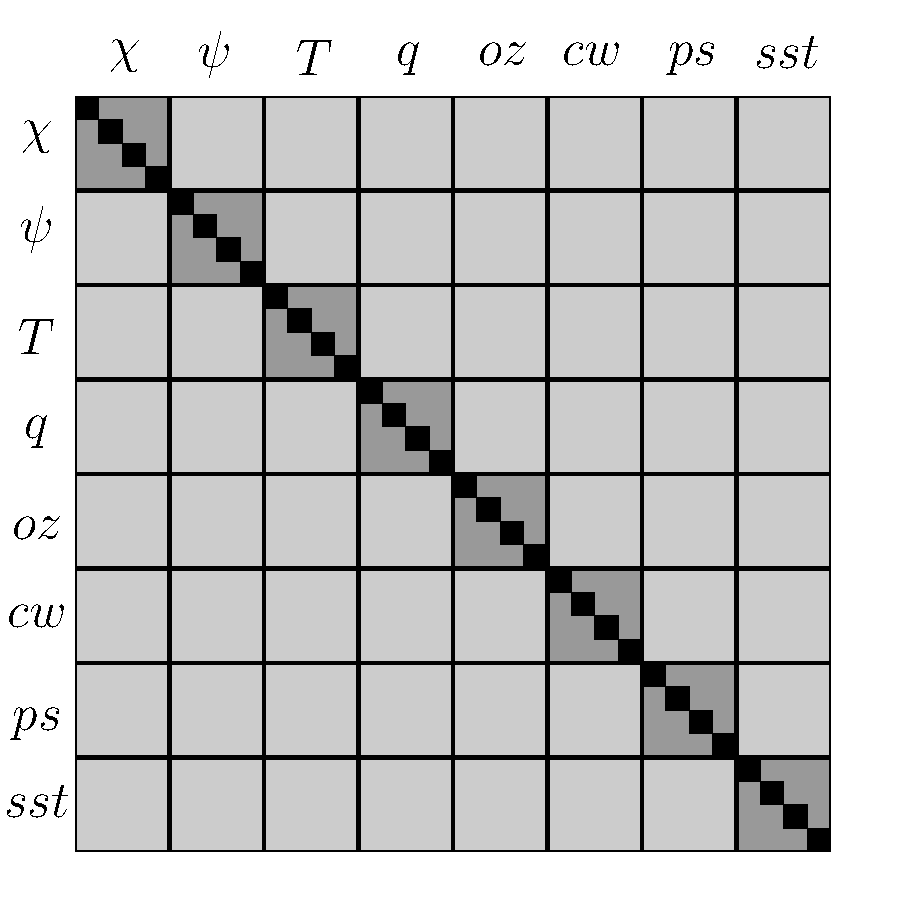
\includegraphics[scale=0.5]{./figs/cap3/matriz_B-new.pdf} 
\end{center}
 \vspace{2mm}
\legenda{No caso do GSI, as variáveis de estado analisadas são representadas: na diagonal principal os quadrados pretos representam as variâncias de cada variável; nos quadrados em cinza escuro, estão representados os elementos de autocovariância e em cinza claro, os elementos de covariância multivariados.}
\label{fig:1}
\FONTE{Adaptado de \citeonline{petrie/2012}}
\end{figure}

Para o cálculo da matriz de covariâncias do sistema GSI a partir do modelo de circulação geral do CPTEC, foram feitos dois testes. O primeiro teste considerou os pares de previsões de 48 e 24 horas que já estavam preparados na resolução TQ0299L064 (experimento denominado ``TAG'' - este experimento não faz parte do escopo deste trabalho) e extraídos do ciclo de assimilação de dados do sistema G3DVAR (versão 1.1.3) utilizando o modelo MCGAv4. O segundo teste considerou os pares de 48 e 24 horas do modelo BAMv0 na resolução TQ0062L028. Neste segundo teste, os pares de previsões foram obtidos a partir da realização do modelo BAMv0 usando as análises do NCEP. As justificativas para que o segundo teste tenha sido feito a com as análises do NCEP, são as seguintes: 1) foram encontradas inconsistências na representação das quantidades $oz$ e $cw$ na matriz de covariâncias quando esta foi calculada com base no MCGAv4; 2) embora seja possível calcular uma matriz de covariâncias para uma resolução menor do que a dos pares de entrada, estes pares não apresentaram valores consistentes de $oz$ e $cw$, fato este que não foi amenizado com a troca de resolução; 3) o problema com as quantidades $oz$ e $cw$ foi temporariamente resolvido utilizando-se as quantidades de $oz$ e $cw$ da matriz de covariâncias do NCEP, porém os primeiros testes do sistema híbrido 3DVar na resolução TQ0299L064 foram desencorajadores devido ao elevado custo computacional (e.g., dificuldades em alocar os recursos necessários para a realização dos membros do conjunto em tempo próximo do operacional); 4) não havia pares de previsões de 48 e 24 horas disponíveis para o MCGAv4 na resolução TQ0062L028 e portanto optou-se por testar uma versão mais recente do modelo de circulação geral do CPTEC (neste caso o modelo BAMv0) na tentativa de se sanar o problema com a representação de $oz$ e $cw$ (sem a necessidade de se copiar estas quantidades da matriz do NCEP) e facilitar a realização do sistema híbrido 3DVar. 

A matriz de covariâncias resultante do segundo teste foi então escolhida para a realização dos experimentos com o sistema híbrido 3DVar (cujos resultados são apresentados no Capítulo \ref{cap:resultados}). Nesta seção, portanto, são apresentadas as características principais das matrizes de covariâncias calculadas (nos dois testes mencionados), pois a matriz de covariâncias estática faz parte da metodologia aplicada ao longo deste trabalho.

O cálculo da matriz de covariâncias na resolução TQ0299L064 com os pares de previsões do modelo MCGAv4, foi feito com 1460 pares de previsões de 48 e 24 horas distribuídos ao longo de 1 ano (2013) no formato espectral. Os pares de previsões foram organizados na forma a seguir (válido também para a matriz de covariâncias do teste com o BAMv0): considerando-se o dia 2014010100, o primeiro par de previsões válido foi gerado com as análises dos dias 2013123100 (válido para uma previsão de 24 horas) e 2013123000 (válido para  uma previsão de 48 horas).

O algoritmo para o cálculo da matriz de covariâncias, cumpre as seguintes etapas:

\begin{enumerate}
    \item Leitura e organização dos pares de previsões de 48 e 24 horas;
	\item Remoção de viés (em toda a coluna vertical);
	\item Cálculo das matrizes de balanço que permitirão as transformações entre função de corrente ($\psi$) e as componentes desbalanceadas de velocidade potencial ($\chi$), pressão em superfície ($p$) e temperatura ($T$);
	\item Cálculo das variâncias dos erros de cada uma das variáveis de controle ($\psi$, $\chi$, $q$, $oz$, $cw$, $p$);
	\item Cálculo dos comprimentos de correlação verticais (em unidades inversas em ponto de grade);
	\item Cálculo dos comprimentos de correlação horizontais (em km).      
\end{enumerate}

No caso da matriz de covariâncias do MCGAv0 (na resolução TQ0299L064), nas etapas d), e) e f), as quantidades $oz$ e $cw$ foram posteriormente substituídas pelas quantidades correspondentes contidas na matriz de covariâncias do NCEP.

\section{Características Principais e Diagnósticos}

Nesta seção são apresentadas as características principais da matriz de covariâncias calculada no teste com o MCGAv4 (mencionado na seção anterior). As estruturas da matriz de covariâncias são apresentadas em termos de suas amplitudes. Como foram utilizados todos os pares de previsões de 48 e 24 horas disponíveis para o ano de 2013 na resolução TQ0299L028, foram calculadas também versões da matriz de covariâncias exclusivas para cada um dos horários sinóticos padrão (i.e., 00, 06, 12 e 18Z). Logo, uma comparação é feita entre estas versões da matriz de covariâncias do CPTEC com as versões completas das matrizes de covariâncias do CPTEC e NCEP. O objetivo destas comparações é caracterizar de forma quantitativa e qualitativa as matrizes calculadas. 

\subsection*{Características Principais da Matriz de Covariâncias do MCGA v4.x}

A matriz de covariâncias do GSI possui as seguintes estruturas: amplitudes (representadas por variâncias e desvios-padrão), distâncias (representadas pelos comprimentos de escalas horizontal e vertical) e matrizes de projeção de balanço. A matriz de covariâncias utilizada pelo CPTEC (3DVar) varia apenas nas latitudes e na vertical. As variáveis de estado do GSI são a função de corrente, a velocidade potencial desbalanceada, a temperatura virtual desbalanceada, a pressão em superfície, a pseudo umidade relativa (ou umidade relativa normalizada), a razão de mistura de ozônio e a razão de mistura de condensação em nuvens. Para cada uma destas variáveis são definidas amplitudes e as distâncias. As variáveis velocidade potencial, temperatura e pressão em superfície, possuem matrizes de projeção que são responsáveis por projetar o incremento da função de corrente no perfil da parte balanceada do incremento de cada uma destas quantidades. Para a velocidade potencial, uma matriz de correlação é utilizada para contabilizar a correlação positiva entre divergência e vorticidade.

Para se verificar a qualidade das amplitudes calculadas a partir dos pares de previsões do modelo de circulação geral MCGAv4 na resolução TQ0299L064, foram calculadas as amplitudes para os horários sinóticos padrão (00, 06, 12 e 18Z) e para todos os horários juntos (``AllZ''), para o período de 1 ano. Para este período de tempo, foi utilizado um total de 1460 pares (contabilizando todos os horários sinóticos) e 365 pares de previsões para as matrizes exclusivas de cada horário sinótico. Para comparação, foi utilizada a matriz de covariâncias do NCEP, calculada utilizando-se os pares de previsão do modelo GFS. Segundo \citeonline{wuetal/2002}, esta matriz foi calculada utilizando-se 49 pares de previsões, distribuídos ao longo de 1 ano. Em todos os casos, as comparações são feitas na grade de dimensões 768x386x64 (lon x lat x lev).

\begin{figure}[H]
    \caption{Distribuição das amplitudes calculadas para a matriz $\mathbf{B}$ na resolução TQ0299L064.}
    \vspace{2mm}
    \begin{center}
        \subfigure[$\mathbf{B}$ NCEP (ALLZ), $\psi$]{
          \label{fig:bncep_allz_psi}
          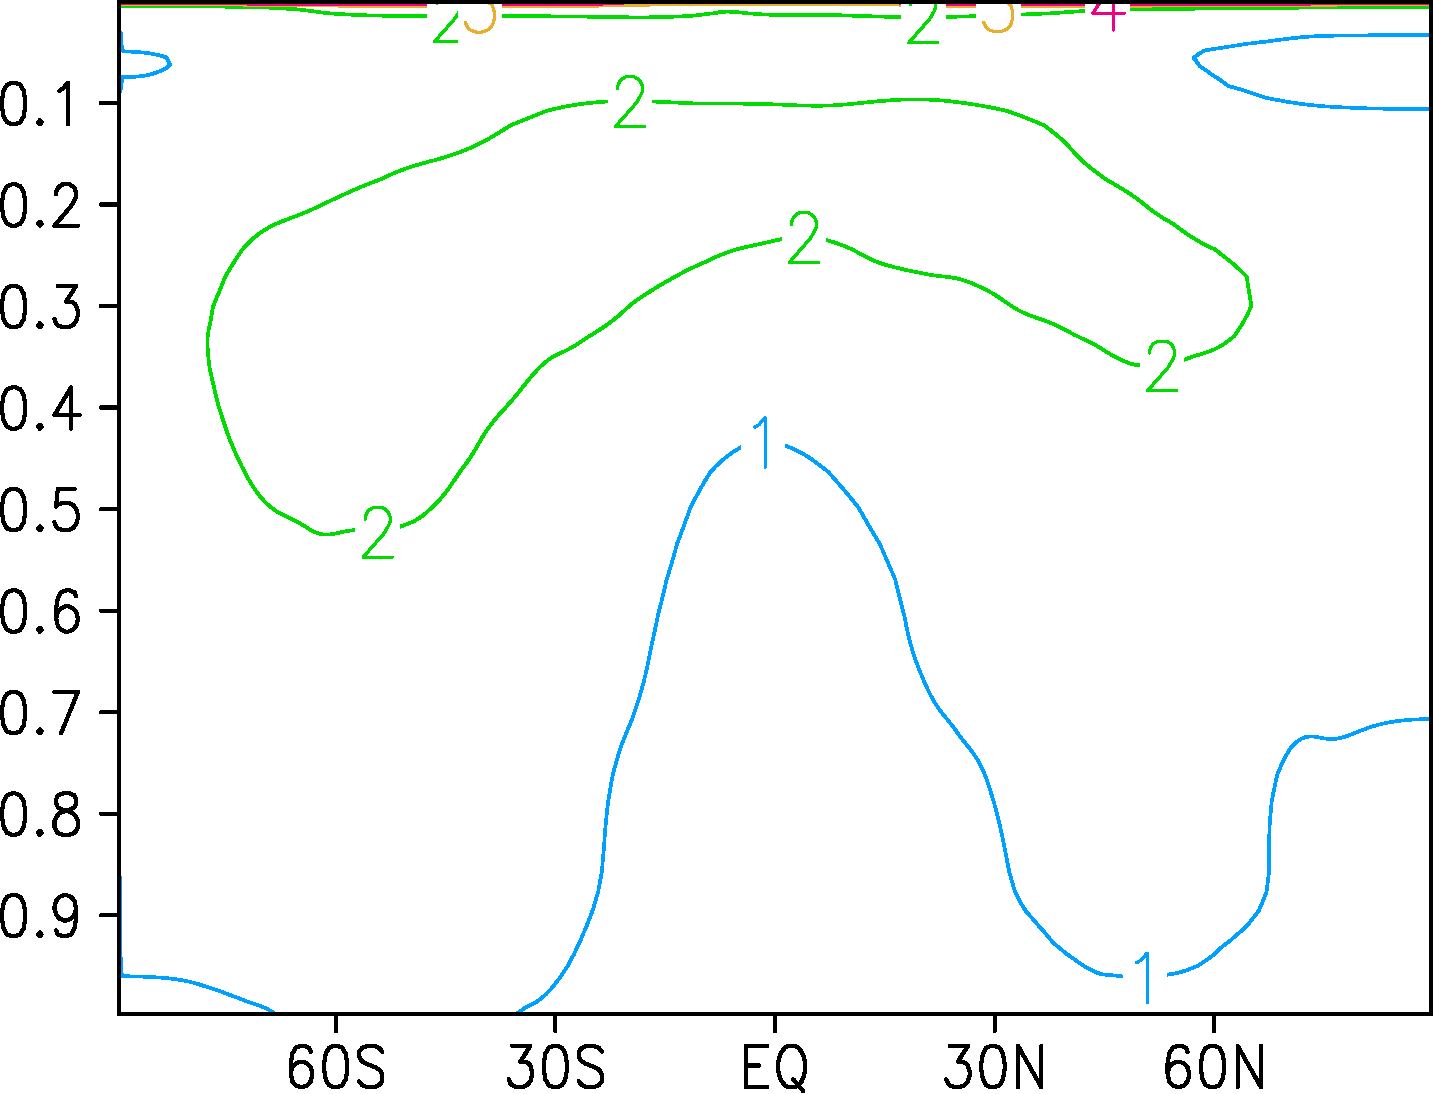
\includegraphics[width=0.3\textwidth,angle=0]{./figs/cap3/amplitudes_novas/amplitudes-NCEP_sf-crop-rotated270.pdf}
        }
        \subfigure[$\mathbf{B}$ CPTEC (00Z), $\psi$]{
          \label{fig:bcptec_00z_psi}
          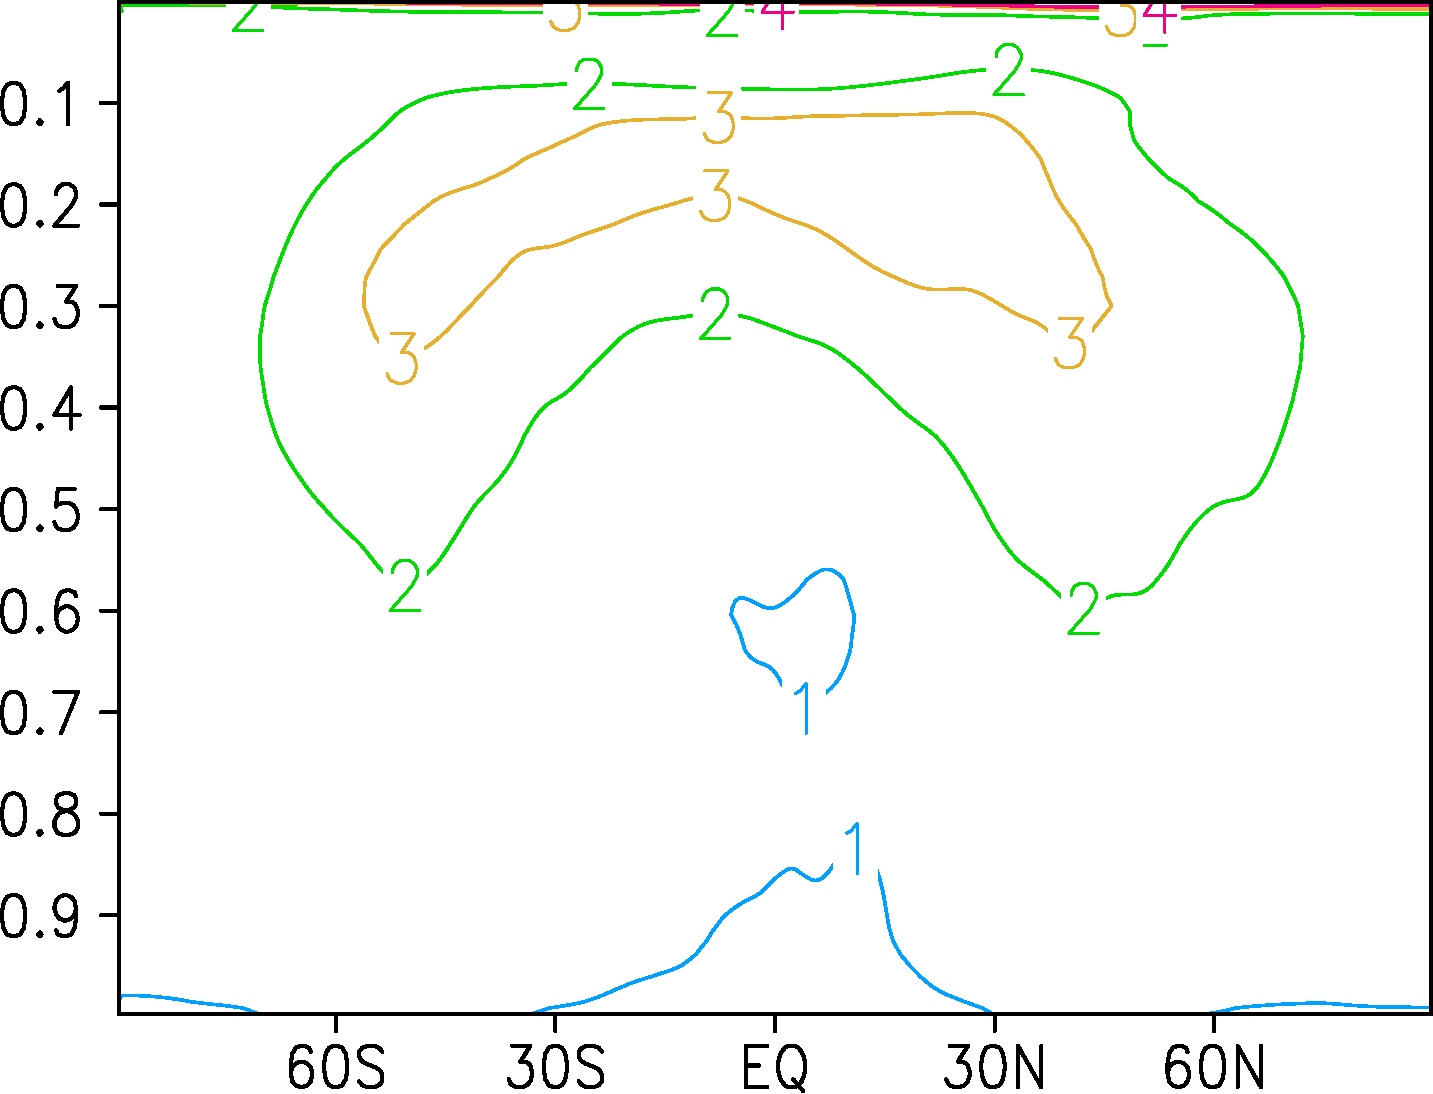
\includegraphics[width=0.3\textwidth,angle=0]{./figs/cap3/amplitudes_novas/amplitudes-B00Z_sf-crop-rotated270.pdf}          
        } 
        \subfigure[$\mathbf{B}$ CPTEC (06Z), $\psi$]{
          \label{fig:bcptec_06z_psi}
          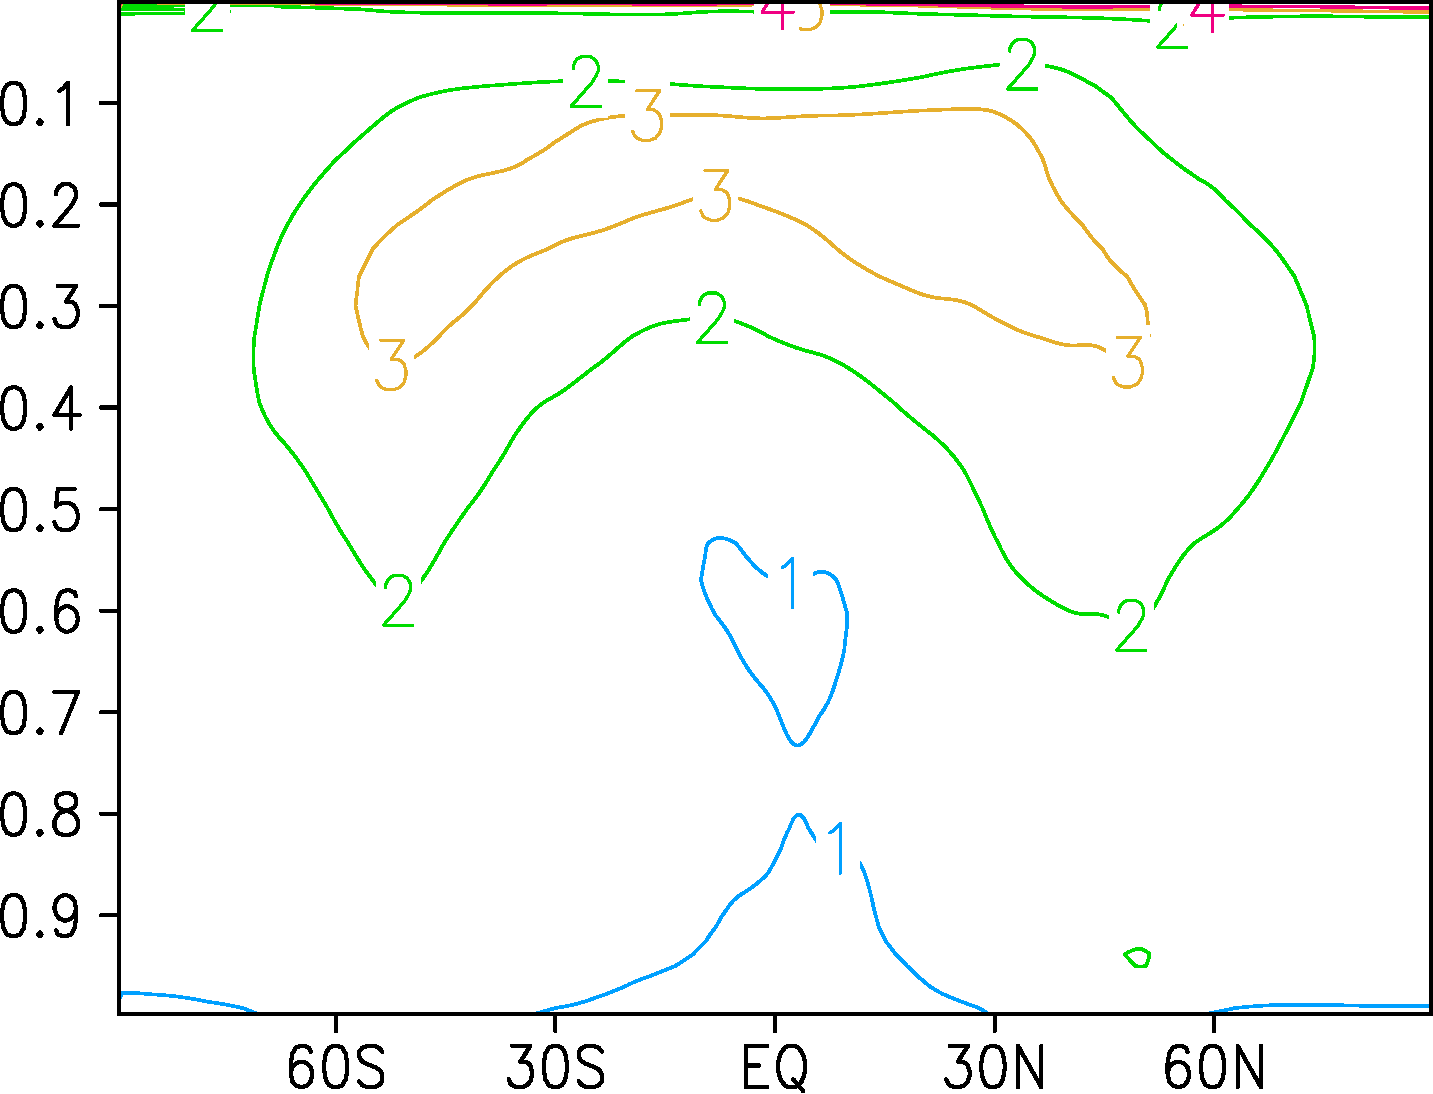
\includegraphics[width=0.3\textwidth,angle=0]{./figs/cap3/amplitudes_novas/amplitudes-B06Z_sf-crop-rotated270.pdf}
        } \\
        \subfigure[$\mathbf{B}$ CPTEC (ALLZ), $\psi$]{
          \label{fig:bcptec_allz_psi}
          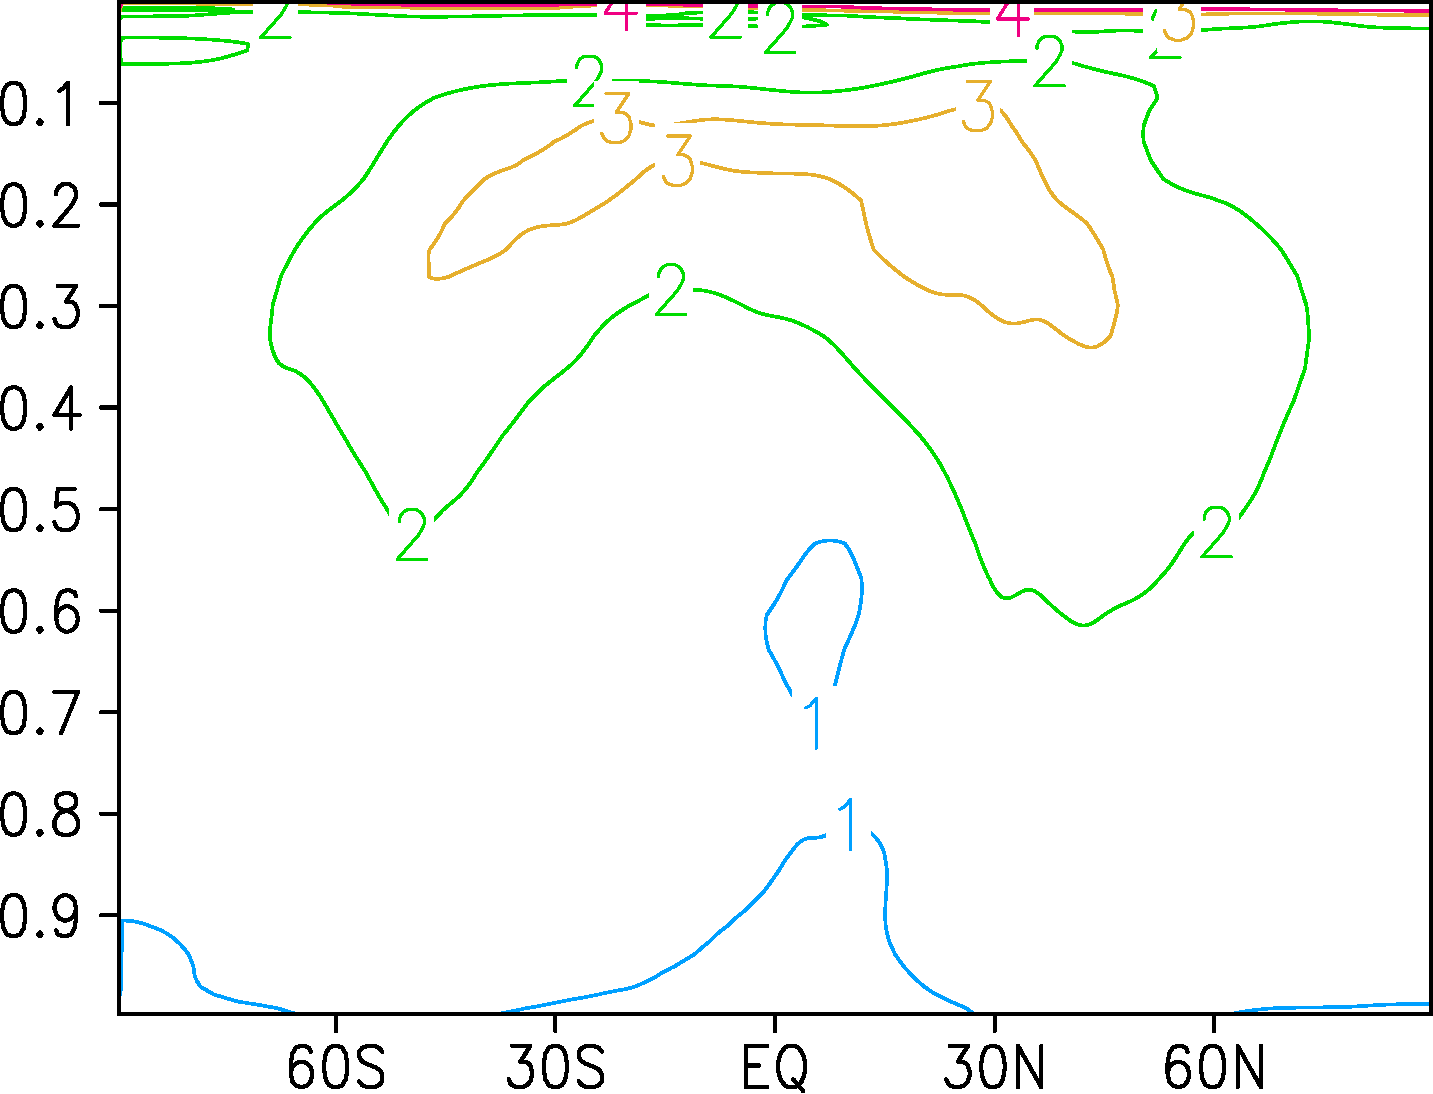
\includegraphics[width=0.3\textwidth,angle=0]{./figs/cap3/amplitudes_novas/amplitudes-BAllZ_sf-crop-rotated270.pdf}
        }   
        \subfigure[$\mathbf{B}$ CPTEC (12Z), $\psi$]{
          \label{fig:bcptec_12z_psi}
          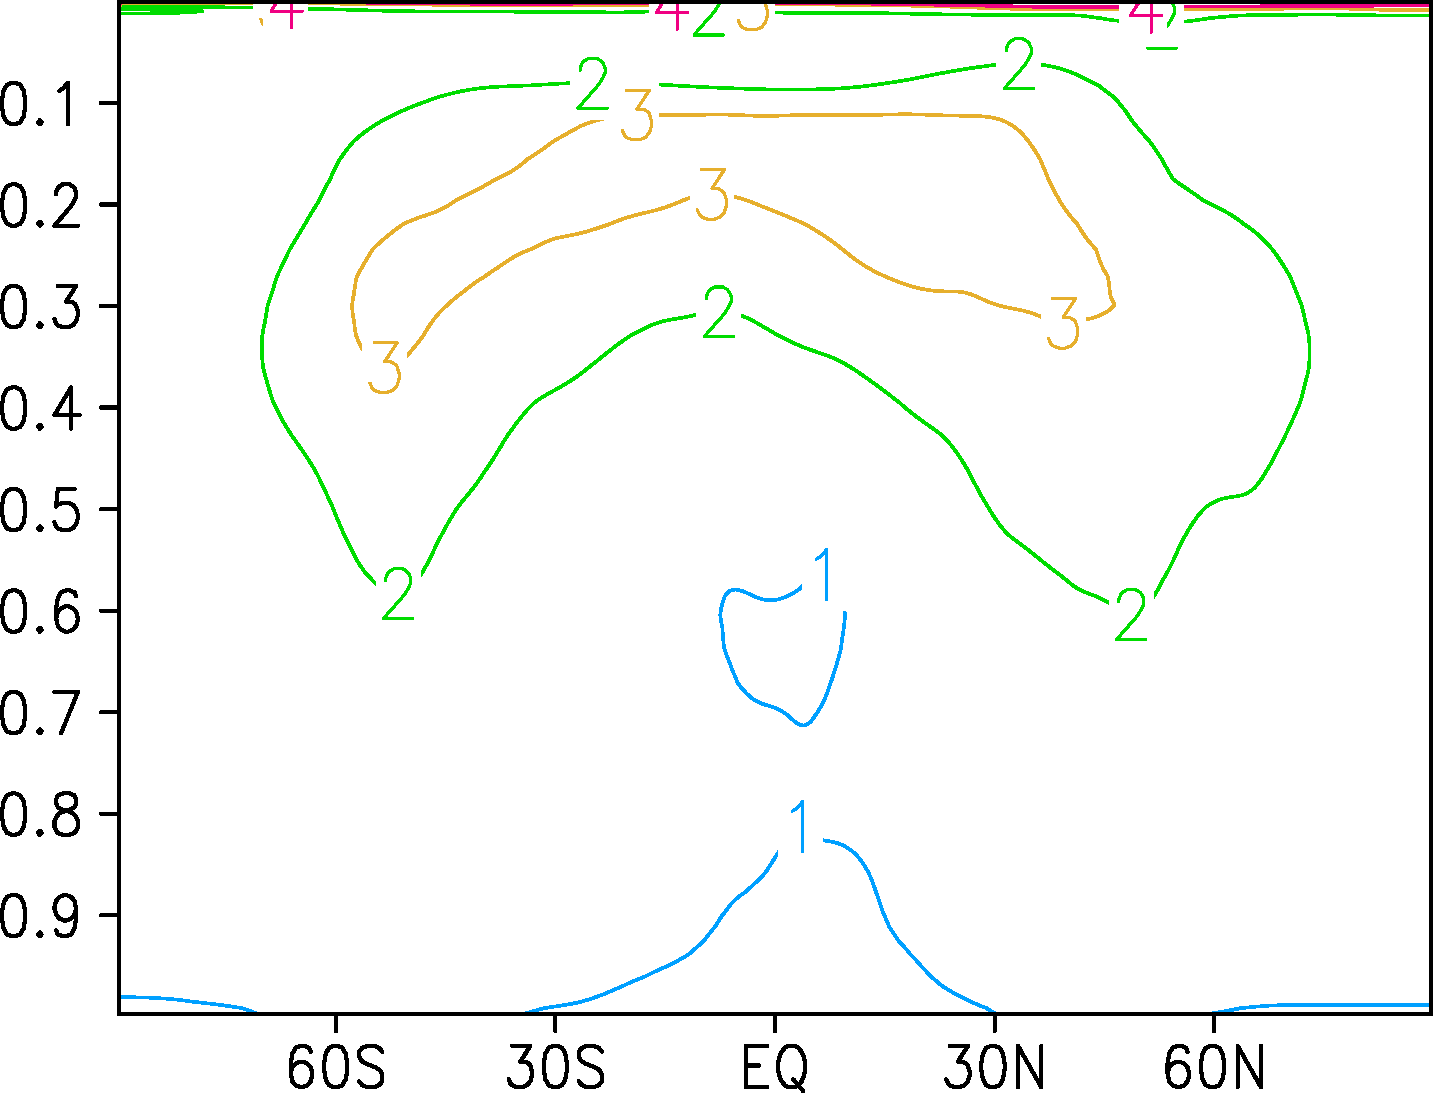
\includegraphics[width=0.3\textwidth,angle=0]{./figs/cap3/amplitudes_novas/amplitudes-B12Z_sf-crop-rotated270.pdf}
        }    
        \subfigure[$\mathbf{B}$ CPTEC (18Z), $\psi$]{
          \label{fig:bcptec_18z_psi}
          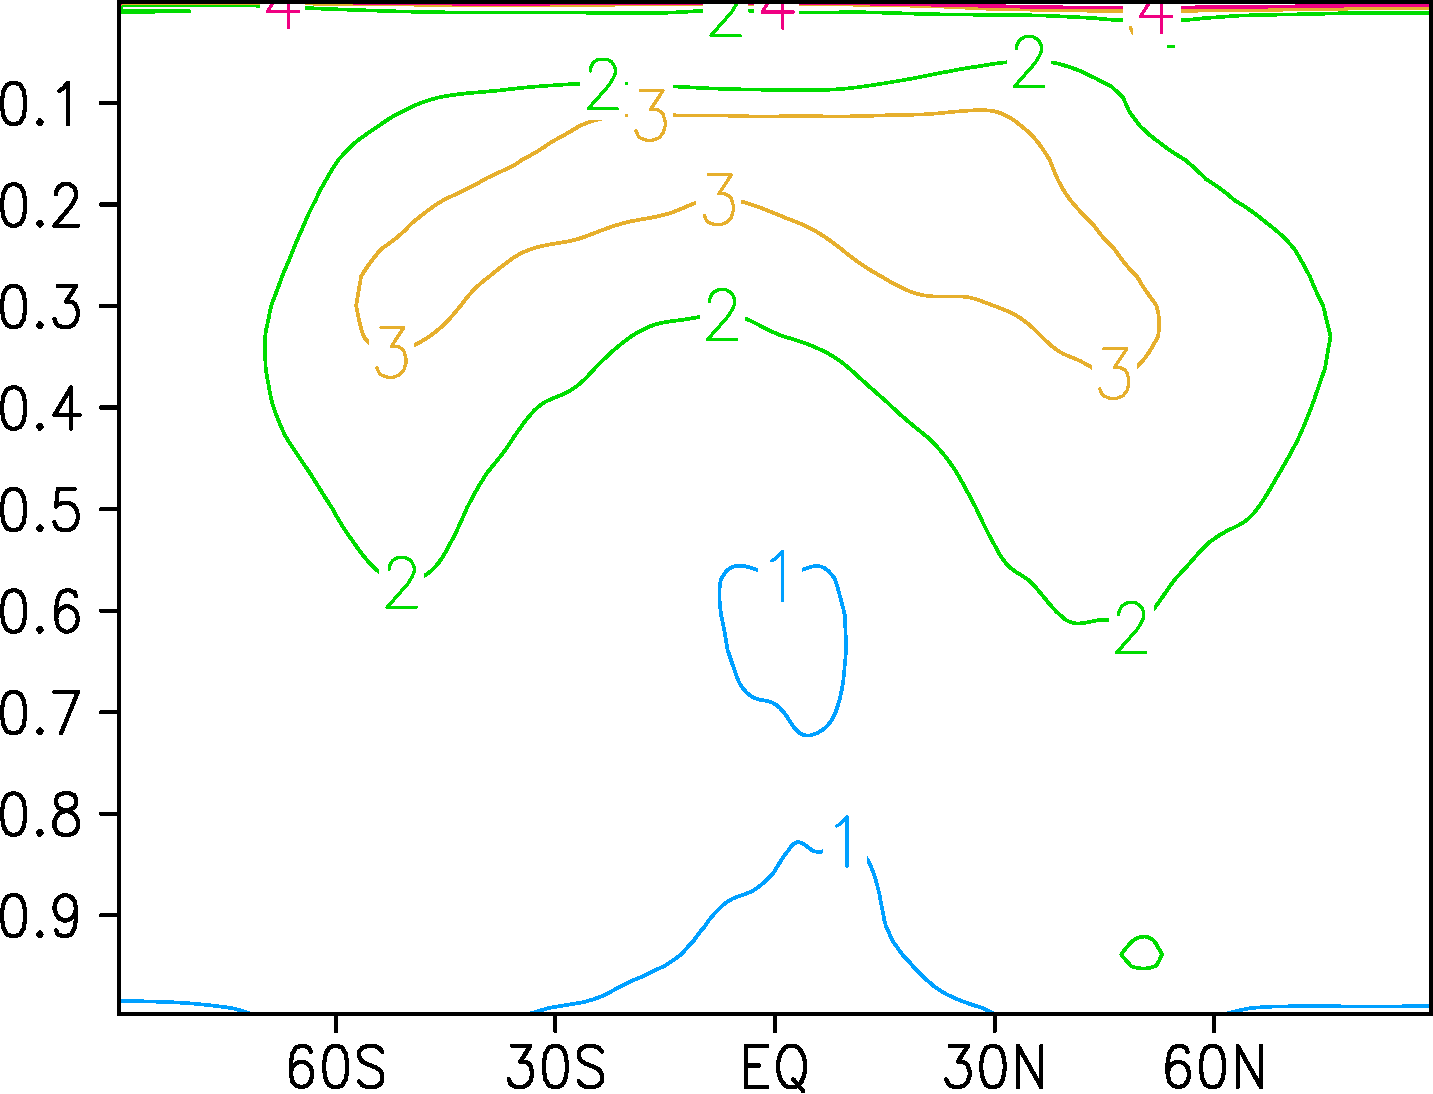
\includegraphics[width=0.3\textwidth,angle=0]{./figs/cap3/amplitudes_novas/amplitudes-B18Z_sf-crop-rotated270.pdf}
        }   
    \end{center}
    \vspace{2mm}
    \legenda{Amplitudes da função de corrente ($\psi$, x $10^{-6}$) ao longo das latitudes e níveis sigma, calculadas utilizando-se o método NMC para todos os horários sinóticos e todos os horários separados. A comparação é feita com o NCEP.}
    \label{fig:B_mcgav4_psi}
    \FONTE{Produção do autor.}
\end{figure}

A Figura \ref{fig:B_mcgav4_psi} mostra a distribuição vertical e latitudinal das amplitudes (variâncias/desvios-padrão) da função de corrente provenientes da matriz de covariâncias do NCEP e do CPTEC. Comparando-se as Figuras \ref{fig:bncep_allz_psi} e \ref{fig:bcptec_allz_psi} (as duas matrizes contendo os pares de previsões de todos os horários sinóticos padrão), observa-se que a amplitude da função de corrente da matriz do CPTEC é mais concentrada, sendo confinada entre os níveis 0.3 a 0.1 sigma (aproximadamente entre 307.2 e 102.4 hPa). As isolinhas de amplitude da função de corrente da matriz do CPTEC, mostram valores maiores nesta região (3x$10^{-6}$) enquanto que a matriz do NCEP apresenta valores menores na mesma região (2x$10^{-6}$), mas espalhado entre os níveis sigma 0.5 e 0.1 (512 e 102.4). Além disso, pode-se observar também a distribuição da amplitude ao longo das latitudes (90N e 90S); nos trópicos ela é menor, apresentando um padrão em forma de ``sino'' (o qual pode ser melhor observado nas demais matrizes, calculadas com os pares de previsões dos horários sinóticos em separado) e maior nos polos.

Esta distribuição da amplitude (variância) da função de corrente para a matriz do CPTEC calculada utilizando-se todos os pares de previsão, não é exatamente semelhante a matriz correspondente do NCEP e esta comparação mostra que, de forma geral, a amplitude da função de corrente no Hemisfério Norte é maior na matriz do CPTEC (o valor em sí é maior e a faixa de latitudes envolvida também), enquanto que esta mesma amplitude é menor no Hemisfério Sul, como representado na matriz de covariâncias do CPTEC. Isto pode estar relacionado a forma como os pares de previsão foram gerados: para o cálculo da matriz de covariâncias do CPTEC, foram utilizados pares de previsões de 48 e 24 horas provenientes do ciclo de assimilação de dados do CPTEC, utilizando-se observações regionalizadas (além daquelas provenientes do \textit{Global Telecomunication System} - GTS). Consequentemente, a variância do erro sobre o Hemisfério Sul, sobretudo sobre a América do Sul (entre 0 e 60S) pode ser menor. Nas outras matrizes do CPTEC (calculadas com os pares exclusivos das 00, 06, 12 e 18Z), observa-se uma distribuição quase simétrica da amplitude da função de corrente, com valores mais próximos da matriz do NCEP, mas com a distribuição, mais localizada ao sul do continente sul-americano.

A Figura \ref{fig:B_mcgav4_chi} mostra a distribuição das amplitudes da velocidade potencial. Assim como para a Figura \ref{fig:B_mcgav4_psi}, as amplitudes calculadas para a velocidade potencial mostram que sobre a região tropical (entre 30S e 30N), a variância do erro na matriz do CPTEC é maior do que a representada pela matriz do NCEP, sobretudo entre os níveis mais baixos do modelo até o nível sigma 0.6 (614 hPa). Comparativamente, cada uma das demais matrizes do CPTEC (00, 06, 12 e 18Z) apresentam similaridades entre si (principalmente entre as matrizes das 00 e 12Z e 06 e 18Z - Figuras \ref{fig:bcptec_00z_chi} e \ref{fig:bcptec_12z_chi}; \ref{fig:bcptec_06z_chi} e \ref{fig:bcptec_18z_chi}, respectivamente).

\begin{figure}[H]
    \vspace{2mm}
    \caption{Idem Figura \ref{fig:B_mcgav4_psi}, para a velocidade potencial ($\chi$ x $10^{-6}$).}
    \begin{center}
        \subfigure[$\mathbf{B}$ NCEP (ALLZ), $\chi$]{
          \label{fig:bncep_allz_chi}
          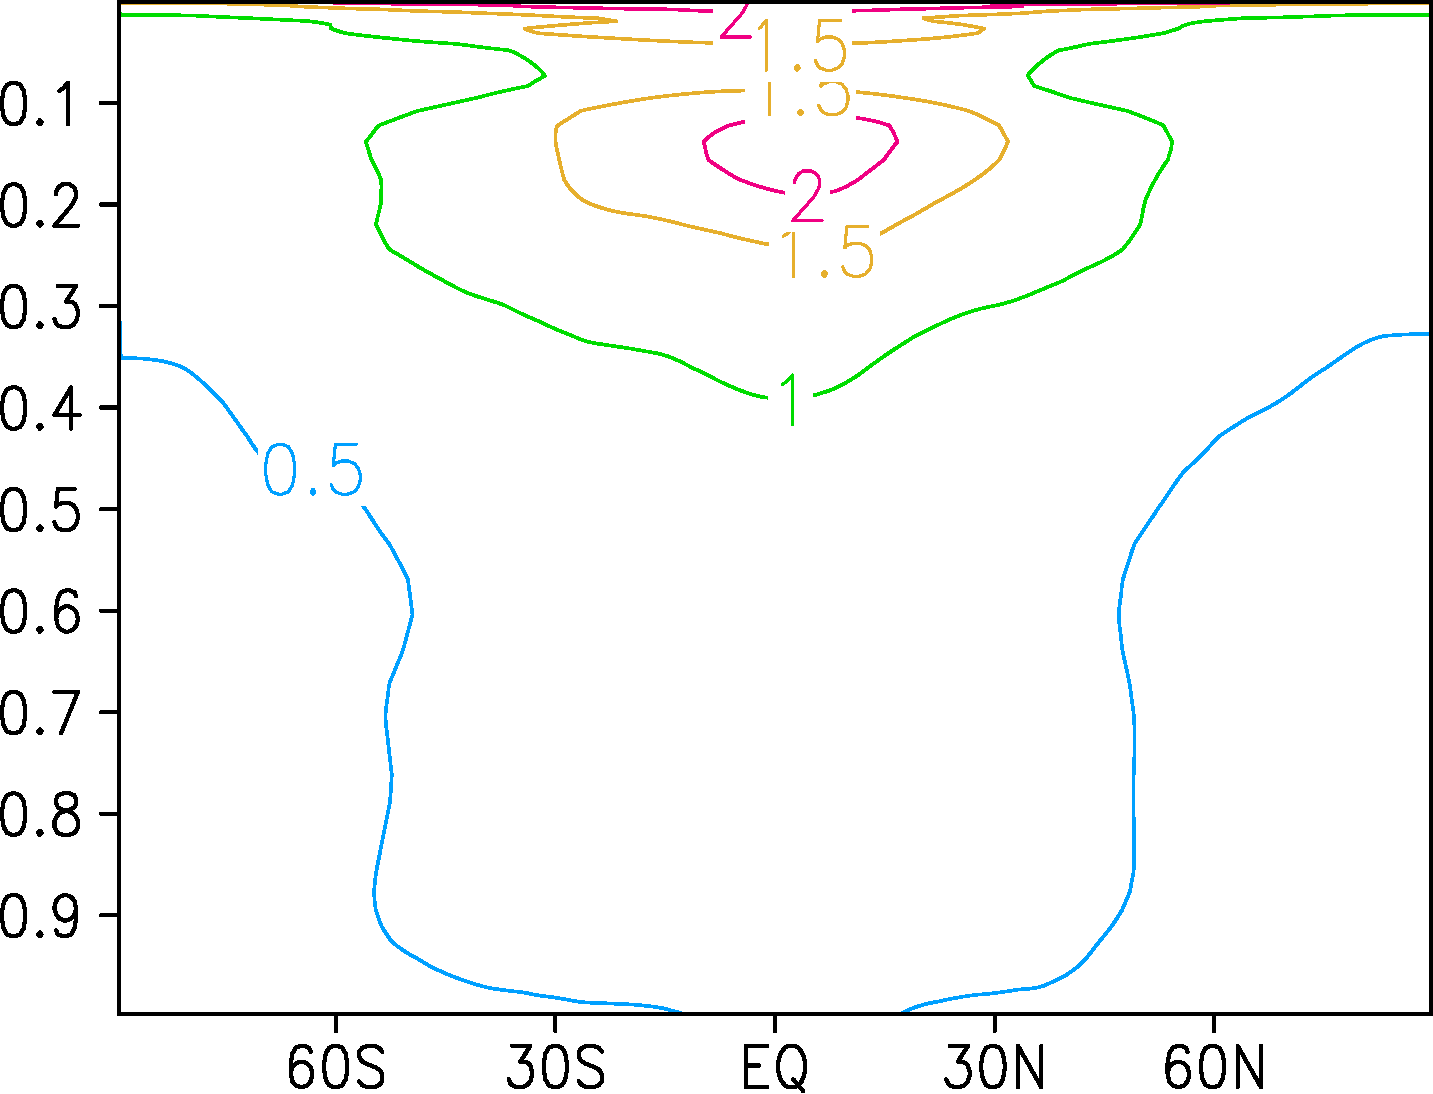
\includegraphics[width=0.3\textwidth,angle=0]{./figs/cap3/amplitudes_novas/amplitudes-NCEP_vp-crop-rotated270.pdf} 
        }
        \subfigure[$\mathbf{B}$ CPTEC (00Z), $\chi$]{
          \label{fig:bcptec_00z_chi}
          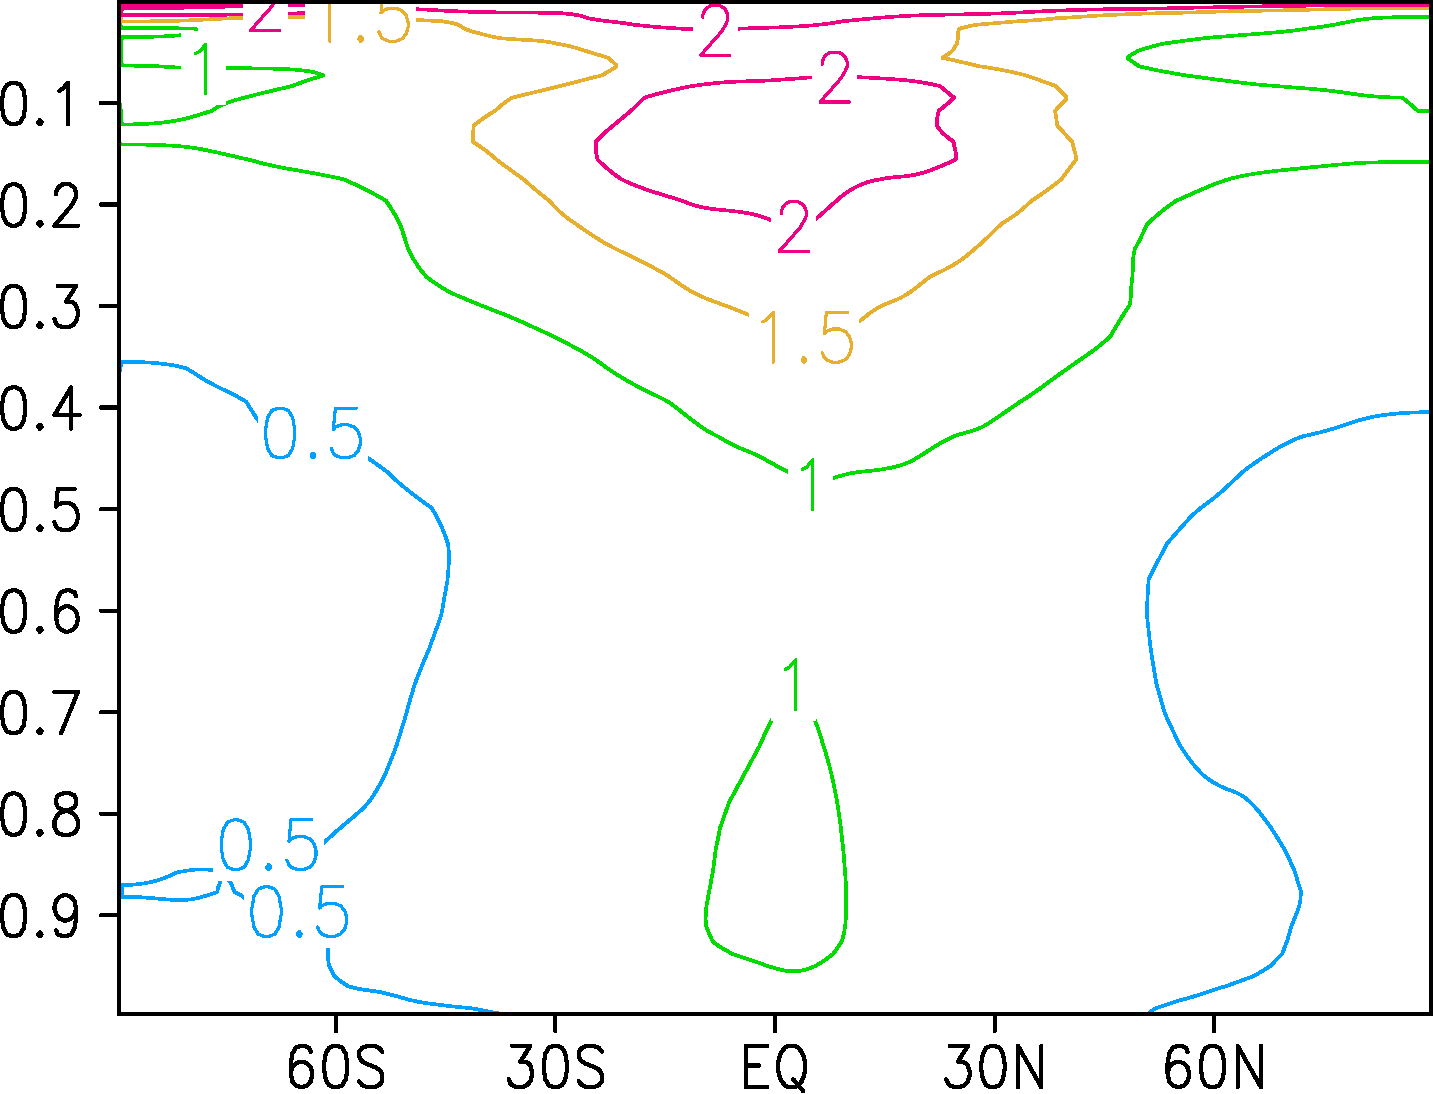
\includegraphics[width=0.3\textwidth,angle=0]{./figs/cap3/amplitudes_novas/amplitudes-B00Z_vp-crop-rotated270.pdf} 
        } 
        \subfigure[$\mathbf{B}$ CPTEC (06Z), $\chi$]{
          \label{fig:bcptec_06z_chi}
          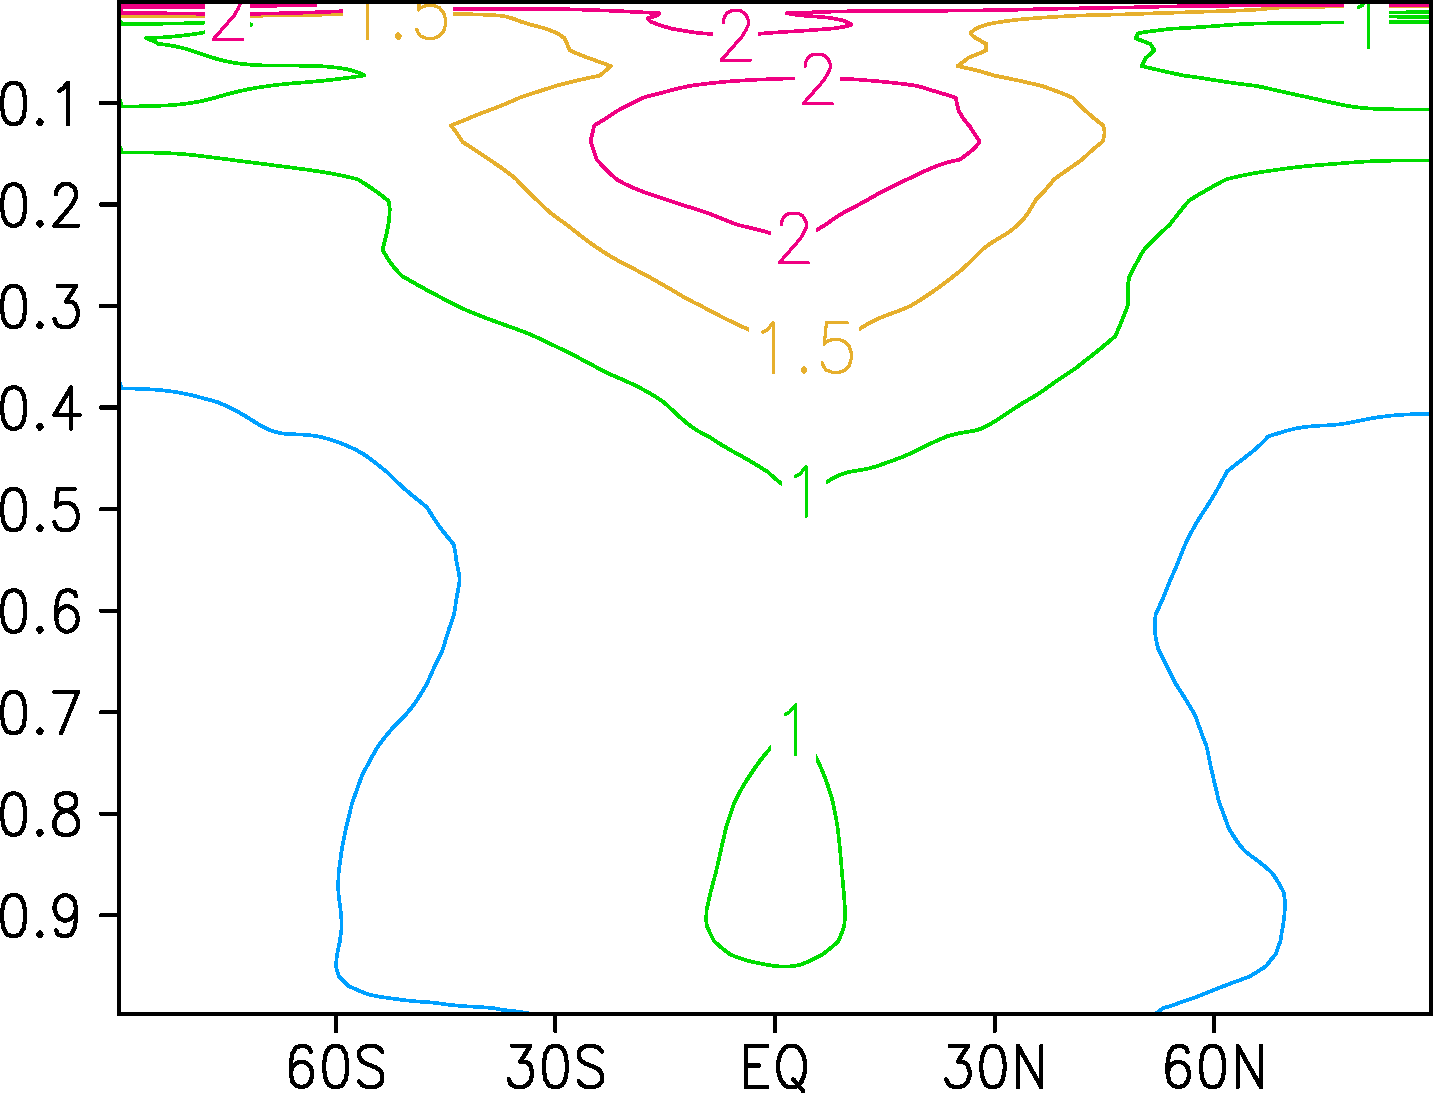
\includegraphics[width=0.3\textwidth,angle=0]{./figs/cap3/amplitudes_novas/amplitudes-B06Z_vp-crop-rotated270.pdf}
        } \\
        \subfigure[$\mathbf{B}$ CPTEC (ALLZ), $\chi$]{
          \label{fig:bcptec_allz_chi}
          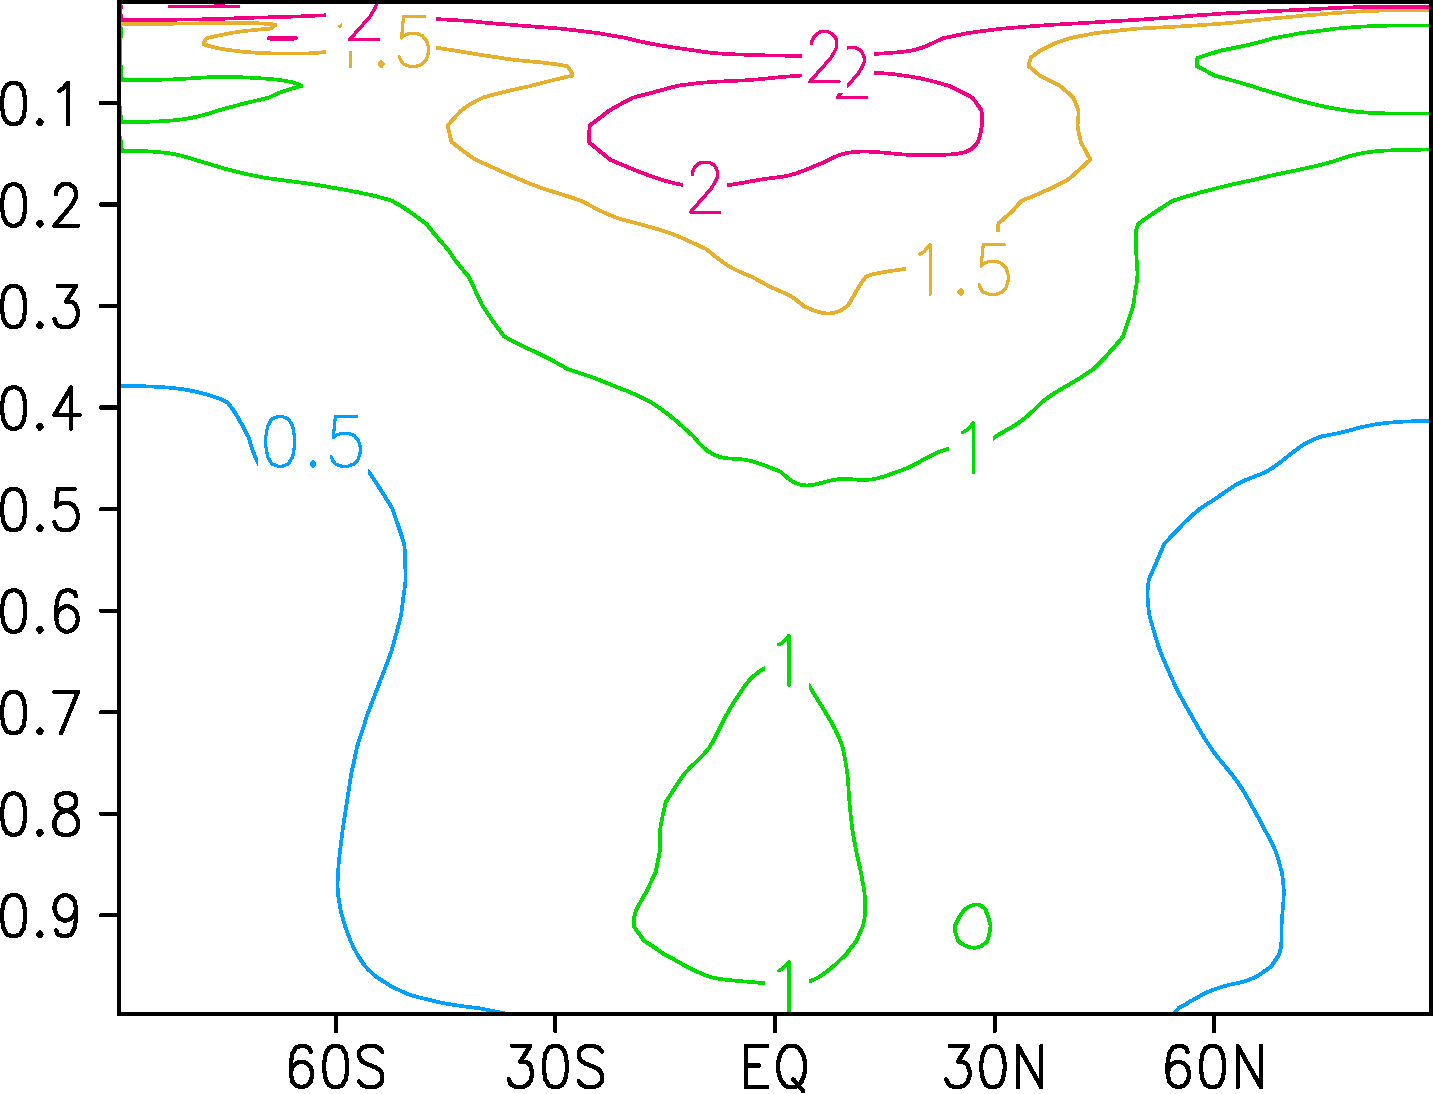
\includegraphics[width=0.3\textwidth,angle=0]{./figs/cap3/amplitudes_novas/amplitudes-BAllZ_vp-crop-rotated270.pdf}
        }   
        \subfigure[$\mathbf{B}$ CPTEC (12Z), $\chi$]{
          \label{fig:bcptec_12z_chi}
          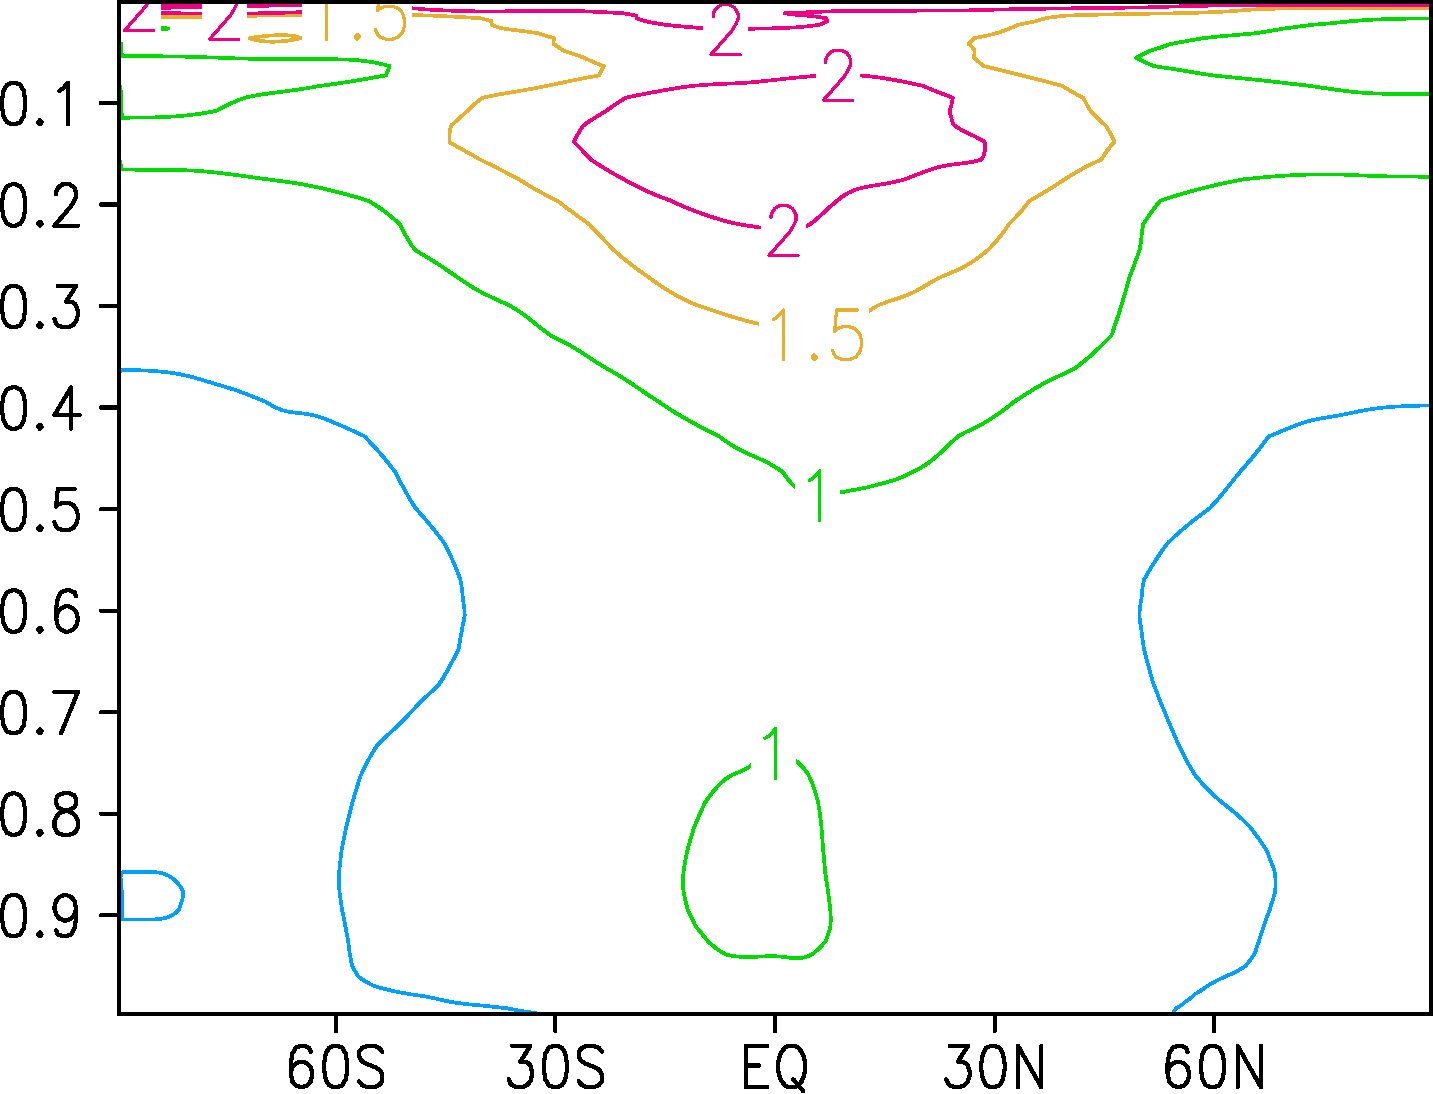
\includegraphics[width=0.3\textwidth,angle=0]{./figs/cap3/amplitudes_novas/amplitudes-B12Z_vp-crop-rotated270.pdf}
        }    
        \subfigure[$\mathbf{B}$ CPTEC (18Z), $\chi$]{
          \label{fig:bcptec_18z_chi}
          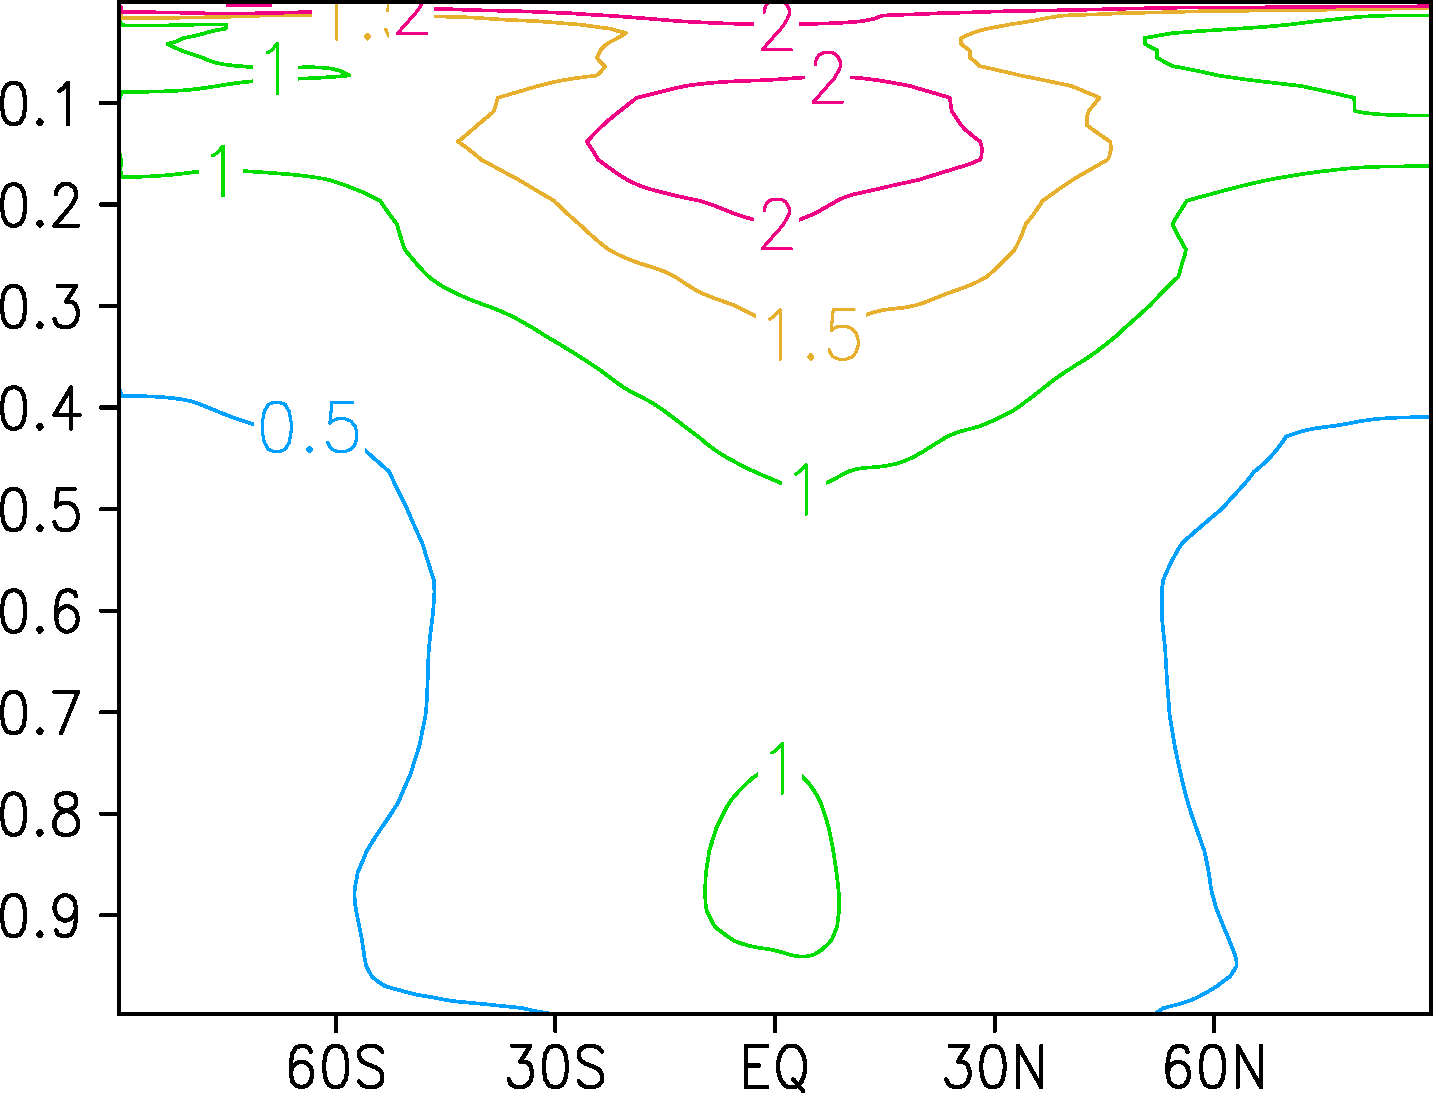
\includegraphics[width=0.3\textwidth,angle=0]{./figs/cap3/amplitudes_novas/amplitudes-B18Z_vp-crop-rotated270.pdf}
        }   
    \end{center}
  \vspace{2mm}
  \legenda{}
  \label{fig:B_mcgav4_chi}
  \FONTE{Produção do autor.}
\end{figure}

A Figura \ref{fig:B_mcgav4_T} a seguir, apresenta a distribuição das amplitudes da temperatura, sendo que estes valores na matriz do CPTEC completa (i.e., BAllZ - Figura \ref{fig:bcptec_00z_t}), onde a maior parte da variância encontra-se concentrada sobre o Hemisfério Norte, mais precisamente a partir de 30N (isolinha de 1 na Figura \ref{fig:bcptec_00z_t}); esta mesma isolinha na matriz do NCEP (Figura \ref{fig:bncep_allz_t}) está desenhada a partir de aproximadamente 45N. Em ambas as matrizes, esta amplitude é limitada as primeiras camadas do modelo (ie., entre a superfície e o nível sigma de 0.8 ou 819.2 hPa). Nas demais matrizes, observa-se um padrão semelhante em relação a distribuição das amplitudes, sendo que no Hemisfério Norte, estas alcançam os 819.2 hPa, enquanto que no Hemisfério Sul, não ultrapassam este nível.


\begin{figure}[H]
    \vspace{2mm}
    \caption{Idem Figura \ref{fig:B_mcgav4_psi}, para a temperatura ($T$).}
    \begin{center}
        \subfigure[$\mathbf{B}$ NCEP (ALLZ), $T$]{
          \label{fig:bncep_allz_t}
          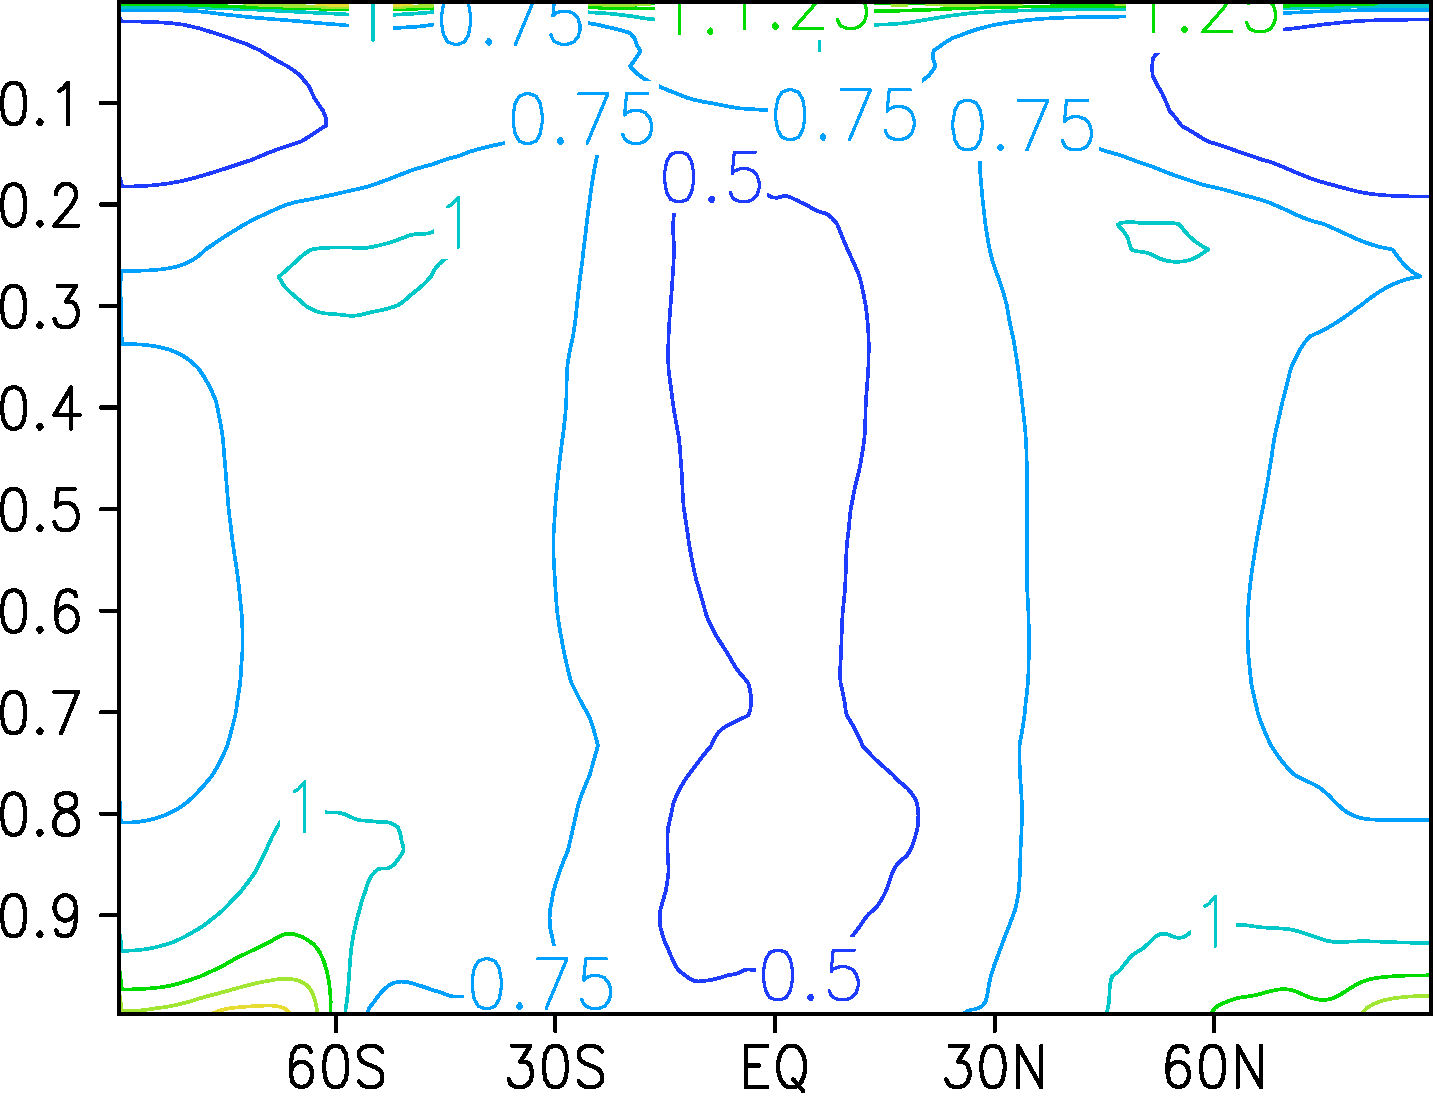
\includegraphics[width=0.3\textwidth,angle=0]{./figs/cap3/amplitudes_novas/amplitudes-NCEP_t-crop-rotated270.pdf} 
        }
        \subfigure[$\mathbf{B}$ CPTEC (00Z), $T$]{
          \label{fig:bcptec_00z_t}
          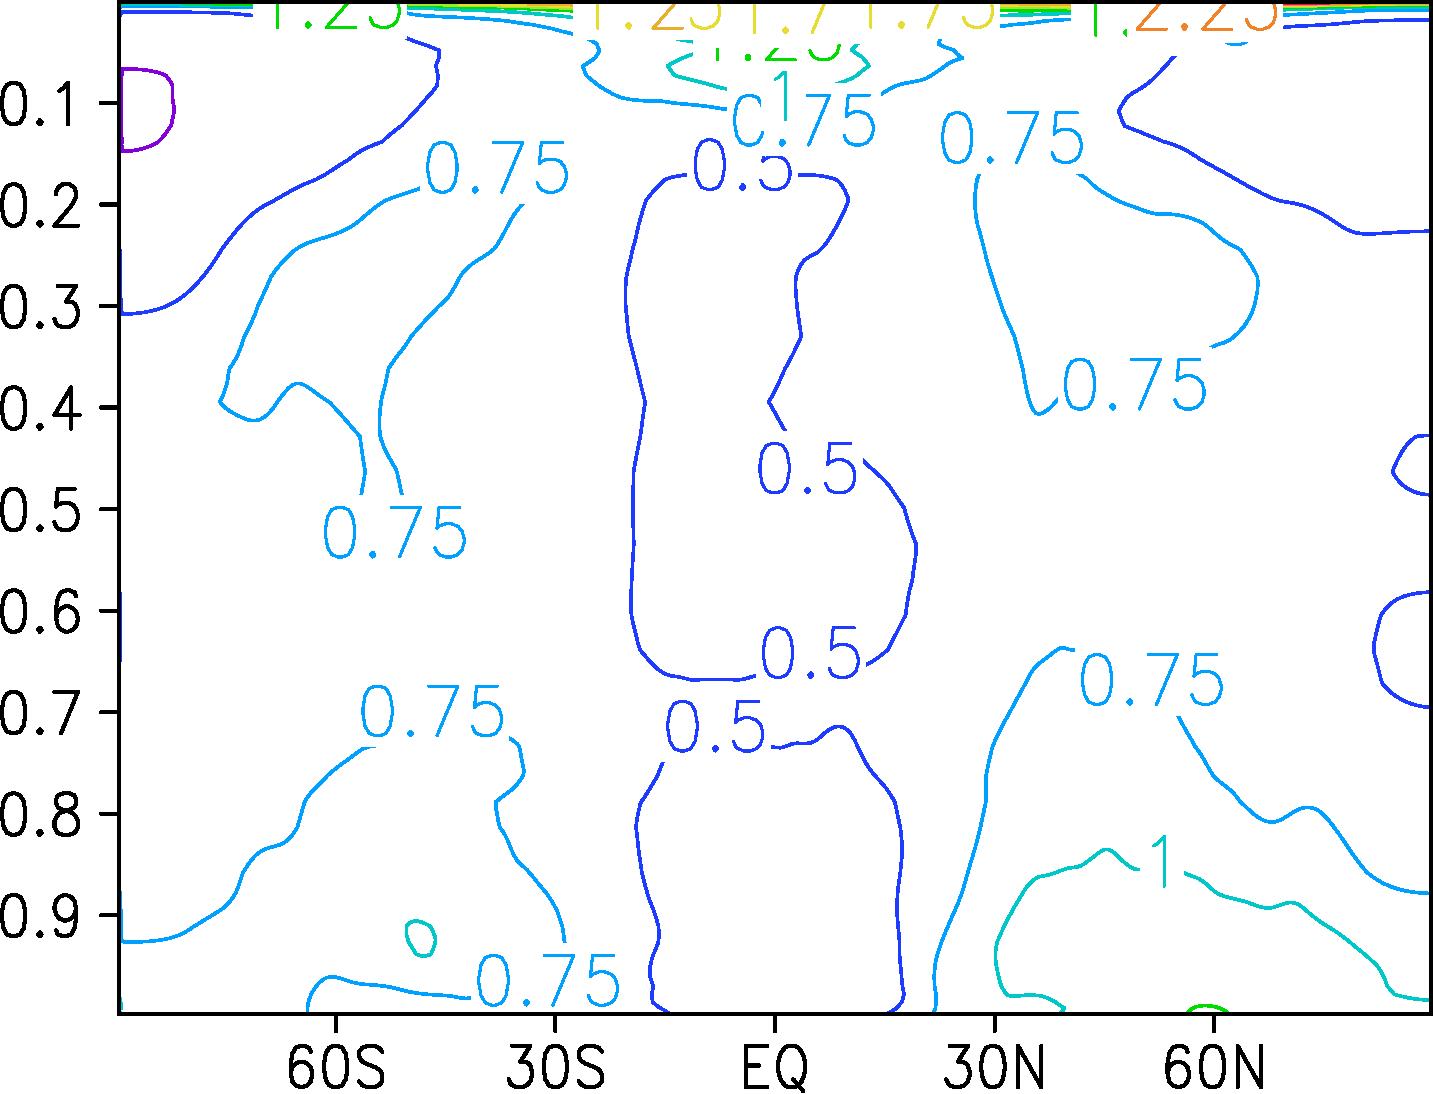
\includegraphics[width=0.3\textwidth,angle=0]{./figs/cap3/amplitudes_novas/amplitudes-B00Z_t-crop-rotated270.pdf}
        } 
        \subfigure[$\mathbf{B}$ CPTEC (06Z), $T$]{
          \label{fig:bcptec_06z_t}
          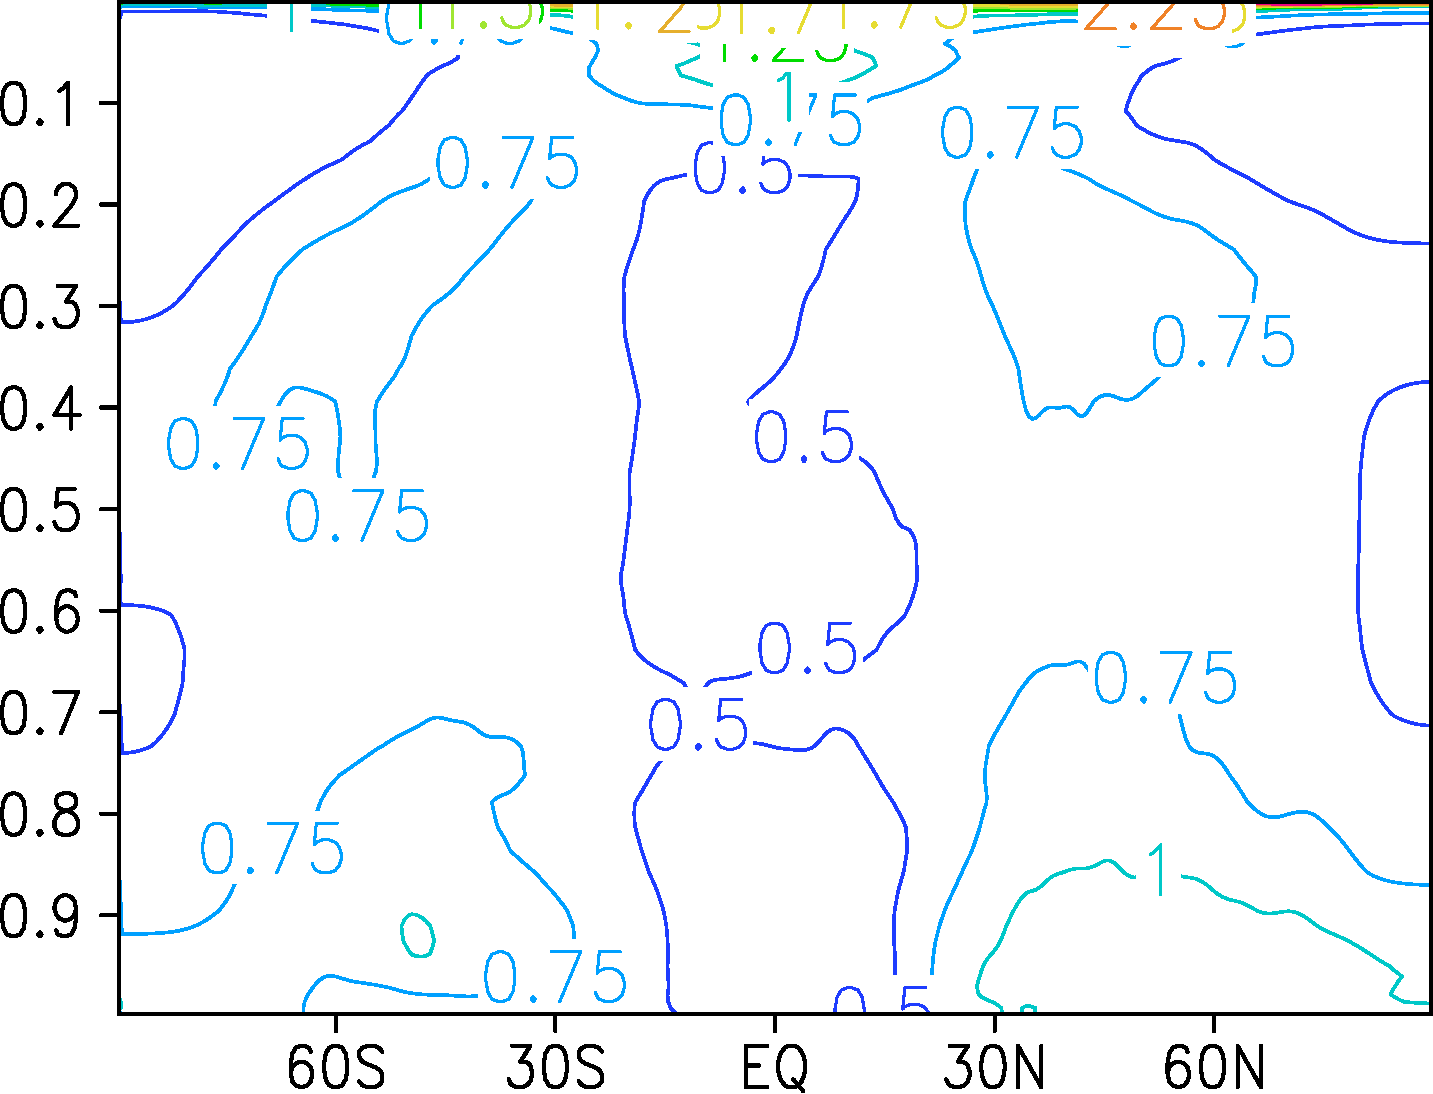
\includegraphics[width=0.3\textwidth,angle=0]{./figs/cap3/amplitudes_novas/amplitudes-B06Z_t-crop-rotated270.pdf}
        } \\
        \subfigure[$\mathbf{B}$ CPTEC (ALLZ), $T$]{
          \label{fig:bcptec_allz_t}
          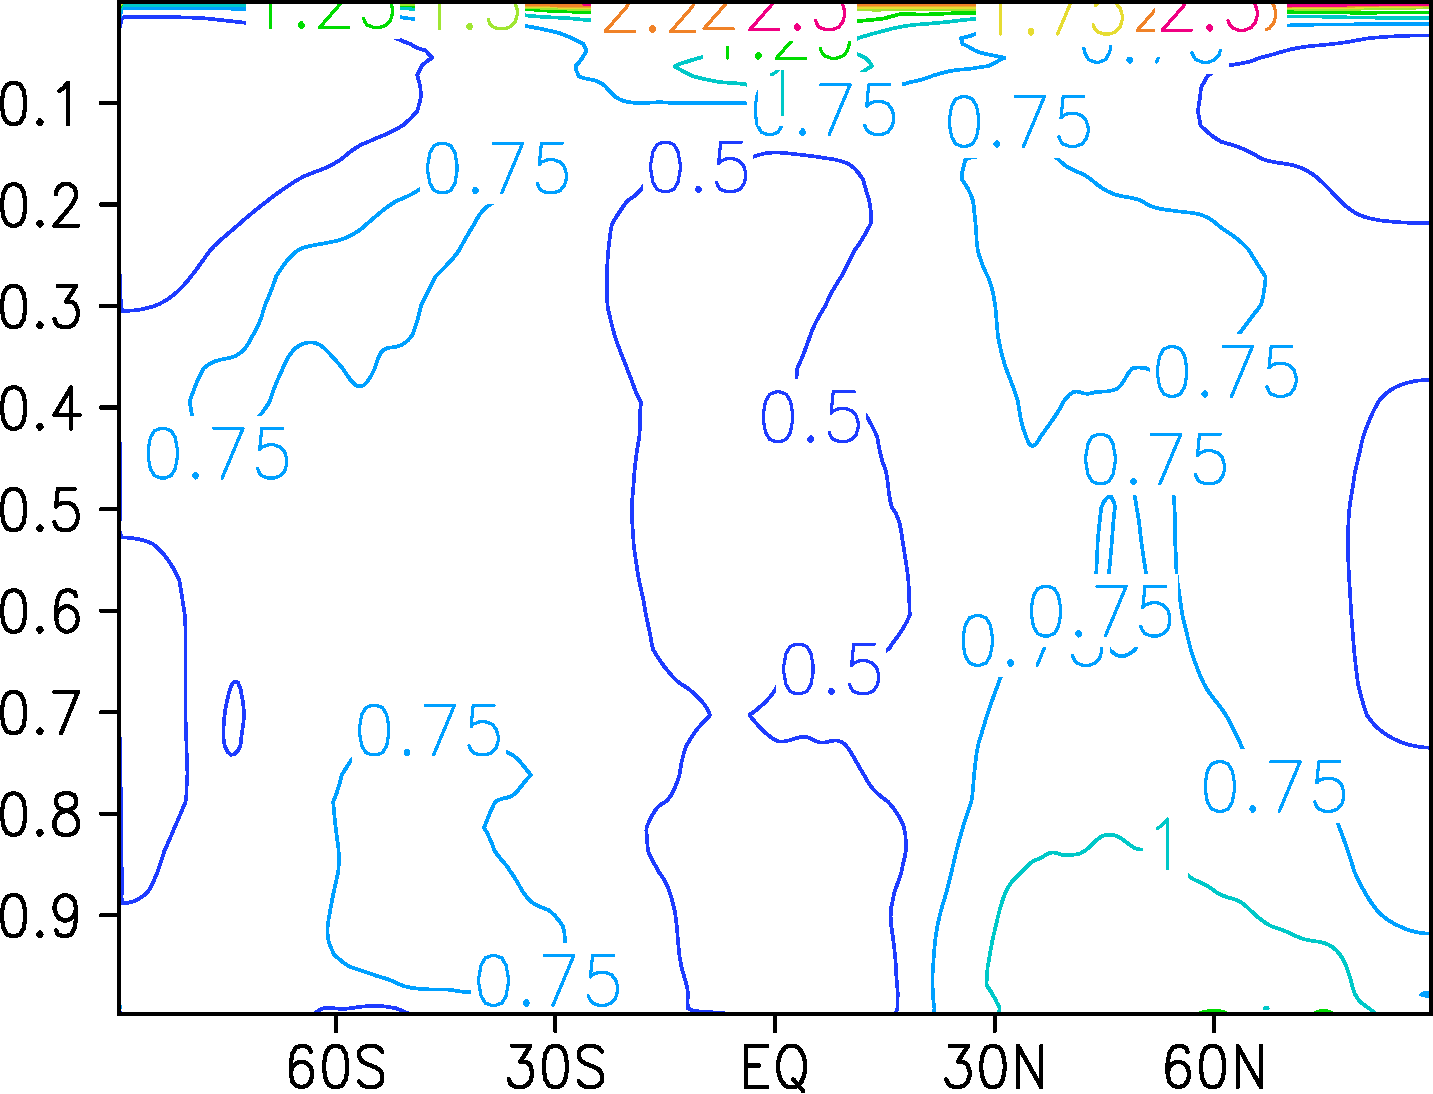
\includegraphics[width=0.3\textwidth,angle=0]{./figs/cap3/amplitudes_novas/amplitudes-BAllZ_t-crop-rotated270.pdf}
        }   
        \subfigure[$\mathbf{B}$ CPTEC (12Z), $T$]{
          \label{fig:bcptec_12z_t}
          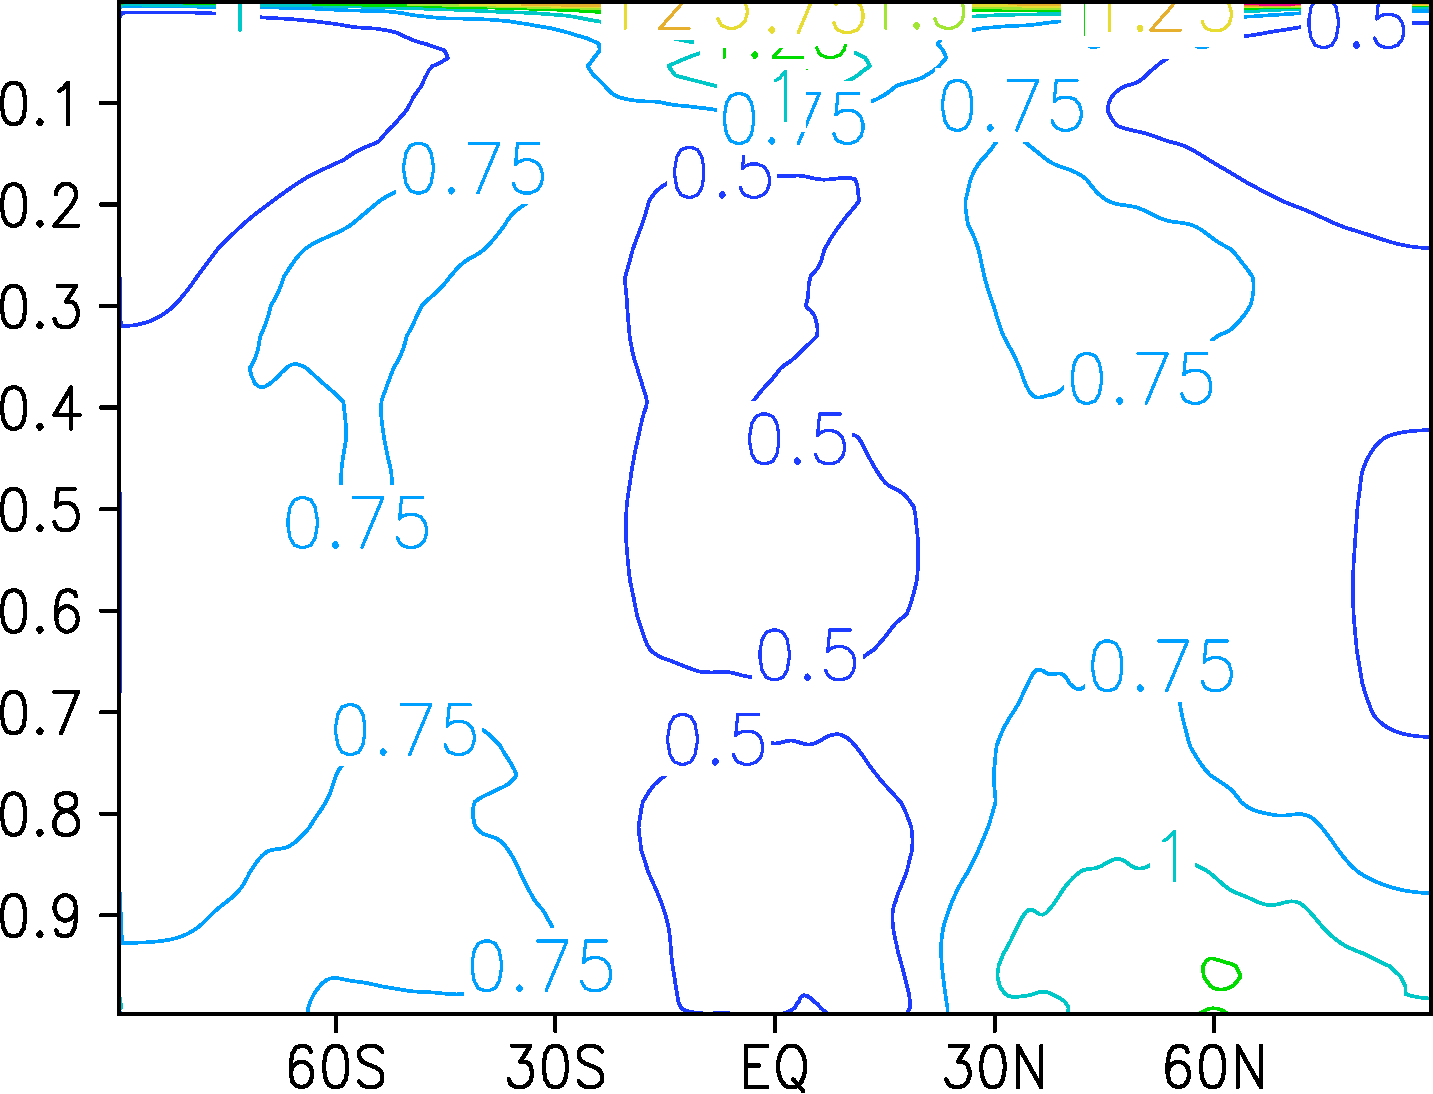
\includegraphics[width=0.3\textwidth,angle=0]{./figs/cap3/amplitudes_novas/amplitudes-B12Z_t-crop-rotated270.pdf}
        }    
        \subfigure[$\mathbf{B}$ CPTEC (18Z), $T$]{
          \label{fig:bcptec_18z_t}
          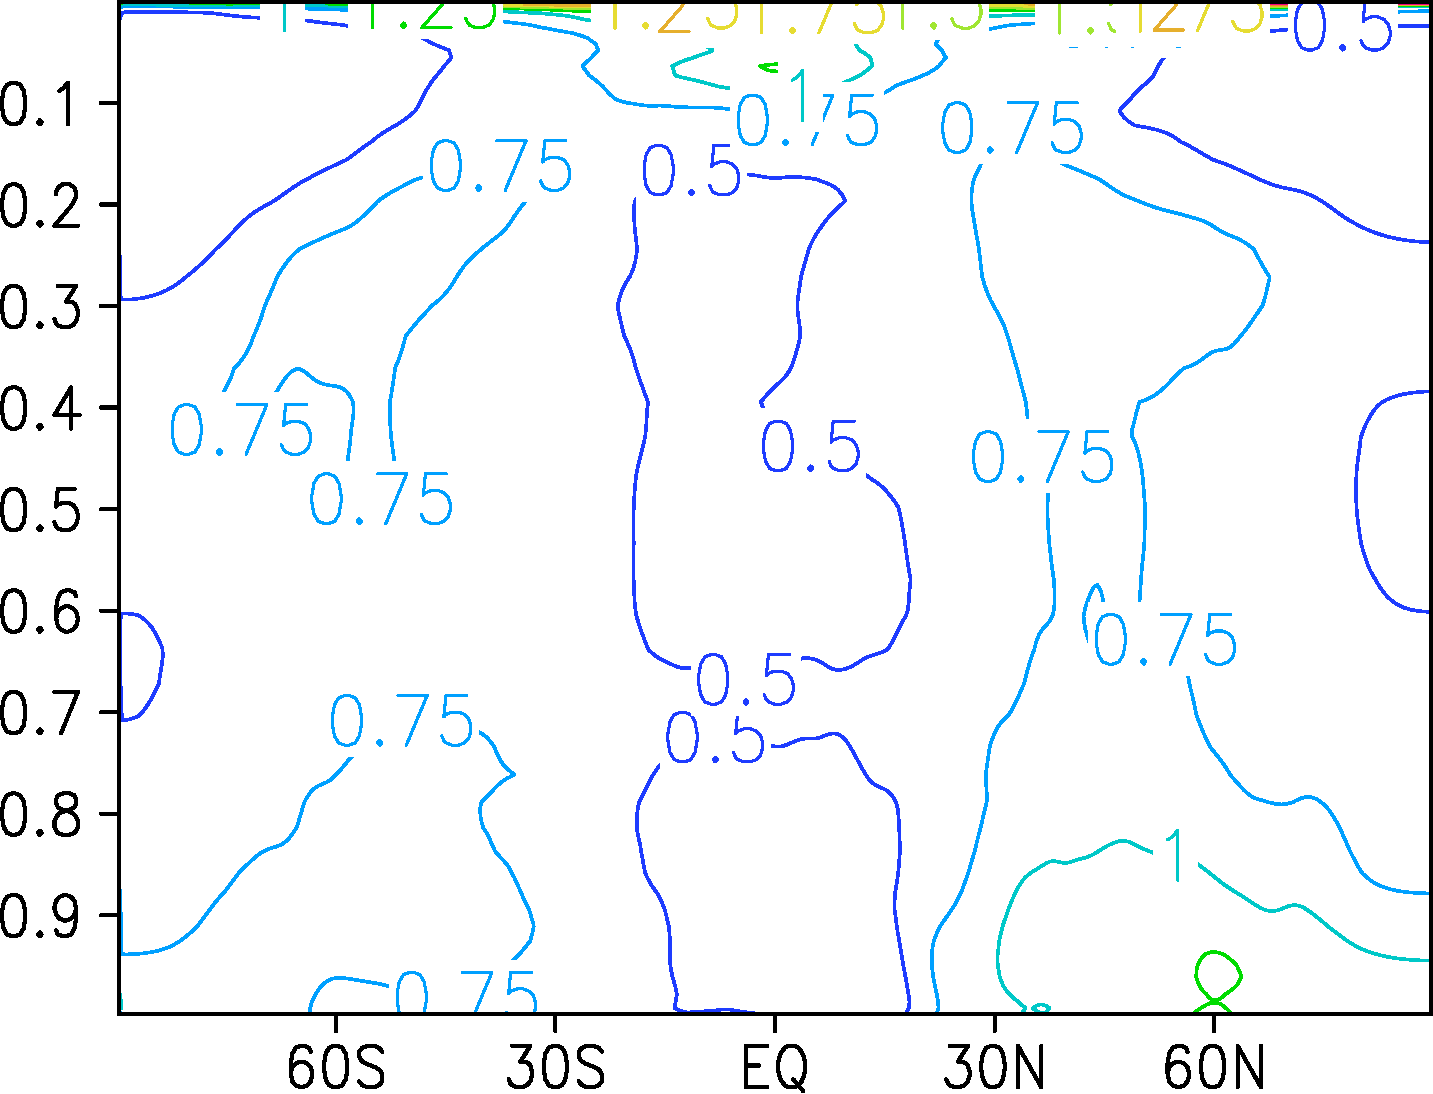
\includegraphics[width=0.3\textwidth,angle=0]{./figs/cap3/amplitudes_novas/amplitudes-B18Z_t-crop-rotated270.pdf}
        }   
  \end{center}
  \vspace{2mm}
  \legenda{}
  \label{fig:B_mcgav4_T}
  \FONTE{Produção do autor.}
\end{figure}

As amplitudes da umidade apresentada na Figura \ref{fig:bcptec_allz_q} para a matriz CPTEC BAllZ, não difere muito em distribuição ao longo das latitudes como nas demais matrizes (i.e., 00, 06, 12 e 18Z - Figuras \ref{fig:bcptec_00z_q}, \ref{fig:bcptec_06z_q}, \ref{fig:bcptec_12z_q} e \ref{fig:bcptec_18z_q}, respectivamente), mas a amplitude da variância nos subtrópicos em ambos os hemisférios (entre 60S e 30S e entre 30N e 60N), é melhor definida e menos intensa também do que aquela representada em B NCEP (Figura \ref{fig:bncep_allz_q}). Neste caso, a variância da umidade em ambos os hemisférios é bastante simétrica, principalmente nos casos calculados com as previsões do CPTEC. Isto pode reforçar a necessidade de se remover o viés do modelo do CPTEC. Neste caso, as isolinhas mais próximas a superfície (até o nível sigma 0.8 ou 819.2 hPa), apresentam valores com quase o dobro do valor, se comparados com a mesma região na matriz do NCEP. De outra forma, pode mostrar também alguma deficiência na física do modelo em representar com melhor precisão os processos úmidos (que dependem da física do modelo).

\begin{figure}[H]
    \vspace{2mm}
    \caption{Idem Figura \ref{fig:B_mcgav4_psi}, para a umidade ($q$).}
    \begin{center}
        \subfigure[$\mathbf{B}$ NCEP (ALLZ), $q$]{
          \label{fig:bncep_allz_q}
          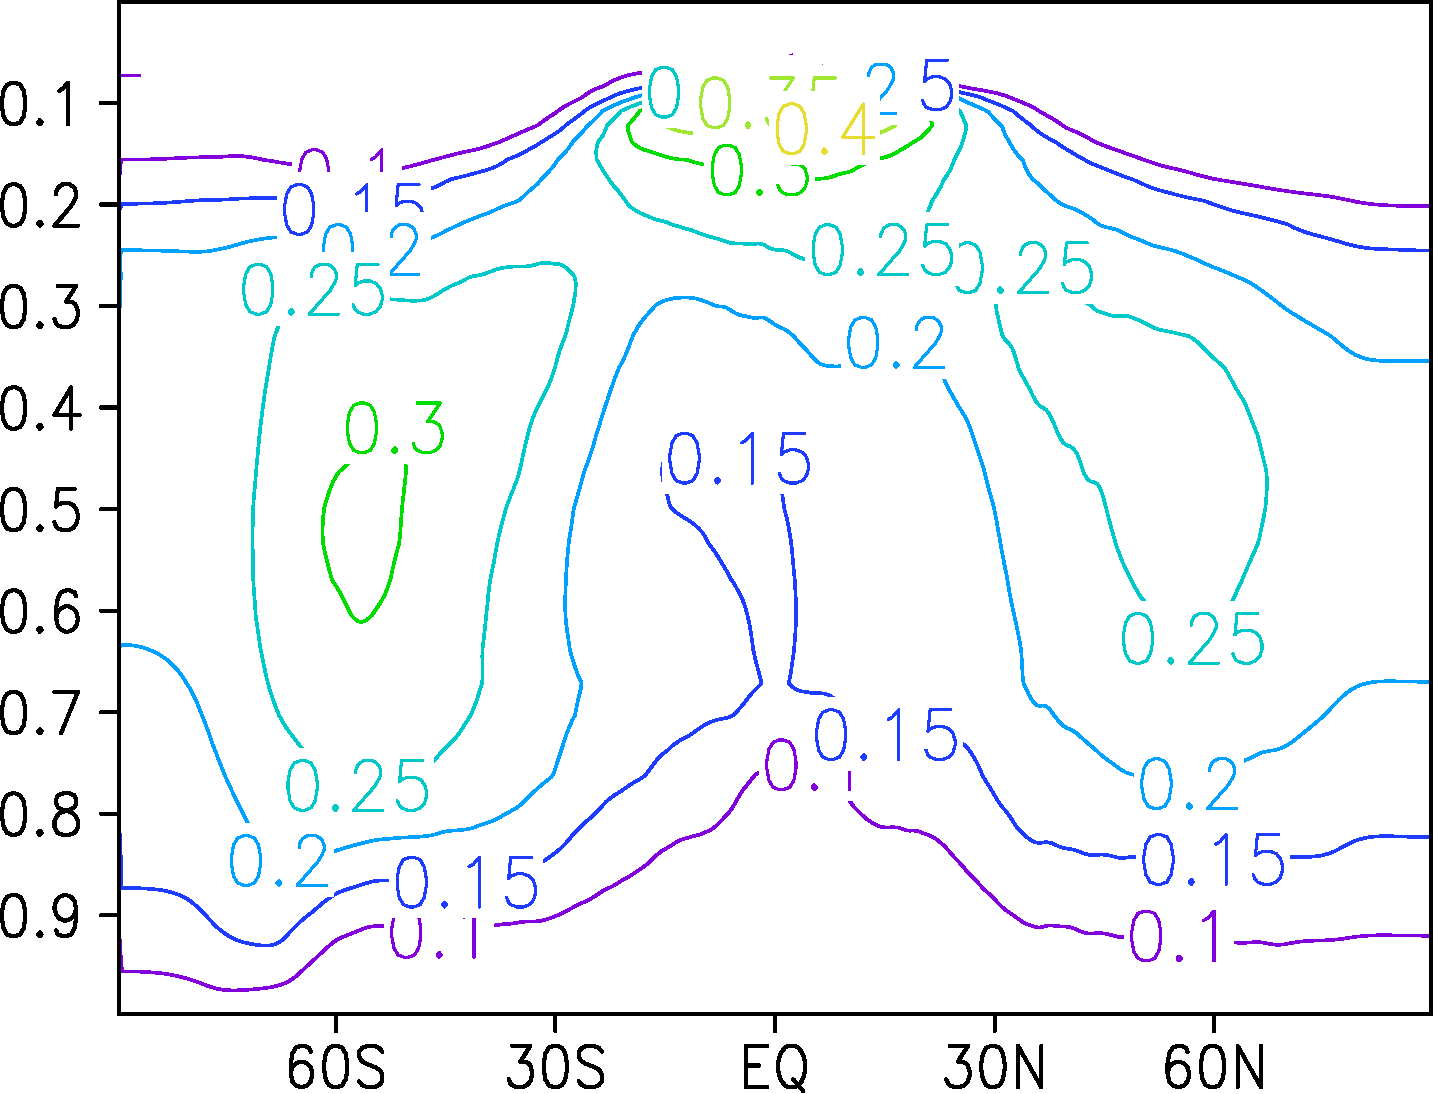
\includegraphics[width=0.3\textwidth,angle=0]{./figs/cap3/amplitudes_novas/amplitudes-NCEP_q-crop-rotated270.pdf} 
        }
        \subfigure[$\mathbf{B}$ CPTEC (00Z), $q$]{
          \label{fig:bcptec_00z_q}
          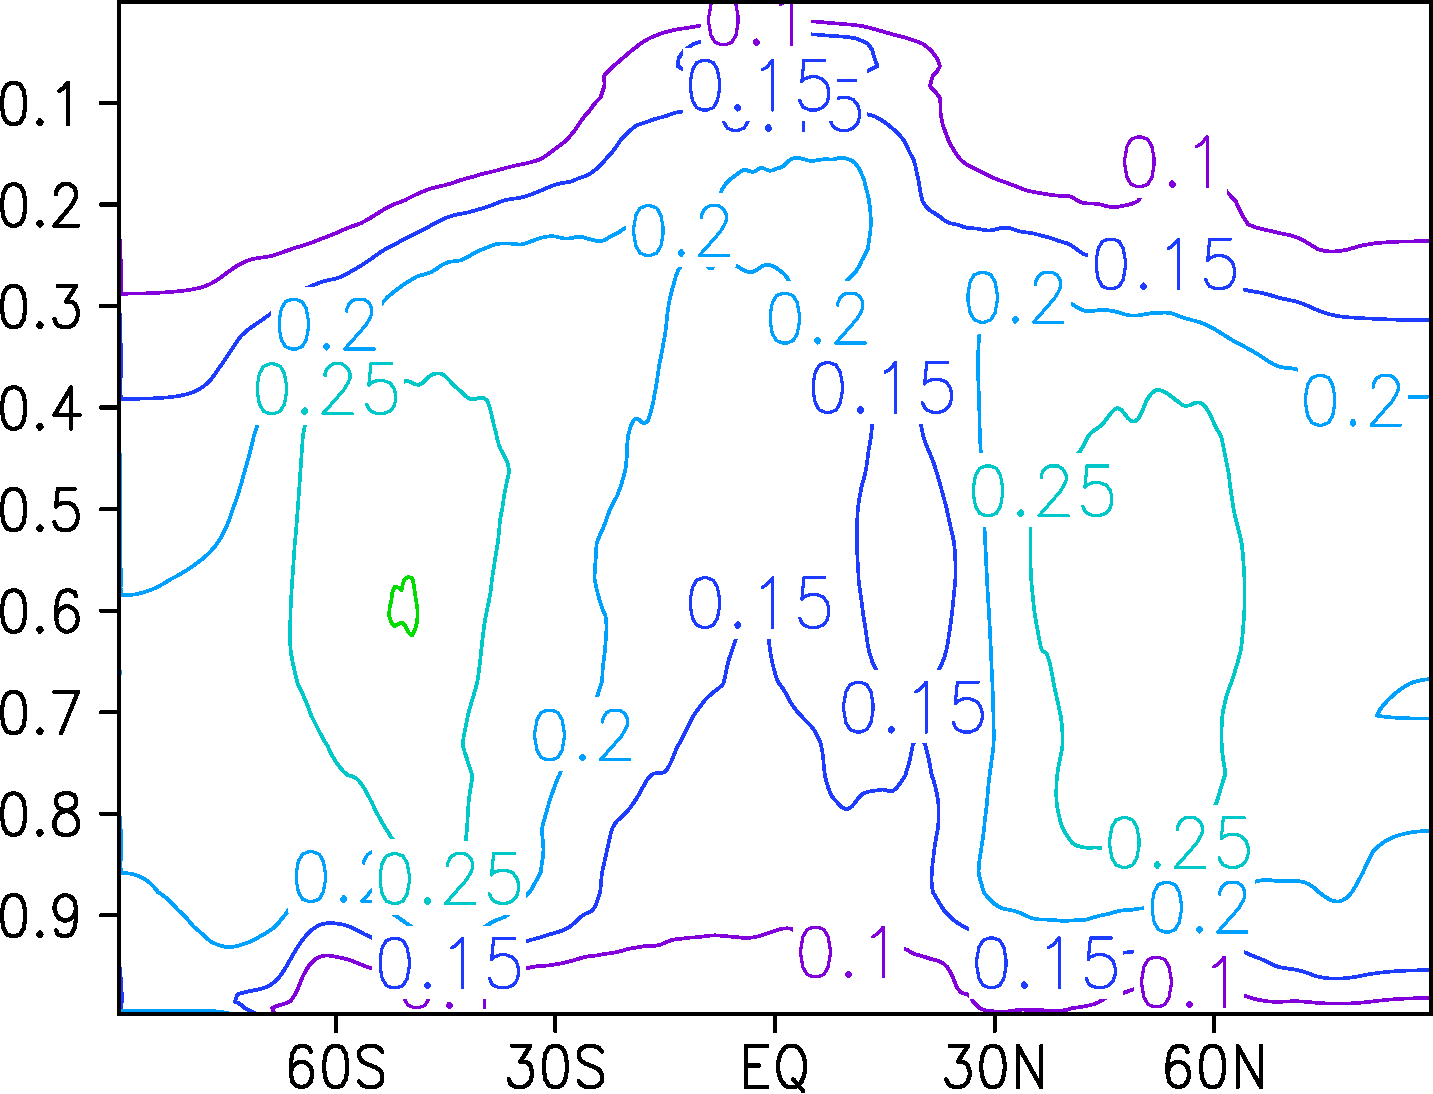
\includegraphics[width=0.3\textwidth,angle=0]{./figs/cap3/amplitudes_novas/amplitudes-B00Z_q-crop-rotated270.pdf}
        } 
        \subfigure[$\mathbf{B}$ CPTEC (06Z), $q$]{
          \label{fig:bcptec_06z_q}
          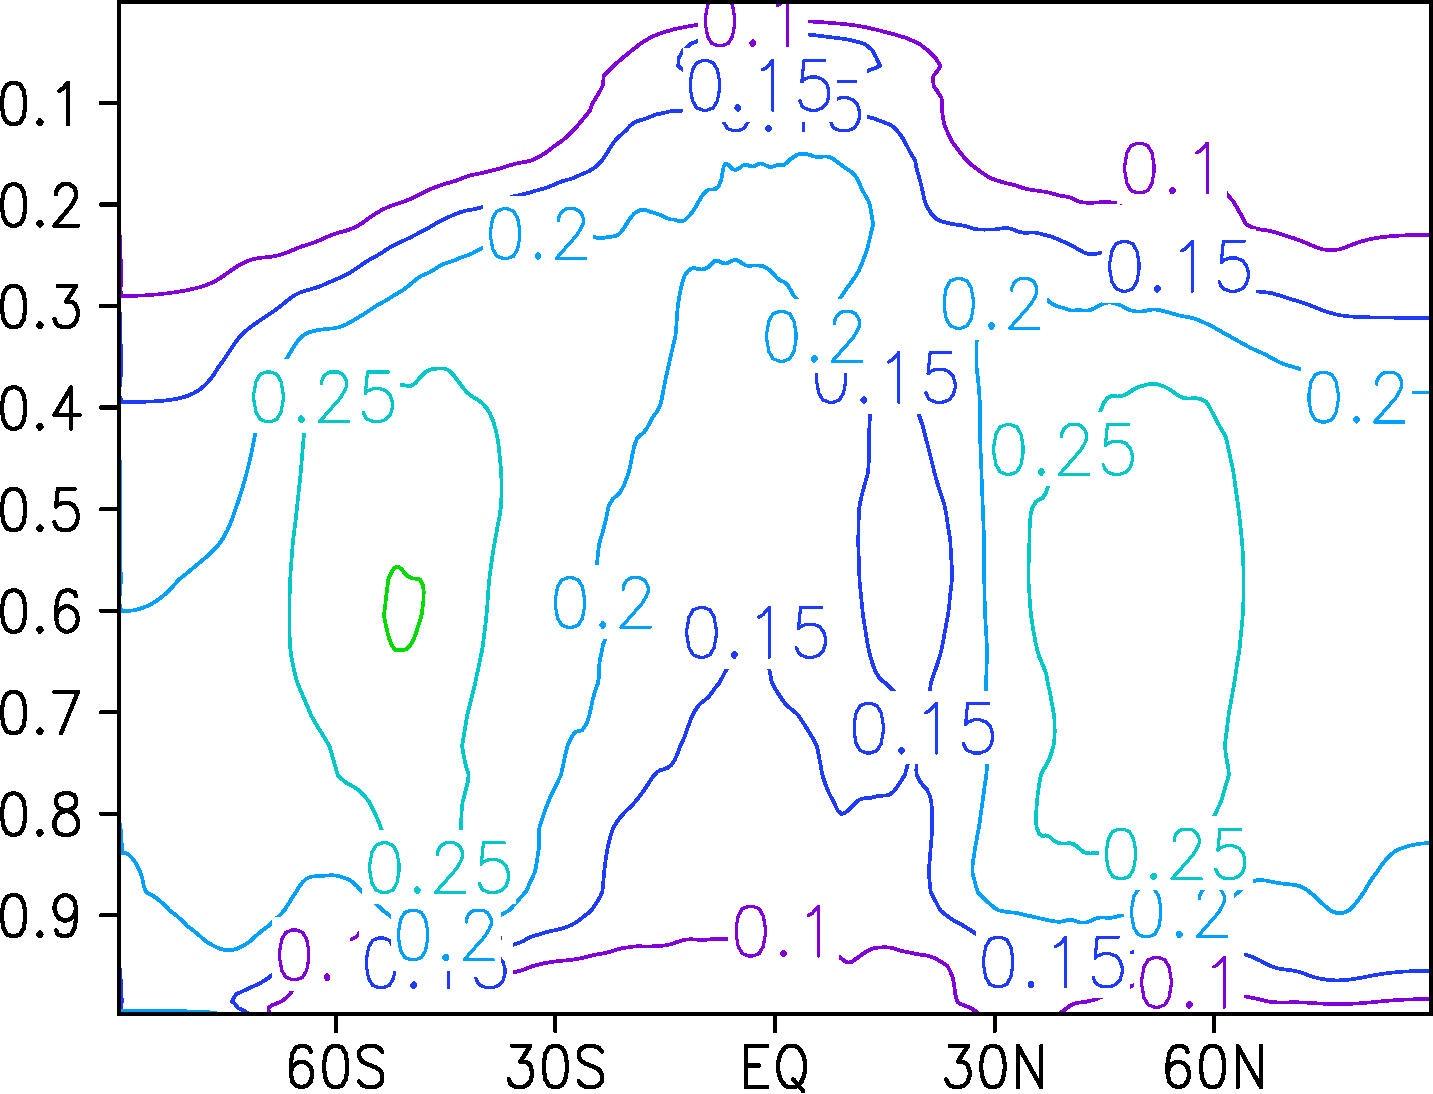
\includegraphics[width=0.3\textwidth,angle=0]{./figs/cap3/amplitudes_novas/amplitudes-B06Z_q-crop-rotated270.pdf}
        } \\
        
        \subfigure[$\mathbf{B}$ CPTEC (ALLZ), $q$]{
          \label{fig:bcptec_allz_q}
          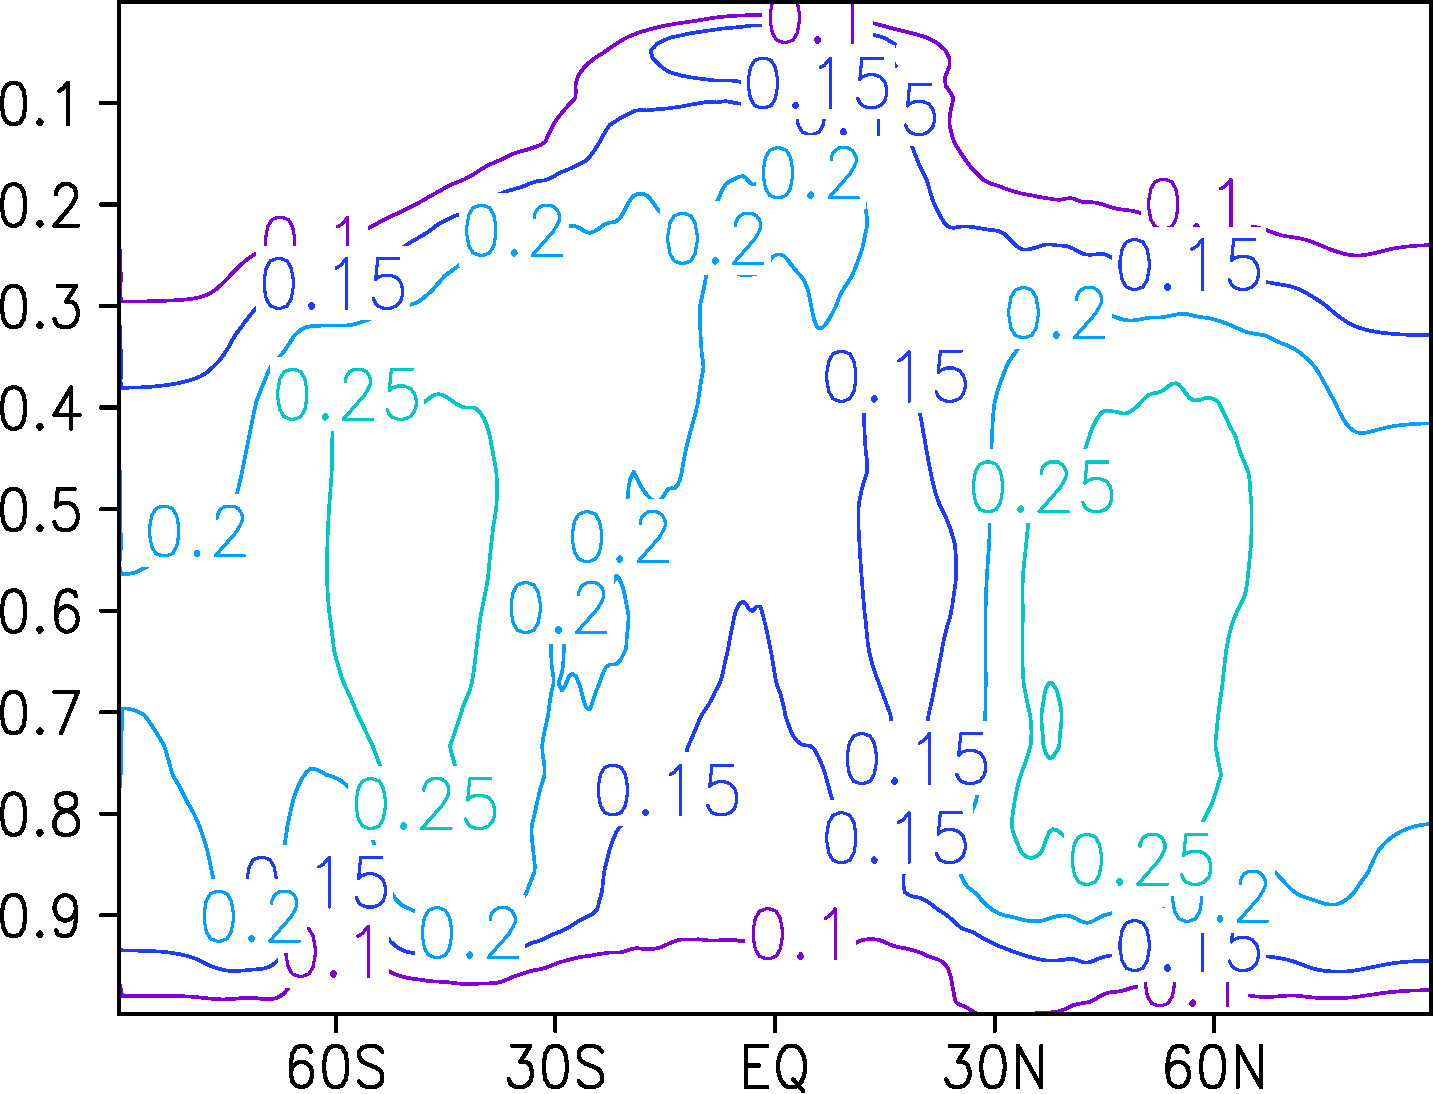
\includegraphics[width=0.3\textwidth,angle=0]{./figs/cap3/amplitudes_novas/amplitudes-BAllZ_q-crop-rotated270.pdf}
        }   
        \subfigure[$\mathbf{B}$ CPTEC (12Z), $q$]{
          \label{fig:bcptec_12z_q}
          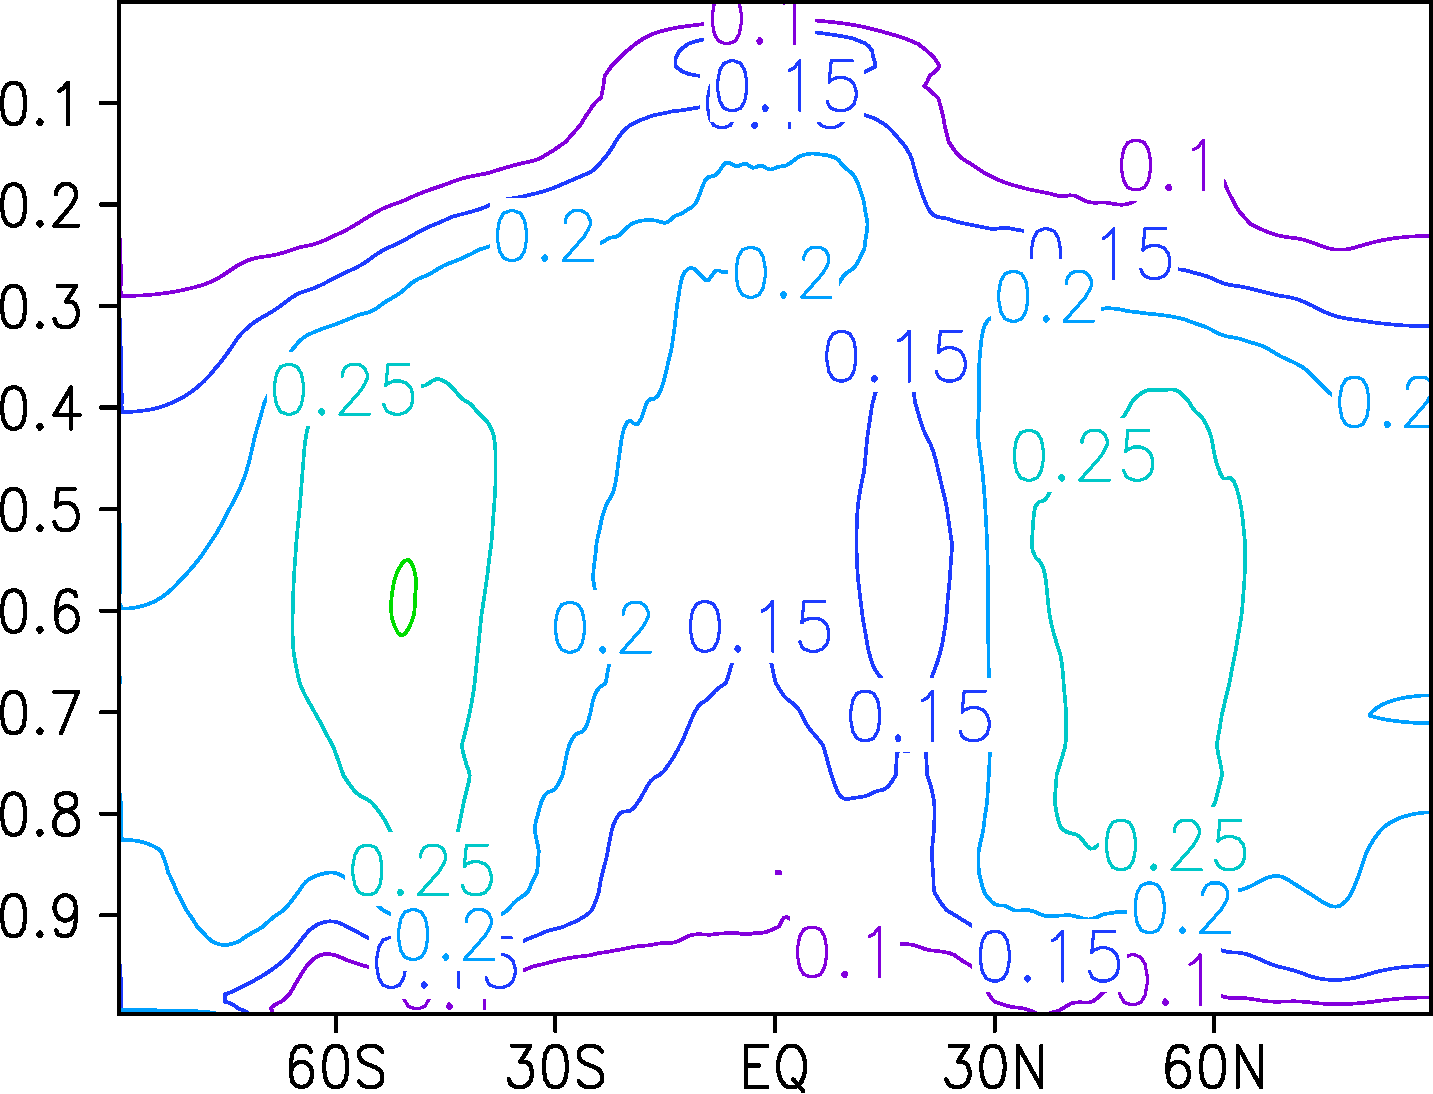
\includegraphics[width=0.3\textwidth,angle=0]{./figs/cap3/amplitudes_novas/amplitudes-B12Z_q-crop-rotated270.pdf}
        }    
        \subfigure[$\mathbf{B}$ CPTEC (18Z), $q$]{
          \label{fig:bcptec_18z_q}
          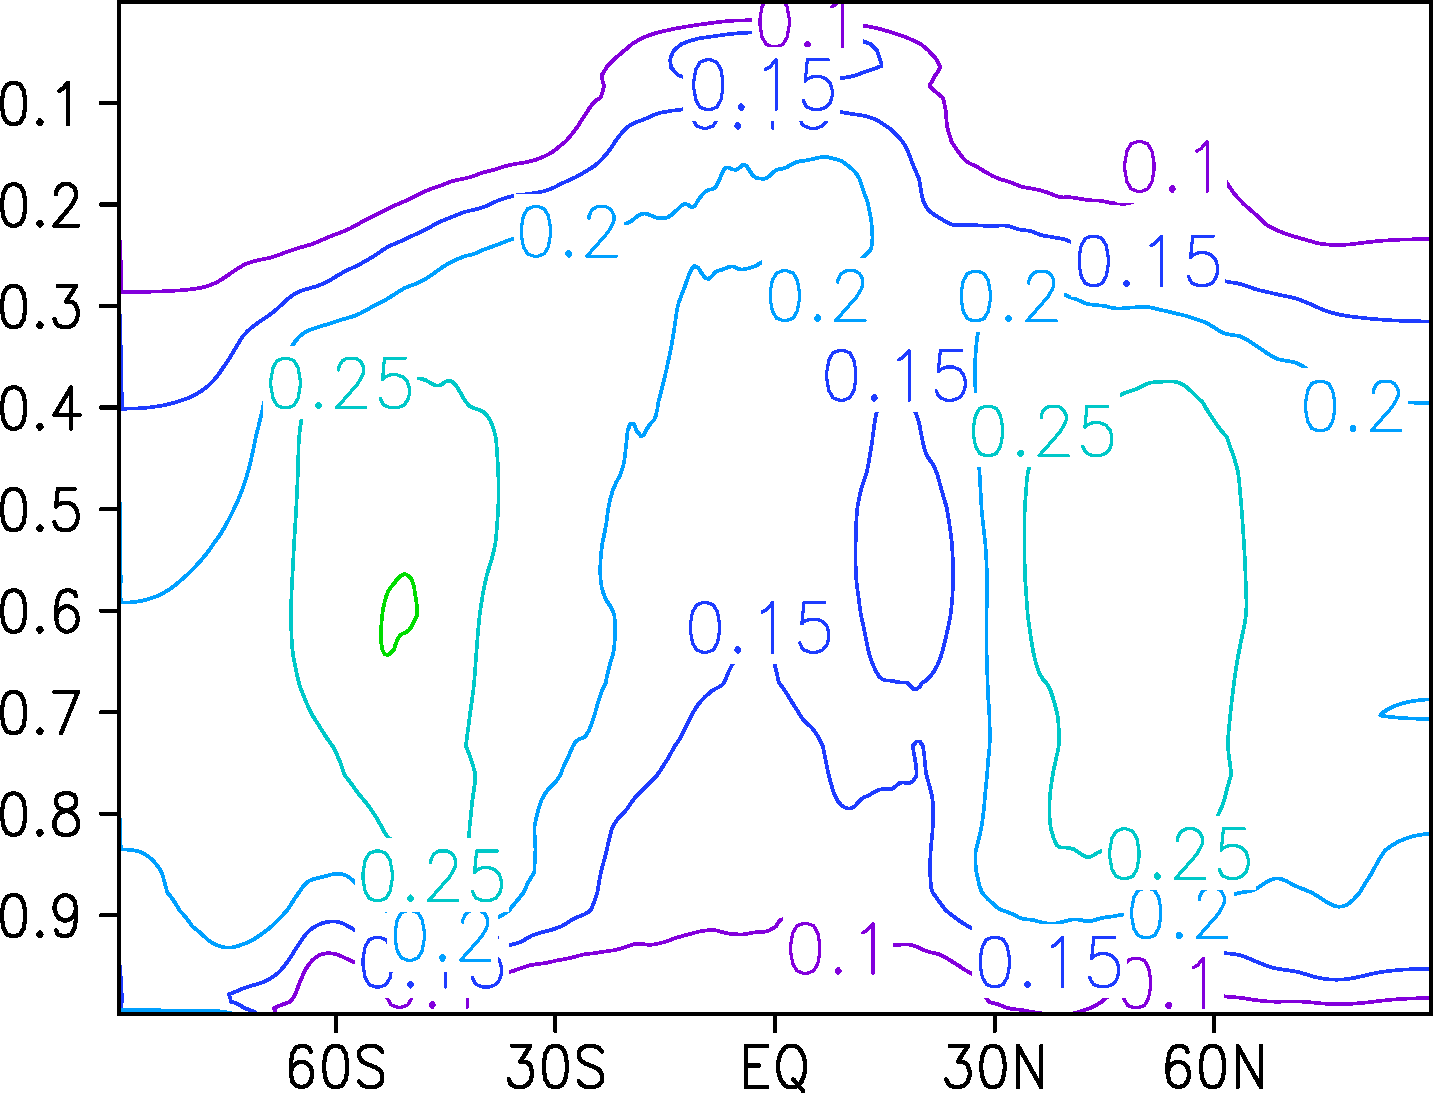
\includegraphics[width=0.3\textwidth,angle=0]{./figs/cap3/amplitudes_novas/amplitudes-B18Z_q-crop-rotated270.pdf}
        }   
  \end{center}
  \vspace{2mm}
  \legenda{}
  \label{fig:B_mcgav4_q}
  \FONTE{Produção do autor.}
\end{figure}

A Figura \ref{fig:B_mcgav4_ps} apresenta a distribuição latitudinal das médias zonais das amplitudes da pressão em superfície. As amplitudes da matriz B NCEP (Figura \ref{fig:bncep_allz_ps}) apresentam uma distribuição simétrica, com dois picos sobre as latitudes de 60S e 60N. Nas matrizes do CPTEC (Figuras \ref{fig:bcptec_00z_ps}, \ref{fig:bcptec_06z_ps}, \ref{fig:bcptec_allz_ps}, \ref{fig:bcptec_12z_ps} e \ref{fig:bcptec_18z_ps}), a distribuição das amplitudes é assimétrica, sendo que os picos das amplitudes são maiores sobre a latitude de 60N do que sobre a latitude de 60S. A mesma amplitude apresentada em \citeonline{wuetal/2002}, mostra que os picos da variância dos erros situam-se em torno destas latitudes, especialmente sobre o Hemisfério Norte, onde o pico local situa-se entre as latitudes de 30N e 60N.

\begin{figure}[H]
  \vspace{2mm}
    \caption{Idem Figura \ref{fig:B_mcgav4_psi}, para a pressão em superfície ($ps$, x $10^{2}$).}
    \begin{center}
        \subfigure[$\mathbf{B}$ NCEP (ALLZ), $ps$]{
          \label{fig:bncep_allz_ps}
          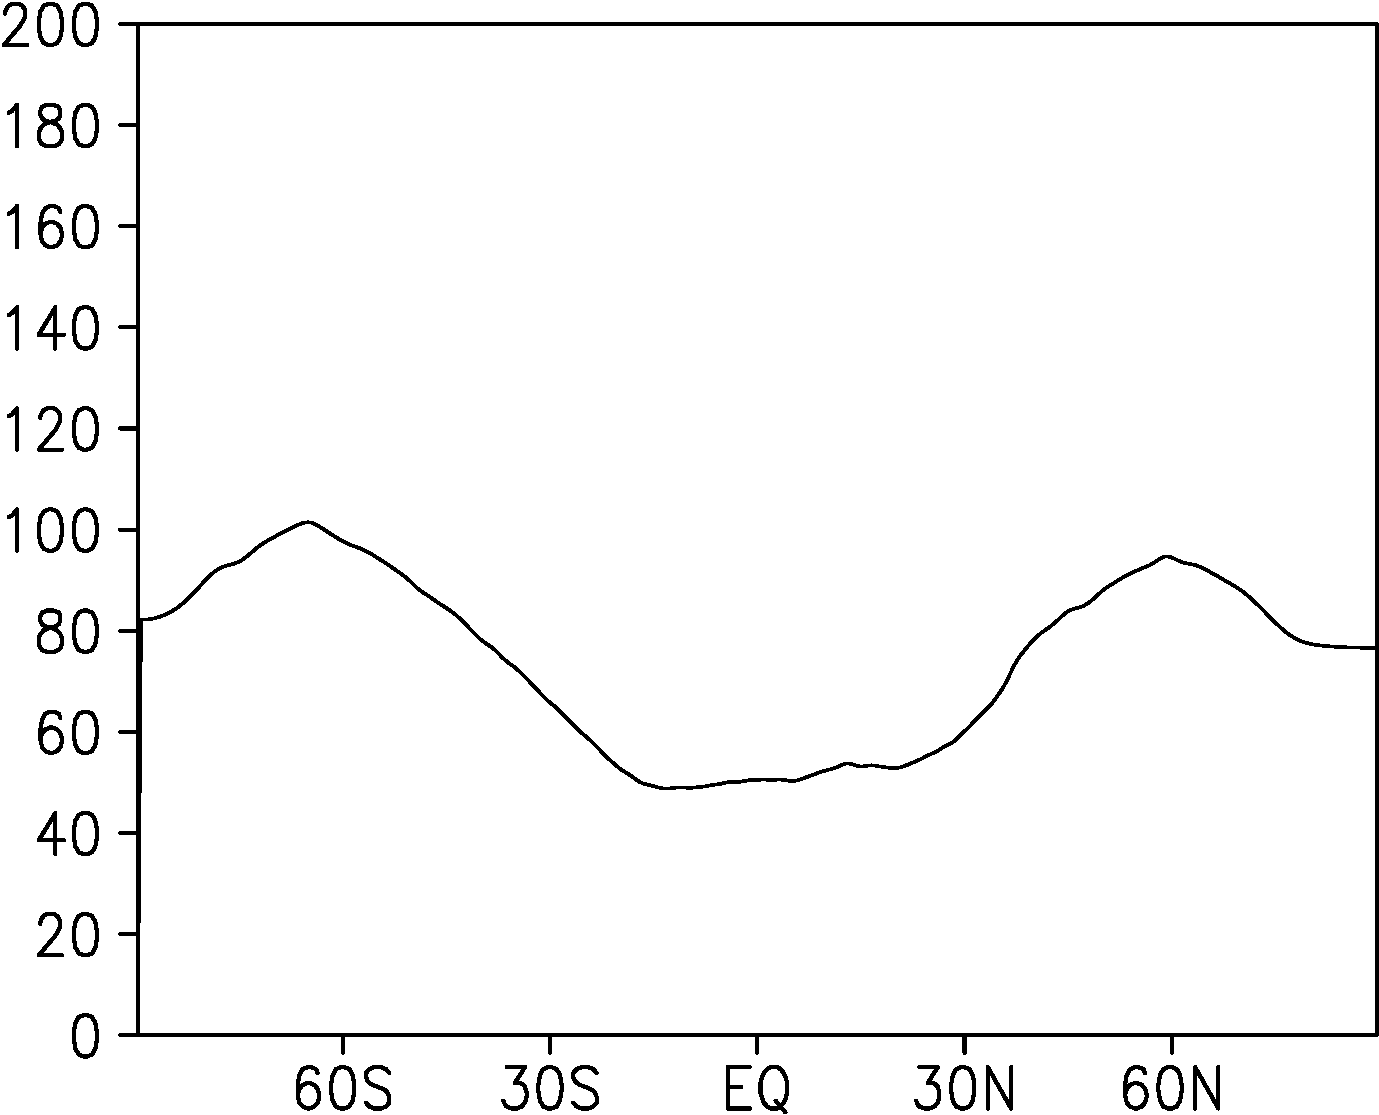
\includegraphics[width=0.3\textwidth,angle=0]{./figs/cap3/amplitudes_novas/amplitudes-NCEP_ps-crop-rotated270.pdf}
        }
        \subfigure[$\mathbf{B}$ CPTEC (00Z), $ps$]{
          \label{fig:bcptec_00z_ps}
          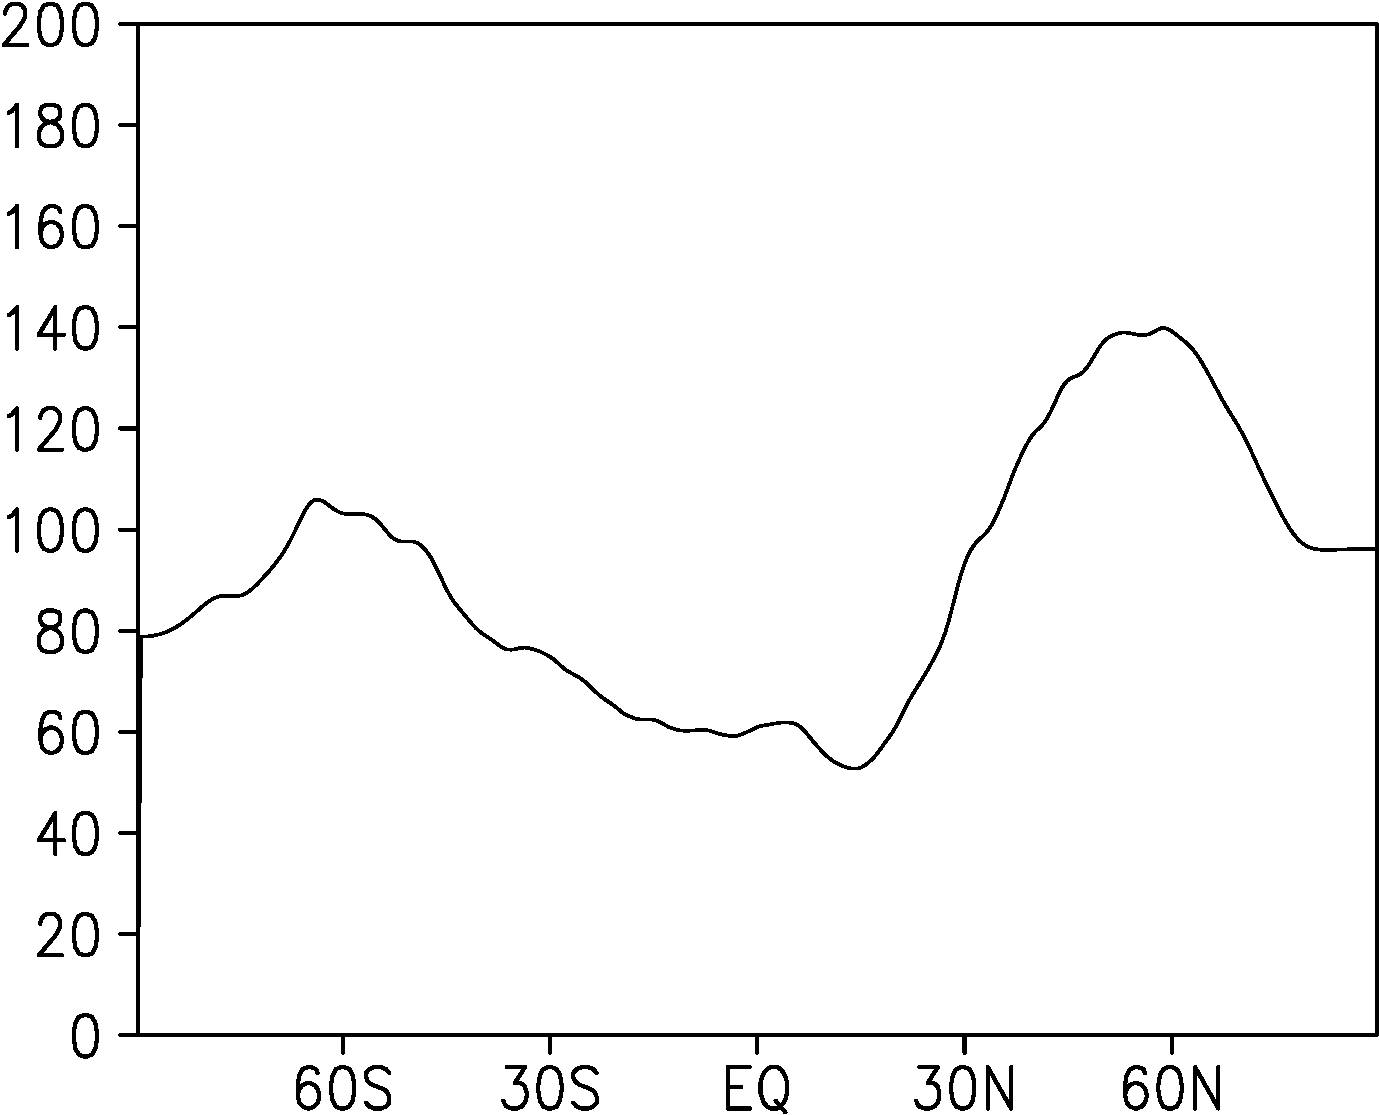
\includegraphics[width=0.3\textwidth,angle=0]{./figs/cap3/amplitudes_novas/amplitudes-B00Z_ps-crop-rotated270.pdf}
        } 
        \subfigure[$\mathbf{B}$ CPTEC (06Z), $ps$]{
          \label{fig:bcptec_06z_ps}
          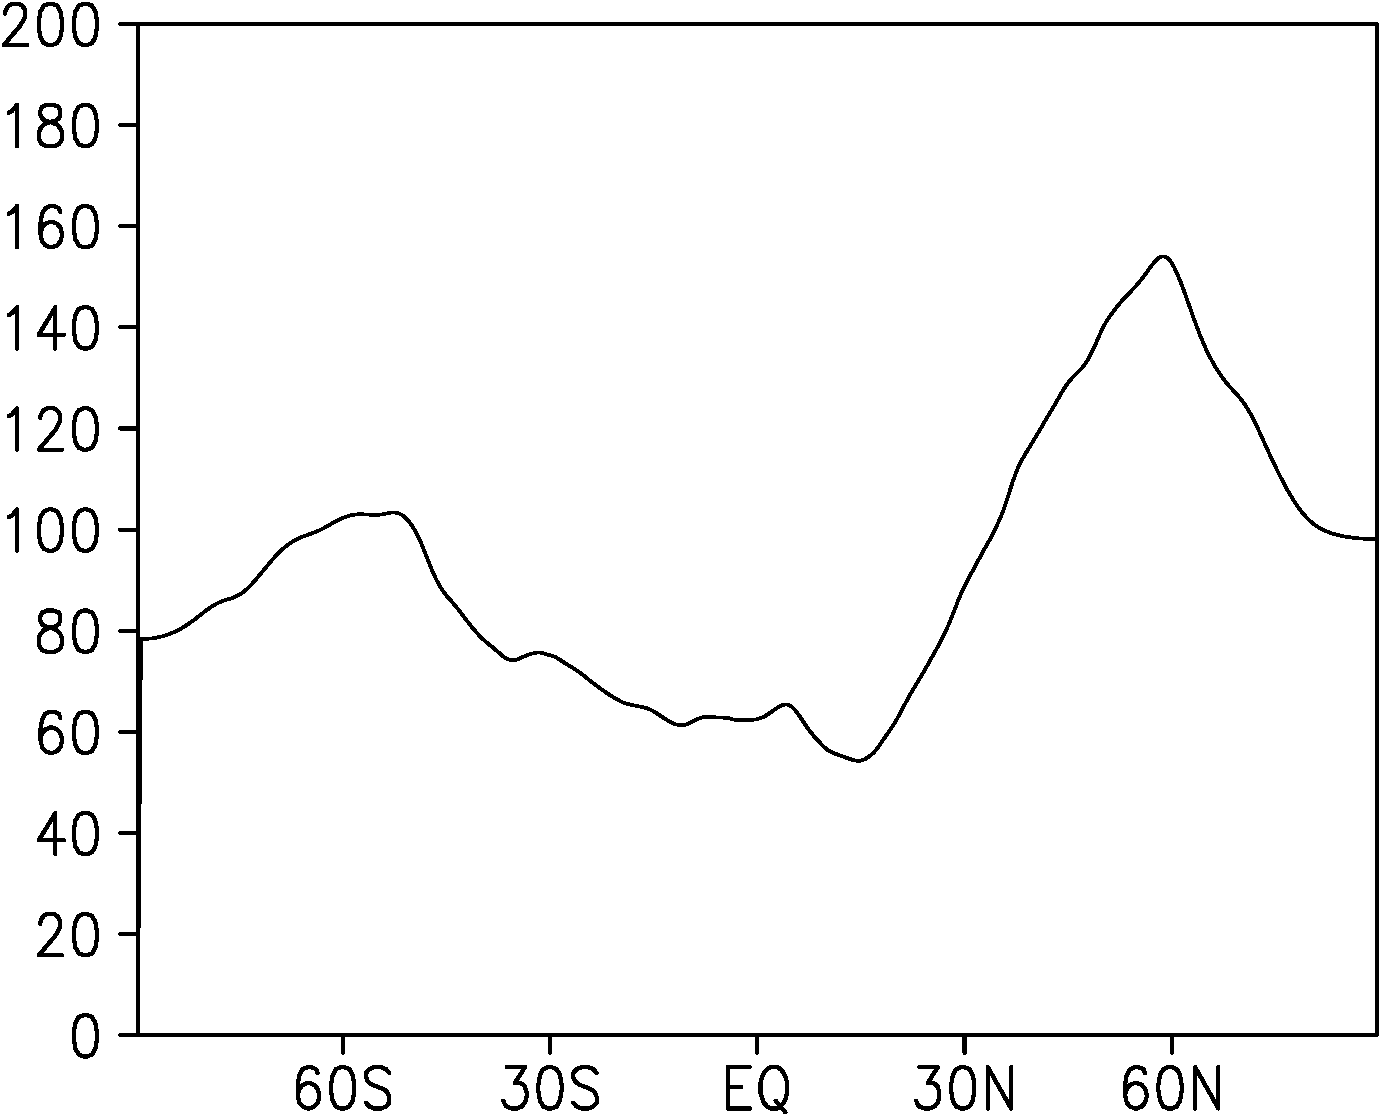
\includegraphics[width=0.3\textwidth,angle=0]{./figs/cap3/amplitudes_novas/amplitudes-B06Z_ps-crop-rotated270.pdf}
        } \\
        
        \subfigure[$\mathbf{B}$ CPTEC (ALLZ), $ps$]{
          \label{fig:bcptec_allz_ps}
          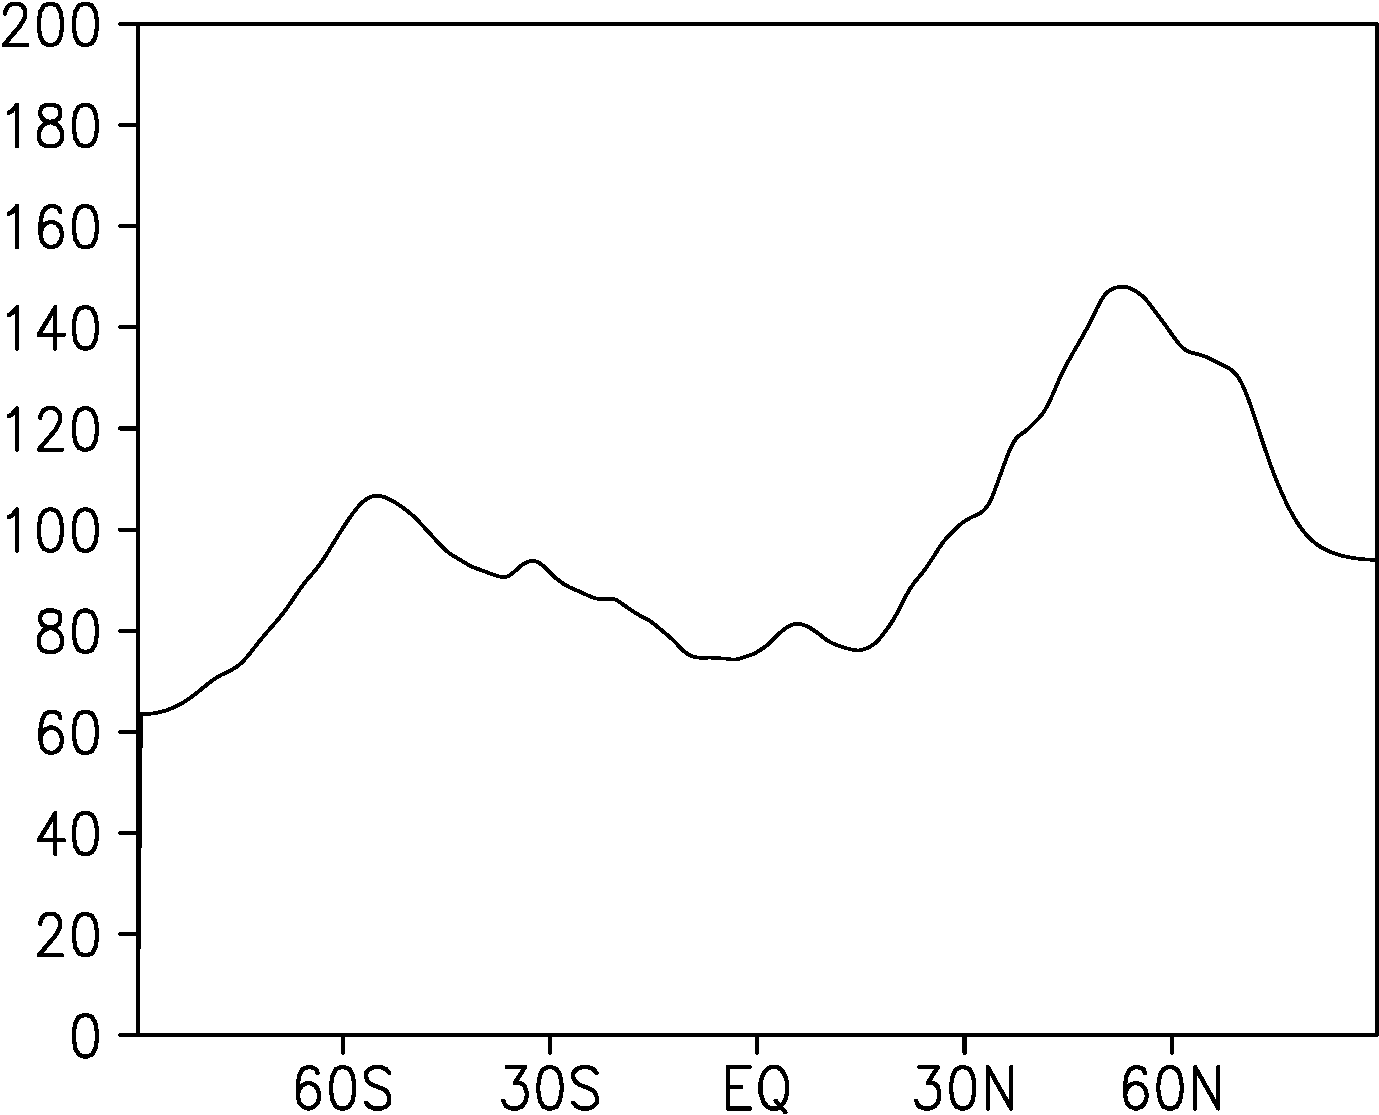
\includegraphics[width=0.3\textwidth,angle=0]{./figs/cap3/amplitudes_novas/amplitudes-BAllZ_ps-crop-rotated270.pdf}
        }   
        \subfigure[$\mathbf{B}$ CPTEC (12Z), $ps$]{
          \label{fig:bcptec_12z_ps}
          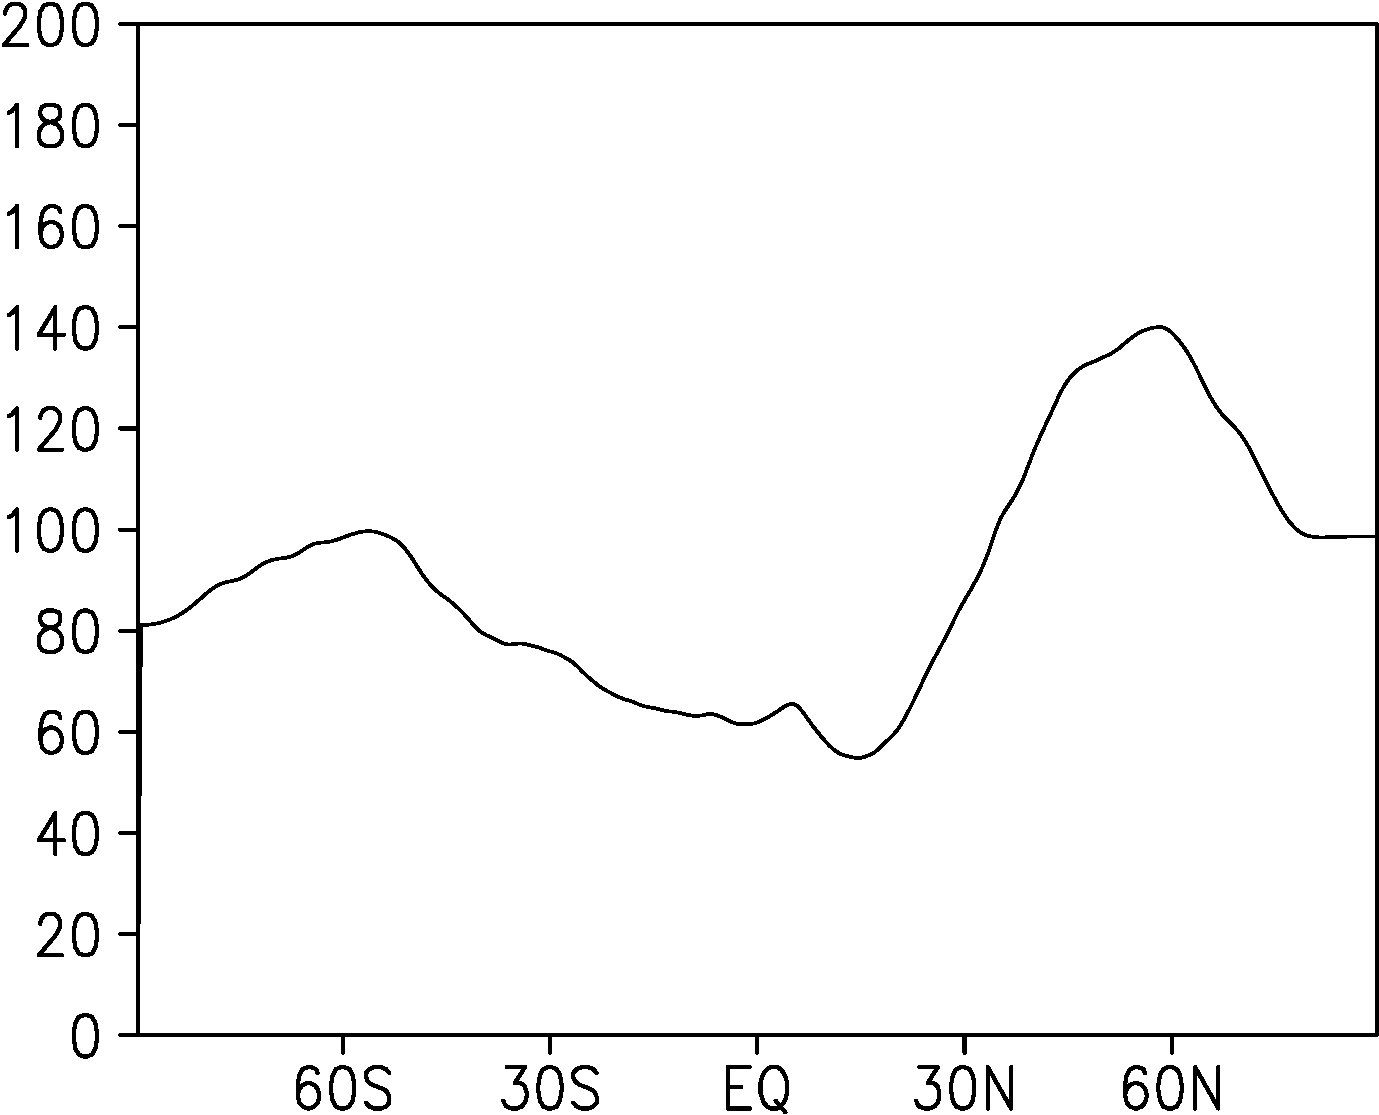
\includegraphics[width=0.3\textwidth,angle=0]{./figs/cap3/amplitudes_novas/amplitudes-B12Z_ps-crop-rotated270.pdf}
        }    
        \subfigure[$\mathbf{B}$ CPTEC (18Z), $ps$]{
          \label{fig:bcptec_18z_ps}
          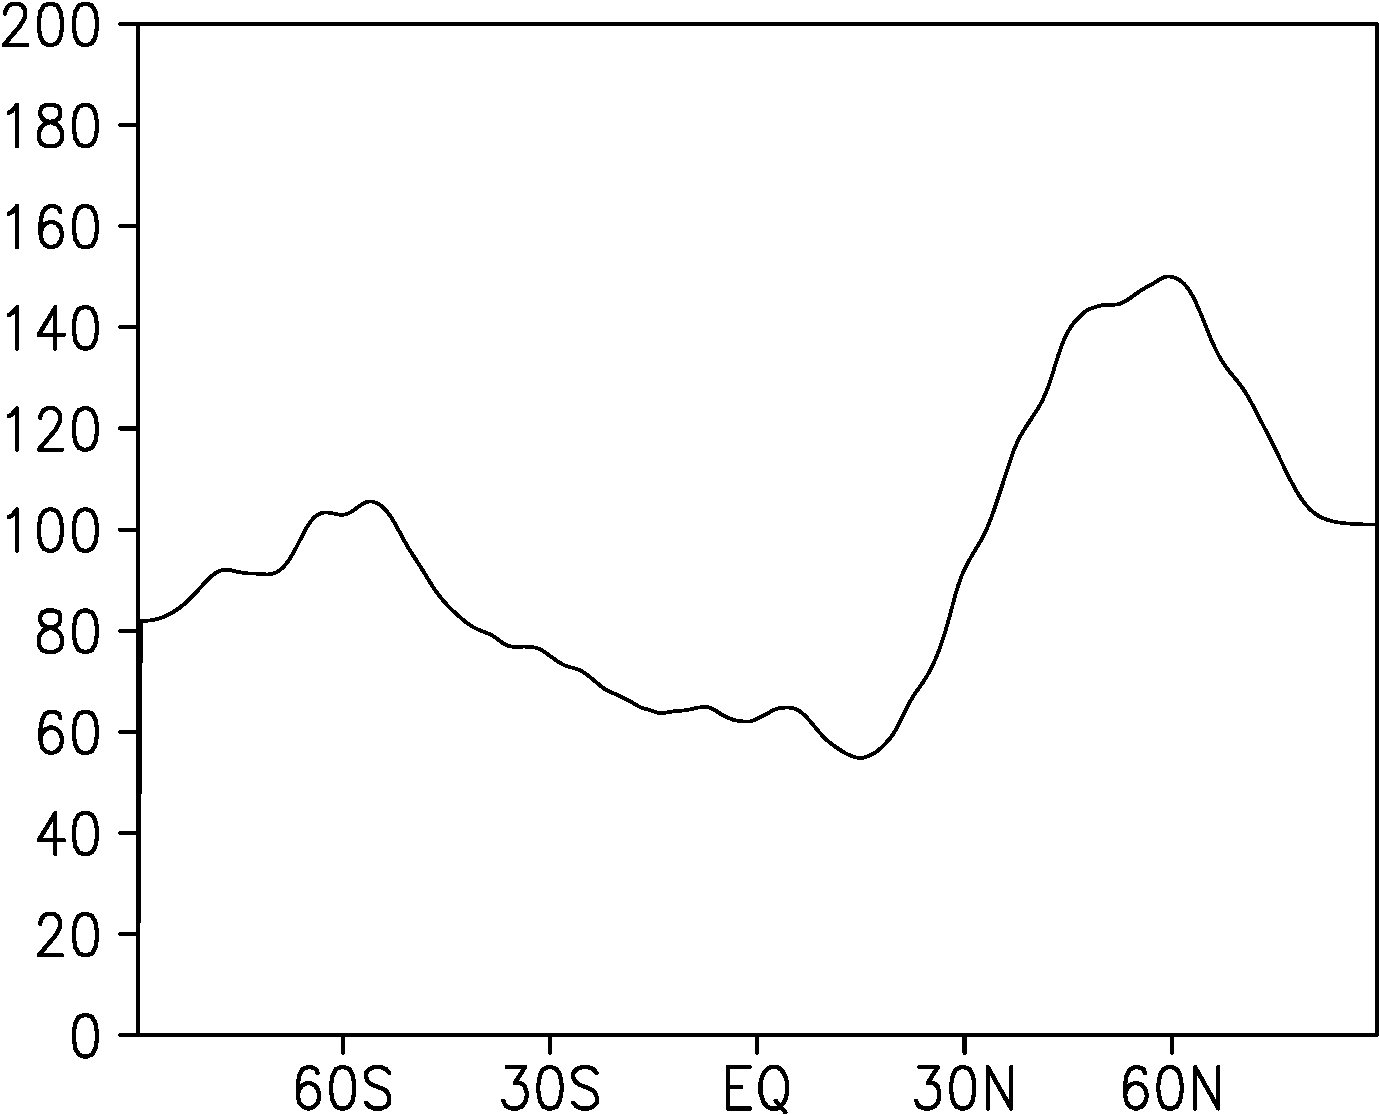
\includegraphics[width=0.3\textwidth,angle=0]{./figs/cap3/amplitudes_novas/amplitudes-B18Z_ps-crop-rotated270.pdf}
        }   
  \end{center} 
  \vspace{2mm}
  \legenda{}
  \label{fig:B_mcgav4_ps}
  \FONTE{Produção do autor.}
\end{figure}

As Figuras \ref{fig:bncep_allz_oz_zlog}, \ref{fig:bcptec_00z_oz} e a Figura \ref{fig:bcptec_allz_cw} mostram as amplitudes calculadas para as variáveis ozônio e razão de mistura de condensação em nuvem, respectivamente. O sistema G3DVAR (versão v1.1.3) não assimila observações e ozônio, e além disso, o ozônio utilizado pelo modelo de MCGAv4 utiliza uma climatologia do ozônio. As amplitudes calculadas para esta quantidade são bastante diferentes daquelas apresentadas pela matriz NCEP BAllZ (Figuras \ref{fig:bncep_allz_oz_zlog}, \ref{fig:bcptec_00z_oz}), e mostram valores muito mais altos do que qualquer matriz calculada utilizando-se os pares de previsões do CPTEC. Além disso, o MCGAv4 não representa a razão de mistura de condensação, como pode ser visto na Figura \ref{fig:bcptec_allz_cw}. Para melhorar a visualização da distribuição das amplitudes do ozônio, na Figura \ref{fig:bncep_allz_oz_zlog} estas amplitudes estão destacadas em escala logarítmica. 

\begin{figure}[H]
  \vspace{2mm}
    \caption{Idem Figura \ref{fig:B_mcgav4_psi}, para o ozônio ($oz$ x $10^{7}$) e o conteúdo de água ($cw$  x $10^{4}$).}
    \begin{center}
        \subfigure[$\mathbf{B}$ NCEP (ALLZ), $log(oz)$]{
          \label{fig:bncep_allz_oz_zlog}
          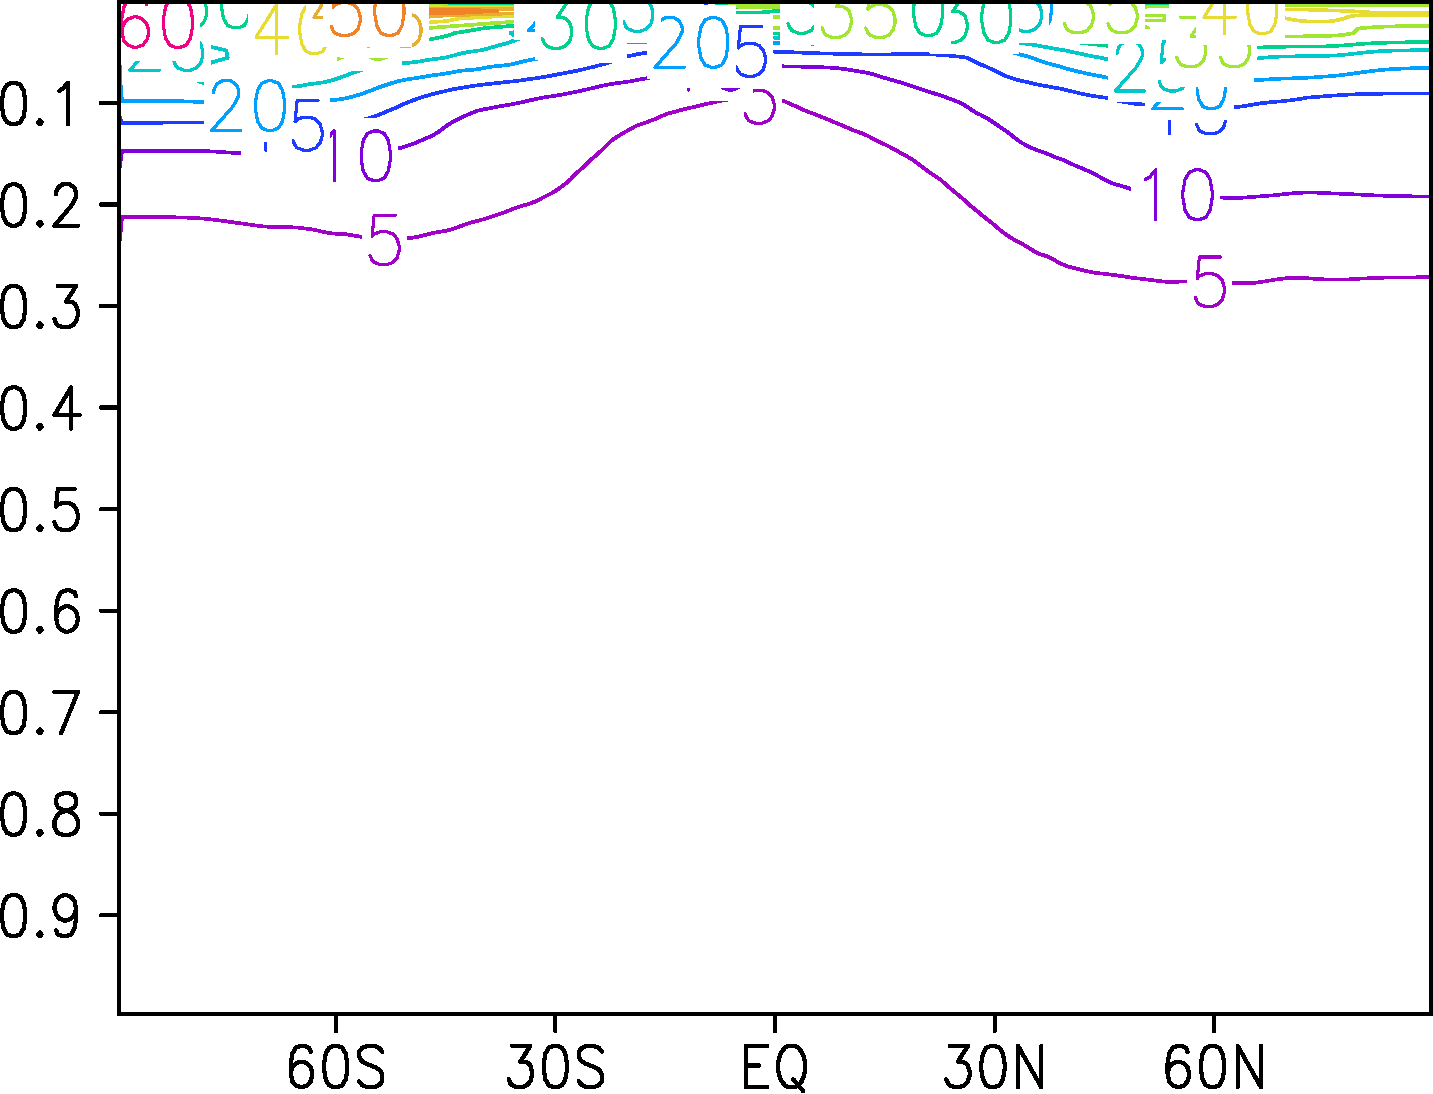
\includegraphics[width=0.3\textwidth,angle=0]{./figs/cap3/amplitudes_novas/amplitudes-NCEP_oz-orig-crop-rotated270.pdf}
        }
        \subfigure[$\mathbf{B}$ NCEP (ALLZ), $oz$]{
          \label{fig:bcptec_00z_oz}
          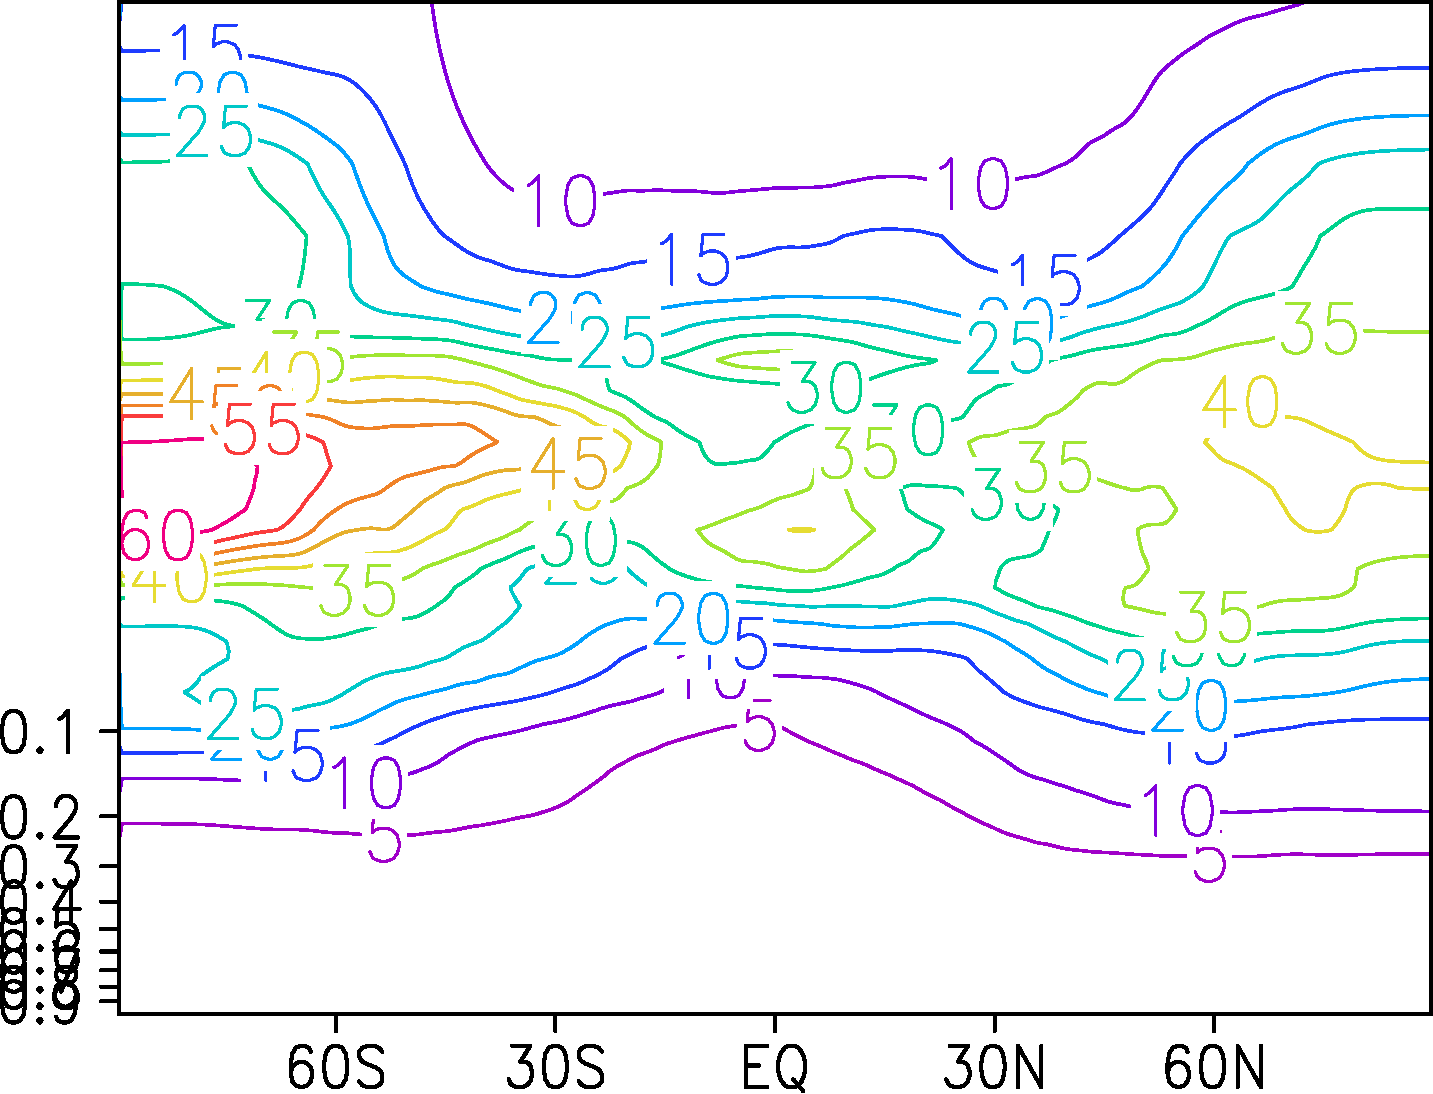
\includegraphics[width=0.3\textwidth,angle=0]{./figs/cap3/amplitudes_novas/amplitudes-NCEP_oz_zlog-orig-crop-rotated270.pdf}
        }         
        \subfigure[$\mathbf{B}$ NCEP (ALLZ), $cw$]{
          \label{fig:bcptec_allz_cw}
          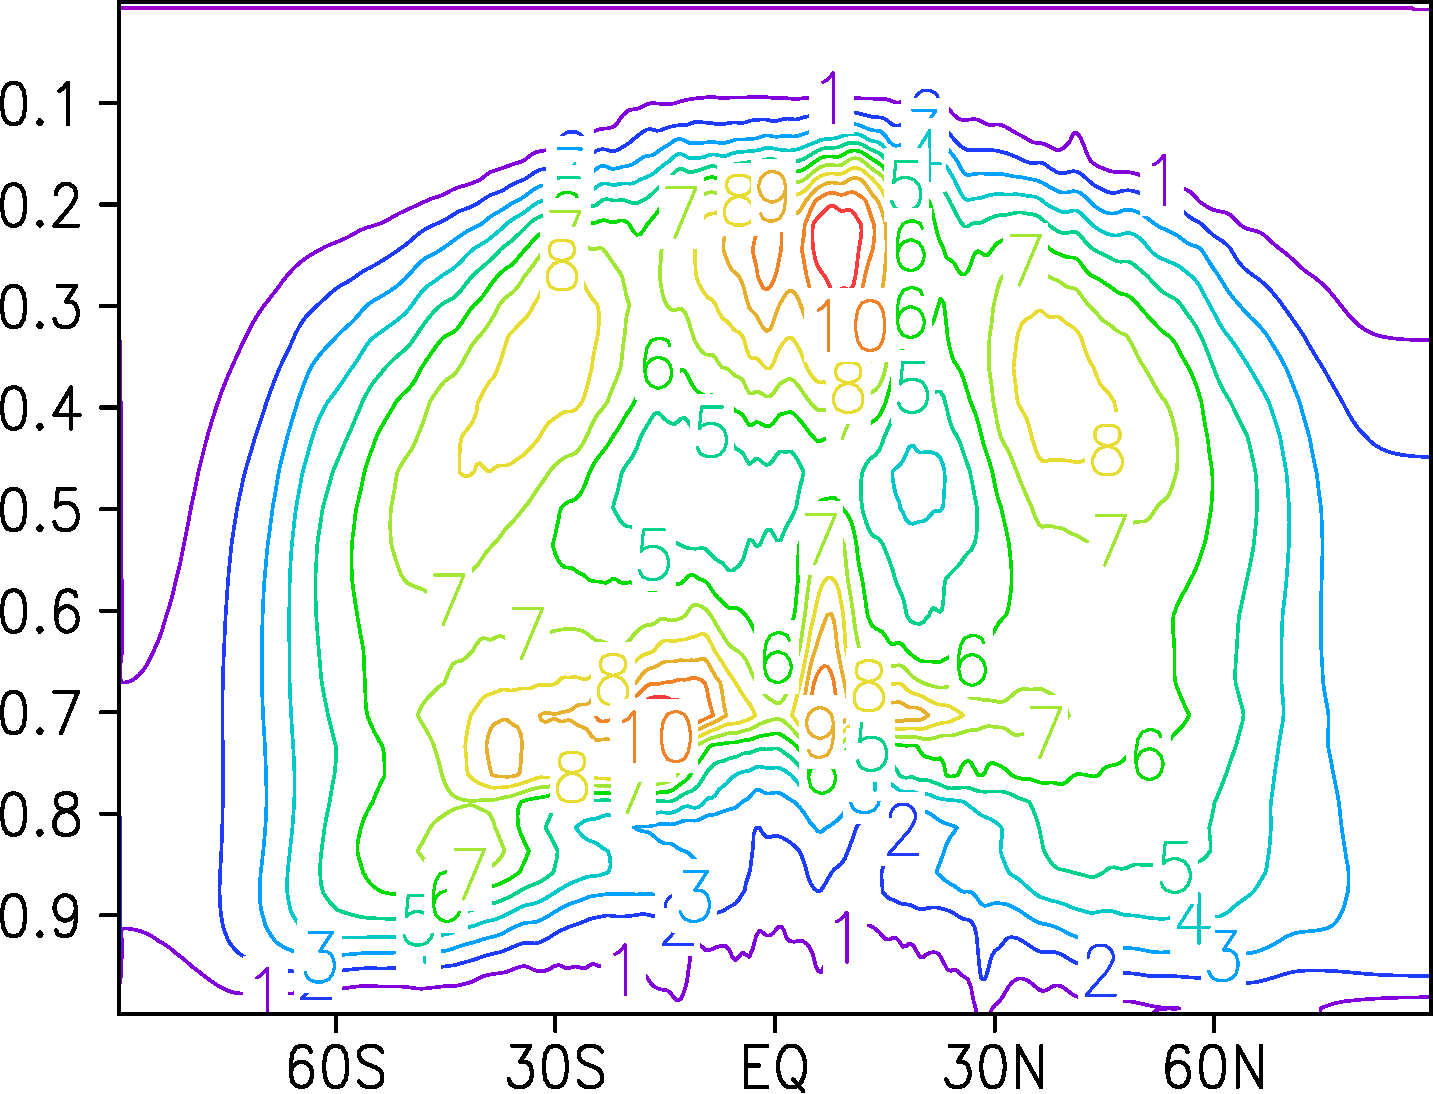
\includegraphics[width=0.3\textwidth,angle=0]{./figs/cap3/amplitudes_novas/amplitudes-NCEP_cw-orig-crop-rotated270.pdf}
        }   
    \end{center}
  \vspace{2mm}
  \legenda{}
  \label{fig:B_mcgav4_oz_cw}
  \FONTE{Produção do autor.}
\end{figure}

Nas Tabelas \ref{tab:amplimaxminB}, \ref{tab:comphorizmaxminB} e \ref{tab:compvertmaxminB} são apresentados os valores máximos e mínimos das quantidades apresentadas nas Figuras \ref{fig:B_mcgav4_psi}, \ref{fig:B_mcgav4_chi}, \ref{fig:B_mcgav4_T}, \ref{fig:B_mcgav4_q}, \ref{fig:B_mcgav4_ps} e \ref{fig:B_mcgav4_oz_cw} em adição as amplitudes e comprimentos de escalas da temperatura da superfície do mar.

\begin{table}[H]
\caption{Valores máximos e mínimos das amplitudes das versões das matrizes de covariâncias do CPTEC na resolução TQ0299L064 a partir dos pares de previsões de 48 e 24 horas do modelo MCGAv4.}
\begin{center}
\begin{adjustbox}{max width=\textwidth}
\begin{tabular}{ccccccccccccc}
\toprule
\toprule
\multicolumn{1}{c}{} & \multicolumn{2}{c}{\textbf{Bncep}} & \multicolumn{2}{c}{\textbf{Bcptec}} & \multicolumn{2}{c}{\textbf{B00Zcptec}} &\multicolumn{2}{c}{\textbf{B06Zcptec}} & \multicolumn{2}{c}{\textbf{B12Zcptec}} & \multicolumn{2}{c}{\textbf{B18Zcptec}} \\
\cmidrule(lr){2-3} \cmidrule(lr){4-5} \cmidrule(lr){6-7} \cmidrule(lr){8-9} \cmidrule(lr){10-11} \cmidrule(lr){12-13} 
\multicolumn{1}{c}{} & \multicolumn{1}{c}{\textbf{Máx}} & \multicolumn{1}{c}{\textbf{Mín}} & \multicolumn{1}{c}{\textbf{Máx}} & \multicolumn{1}{c}{\textbf{Mín}} & \multicolumn{1}{c}{\textbf{Máx}} & \multicolumn{1}{c}{\textbf{Mín}} & \multicolumn{1}{c}{\textbf{Máx}} & \multicolumn{1}{c}{\textbf{Mín}} & \multicolumn{1}{c}{\textbf{Máx}} & \multicolumn{1}{c}{\textbf{Mín}} & \multicolumn{1}{c}{\textbf{Máx}} & \multicolumn{1}{c}{\textbf{Mín}} \\
\midrule   
\multicolumn{1}{c}{$\psi$} & \multicolumn{1}{c}{7,99x$10^{6}$} & \multicolumn{1}{c}{4,3x$10^{5}$} & \multicolumn{1}{c}{2,8x$10^{7}$} & \multicolumn{1}{c}{4,6x$10^{5}$} & \multicolumn{1}{c}{1,7x$10^{7}$} & \multicolumn{1}{c}{4,9x$10^{5}$} & \multicolumn{1}{c}{1,9x$10^{7}$} & \multicolumn{1}{c}{4,9x$10^{5}$} & \multicolumn{1}{c}{1,7x$10^{7}$} & \multicolumn{1}{c}{4,9x$10^{5}$} & \multicolumn{1}{c}{1,7x$10^{7}$} & \multicolumn{1}{c}{4,8x$10^{5}$}  \\ 
\multicolumn{1}{c}{$\chi$} & \multicolumn{1}{c}{3,77x$10^{6}$} & \multicolumn{1}{c}{0} & \multicolumn{1}{c}{1,07x$10^{7}$} & \multicolumn{1}{c}{0} & \multicolumn{1}{c}{4,52x$10^{6}$} & \multicolumn{1}{c}{0} & \multicolumn{1}{c}{3,74x$10^{6}$} & \multicolumn{1}{c}{0} & \multicolumn{1}{c}{4,19x$10^{6}$} & \multicolumn{1}{c}{0} & \multicolumn{1}{c}{4,94x$10^{6}$} & \multicolumn{1}{c}{0} \\ 
\multicolumn{1}{c}{$T$}    & \multicolumn{1}{c}{2,23} & \multicolumn{1}{c}{0} & \multicolumn{1}{c}{4,04} & \multicolumn{1}{c}{0} & \multicolumn{1}{c}{3,01} & \multicolumn{1}{c}{0} & \multicolumn{1}{c}{3,11} & \multicolumn{1}{c}{0} & \multicolumn{1}{c}{3,13} & \multicolumn{1}{c}{0} & \multicolumn{1}{c}{3,03} & \multicolumn{1}{c}{0} \\ 
\multicolumn{1}{c}{$q$}    & \multicolumn{1}{c}{0,41} & \multicolumn{1}{c}{-4,06x$10^{-7}$} & \multicolumn{1}{c}{0,29} & \multicolumn{1}{c}{-2,15x$10^{-7}$} & \multicolumn{1}{c}{0,3} & \multicolumn{1}{c}{-2,12x$10^{-7}$} & \multicolumn{1}{c}{0,3} & \multicolumn{1}{c}{-2,27x$10^{-7}$} & \multicolumn{1}{c}{0,3} & \multicolumn{1}{c}{-2,59x$10^{-7}$} & \multicolumn{1}{c}{0,3} & \multicolumn{1}{c}{-2,53x$10^{-7}$} \\ 
\multicolumn{1}{c}{$oz$}  & \multicolumn{1}{c}{6,4x$10^{-7}$} & \multicolumn{1}{c}{-4,38x$10^{-7}$} & \multicolumn{1}{c}{4,4x$10^{-7}$} & \multicolumn{1}{c}{-2,2x$10^{-7}$} & \multicolumn{1}{c}{6,4x$10^{-7}$} & \multicolumn{1}{c}{-2,30x$10^{-7}$} & \multicolumn{1}{c}{6,4x$10^{-7}$} & \multicolumn{1}{c}{-2,33x$10^{-7}$} & \multicolumn{1}{c}{6,4x$10^{-7}$} & \multicolumn{1}{c}{-2,59x$10^{-7}$} & \multicolumn{1}{c}{6,4x$10^{-7}$} & \multicolumn{1}{c}{-2,63x$10^{-7}$} \\ 
\multicolumn{1}{c}{$cw$}  & \multicolumn{1}{c}{1,24x$10^{-4}$} & \multicolumn{1}{c}{-4,4x$10^{-7}$} & \multicolumn{1}{c}{1,24x$10^{-4}$} & \multicolumn{1}{c}{-2,4x$10^{-7}$} & \multicolumn{1}{c}{1,24x$10^{-4}$} & \multicolumn{1}{c}{-2,3x$10^{-7}$} & \multicolumn{1}{c}{1,24x$10^{-4}$} & \multicolumn{1}{c}{-2,33x$10^{-7}$} & \multicolumn{1}{c}{1,24x$10^{-4}$} & \multicolumn{1}{c}{-2,59x$10^{-7}$} & \multicolumn{1}{c}{1,24x$10^{-4}$} & \multicolumn{1}{c}{-2,64x$10^{-7}$} \\ 
\multicolumn{1}{c}{$ps$}   & \multicolumn{1}{c}{1,01x$10^{-1}$} & \multicolumn{1}{c}{4,88x$10^{-2}$} & \multicolumn{1}{c}{1,48x$10^{-1}$} & \multicolumn{1}{c}{6,35x$10^{-2}$} & \multicolumn{1}{c}{1,4x$10^{-1}$} & \multicolumn{1}{c}{5,27x$10^{-2}$} & \multicolumn{1}{c}{1,54x$10^{-1}$} & \multicolumn{1}{c}{5,43x$10^{-2}$} & \multicolumn{1}{c}{1,4x$10^{-1}$} & \multicolumn{1}{c}{5,48x$10^{-2}$} & \multicolumn{1}{c}{1,5x$10^{-1}$} & \multicolumn{1}{c}{5,48x$10^{-2}$} \\ 
\multicolumn{1}{c}{$sst$} & \multicolumn{1}{c}{4,32x$10^{-1}$} & \multicolumn{1}{c}{2x$10^{-1}$} & \multicolumn{1}{c}{4,32x$10^{-1}$} & \multicolumn{1}{c}{2x$10^{-1}$} & \multicolumn{1}{c}{4,32x$10^{-1}$} & \multicolumn{1}{c}{2x$10^{-1}$} & \multicolumn{1}{c}{4,32x$10^{-1}$} & \multicolumn{1}{c}{2x$10^{-1}$} & \multicolumn{1}{c}{4,32x$10^{-1}$} & \multicolumn{1}{c}{2x$10^{-1}$} & \multicolumn{1}{c}{4,32x$10^{-1}$} & \multicolumn{1}{c}{2x$10^{-1}$} \\ 
\bottomrule
\end{tabular}
\end{adjustbox}
\end{center}
\label{tab:amplimaxminB}
\end{table}

\begin{table}[H]
\caption{Idem Tabela \ref{tab:amplimaxminB}, para os comprimentos de escala horizontais.}
\begin{center}
\begin{adjustbox}{max width=\textwidth}
\begin{tabular}{ccccccccccccc}
\toprule
\toprule
\multicolumn{1}{c}{} & \multicolumn{2}{c}{\textbf{Bncep}} & \multicolumn{2}{c}{\textbf{Bcptec}} & \multicolumn{2}{c}{\textbf{B00Zcptec}} &\multicolumn{2}{c}{\textbf{B06Zcptec}} & \multicolumn{2}{c}{\textbf{B12Zcptec}} & \multicolumn{2}{c}{\textbf{B18Zcptec}} \\
\cmidrule(lr){2-3} \cmidrule(lr){4-5} \cmidrule(lr){6-7} \cmidrule(lr){8-9} \cmidrule(lr){10-11} \cmidrule(lr){12-13}
\multicolumn{1}{c}{} & \multicolumn{1}{c}{\textbf{Máx}} & \multicolumn{1}{c}{\textbf{Mín}} & \multicolumn{1}{c}{\textbf{Máx}} & \multicolumn{1}{c}{\textbf{Mín}} & \multicolumn{1}{c}{\textbf{Máx}} & \multicolumn{1}{c}{\textbf{Mín}} & \multicolumn{1}{c}{\textbf{Máx}} & \multicolumn{1}{c}{\textbf{Mín}} & \multicolumn{1}{c}{\textbf{Máx}} & \multicolumn{1}{c}{\textbf{Mín}} & \multicolumn{1}{c}{\textbf{Máx}} & \multicolumn{1}{c}{\textbf{Mín}} \\
\midrule
\multicolumn{1}{c}{$\psi$} & \multicolumn{1}{c}{1,3x$10^{6}$} & \multicolumn{1}{c}{2,2x$10^{5}$} & \multicolumn{1}{c}{1,75x$10^{6}$} & \multicolumn{1}{c}{4,55x$10^{5}$} & \multicolumn{1}{c}{1,32x$10^{6}$} & \multicolumn{1}{c}{4,73x$10^{5}$} & \multicolumn{1}{c}{1,4x$10^{6}$} & \multicolumn{1}{c}{4,7x$10^{5}$} & \multicolumn{1}{c}{1,31x$10^{6}$} & \multicolumn{1}{c}{4,7x$10^{5}$} & \multicolumn{1}{c}{1,27x$10^{6}$} & \multicolumn{1}{c}{4,73x$10^{5}$} \\ 
\multicolumn{1}{c}{$\chi$} & \multicolumn{1}{c}{1,1x$10^{6}$} & \multicolumn{1}{c}{0} & \multicolumn{1}{c}{1,82x$10^{6}$} & \multicolumn{1}{c}{0} & \multicolumn{1}{c}{1,37x$10^{6}$} & \multicolumn{1}{c}{0} & \multicolumn{1}{c}{1,45x$10^{6}$} & \multicolumn{1}{c}{0} & \multicolumn{1}{c}{1,5x$10^{6}$} & \multicolumn{1}{c}{0} & \multicolumn{1}{c}{1,42x$10^{6}$} & \multicolumn{1}{c}{0} \\ 
\multicolumn{1}{c}{$T$}    & \multicolumn{1}{c}{3,1x$10^{5}$} & \multicolumn{1}{c}{0} & \multicolumn{1}{c}{5,9x$10^{5}$} & \multicolumn{1}{c}{0} & \multicolumn{1}{c}{5,94x$10^{5}$} & \multicolumn{1}{c}{0} & \multicolumn{1}{c}{5,9x$10^{5}$} & \multicolumn{1}{c}{0} & \multicolumn{1}{c}{6,42x$10^{5}$} & \multicolumn{1}{c}{0} & \multicolumn{1}{c}{6,37x$10^{5}$} & \multicolumn{1}{c}{0} \\ 
\multicolumn{1}{c}{$q$}    & \multicolumn{1}{c}{7,9x$10^{6}$} & \multicolumn{1}{c}{0} & \multicolumn{1}{c}{2,22x$10^{7}$} & \multicolumn{1}{c}{0} & \multicolumn{1}{c}{1,31x$10^{7}$} & \multicolumn{1}{c}{0} & \multicolumn{1}{c}{1,48x$10^{7}$} & \multicolumn{1}{c}{0} & \multicolumn{1}{c}{1,33x$10^{7}$} & \multicolumn{1}{c}{0} & \multicolumn{1}{c}{1,36x$10^{7}$} & \multicolumn{1}{c}{0} \\ 
\multicolumn{1}{c}{$oz$}   & \multicolumn{1}{c}{7,99x$10^{6}$} & \multicolumn{1}{c}{0} & \multicolumn{1}{c}{2,84x$10^{7}$} & \multicolumn{1}{c}{0} & \multicolumn{1}{c}{1,73x$10^{7}$} & \multicolumn{1}{c}{0} & \multicolumn{1}{c}{1,96x$10^{7}$} & \multicolumn{1}{c}{0} & \multicolumn{1}{c}{1,75x$10^{7}$} & \multicolumn{1}{c}{0} & \multicolumn{1}{c}{1,78x$10^{7}$} & \multicolumn{1}{c}{0} \\ 
\multicolumn{1}{c}{$cw$}   & \multicolumn{1}{c}{7,99x$10^{6}$} & \multicolumn{1}{c}{0} & \multicolumn{1}{c}{2,84x$10^{7}$} & \multicolumn{1}{c}{0} & \multicolumn{1}{c}{1,73x$10^{7}$} & \multicolumn{1}{c}{0} & \multicolumn{1}{c}{1,96x$10^{7}$} & \multicolumn{1}{c}{0} & \multicolumn{1}{c}{1,75x$10^{7}$} & \multicolumn{1}{c}{0} & \multicolumn{1}{c}{1,78x$10^{7}$} & \multicolumn{1}{c}{0} \\ 
\multicolumn{1}{c}{$ps$}   & \multicolumn{1}{c}{1,89x$10^{5}$} & \multicolumn{1}{c}{1,19x$10^{5}$} & \multicolumn{1}{c}{4,18x$10^{5}$} & \multicolumn{1}{c}{1,83x$10^{5}$} & \multicolumn{1}{c}{3,9x$10^{5}$} & \multicolumn{1}{c}{1,83x$10^{5}$} & \multicolumn{1}{c}{3,9x$10^{5}$} & \multicolumn{1}{c}{1,8x$10^{5}$} & \multicolumn{1}{c}{3,8x$10^{5}$} & \multicolumn{1}{c}{1,8x$10^{5}$} & \multicolumn{1}{c}{3,9x$10^{5}$} & \multicolumn{1}{c}{1,84x$10^{5}$} \\ 
\multicolumn{1}{c}{$sst$}  & \multicolumn{1}{c}{8x$10^{2}$} & \multicolumn{1}{c}{5,07x$10^{2}$} & \multicolumn{1}{c}{8x$10^{2}$} & \multicolumn{1}{c}{5,07x$10^{2}$} & \multicolumn{1}{c}{8x$10^{2}$} & \multicolumn{1}{c}{5,07x$10^{2}$} & \multicolumn{1}{c}{8x$10^{2}$} & \multicolumn{1}{c}{5,07x$10^{2}$} & \multicolumn{1}{c}{8x$10^{2}$} & \multicolumn{1}{c}{5,07x$10^{2}$} & \multicolumn{1}{c}{8x$10^{2}$} & \multicolumn{1}{c}{5,07x$10^{2}$} \\ 
\bottomrule
\end{tabular}
\end{adjustbox}
\end{center}
\label{tab:comphorizmaxminB}
\end{table}

\begin{table}[H]
\caption{Idem Tabela \ref{tab:amplimaxminB}, para os comprimentos de escala verticais.}
\begin{center}
\begin{adjustbox}{max width=\textwidth}
\begin{tabular}{ccccccccccccc}
\toprule
\toprule
\multicolumn{1}{c}{} & \multicolumn{2}{c}{\textbf{Bncep}} & \multicolumn{2}{c}{\textbf{Bcptec}} & \multicolumn{2}{c}{\textbf{B00Zcptec}} &\multicolumn{2}{c}{\textbf{B06Zcptec}} & \multicolumn{2}{c}{\textbf{B12Zcptec}} & \multicolumn{2}{c}{\textbf{B18Zcptec}} \\
\cmidrule(lr){2-3} \cmidrule(lr){4-5} \cmidrule(lr){6-7} \cmidrule(lr){8-9} \cmidrule(lr){10-11} \cmidrule(lr){12-13}
\multicolumn{1}{c}{} & \multicolumn{1}{c}{\textbf{Máx}} & \multicolumn{1}{c}{\textbf{Mín}} & \multicolumn{1}{c}{\textbf{Máx}} & \multicolumn{1}{c}{\textbf{Mín}} & \multicolumn{1}{c}{\textbf{Máx}} & \multicolumn{1}{c}{\textbf{Mín}} & \multicolumn{1}{c}{\textbf{Máx}} & \multicolumn{1}{c}{\textbf{Mín}} & \multicolumn{1}{c}{\textbf{Máx}} & \multicolumn{1}{c}{\textbf{Mín}} & \multicolumn{1}{c}{\textbf{Máx}} & \multicolumn{1}{c}{\textbf{Mín}} \\
\midrule
\multicolumn{1}{c}{$\psi$} & \multicolumn{1}{c}{9,1x$10^{-1}$} & \multicolumn{1}{c}{8,3x$10^{-2}$} & \multicolumn{1}{c}{1,27} & \multicolumn{1}{c}{8,41x$10^{-2}$} & \multicolumn{1}{c}{1,16} & \multicolumn{1}{c}{8,52x$10^{-2}$} & \multicolumn{1}{c}{1,27} & \multicolumn{1}{c}{8,59x$10^{-2}$} & \multicolumn{1}{c}{1,08} & \multicolumn{1}{c}{8,54x$10^{-2}$} & \multicolumn{1}{c}{1,17} & \multicolumn{1}{c}{8,54x$10^{-2}$} \\ 
\multicolumn{1}{c}{$\chi$} & \multicolumn{1}{c}{1,22} & \multicolumn{1}{c}{0} & \multicolumn{1}{c}{1,5} & \multicolumn{1}{c}{0} & \multicolumn{1}{c}{1,85} & \multicolumn{1}{c}{0} & \multicolumn{1}{c}{1,74} & \multicolumn{1}{c}{0} & \multicolumn{1}{c}{1,78} & \multicolumn{1}{c}{0} & \multicolumn{1}{c}{1,65} & \multicolumn{1}{c}{0} \\ 
\multicolumn{1}{c}{$T$}    & \multicolumn{1}{c}{1,75} & \multicolumn{1}{c}{0} & \multicolumn{1}{c}{1,67} & \multicolumn{1}{c}{0} & \multicolumn{1}{c}{1,68} & \multicolumn{1}{c}{0} & \multicolumn{1}{c}{1,63} & \multicolumn{1}{c}{0} & \multicolumn{1}{c}{1,62} & \multicolumn{1}{c}{0} & \multicolumn{1}{c}{1,68} & \multicolumn{1}{c}{0} \\ 
\multicolumn{1}{c}{$q$}    & \multicolumn{1}{c}{1,3x$10^{6}$} & \multicolumn{1}{c}{0} & \multicolumn{1}{c}{1,75x$10^{6}$} & \multicolumn{1}{c}{0} & \multicolumn{1}{c}{1,28x$10^{6}$} & \multicolumn{1}{c}{0} & \multicolumn{1}{c}{1,33x$10^{6}$} & \multicolumn{1}{c}{0} & \multicolumn{1}{c}{1,27x$10^{6}$} & \multicolumn{1}{c}{0} & \multicolumn{1}{c}{1,23x$10^{6}$} & \multicolumn{1}{c}{0} \\ 
\multicolumn{1}{c}{$oz$}   & \multicolumn{1}{c}{1,3x$10^{6}$} & \multicolumn{1}{c}{0} & \multicolumn{1}{c}{1,82x$10^{6}$} & \multicolumn{1}{c}{0} & \multicolumn{1}{c}{1,37x$10^{6}$} & \multicolumn{1}{c}{0} & \multicolumn{1}{c}{1,45x$10^{6}$} & \multicolumn{1}{c}{0} & \multicolumn{1}{c}{1,47x$10^{6}$} & \multicolumn{1}{c}{0} & \multicolumn{1}{c}{1,42x$10^{6}$} & \multicolumn{1}{c}{0} \\ 
\multicolumn{1}{c}{$cw$}   & \multicolumn{1}{c}{1,3x$10^{6}$} & \multicolumn{1}{c}{0} & \multicolumn{1}{c}{1,82x$10^{6}$} & \multicolumn{1}{c}{0} & \multicolumn{1}{c}{1,37x$10^{6}$} & \multicolumn{1}{c}{0} & \multicolumn{1}{c}{1,45x$10^{6}$} & \multicolumn{1}{c}{0} & \multicolumn{1}{c}{1,47x$10^{6}$} & \multicolumn{1}{c}{0} & \multicolumn{1}{c}{1,42x$10^{6}$} & \multicolumn{1}{c}{0} \\ 
%\multicolumn{1}{c}{$ps$}   & \multicolumn{1}{c}{} & \multicolumn{1}{c}{} & \multicolumn{1}{c}{} & \multicolumn{1}{c}{} & \multicolumn{1}{c}{} & \multicolumn{1}{c}{} & \multicolumn{1}{c}{} & \multicolumn{1}{c}{} & \multicolumn{1}{c}{} & \multicolumn{1}{c}{} & \multicolumn{1}{c}{} & \multicolumn{1}{c}{} \\ 
%\multicolumn{1}{c}{$sst$}  & \multicolumn{1}{c}{} & \multicolumn{1}{c}{} & \multicolumn{1}{c}{} & \multicolumn{1}{c}{} & \multicolumn{1}{c}{} & \multicolumn{1}{c}{} & \multicolumn{1}{c}{} & \multicolumn{1}{c}{} & \multicolumn{1}{c}{} & \multicolumn{1}{c}{} & \multicolumn{1}{c}{} & \multicolumn{1}{c}{} \\ 
\bottomrule
\end{tabular}
\end{adjustbox}
\end{center}
\label{tab:compvertmaxminB}
\end{table}

% \section{Testes de Sensibilidade}

% Na literatura, os estudos que incluíram o cálculo da matriz de covariâncias para um determinado sistema a fim de ser aplicada ao estudo de fenômenos em diferentes escalas espaciais e temporais, por muitas vezes, não discutem com clareza dois importantes aspectos para o cálculo da matriz de covariâncias: i) a quantidade de pares de previsões utilizados; ii) a sua distribuição ou escala temporal. Estes dois aspectos são mencionados em eg., \citeonline{wuetal/2002} onde é citado o uso de 49 pares de previsões de 48 e 24 horas distribuídos ao longo de 1 ano. A partir desta afirmação, é possível formular as seguintes perguntas: a) qual seria um número mínimo de pares de previsões para o cálculo de uma matriz de covariâncias para uso operacional em um sistema de baixa resolução horizontal e vertical (eg., TQ0062L028)? b) uma vez estabelecida a hipótese ``a'', a próxima questão seria b) o mesmo é válido para resoluções diferentes (eg., TQ0299L064)? c) qual seria a distribuição temporal adequada dos pares de previsões ao longo de 1 ano? Estes pares possuem distribuição linear (ie., são igualmente espaçados) ou a sua distribuição deve ser sazonal (i.e., mais ou menos concentrada em determinadas estações)?.

% Dado que a componente dinâmica do sistema híbrido é realizada por um sistema baseado em conjuntos, estas questões serão testadas utilizando-se a componente estacionária do sistema. Da mesma forma, pode-se especular que a componente dinâmica do sistema híbrido também possa ser testada da mesma maneira. Por outro lado, deve-se considerar também a hipótese de que apenas conjunto de previsões tendendo ao infinito será capaz de fornecer uma matriz de covariâncias com posto completo (ie., \textit{full rank}).

% \subsection*{Número de Pares de Previsões}

% Os testes com o número de pares de previsões foram realizados considerando-se as seguintes configurações:

% TABELA COM OS NUMEROS DE PARES E RESOLUÇÔES E PERIODOS. \improvement{aproveitar algumas figuras que fiz variando pares de previsões; estas figuras estão na Wiki Berror.}

% Para que seja possível definir um limite a fim de se afirmar se a diferença entre as matrizes é significativa ou não, foram estabelecidos os seguintes critérios:

% \begin{itemize}
% \item Diferença na função de corrente menor do que X; \improvement{aqui posso incluir as figuras de ``dispersão'' que eu fiz, comparando as matrizes por regiões e verificando onde está a maior correlação entre elas.}
% \item ...
% \end{itemize}

% \subsection*{Escala Temporal}

% Os testes de sensibilidade na escala temporal visam estabelecer como os pares de uma matriz de covariâncias deficiente em posto (ie., \textit{rank defficient}) são distribuídos ao longo do tempo e de que maneira esta distribuição afeta a qualidade dos incrementos de análise.

% \subsection*{Escala Espacial}

% Nesta seção serão apresentadas as características principais do incremento de análise quando são variados os parâmetros espaciais da matriz de covariâncias. Para este propósito, foram realizados uma séries de experimentos com observação única (na resolução TQ0062L028), entre os quais foram considerados os seguintes parâmetros:

% \subsubsection*{Parâmetros relacionados à Observação:}

% \begin{itemize}
%     \item \textbf{maginnov:} magnitude da inovação da observação;
%     \item \textbf{magoberr:} magnitude do erro da observação;
% \end{itemize}

% \subsubsection*{Parâmetros relacionados à Matriz de Covariâncias:}

% \begin{itemize}
%     \item \textbf{vs:} fator de escalonamento para o comprimento de correlação vertical do erro de previsão;
%     \item \textbf{hzscl:} fator de escalonamento para suavização horizontal;
%     \item \textbf{hswgt:} pesos empíricos a serem aplicados a cada fator de escalonamento horizontal;
%     \item \textbf{bw:} fator no cálculo do erro de previsão;
%     \item \textbf{bkg\_flowdep:} flag para habilitar a dependência do fluxo nas variâncias do erro de previsão;
%     \item \textbf{bkg\_rewgfct:} fator usado para realizar o reponderamento das variâncias do erro dependentes do fluxo.
% \end{itemize}

% Nos experimentos com observação única, foram ajustados os seguintes parâmetros, dos quais, os valores padrão estão sumarizados na tabela a seguir:\fazer{refazer figuras e selecionar aquelas que são mais significativas.}

% \begin{table}[!h]
% \caption{Tabela com os valores padrão das configurações do Experimento com Observação Única.}
% \begin{center}
% \begin{adjustbox}{max width=\textwidth}
% %\renewcommand{\arraystretch}{1.5}
% \begin{tabular}{lll}
% \toprule
% \toprule
% \textbf{BKGERR}       & \textbf{ANBKGERR}   & \textbf{SINGLEOB\_TEST} \\
% \midrule
% vs=0.7                & maginnov=1.0        & anisotropic=false       \\
% hzscl=1.7, 0.8, 0.5   & magoberr=1.0        & covmap=false            \\
% hswgt=0.45, 0.3, 0.25 & oneob\_type=t       &              ~          \\
% bw=0.0                & oblat=20            &              ~          \\
% norsp=4               & oblon=285           &              ~          \\
% bkgv\_flowdep=false   & obpres=850          &              ~          \\
% bkgv\_rewgtfct=1.5    & obdattim=2013010100 &              ~          \\
%               ~      & obhourset=0         &              ~          \\  
% \bottomrule
% \end{tabular}
% \end{adjustbox}
% \end{center}
% \label{tab:sensitest}
% \end{table}

% \begin{figure}[!h]
%     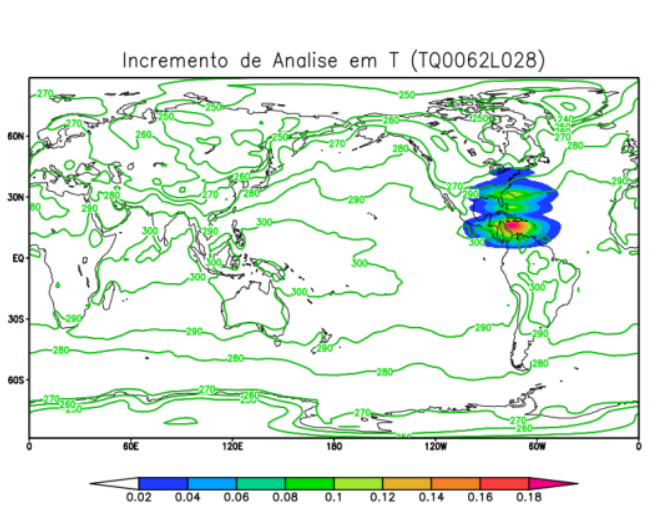
\includegraphics[width=8cm]{./figs/cap3/t_lat_lon-ref.png}
%     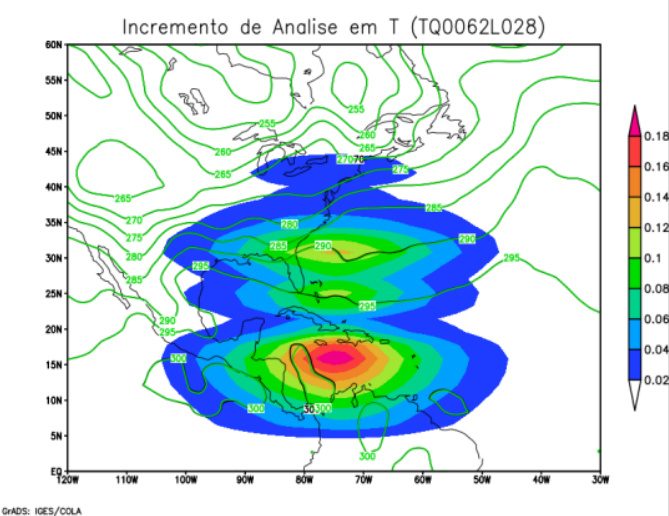
\includegraphics[width=8cm]{./figs/cap3/t_lat_lon-ref_zoom.png}
%     \\
%     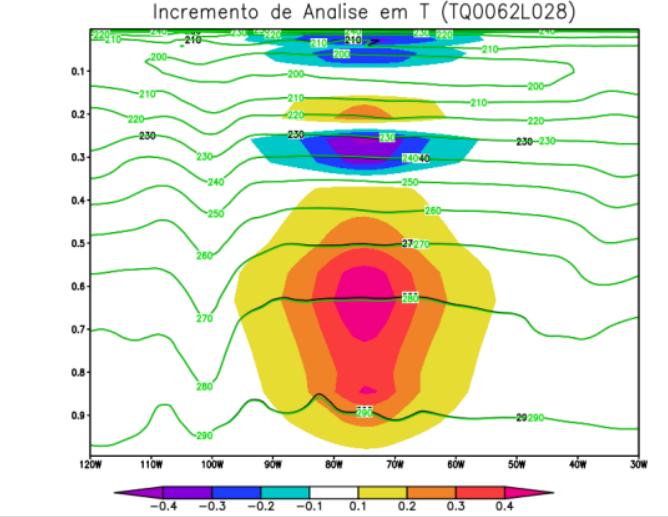
\includegraphics[width=8cm]{./figs/cap3/t_sig_lon-ref.png}
%     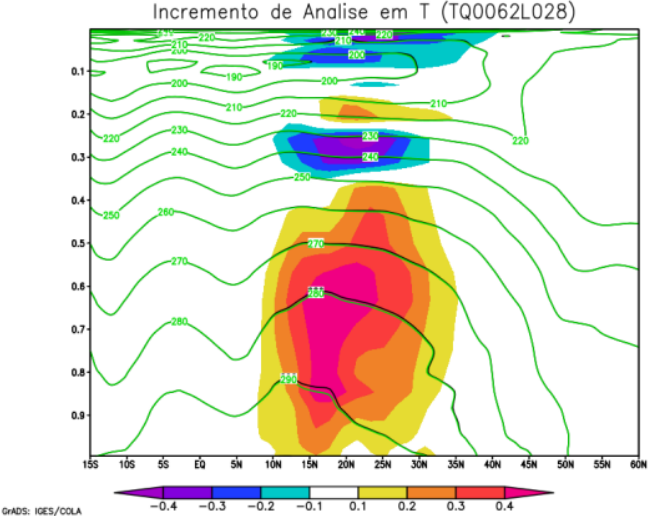
\includegraphics[width=8cm]{./figs/cap3/t_sig_lat-ref.png}
% \end{figure}

% \newpage

\subsection{Correlações entre B CPTEC X NCEP}
\label{sec:simi_B-cptec_ncep}

Aproveitando-se do fato de que a matriz de covariâncias do CPTEC na resolução TQ0299L064 utilizando os pares de previsões de 48 e 24 horas do MCGAv4 foi calculada com dimensões de grade iguais as da matriz de covariâncias do NCEP, então é possível fazer uma comparação direta. A matriz de covariâncias global do NCEP - e que esteve em uso por um breve período na operação do sistema G3DVAR (v1.1.3) no CPTEC, foi calculada com base nos pares de previsões do modelo GFS. Ambos os modelos, MCGAv4 e GFS, são modelos espectrais e as mesmas variáveis foram utilizadas para o cálculo das matrizes de covariâncias. A comparação entre as duas matrizes foi feita a partir do diagrama de espalhamento considerando a distribuição das médias latitudinais nos 64 níveis de cada variável. Nas comparações feitas a seguir, foram consideradas as variáveis $\psi$, $\chi$, $T$ e $q$ nas regiões Hemisfério Norte (HN - lons: 0-360; lats:20N-80N), Trópicos (TR - lons:0-360; lats:20S-20N) e Hemisfério Sul (HS - lons:0-360; lats: 80S-20S). O particionamento em regiões para esta comparação, tem como objetivo melhorar a identificação das correlações entre as variáveis indicadas. Para cada figura, foram calculadas a curva de ajuste, o erro quadrático ($r^{2}$) e o coeficiente de correlação de Pearson ($r$).

Na Figura \ref{fig:disper_Allz_hn_tr_hs}, são apresentados diagramas de dispersão entre as matrizes de covariâncias do NCEP e CPTEC (todos os horários, AllZ), para as variáveis $\psi$, $\chi$, $T$ e $q$, sobre as regiões HN, TR e HS. Em geral, a correlação entre as quantidades consideradas das duas matrizes de covariâncias apresentam valores em torno de 0,9 (90\%), o que reflete as semelhanças encontradas nas amplitudes apresentadas na seção anterior. Além disso, maiores correlações foram encontradas sobre o Hemisfério Sul, enquanto que sobre a região Tropical, foram encontradas as menores correlações. As variáveis que possuem a maior correlação são a função de corrente ($\psi$) e a velocidade potencial ($\chi$) sobre o Hemisfério Sul (Figuras \ref{fig:disper_sfAllz_sh} e \ref{fig:disper_vpAllz_sh}). Entretanto, verificou-se também que as amplitudes de $q$ apresentam os menores valores de correlação e maior erro nos níveis mais altos do modelo. Isto indica que há uma discrepância na representação da umidade a partir do nível 22 (nível sigma 0,604374, aproximadamente 618,88 hPa) até o topo do modelo sobre o Hemisfério Norte. Sobre os Trópicos, as discrepâncias na representação das amplitudes da umidade, estão em níveis mais baixo. Para a umidade, a correlação sobre esta região é de 0,511 (aproximadamente 51\% - Figura \ref{fig:disper_qAllz_tr}). Entretanto, sobre o Hemisfério Sul, a correlação entre as amplitudes da umidade das duas matrizes é alta (aproximadamente 90\%). Sobre esta região, as maiores diferenças estão nos níveis médios. Nas Tabelas \ref{tab:disper_vals_BcptecXncep-sfvp} e \ref{tab:disper_vals_BcptecXncep-Tq}, estão sumarizados os valores de correlação e erro quadrático calculados para todos os horários sinóticos individuais. Neste caso, ressalta-se que as matrizes calculadas para os horários das 00, 06, 12 e 18Z, foram correlacionadas para as regiões indicadas com a matriz de covariâncias do NCEP.

\begin{table}[H]
\caption{Coeficiente de Correlação de Pearson ($r$) e Erro Quadrático ($r^{2}$) para as amplitudes de $\psi$ e $\chi$, entre as matrizes $\mathbf{B}$ CPTEC e NCEP (TQ0299L064) sobre as regiões HN, TR e HS e para os horários AllZ (todos) e 00Z, 06, 12Z e 18Z. Em vermelho, estão destacados os valores de correlação menores do que 0,9.}
\begin{center}
\begin{adjustbox}{max width=\textwidth}
\begin{tabular}{rcccccccccccc}
\toprule
\toprule
        & \multicolumn{6}{c}{$\psi$} & \multicolumn{6}{c}{$\chi$} \\
\cmidrule(lr{.75em}){2-7} \cmidrule(lr{.75em}){8-13}
        & \multicolumn{2}{c}{\textbf{HN}} & \multicolumn{2}{c}{\textbf{TR}} & \multicolumn{2}{c}{\textbf{HS}} & \multicolumn{2}{c}{\textbf{HN}} & \multicolumn{2}{c}{\textbf{TR}} & \multicolumn{2}{c}{\textbf{HS}} \\ 
\cmidrule(lr{.75em}){2-3} \cmidrule(lr{.75em}){4-5} \cmidrule(lr{.75em}){6-7} \cmidrule(lr{.75em}){8-9} \cmidrule(lr{.75em}){10-11} \cmidrule(lr{.75em}){12-13}   
           & $r$ & $r^{2}$ & $r$ & $r^{2}$ & $r$ & $r^{2}$ & $r$ & $r^{2}$ & $r$ & $r^{2}$ & $r$ & $r^{2}$\\ 
\midrule
\textbf{00Z}  & 0,972 & 0,945 & 0,925 & 0,855 & 0,953 & 0,908 & 0,979 & 0,959 & 0,977 & 0,955 & 0,972 & 0,946 \\
\textbf{06Z}  & 0,966 & 0,933 & 0,934 & 0,873 & 0,962 & 0,925 & 0,976 & 0,952 & 0,972 & 0,946 & 0,974 & 0,950 \\
\textbf{12Z}  & 0,975 & 0,951 & 0,940 & 0,885 & 0,963 & 0,927 & 0,978 & 0,956 & 0,977 & 0,955 & 0,970 & 0,941 \\
\textbf{18Z}  & 0,977 & 0,955 & 0,932 & 0,870 & 0,965 & 0,931 & 0,971 & 0,944 & 0,978 & 0,957 & 0,973 & 0,947 \\
\textbf{AllZ} & 0,958 & 0,918 & \textcolor{red}{0,828} & 0,686 & 0,989 & 0,979 & 0,947 & 0,897 & 0,921 & 0,848 & 0,965 & 0,932 \\
\bottomrule     
\end{tabular}
\end{adjustbox}
\end{center}
\label{tab:disper_vals_BcptecXncep-sfvp}
\end{table}

\begin{table}[H]
\caption{Idem Tabela \ref{tab:disper_vals_BcptecXncep-sfvp}, para as variáveis temperatura ($T$) e umidade ($q$).}
\begin{center}
\begin{adjustbox}{max width=\textwidth}
\begin{tabular}{rcccccccccccc}
\toprule
\toprule
        & \multicolumn{6}{c}{$T$} & \multicolumn{6}{c}{$q$} \\
\cmidrule(lr{.75em}){2-7} \cmidrule(lr{.75em}){8-13}
        & \multicolumn{2}{c}{\textbf{HN}} & \multicolumn{2}{c}{\textbf{TR}} & \multicolumn{2}{c}{\textbf{HS}} & \multicolumn{2}{c}{\textbf{HN}} & \multicolumn{2}{c}{\textbf{TR}} & \multicolumn{2}{c}{\textbf{HS}} \\ 
\cmidrule(lr{.75em}){2-3} \cmidrule(lr{.75em}){4-5} \cmidrule(lr{.75em}){6-7} \cmidrule(lr{.75em}){8-9} \cmidrule(lr{.75em}){10-11} \cmidrule(lr{.75em}){12-13}
           & $r$ & $r^{2}$ & $r$ & $r^{2}$ & $r$ & $r^{2}$ & $r$ & $r^{2}$ & $r$ & $r^{2}$ & $r$ & $r^{2}$\\ 
\midrule 
\textbf{00Z}  & 0,966 & 0,934 & 0,985 & 0,970 & 0,966 & 0,934 & \textcolor{red}{0,879} & 0,773 & \textcolor{red}{0,761} & 0,579 & 0,942 & 0,888 \\
\textbf{06Z}  & 0,965 & 0,932 & 0,983 & 0,967 & 0,963 & 0,928 & \textcolor{red}{0,878} & 0,771 & \textcolor{red}{0,761} & 0,579 & 0,945 & 0,893 \\
\textbf{12Z}  & 0,964 & 0,931 & 0,984 & 0,969 & 0,962 & 0,927 & \textcolor{red}{0,883} & 0,781 & \textcolor{red}{0,758} & 0,575 & 0,944 & 0,892 \\
\textbf{18Z}  & 0,966 & 0,935 & 0,985 & 0,971 & 0,965 & 0,932 & \textcolor{red}{0,881} & 0,777 & \textcolor{red}{0,756} & 0,572 & 0,945 & 0,893 \\
\textbf{AllZ} & 0,929 & 0,863 & 0,962 & 0,927 & 0,947 & 0,897 & \textcolor{red}{0,867} & 0,752 & \textcolor{red}{0,715} & 0,511 & 0,953 & 0,909 \\
\bottomrule                                        
\end{tabular}
\end{adjustbox}
\end{center}
\label{tab:disper_vals_BcptecXncep-Tq}
\end{table}

\begin{figure}[H]
    \vspace{-6mm}
    \caption{Diagramas de dispersão entre as amplitudes representadas nas matrizes de covariâncias $\mathbf{B}$ CPTEC e NCEP.}
    \begin{center}
        \subfigure[$\psi$ AllZ (HN)]{
            \label{fig:disper_sfAllz_hn}
            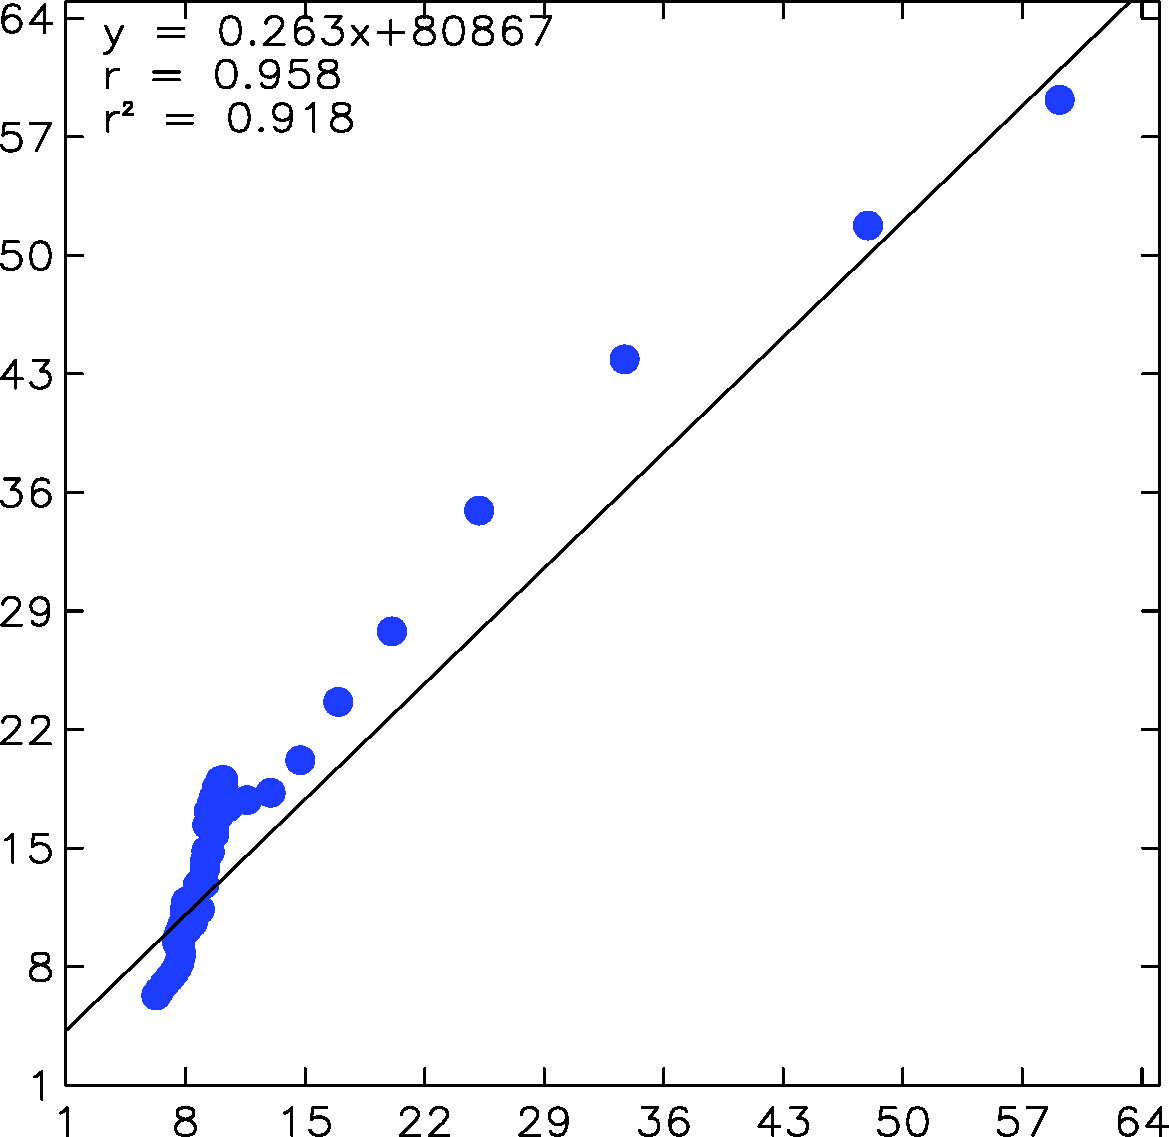
\includegraphics[width=0.3\textwidth,angle=0]{./figs/cap3/disper_novas/scatter-indiv_sf_NH_cptecAllZ_ncep-crop-rotated270.pdf}
        }
        \subfigure[$\psi$ AllZ (TR)]{
           \label{fig:disper_sfAllz_tr}
           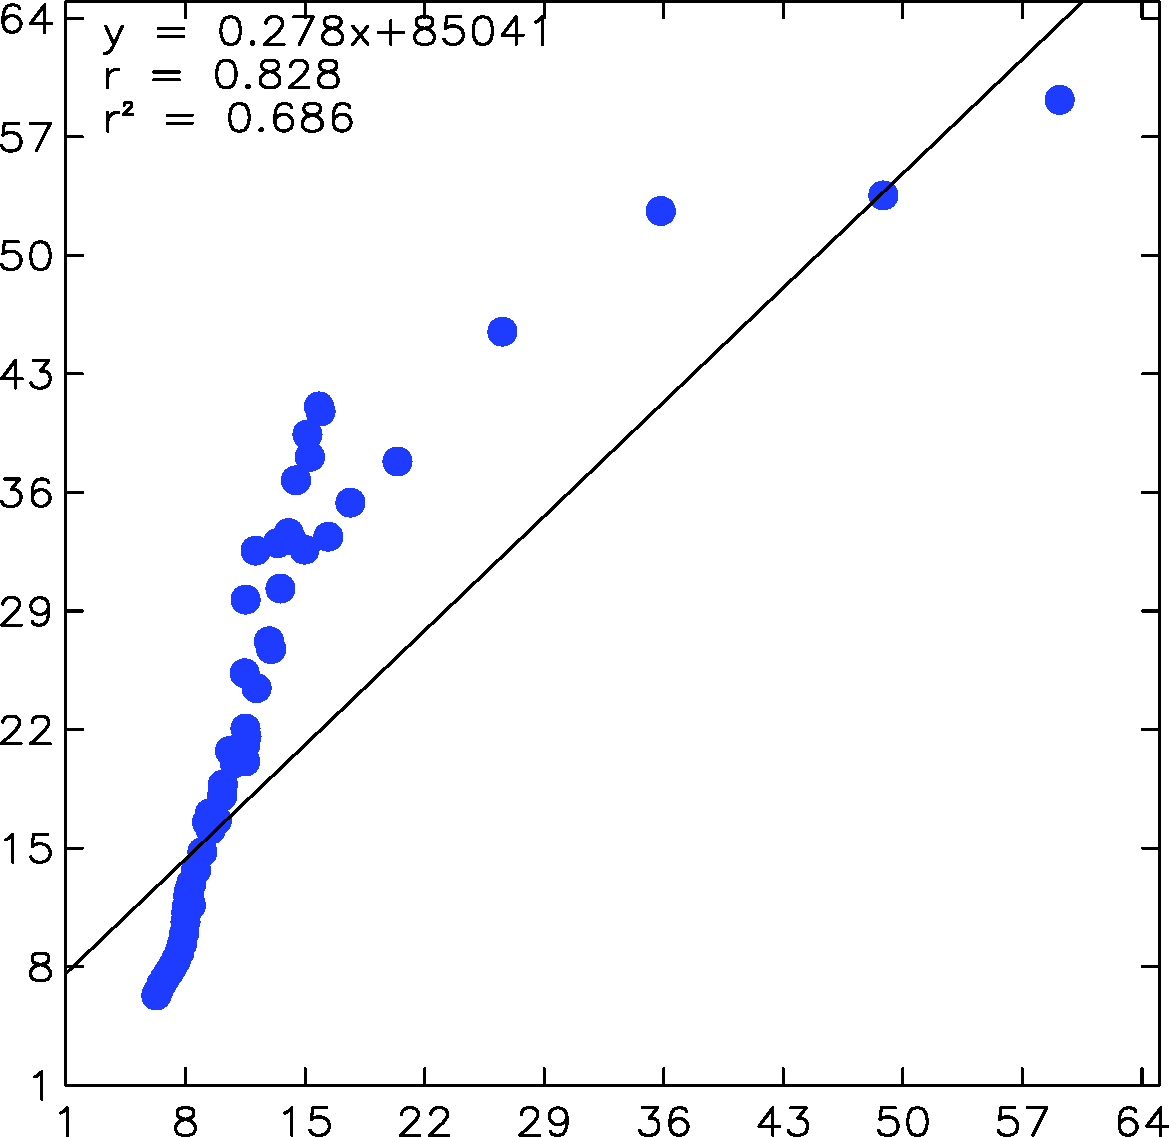
\includegraphics[width=0.3\textwidth,angle=0]{./figs/cap3/disper_novas/scatter-indiv_sf_TR_cptecAllZ_ncep-crop-rotated270.pdf}
        }
        \subfigure[$\psi$ AllZ (HS)]{
           \label{fig:disper_sfAllz_sh}
           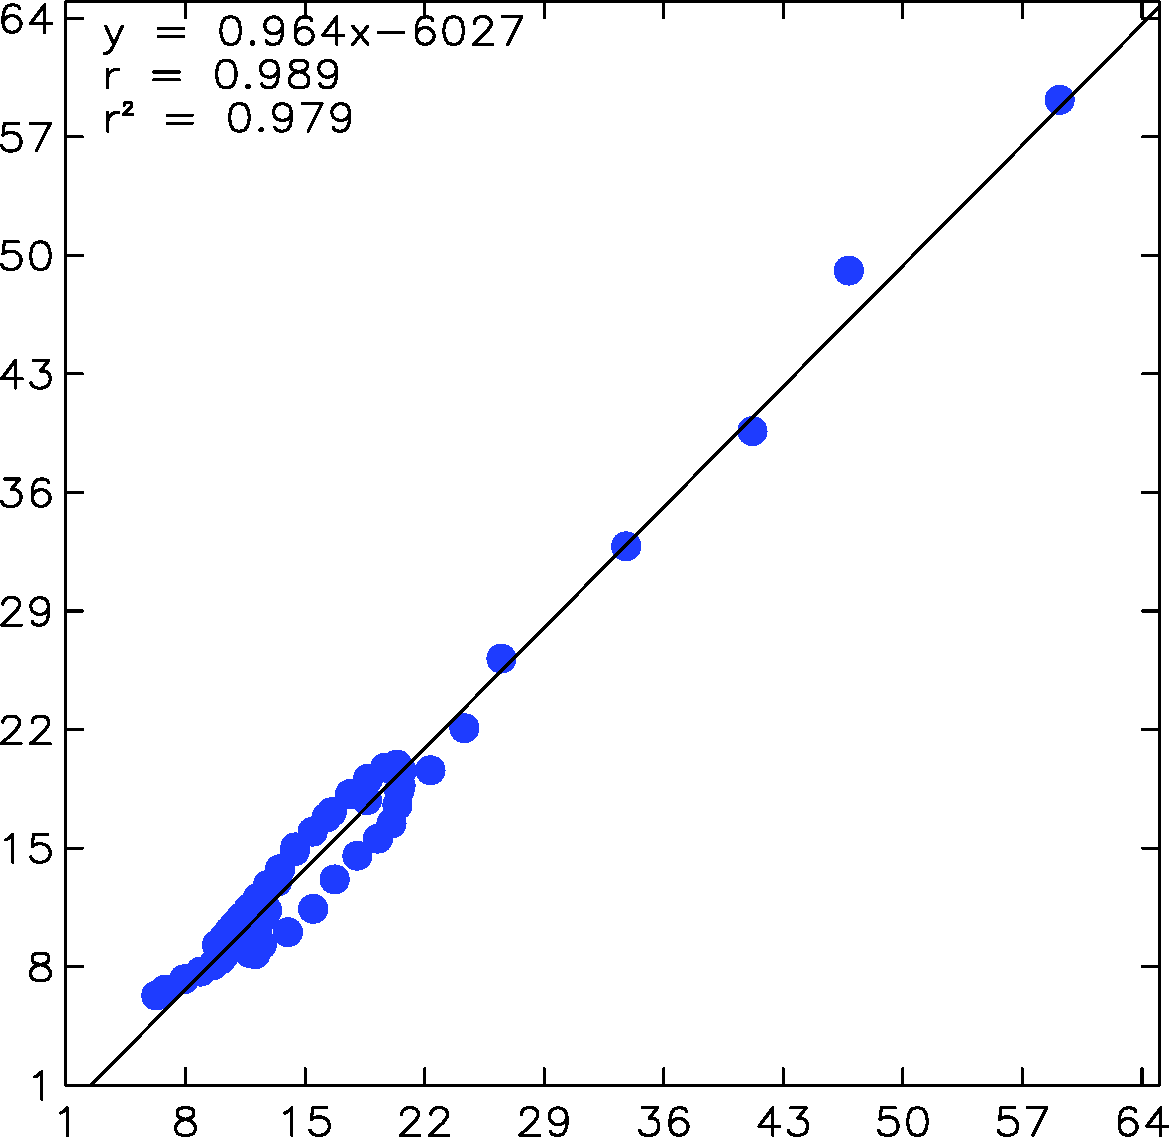
\includegraphics[width=0.3\textwidth,angle=0]{./figs/cap3/disper_novas/scatter-indiv_sf_SH_cptecAllZ_ncep-crop-rotated270.pdf}
        }\\     
        \subfigure[$\chi$ AllZ (HN)]{
            \label{fig:disper_vpAllz_hn}
            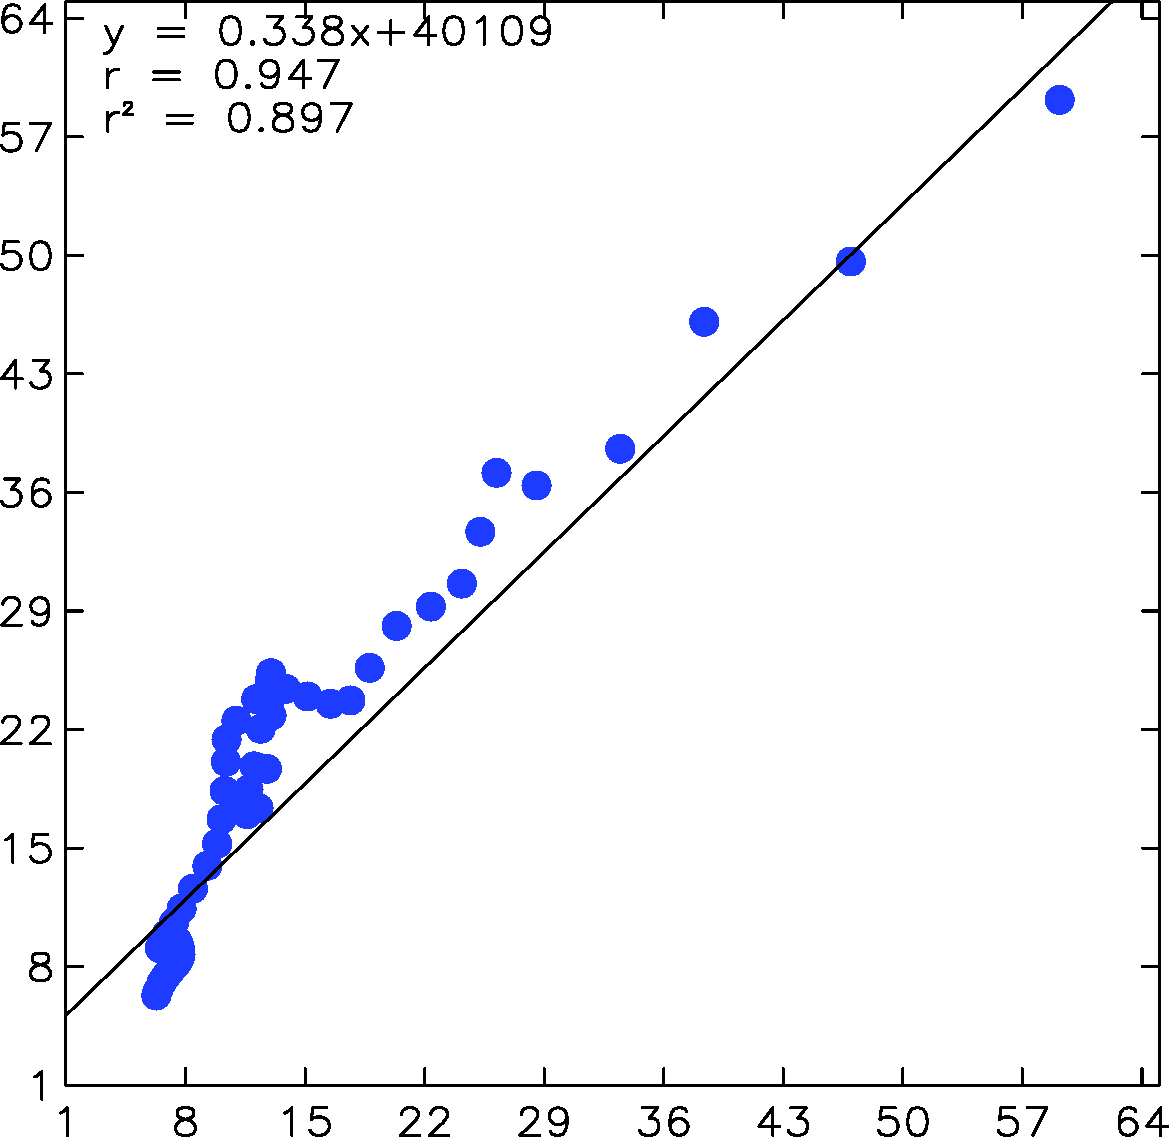
\includegraphics[width=0.3\textwidth,angle=0]{./figs/cap3/disper_novas/scatter-indiv_vp_NH_cptecAllZ_ncep-crop-rotated270.pdf}
        }
        \subfigure[$\chi$ AllZ (TR)]{
           \label{fig:disper_vpAllz_tr}
           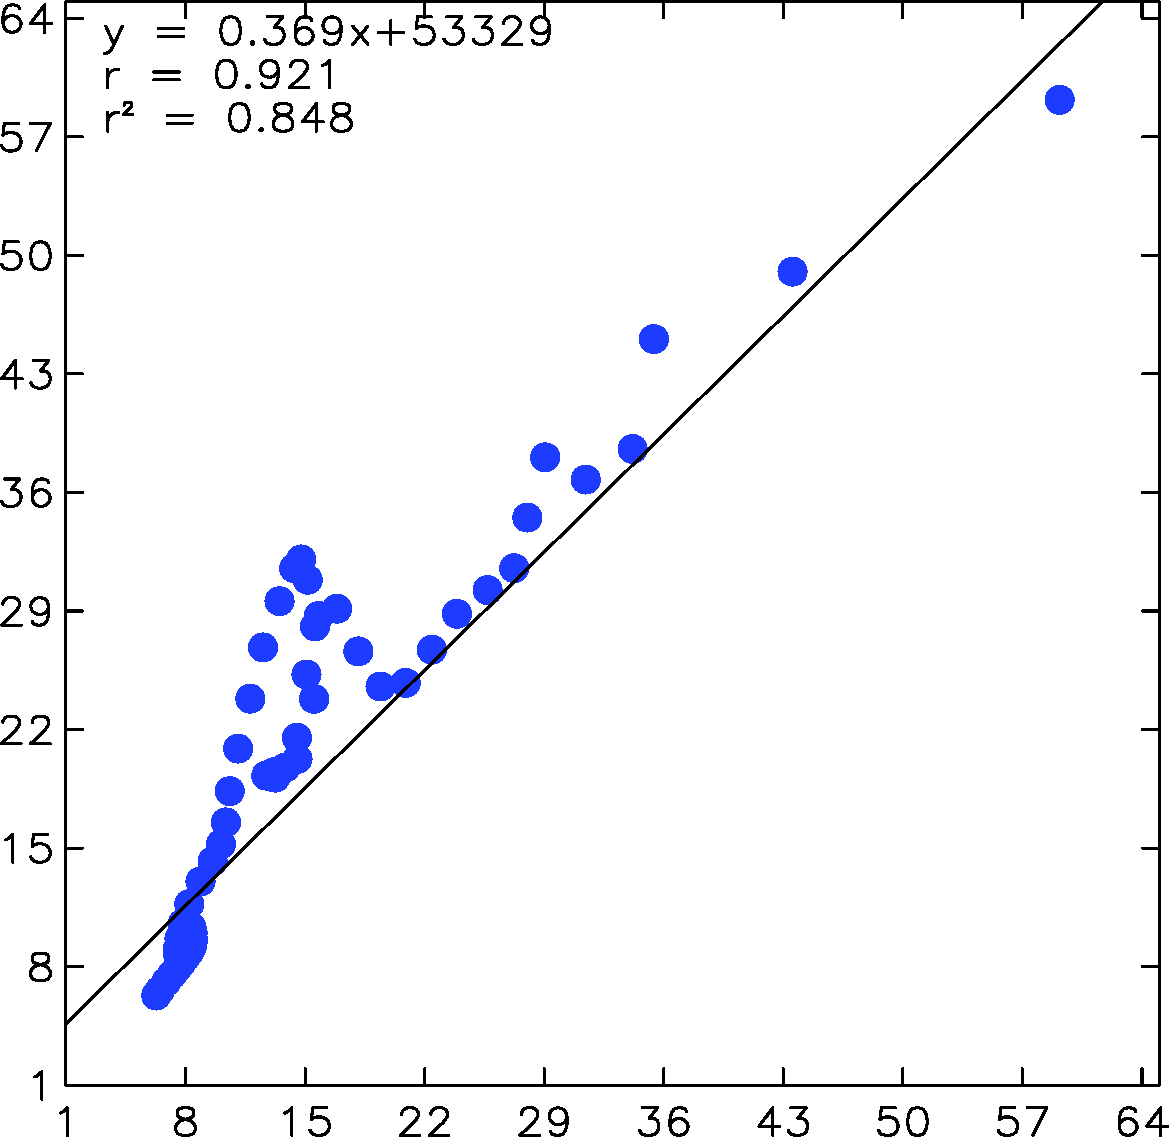
\includegraphics[width=0.3\textwidth,angle=0]{./figs/cap3/disper_novas/scatter-indiv_vp_TR_cptecAllZ_ncep-crop-rotated270.pdf}
        }
        \subfigure[$\chi$ AllZ (HS)]{
            \label{fig:disper_vpAllz_sh}
            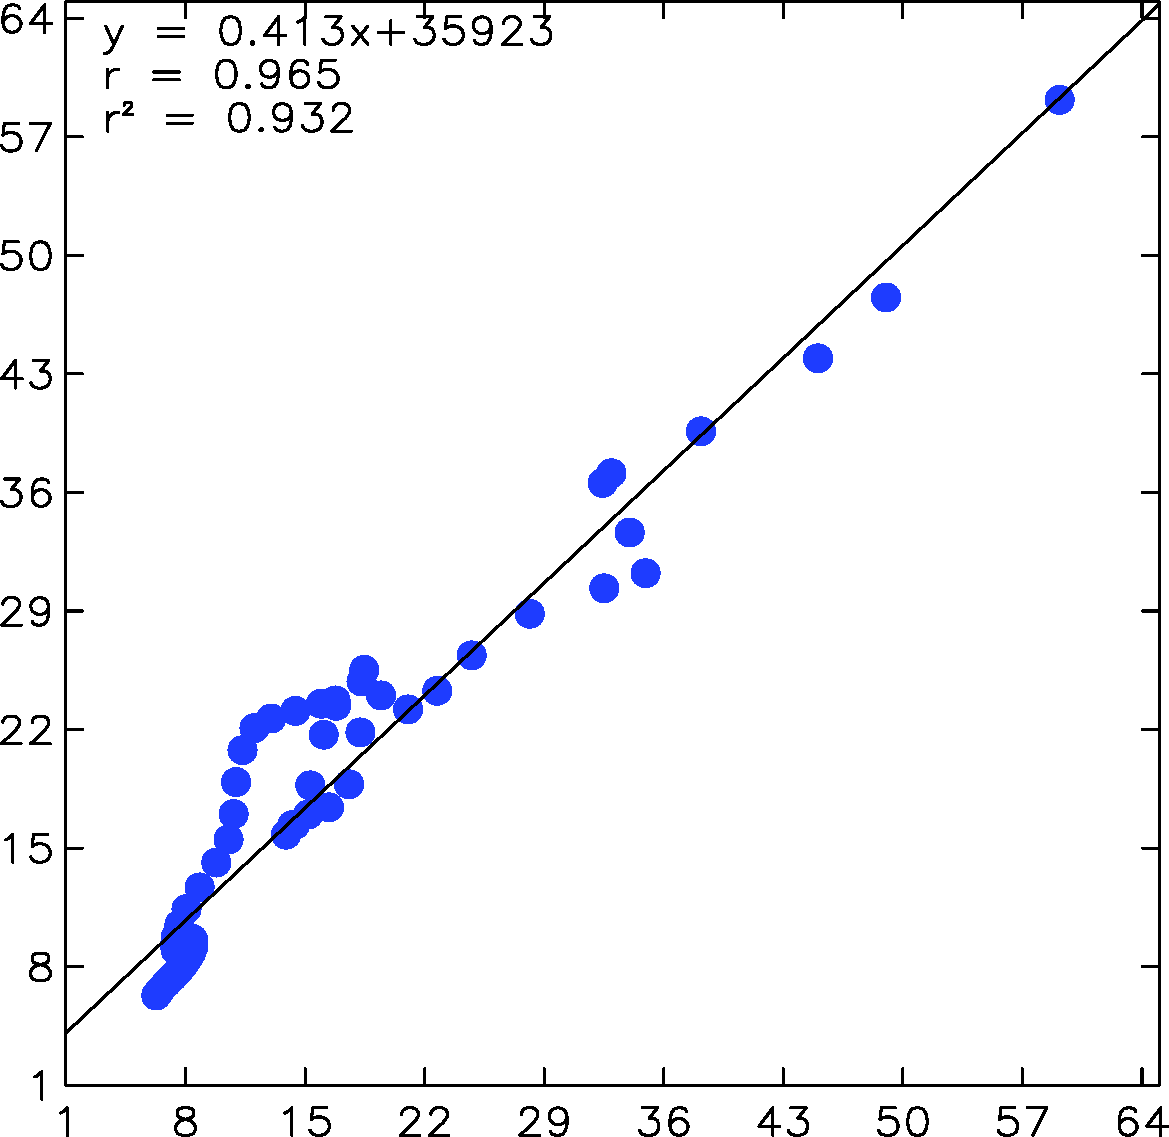
\includegraphics[width=0.3\textwidth,angle=0]{./figs/cap3/disper_novas/scatter-indiv_vp_SH_cptecAllZ_ncep-crop-rotated270.pdf}
        }\\
        \subfigure[$T$ AllZ (HN)]{
            \label{fig:disper_TAllz_hn}
            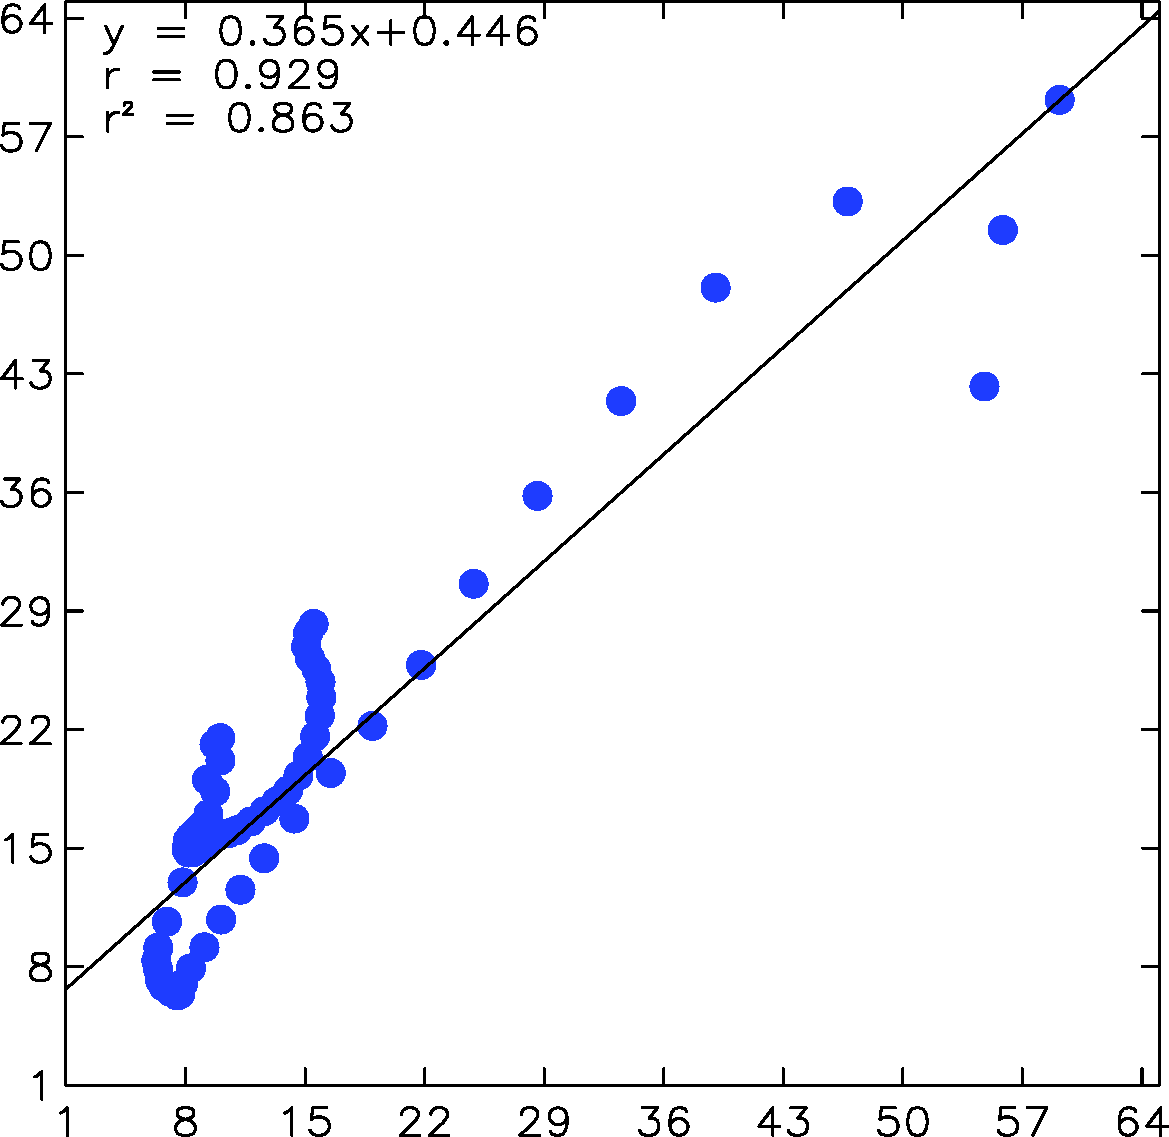
\includegraphics[width=0.3\textwidth,angle=0]{./figs/cap3/disper_novas/scatter-indiv_t_NH_cptecAllZ_ncep-crop-rotated270.pdf}
        }
        \subfigure[$T$ AllZ (TR)]{
           \label{fig:disper_TAllz_tr}
           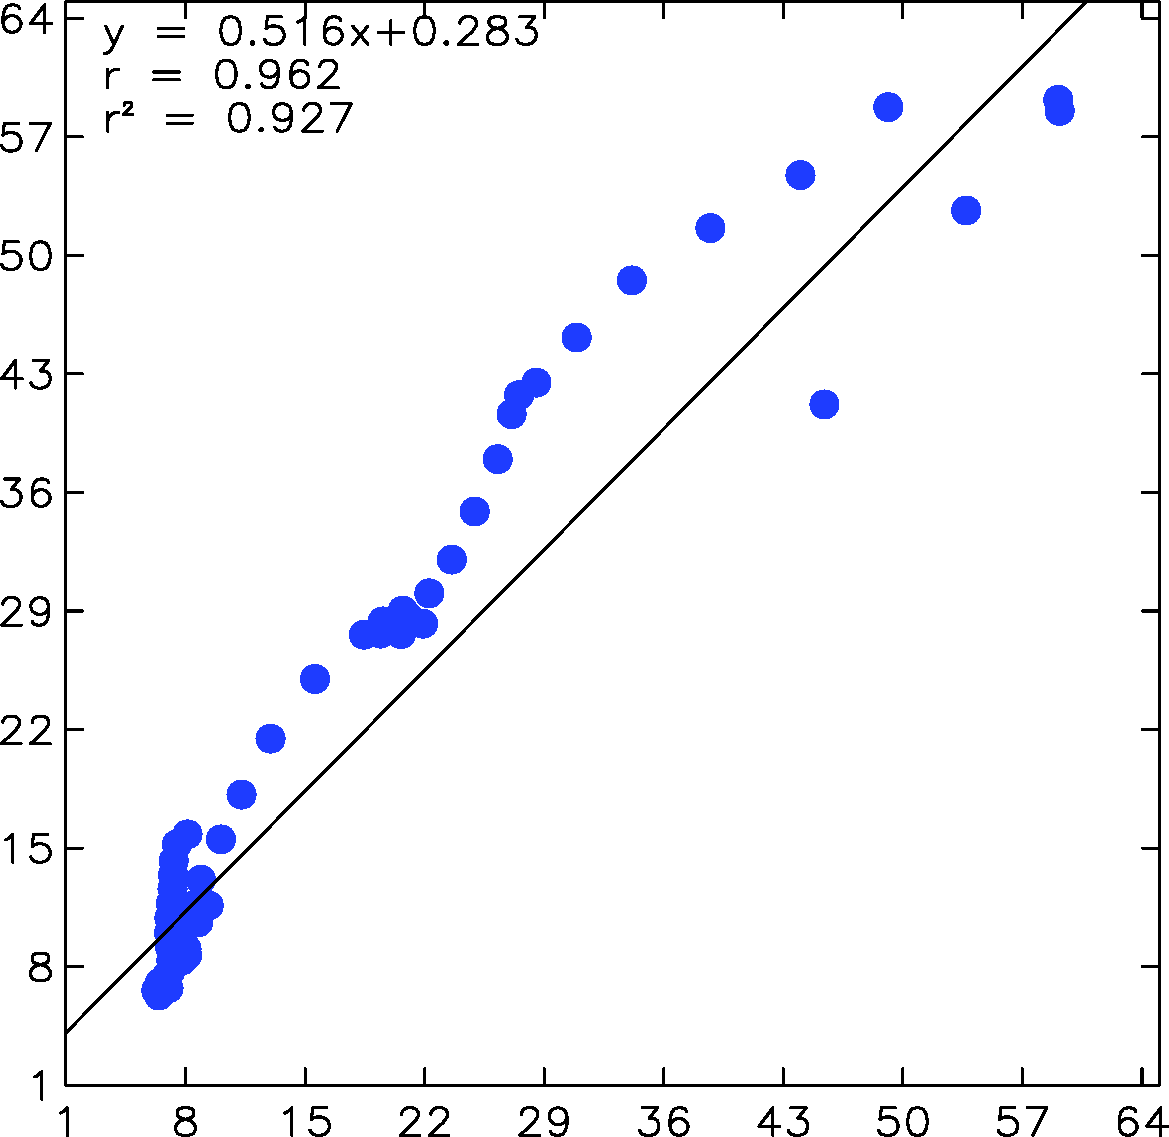
\includegraphics[width=0.3\textwidth,angle=0]{./figs/cap3/disper_novas/scatter-indiv_t_TR_cptecAllZ_ncep-crop-rotated270.pdf}
        }
        \subfigure[$T$ AllZ (HS)]{
            \label{fig:disper_TAllz_sh}
            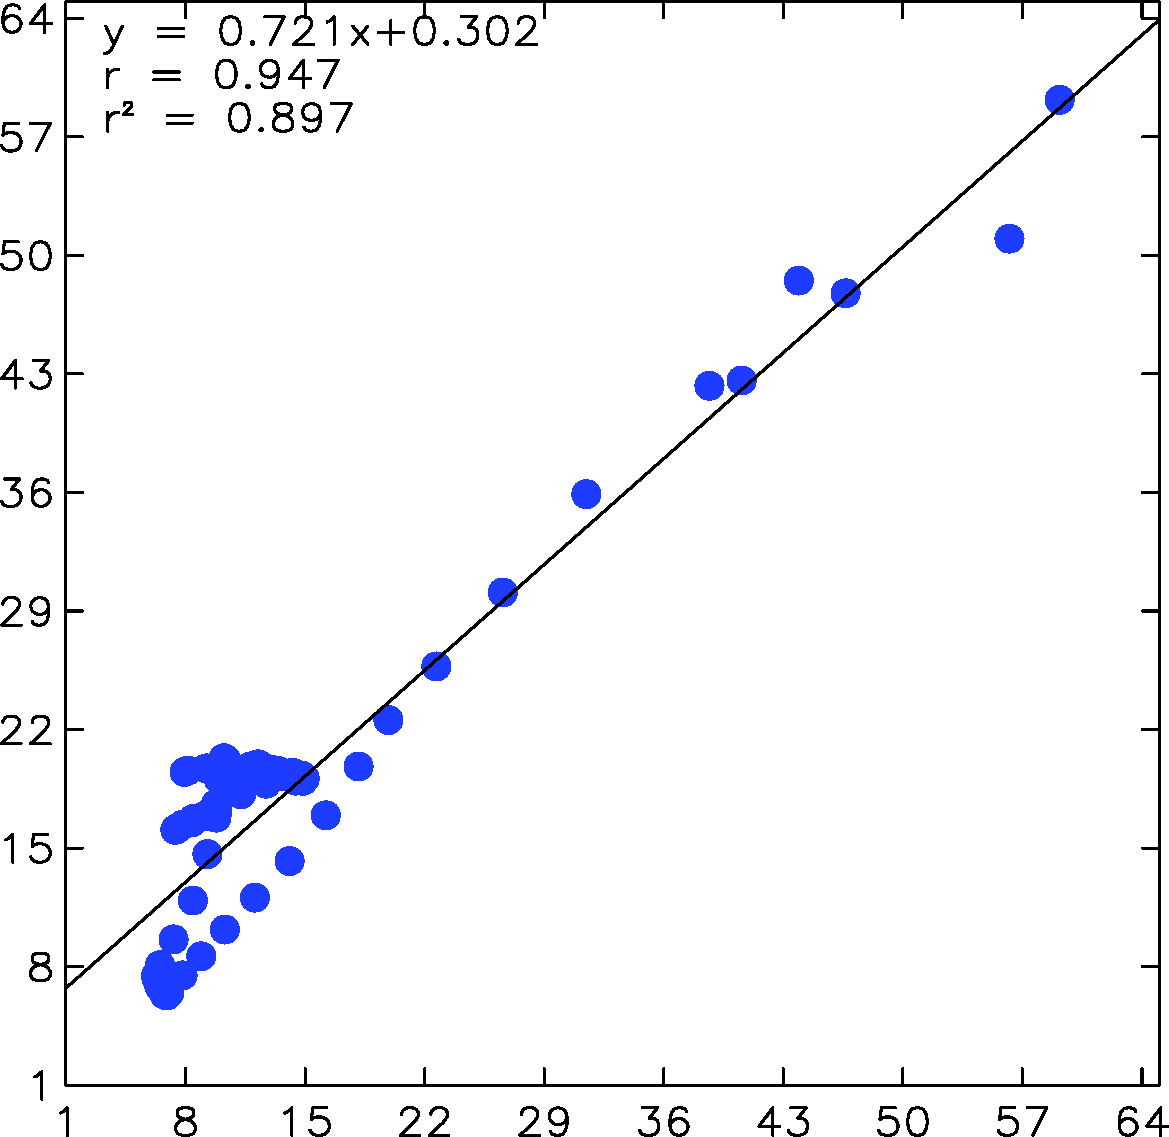
\includegraphics[width=0.3\textwidth,angle=0]{./figs/cap3/disper_novas/scatter-indiv_t_SH_cptecAllZ_ncep-crop-rotated270.pdf}
        }\\
        \subfigure[$q$ AllZ (HN)]{
            \label{fig:disper_qAllz_hn}
            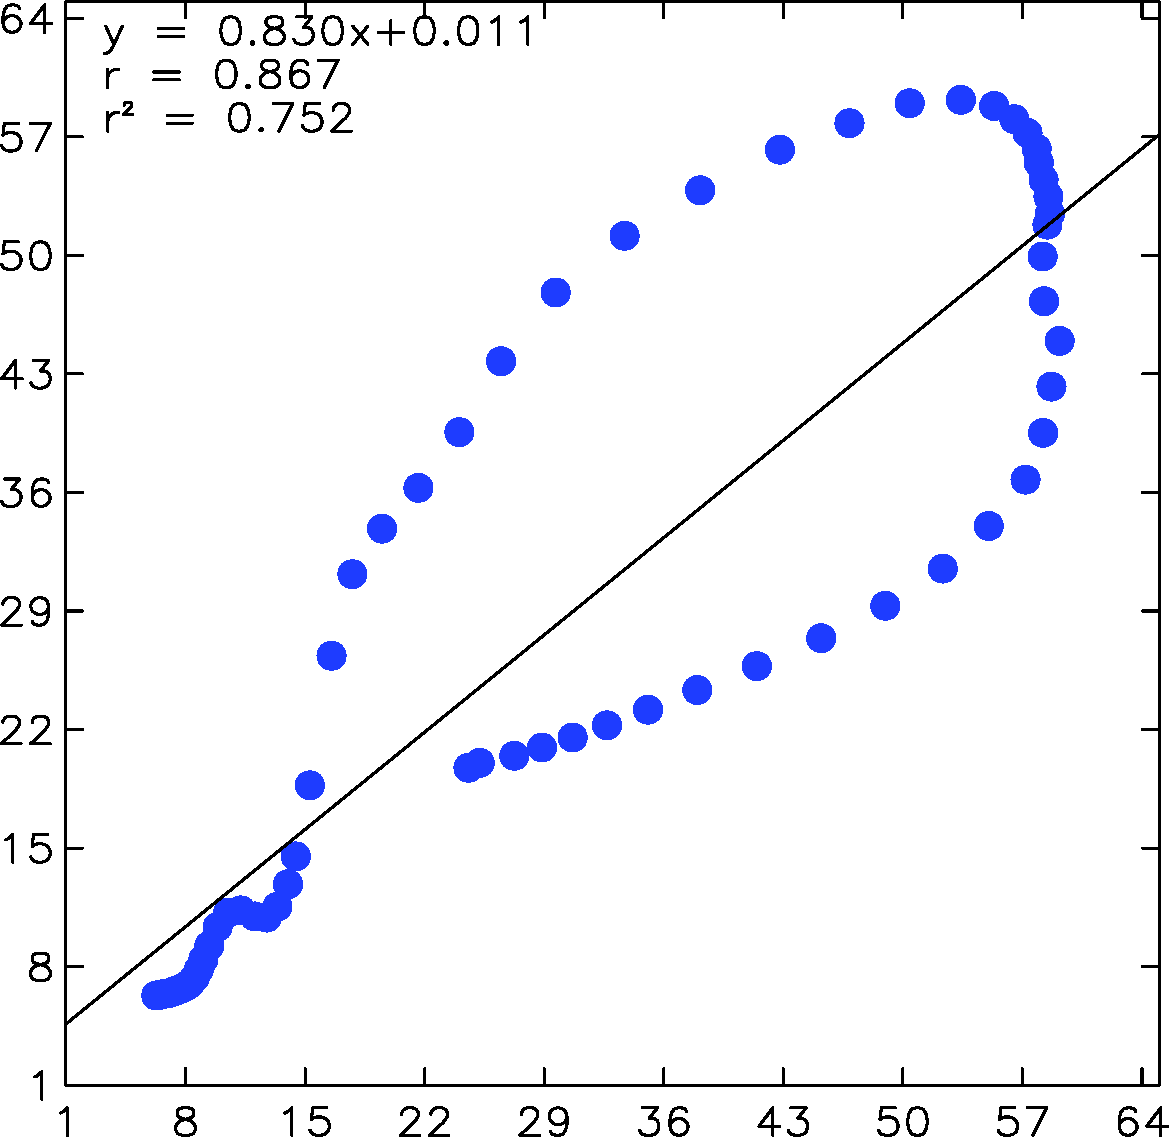
\includegraphics[width=0.3\textwidth,angle=0]{./figs/cap3/disper_novas/scatter-indiv_q_NH_cptecAllZ_ncep-crop-rotated270.pdf}
        }
        \subfigure[$q$ AllZ (TR)]{
           \label{fig:disper_qAllz_tr}
           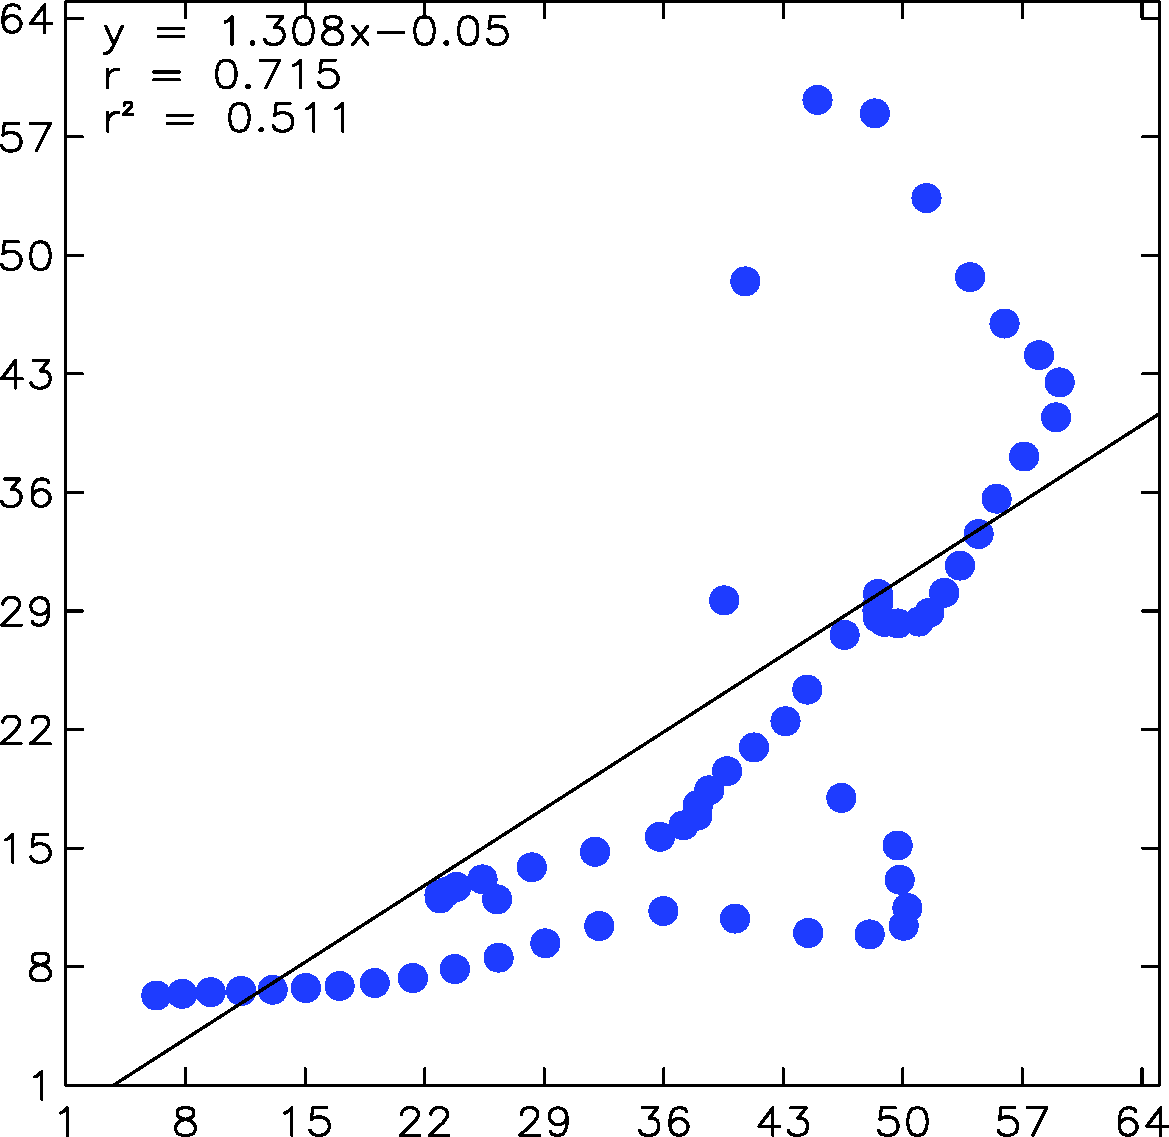
\includegraphics[width=0.3\textwidth,angle=0]{./figs/cap3/disper_novas/scatter-indiv_q_TR_cptecAllZ_ncep-crop-rotated270.pdf}
        }
        \subfigure[$q$ AllZ (HS)]{
           \label{fig:disper_qAllz_sh}
           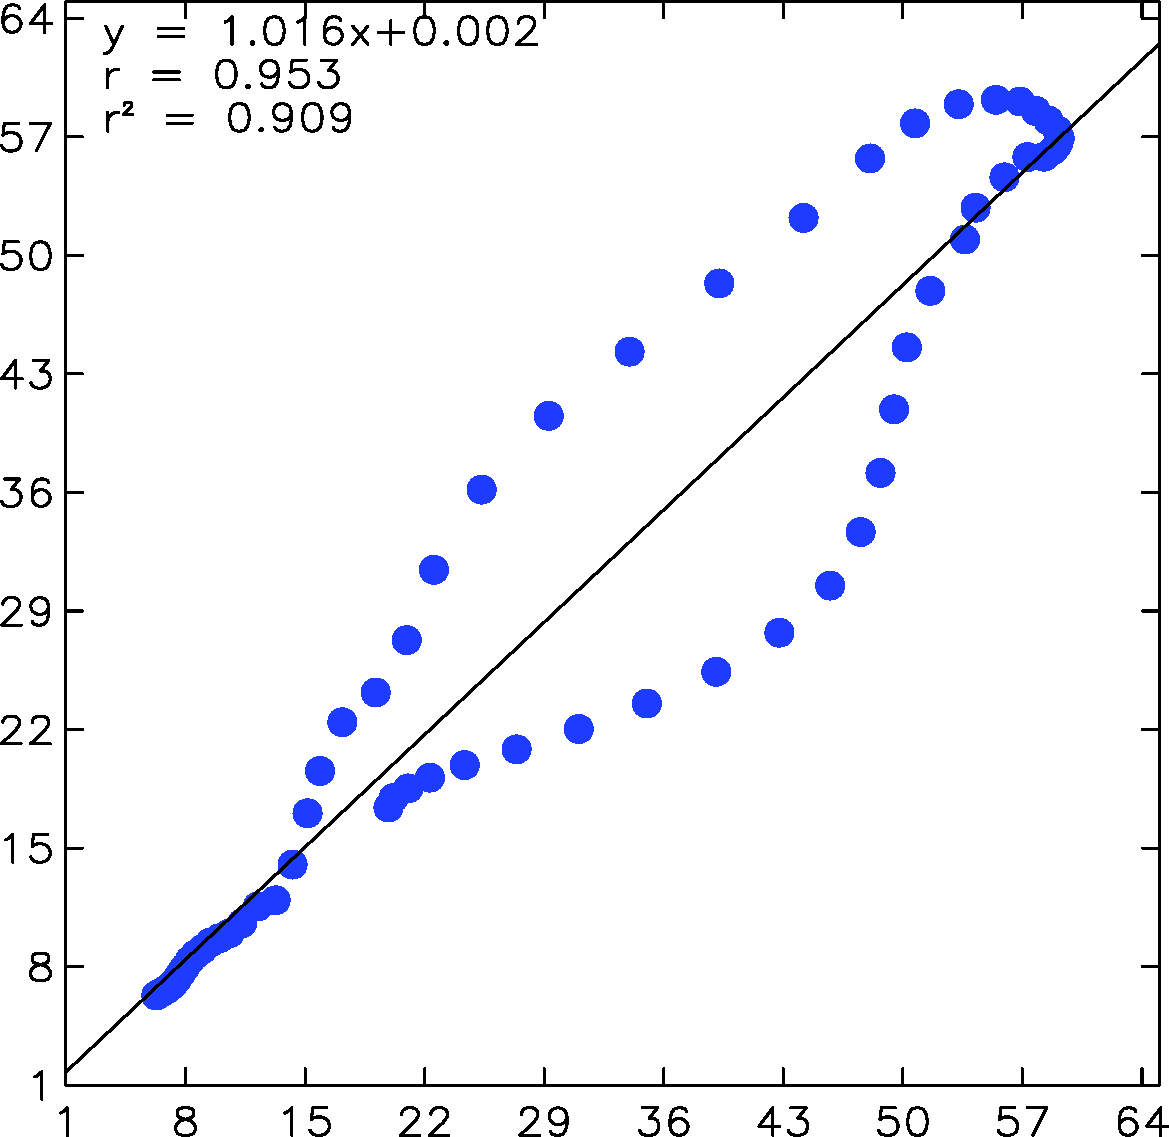
\includegraphics[width=0.3\textwidth,angle=0]{./figs/cap3/disper_novas/scatter-indiv_q_SH_cptecAllZ_ncep-crop-rotated270.pdf}
        }
  \end{center}
  \vspace{2mm}
  \legenda{Diagramas de dispersão (níveis sigma), correlações e erros quadráticos entre as amplitudes representadas nas matrizes de covariâncias $\mathbf{B}$ CPTEC e NCEP em todos os horários (AllZ), para as regiões HN (coluna a esquerda), TR (coluna do meio) e HS (coluna da direita).}
  \label{fig:disper_Allz_hn_tr_hs}
  \vspace{-4mm}
  \FONTE{Produção do autor.}
\end{figure}

\section{Aspecto do Incremento de Análise}

Como forma de verificação da influência e do impacto que a nova matriz de covariâncias do CPTEC exerce no incremento de análise do sistema G3DVAR, foi feito um experimento com a assimilação de uma única observação (sintética) no sistema. As Figuras \ref{fig:t_incr_Bcptec} e \ref{fig:t_incr_Bncep} apresentam uma comparação entre os incrementos de análise produzidos pelas matrizes de covariâncias do CPTEC e do NCEP (respectivamente).

Na Figura \ref{fig:t_incr_Bcptec}, é mostrado o incremento de análise (Previsão subtraída da Análise, ou OmA) produzido pela assimilação de uma observação sintética de vento zonal em 1000hPa. Para isto, ajustou-se o erro da observação para 1 $ms^{-1}$, bem como a magnitude da inovação trazida pela observação (Previsão subtraída da Observação, ou OmF). Neste caso, o painel da esquerda mostra o incremento de análise isotrópico (em que os pesos dados para o Filtro Recursivo nas direções $x$ e $y$ são iguais), de forma que o incremento produzido possui aspecto quase igual em todas as direções. O formato achatado no topo evidencia apenas o fato de que a observação foi posicionada mais próxima ao polo norte, mais precisamente no ponto com coordenada 0 (longitude) e 45N (latitude). No painel da direita, o incremento de análise mostrado é anisotrópico, e os parâmetros principais ajustados no GSI para a sua produção, são apresentados na Tabela \ref{tab:ajusteB}:

\begin{table}[H]
\caption{Parâmetros de configuração utilizados no sistema GSI para a aplicação das matrizes de covariâncias do CPTEC e do NCEP.}
\begin{center}
\begin{adjustbox}{max width=\textwidth}
\begin{tabular}{>{\centering\bfseries}m{2.5cm} >{\centering}m{2.5cm} >{\centering\arraybackslash}m{10cm}}
\toprule
\toprule
\multicolumn{1}{c}{\textbf{Parâmetro}} & \multicolumn{1}{c}{\textbf{Valor}} & \multicolumn{1}{c}{\textbf{Descrição}} \\
\midrule
$vs$            & 0,7             & Fator de escala do comprimento de correlação vertical \\ 
$hzscl$         & 1,7; 0,8; 0,5   & Fator de suavização para as 3 escalas horizontais \\ 
$hswgt$         & 0,45; 0,3; 0,25 & Pesos aplicados a cada escala horizontal \\ 
$bw$            & 0               & Fator no cálculo da covariância do erro \\ 
$norsp$         & 4               & Ordem de suavização horizontal das covariâncias do erro de previsão \\ 
$bkg\_flowdep$  & True/False      & Flag para usar (True = anisotrópico) ou não (False = isotrópico) a dependência das variâncias do erro de previsão \\
\bottomrule
\end{tabular}
\end{adjustbox}
\end{center}
\label{tab:ajusteB}
\end{table}

O parâmetro ``$vs$'', ajusta a escala vertical e sua unidade é dada em pontos de grade; o parâmetro ``$hzscl$'', ajusta a escala horizontal e o parâmetro ``$hswgt$'' ajusta os pesos dados a aplicação do filtro recursivo nas direções $x$, $y$ e $z$, respectivamente.

\begin{figure}[H]
    \vspace{2mm}
    \caption{Aspectos dos incrementos de análise utilizando a nova matriz de covariâncias do CPTEC.}
    \begin{center}
        \subfigure[$\mathbf{B}$ CPTEC lat x lon (Isotrópica)]{
            \label{fig:t_incr_Bcptec_lat_lon_iso}
            \includegraphics[width=0.47\textwidth]{./figs/cap3/incrementos_novas/incr_bcptec_iso_lat_lon-crop-rotated270.pdf}
        }     
        \subfigure[$\mathbf{B}$ CPTEC lat x lon (Anisotrópica)]{
            \label{fig:t_incr_Bcptec_lat_lon_aniso}
            \includegraphics[width=0.47\textwidth]{./figs/cap3/incrementos_novas/incr_bcptec_aniso_lat_lon-crop-rotated270.pdf}
        }\\
        \subfigure[$\mathbf{B}$ CPTEC lat x lev (Isotrópica)]{
            \label{fig:t_incr_Bcptec_lat_lev_iso}
            \includegraphics[width=0.47\textwidth]{./figs/cap3/incrementos_novas/incr_bcptec_iso_lat_lev-crop-rotated270.pdf}
        }
        \subfigure[$\mathbf{B}$ CPTEC lat x lev (Anisotrópica)]{
           \label{fig:t_incr_Bcptec_lat_lev_aniso}
           \includegraphics[width=0.47\textwidth]{./figs/cap3/incrementos_novas/incr_bcptec_aniso_lat_lev-crop-rotated270.pdf}
        }\\
        \subfigure[$\mathbf{B}$ CPTEC lon x lev (Isotrópica)]{
            \label{fig:t_incr_Bcptec_lon_lev_iso}
            \includegraphics[width=0.47\textwidth]{./figs/cap3/incrementos_novas/incr_bcptec_iso_lon_lev-crop-rotated270.pdf}
        }
        \subfigure[$\mathbf{B}$ CPTEC lon x lev (Anisotrópica)]{
           \label{fig:t_incr_Bcptec_lon_lev_aniso}
           \includegraphics[width=0.47\textwidth]{./figs/cap3/incrementos_novas/incr_bcptec_aniso_lon_lev-crop-rotated270.pdf}
        }\\
        \includegraphics[width=0.75\textwidth]{./figs/cap3/incrementos_novas/cbar-crop-rotated270.pdf}
    \end{center}
    \vspace{2mm}
    \legenda{Incremento de análise da temperatura ($T$) ano nível de 1000 hPa, utilizando a nova matriz de covariâncias do CPTEC: a esquerda, incremento isotrópico; a direita incremento anisotrópico.}
   \label{fig:t_incr_Bcptec}
   \FONTE{Produção do autor.}
\end{figure}
    
A Figura \ref{fig:t_incr_Bncep} apresenta o incremento de análise produzido pela matriz de covariâncias do NCEP, aplicada ao sistema G3DVAR, assimilando a mesma observação sintética única, no mesmo nível e com as mesmas magnitudes de erro e inovação. De forma geral, para ambos os casos (isotrópico e anisotrópico), o incremento de análise calculado pela matriz de covariâncias do CPTEC (matriz CPTEC BAllZ), produz um incremento mais largo, abrangendo mais pontos de grade em todas as direções. Isso significa que o incremento de análise calculado, é espalhado sobre uma região maior ao redor da vizinhança da observação e que a sua influência pode ser transportada para mais longe. Em uma situação física em que, por exemplo há a incursão de um sistema frontal e, considerando-se o caso anisotrópico, a assimilação de dados pode trazer um benefício importante para a previsão gerada, porque a análise utilizada possuirá um balanço melhor entre observações e previsão. Isso mostra a importância da seleção das observações, do controle de qualidade e do \textit{thinning} do sistema (i.e., o controle espacial das observações). Além disso, a magnitude do incremento de análise produzido pela matriz de covariâncias do CPTEC é mais suave, embora seja menos concentrado. Em contraste, a matriz de covariâncias do NCEP, apresenta incrementos muito mais concentrados e um pouco mais intensos também.    
    
\begin{figure}[H]
    \vspace{2mm}
    \caption{Idem Figura \ref{fig:t_incr_Bcptec}, para a matriz de covariâncias do NCEP.}
    \begin{center}
        \subfigure[$\mathbf{B}$ NCEP lat x lon (Isotrópica)]{
            \label{fig:t_incr_Bncep_lat_lon_iso}
            \includegraphics[width=0.47\textwidth]{./figs/cap3/incrementos_novas/incr_bncep_iso_lat_lon-crop-rotated270.pdf}
        }     
        \subfigure[$\mathbf{B}$ NCEP lat x lon (Anisotrópica)]{
            \label{fig:t_incr_Bncep_lat_lon_aniso}
            \includegraphics[width=0.47\textwidth]{./figs/cap3/incrementos_novas/incr_bncep_aniso_lat_lon-crop-rotated270.pdf}
        }\\
        \subfigure[$\mathbf{B}$ NCEP lat x lev (Isotrópica)]{
            \label{fig:t_incr_Bncep_lat_lev_iso}
            \includegraphics[width=0.47\textwidth]{./figs/cap3/incrementos_novas/incr_bncep_iso_lat_lev-crop-rotated270.pdf}
        }
        \subfigure[$\mathbf{B}$ NCEP lat x lev (Anisotrópica)]{
           \label{fig:t_incr_Bncep_lat_lev_aniso}
           \includegraphics[width=0.47\textwidth]{./figs/cap3/incrementos_novas/incr_bncep_aniso_lat_lev-crop-rotated270.pdf}
        }\\
        \subfigure[$\mathbf{B}$ NCEP lon x lev (Isotrópica)]{
            \label{fig:t_incr_Bncep_lon_lev_iso}
            \includegraphics[width=0.47\textwidth]{./figs/cap3/incrementos_novas/incr_bncep_iso_lon_lev-crop-rotated270.pdf}
        }
        \subfigure[$\mathbf{B}$ NCEP lon x lev (Anisotrópica)]{
           \label{fig:t_incr_Bncep_lon_lev_aniso}
           \includegraphics[width=0.47\textwidth]{./figs/cap3/incrementos_novas/incr_bncep_aniso_lon_lev-crop-rotated270.pdf}
        }\\
        \includegraphics[width=0.75\textwidth]{./figs/cap3/incrementos_novas/cbar-crop-rotated270.pdf}
    \end{center}
    \vspace{2mm}
    \legenda{Incremento de análise da temperatura ($T$) ano nível de 1000 hPa, utilizando a matriz de covariâncias do NCEP: a esquerda, incremento isotrópico; a direita incremento anisotrópico.}
   \label{fig:t_incr_Bncep}
   \FONTE{Produção do autor.}
\end{figure}
\chapter{ASSIMILAÇÃO DE DADOS HÍBRIDA ENSEMBLE-VARIACIONAL GLOBAL}
\label{cap:incorpora_covars}

Neste capítulo é apresentada a metodologia para a incorporação das covariâncias do filtro de Kalman por conjunto (Seções \ref{sec:enkf} e \ref{sec:ensrf}) na estrutura variacional do sistema GSI (Seção \ref{sec:3dvar}). O código computacional dos sistemas EnKF e EnSRF já havia sido previamente programado e estava sendo testado pelo GMAO em suas aplicações de pesquisa no sistema híbrido proposto por eles. Para o caso do sistema híbrido 3DVar do CPTEC em uso com o modelo de circulação geral do centro, não foram necessárias modificações no código computacional, com excessão do tratamento do ozônio sendo este ajustado para ser univariado (i.e., não é considerada a sua covariância com as demais variáveis da matriz de covariâncias). Isso foi necessário devido aos problemas iniciais que foram encontrados com a representação do ozônio na matriz de covariâncias calculada para o MCGAv4.

Na seção a seguir é apresentada a metodologia de incorporação das covariâncias do filtro de Kalman por conjunto na estrutura variacional. Esta metodologia segue as ideias introduzidas por \citeonline{lorenc/2003} e aplicadas por \citeonline{wangetal/2008a,wangetal/2008b,wang/2010} no sistema GSI. A notação das equações foi alterada para ficar em conformidade com os demais desenvolvimentos apresentados no trabalho. Além da apresentação da metodologia para a incorporação das covariâncias, são apresentadas também as configurações utilizadas no sistema para que fosse possível realizar o ciclo de análises e previsões de forma satisfatória, o que inclui a determinação de parâmetros fundamentais para a assimilação de dados como a configuração das iterações da minimização da função custo, o controle da umidade não física, porcentagem de contribuição das covariâncias do conjunto entre outros. É apresentado também um diagrama esquemático ilustrando o ciclo de assimilação de dados do sistema híbrido. Neste diagrama são apresentadas também as principais equações envolvidas nas diferentes etapas do processo. Ao final do capítulo, é apresentado como é feita a análise do campo de vento horizontal no GSI, uma vez que diferentes quantidades para representar o vento estão envolvidas no processo de assimilação de dados e previsão.

\section{Incorporação das Covariâncias do filtro de Kalman por conjunto na Estrutura Variacional do GSI}

A técnica utilizada para incorporar as covariâncias dos erros de previsão provenientes do filtro de Kalman por conjunto (EnKF/EnSRF) na estrutura variacional tridimensional (3DVar) do GSI, é aquela apresentada por \citeonline{lorenc/2003} denominada ``Variável de Controle Alpha'' e também em \citeonline{wangetal/2008a,wangetal/2008b,wang/2010} denominada ``Variável de Controle Estendida''. A técnica de incorporação ou inclusão das covariâncias dos erros de previsão na estrutura variacional consiste na definição de um novo incremento de análise ($\delta{\mathbf{x}}'$) e de uma matriz de correlações ($\mathbf{C}$), cujos elementos são multiplicados pelos elementos da matriz de covariâncias dos erros de previsão proveniente do filtro de Kalman por conjunto ($\mathbf{P}^{b}$). Esta abordagem é semelhante aquela empregada nos trabalhos de \citeonline{claytonetal/2012} e \citeonline{wangelei/2013}. 

No sistema híbrido, o novo incremento de análise denotado por $\delta{\mathbf{x}}'$ é a soma de dois termos, definida como:

\begin{equation}
\label{eq:29}
\delta{\mathbf{x}'} = \delta{\mathbf{x}} + \sum_{k=1}^{K}{(\mathbf{x}_{k}^{e} \circ \mathbf{a}_{k})}
\end{equation}

onde:

\begin{itemize}
    \item $\delta{\mathbf{x}'}$: é o novo incremento de análise híbrido (dimensão: $n$ x $1$);
    \item $\delta{\mathbf{x}}$: é o incremento de análise original (i.e., $\mathbf{x}^{a}-\mathbf{x}^{b}$; $n$ x $1$);
    \item $\mathbf{a}_{k}$: é a extensão da variável de controle a ser analisada para cada membro do conjunto de $K$ previsões ($n$ x $k$);
    \item $\mathbf{x}_{k}^{e}$: é a $k$-ésima previsão do conjunto ($n$ x $1$).
\end{itemize}

Na Eq. \ref{eq:29}, o primeiro termo do lado direito da equação ($\delta{\mathbf{x}}$), é o incremento de análise associado com a covariância estática do erro de previsão ($\mathbf{B}$). O segundo termo ($\sum_{k=1}^{K}{\mathbf{x}_{k}^{e} \circ \mathbf{a}_{k}}$), é o incremento associado as covariâncias ($\mathbf{P}^{b}$) provenientes do filtro de Kalman por conjunto. Os vetores $\mathbf{a}_{k}$ (com $k=1,...,K$), denotam as extensões das variáveis de controle para cada membro (os quais serão explicados com mais detalhes adiante). O símbolo $\circ$ representa o produto Schur (i.e., elemento a elemento) entre os elementos dos vetores $\mathbf{a}_{k}$ e $\mathbf{x}_{k}^{e}$. Em outras palavras, o segundo termo na Eq. \ref{eq:29}, representa a combinação linear local das perturbações do conjunto com o incremento de análise original ($\delta{\mathbf{x}}$). O coeficiente $\mathbf{a}_{k}$ para cada membro varia espacialmente, o qual determina a escala espacial de localização horizontal do conjunto. Ainda na Eq. \ref{eq:29}, o vetor $\mathbf{x}_{k}^{e}$ representa a $k$-ésima perturbação do conjunto normalizada por $\sqrt{K-1}$, onde $K$ é o tamanho do conjunto de previsões. Este vetor é determinado pela Eq. \ref{eq:30}:

\begin{equation}
\label{eq:30}
\mathbf{x}_{k}^{e} = \frac{(\mathbf{x}_{k}^{b} - \bar{\mathbf{x}}^{b})}{\sqrt{K-1}}
\end{equation}

onde:

\begin{itemize}
    \item $\mathbf{x}_{k}^{e}$: é a $k$-ésima perturbação do conjunto de $K$ membros de previsão (dimensão: $n$ x $k$);
    \item $\mathbf{x}_{k}^{b}$: é o $k$-ésimo membro do conjunto de previsões ($n$ x $1$);
    \item $\bar{\mathbf{x}}^{b}$: é a média do conjunto de $K$ previsões ($n$ x $1$).
\end{itemize}

No sistema híbrido 3DVar, a solução da análise segue a abordagem variacional do 3DVar, com a análise sendo calculada a partir da minimização da função-custo (um passo a passo da minimização da função custo variacional tridimensional é apresentada no Apêndice \ref{apendiceI}, entre as Eqs. \ref{apI_eq:1} e \ref{apI_eq:22}). Com o novo incremento de análise definido para o híbrido, a função custo representada pela Eq. \ref{eq:fcusto} (na forma incremental na Eq. \ref{eq:31}) pode ser reescrita considerando-se uma combinação linear entre o termo da função custo referente ao incremento de análise variacional do 3DVar denotada por $\textit{J}_{3dvar,1}$ e o termo referente a extensão da variável de controle $a$ denotada por $\textit{J}_{e}$, que é proveniente do Filtro de Kalman por ensemble, além do termo referente as inovações denotado aqui por $\textit{J}_{3dvar,2}$: 

\begin{equation}
\label{eq:31}
\textit{J}_{3dvar}(\delta\mathbf{x}) = \underbrace{\frac{1}{2} (\delta\mathbf{x})^{T}\mathbf{B}^{-1}(\delta\mathbf{x})}_{\text{\textit{J}\_{3dvar,1}}} + \underbrace{\frac{1}{2} [\mathbf{y}^{o} - \textit{H}(\mathbf{x}^{b})]^{T}\mathbf{R}^{-1}[\mathbf{y}^{o} - \textit{H}(\mathbf{x}^{b})] }_{\text{\textit{J}\_{3dvar,2}}}
\end{equation}

A Eq. \ref{eq:32} abaixo, representa a base sobre a qual o sistema híbrido ensemble-variacional é fundamentado:

\begin{equation}
\label{eq:32}
J(\delta\mathbf{x},\mathbf{a}) = \alpha_{1} J_{3dvar,1} + \alpha_{2} J_{e} + J_{3dvar,2}
\end{equation}

onde:

\begin{itemize}
\item $J_{3dvar,1}$: é o termo da função custo variacional do 3DVar referente ao incremento de análise original;
\item $J_{3dvar,2}$: é o termo da função custo variacional do 3DVar referente a inovação original;
%\item $J_{e}$: é o novo termo adicionado a função custo, referente à matriz de correlação espacial horizontal $\mathbf{A}$;
\item $J_{e}$: é o novo termo adicionada a função custo variacional, referente a aplicação da extensão da variável de controle (indicado na Eq. \ref{eq:33} a seguir);
\item $\delta\mathbf{x}$: é o incremento de análise devido a contribuição da matriz de covariâncias estática;
\item $\alpha_{1}$ e $\alpha_{2}$: são os pesos empíricos atribuídos as contribuições das matrizes de covariâncias estática e fluxo-dependente, respectivamente ($\alpha_{n} \in [0,1]$, $n=1,2$).
%\item ${y'}^{o}$: é o vetor inovação, sendo ${y'}^{o}=y^{o}-H(x^{b})$ em que $y^{o}$ é o vetor observação, $H$ é o operador observação não linear e $x^{b}$ o vetor background (que no sistema híbrido é a média do ensemble de background).
\end{itemize}

\citeonline{wangetal/2008a,wangetal/2008b} utilizam da igualdade ${\mathbf{y}}^{\prime{o}} = \mathbf{y}^{o} - \textit{H}(\mathbf{x}^{b})$ para escrever a forma incremental da função custo híbrida em termos da extensão da variável de controle (Eq. \ref{eq:33}), e em sua forma final, Eq. \ref{eq:34}:

\begin{equation}
\label{eq:33}
\begin{aligned}
J(\delta{\mathbf{x}'},\mathbf{a}) = {} & \alpha_{1} \frac{1}{2} (\delta{\mathbf{x}'})^{T}\mathbf{B}^{-1}(\delta{\mathbf{x}'}) + \alpha_{2} \frac{1}{2} (\mathbf{a})^{T}\mathbf{A}^{-1}(\mathbf{a}) \\
& + \frac{1}{2} [{\mathbf{y}}^{\prime{o}} - \mathbf{H}(\delta{\mathbf{x}})]^{T}\mathbf{R}^{-1}[{\mathbf{y}}^{\prime{o}} - \mathbf{H}(\delta{\mathbf{x}})]
\end{aligned}
\end{equation}

\begin{equation}
\label{eq:34}
J(\delta{\mathbf{x}'}) = \frac{1}{2} (\delta{\mathbf{x}'})^{T} (\alpha_{1}\mathbf{B}+\alpha_{2}\mathbf{P}^{b}\circ\mathbf{A})^{-1} (\delta{\mathbf{x}'}) + \frac{1}{2} [{\mathbf{y}}^{\prime{o}} - \mathbf{H}(\delta{\mathbf{x}'})]^{T}\mathbf{R}^{-1}[{\mathbf{y}}^{\prime{o}} - \mathbf{H}(\delta{\mathbf{x}'})]
\end{equation}

onde:

\begin{itemize}
    \item $\mathbf{P}^{b}$: é a matriz de covariâncias dos erros do conjunto de previsões, tal como definida nas Eqs. \ref{eq:enkf_pb} e \ref{eq:enkf_pbe1};
    \item $\mathbf{A}$: é uma matriz de correlação que faz a localização horizontal das covariâncias dos erros do conjunto. Ela é formada pelos vetores $\mathbf{a}_{k}$ e, tal como a matriz $\mathbf{B}$, sua aplicação se dá através de um filtro recursivo, como o que está apresentado no Apêndice \ref{apendiceV}.
\end{itemize}

Para conservar a variância do erro da previsão na Eq. \ref{eq:34}, os parâmetros $\alpha_{1}, \alpha_{2}$ são restringidos pela relação $\alpha_{1} + \alpha_{2} = 1$. Logo uma contribuição de, eg., 75\% das covariâncias do conjunto de previsões (i.e., através de $\mathbf{P}^{b}$) implica em $\alpha_{2}=0,75$ e consequentemente $\alpha_{1}=0,25$.

\section{Ajustes dos Parâmetros Principais}

Nesta seção são apresentados os aspectos principais relacionados com as diversas componentes que compõem o sistema híbrido 3DVar. Algumas destas componentes devem ser configuradas e outras estabelecidas para a realização cíclica do sistema híbrido. Em alguns casos, as opções padrão foram adotadas e em outras, soluções a parte tiveram que ser criadas. % como é o caso das tabelas lidas pelo radinfo do gsi e enkf.

\subsection{Matriz de Covariâncias Estática (B)}

Nesta subseção, são apresentadas as principais componentes e opções relacionadas com a determinação e aplicação da matriz de covariâncias estática dos erros de previsão.

\subsubsection*{Aplicação das Covariâncias Estáticas}

Diferentemente da matriz idealizada apresentada na Figura \ref{fig:1}, a matriz de covariâncias do GSI contém as seguintes estruturas: amplitudes (representadas pelos desvios-padrão e variâncias), distâncias (representadas pelos comprimentos de escalas horizontais e verticais) e matrizes de projeção de balanço (representadas por coeficientes de regressão). Nesta versão da matriz de covariâncias utilizada pelo GSI (independente da versão do modelo de circulação geral do CPTEC) as amplitudes são representadas por médias zonais (as quais podem ser ponderadas durante o processo de minimização da função custo), variando apenas nas latitudes e na vertical. As partes desbalanceadas das variáveis velocidade potencial ($\chi$), temperatura virtual ($T$) e pressão em superfície ($ps$), possuem matrizes de projeção ($\mathbf{G}$ e $\mathbf{W}$, nas Eqs. \ref{eq:tempbal} e \ref{eq:presbal} respectivamente) que são responsáveis por projetar o incremento de análise da função de corrente ($\psi$) no perfil vertical da parte balanceada do incremento de cada uma destas variáveis. Para a velocidade potencial, uma matriz de correlação ($\mathbf{C}$ na Eq. \ref{eq:velbal}) é utilizada para contabilizar a correlação positiva entre divergência ($D$) e vorticidade ($\zeta$). 

\begin{align}
\label{eq:tempbal}
    T_{b}=\mathbf{G}\psi \\
\label{eq:presbal}
    P_{b}=\mathbf{W}\psi \\
\label{eq:velbal}
    \chi_{b}=\mathbf{C}\psi
\end{align}

onde, nas Eqs. \ref{eq:tempbal}, \ref{eq:presbal} e \ref{eq:velbal} o subscrito $b$ indica a parte balanceada das variáveis. Esta é a forma utilizada pelo GSI para aplicar os incrementos de análise de forma filtrada, i.e., decompõem-se as variáveis de controle em parte balanceada (referente a parte lenta do fluxo atmosférico) e em parte não balanceada (referente a parte rápida e ruidosa do fluxo atmosférico) e então os incrementos de análise são realizados apenas na parte balanceada.

\subsubsection*{Filtro Recursivo}

O filtro recursivo utilizado para a aplicação das covariâncias no GSI tem a importante propriedade de ajustar as amplitudes calculadas de forma que seu aspecto possua algum grau de anisotropia (i.e., variação do aspecto representado em todas as direções) permitindo que as covariâncias se adaptem ao fluxo representado pela previsão a ser corrigida pelas observações. Os parâmetros de escala horizontais utilizados pelo filtro recursivo neste processo, são tabelados e uma discussão sobre a sua determinação pode ser encontrada em \citeonline{wuetal/2002}.

No GSI, a matriz de covariância não é explicitamente construída e, ao invés disso, o filtro recursivo \cite{purseretal/2003a,purseratal/2003b} é utilizado para realizar a aplicação das covariâncias. Segundo \citeonline{wuetal/2002}, a matriz $\mathbf{B}$ é então decomposta da seguinte forma:

\begin{equation}
    \label{eq:aplicB}
    \mathbf{B} = \mathbf{B}_{z}(V^{1}\mathbf{B}^{1}_{x}\mathbf{B}^{1}_{y}\mathbf{B}^{1}_{y}\mathbf{B}^{1}_{x}V^{1} + V^{2}\mathbf{B}^{2}_{x}\mathbf{B}^{2}_{y}\mathbf{B}^{2}_{y}\mathbf{B}^{2}_{x}V^{2})\mathbf{B}_{z}
\end{equation}

onde:

\begin{itemize}
    \item $V^{1}$ e $V^{2}$ são os desvios-padrão de cada variável de controle (obtidos a partir da própria matriz de covariâncias calculada);
    \item $\mathbf{B}_{x}$, $\mathbf{B}_{y}$ e $\mathbf{B}_{z}$ representam a aplicação do filtro recursivo nas direções $x$ (direção Oeste-Leste), $y$ (direção Sul-Norte) e $z$ (na vertical);
    \item $\mathbf{B}^{1}$ e $\mathbf{B}^{2}$ representam a aplicação do filtro recursivo nas escalas horizontais indicadas (direções $x$ e $y$).
\end{itemize}

Exemplos de filtros recursivos unidimensional de grau 1 e 2, são apresentados nos Apêndices \ref{apendiceIV} e \ref{apendiceV}, respectivamente.

\subsection*{Correção de Viés}

Um outro aspecto tratado durante o cálculo da matriz de covariância é o viés do modelo numérico. O viés ($\beta^{t}$) é uma medida do erro sistemático do modelo de PNT e pode ser representada pelo modelo ($\omega^{f}$) subtraído do erro real ($\omega^{t}$) e de um erro aleatório, cuja esperança é zero, ie., $\langle\epsilon^{t}\rangle=0$ \cite{chepurinetal/2005}. A remoção de viés (Eq. \ref{eq:remvies}) é realizada com a finalidade de se eliminar os erros mais grosseiros, e é aplicada em toda a coluna vertical do modelo. Este procedimento é realizado para as seguintes variáveis: parte balanceada da função de corrente, parte desbalanceada da velocidade potencial, temperatura virtual, umidade relativa normalizada, razão de mistura de ozônio, razão de mistura de condensação de água em nuvens e pressão em superfície.

\begin{equation}
    \label{eq:remvies}
    \beta^{t} = \omega^{f} - \omega^{t} - \epsilon^{t}
\end{equation}

\subsubsection*{Comprimentos de Escala}

Os comprimentos de escala horizontais são importantes estruturas da matriz $\mathbf{B}$ e são dependentes dos valores de variâncias calculados - Eq. \ref{eq:compesc}. Os comprimentos de escala verticais podem ser estimados através da correlação vertical de cada variável de controle \cite{wuetal/2002}.

\begin{equation}
    \label{eq:compesc}
    L = \left( \frac{8V_{\psi}}{V_{\zeta}} \right)^{\frac{1}{4}}
\end{equation}

onde:

\begin{itemize}
    \item $V_{\psi}$: representa a variância da função de corrente;
    \item $V_{\zeta}$: representa a variância da vorticidade.
\end{itemize}

Os comprimentos de escala descrevem o quão distantes as covariâncias entre os erros das variáveis de controle podem ser relacionadas espacialmente. É através deles que os elementos da diagonal principal da matriz $\mathbf{B}$ são transportados até uma determinada distância para fora da diagonal principal. Portanto, a variação do comprimento de escala descreve o modo como a covariância varia com a distância. Além disso, é através dos comprimentos de escala que o filtro recursivo é aplicado para a modelagem das matrizes de correlação do GSI. 

\subsection{Assimilação de Dados Variacional}

Nesta seção são apresentados os aspectos principais e alguns ajustes da componente de assimilação variacional que foram feitos e utilizados entre todos os experimentos realizados com o sistema GSI. O sistema GSI possui vários parâmetros e opções que podem ser ajustados permitindo que o sistema seja realizado com determinadas funções e procedimentos. Três destas opções são apresentadas: configurações relacionadas com a minimização da função custo variacional, a escolha da variável de controle da umidade e a injunção de umidade.

\subsubsection*{Minimização da Função Custo}

Dois aspectos importantes estão relacionados com a minimização da função custo variacional tridimensional, utilizada no sistema GSI: o ajuste do número de iterações externas e internas e o método de minimização da função custo. As iterações internas e externas estão relacionadas a forma como o operador observação será aplicado e que tipos de relações ele irá tratar \cite{nichols/2010} além do controle de qualidade das observações. Nas iterações externas, são tratadas as relações não lineares entre as observações não convencionais e o campo de previsão através da aplicação do operador observação não linear ($H$). Nas iterações internas, são tratadas relações lineares com a aplicação do operador observação linear ($\mathbf{H}$). O método de minimização da função custo, é um método iterativo (cujo número de iterações respeita um critério pré-estabelecido de parada ou o número de iterações definido) é aplicado dentro das iterações internas e é utilizado para se atingir um estado que, ao final da última iteração externa, é o estado de análise.

Em todos os experimentos, o sistema GSI foi configurado para ser realizado com 3 iterações externas (ou \textit{outer loops}). A primeira iteração externa foi ajustada com um número máximo de 100 iterações internas (ou \textit{inner loops}); a segunda iteração externa, foi ajustada com 150 iterações internas e a terceira iteração externa, com 50 iterações internas. Como nos experimentos realizados não se fez nenhum compromisso com o desempenho computacional, as opções para a configuração do número de iterações do procedimento de minimização da função custo variacional foram escolhidas com valores relativamente grandes para se garantir a convergência da função custo variacional (o que inclui a minimização das análises realizadas no experimento com o 3DVar puro e com os experimentos com as análises híbridas 3DVar). 

A Figura \ref{fig:min_fcusto_hsin} mostra um exemplo das curvas de minimação da função custo variacional dos experimentos realizados, para cada um dos horários sinóticos padrão, para o dia 20130101. Além do decaimento suave e característico, destaca-se também as diferenças em relação aos valores: para os horários das 00 e 12Z (Figuras \ref{fig:min_fcusto_00z} e \ref{fig:min_fcusto_12z}) há mais observações (principalmente observações não convencionais de radiâncias) do que nos horários das 06 e 18Z (Figuras \ref{fig:min_fcusto_06z} e \ref{fig:min_fcusto_18z}). Por esta razão é que o valor inicial e referente a retomada das iterações externas são mais altos nos horários das 00 e 12Z.

\begin{figure}[H]
    \vspace{2mm}
    \caption{Exemplos das curvas de minimização da função custo variacional para os experimentos realizados (20130101).}
    \begin{center}
        \subfigure[00Z]{
            \label{fig:min_fcusto_00z}
            \includegraphics[width=0.47\textwidth]{./figs/cap4/fcost_exps_20130101_00-crop.pdf}
        }     
        \subfigure[06Z]{
            \label{fig:min_fcusto_06z}
            \includegraphics[width=0.47\textwidth]{./figs/cap4/fcost_exps_20130101_06-crop.pdf}
        }\\
        \subfigure[12Z]{
            \label{fig:min_fcusto_12z}
            \includegraphics[width=0.47\textwidth]{./figs/cap4/fcost_exps_20130101_12-crop.pdf}
        }
        \subfigure[18Z]{
           \label{fig:min_fcusto_18z}
           \includegraphics[width=0.47\textwidth]{./figs/cap4/fcost_exps_20130101_18-crop.pdf}
        }
    \end{center}
    \vspace{2mm}
    \legenda{Em \subref{fig:min_fcusto_00z} para as 00Z; \subref{fig:min_fcusto_06z} 06Z; \subref{fig:min_fcusto_12z} 12Z e \subref{fig:min_fcusto_18z} 18Z. No eixo $x$ estão representadas as iterações da minimização e estão destacados (linha pontilhada cinza) a parada das iterações internas e reinício das iterações externas.}
   \label{fig:min_fcusto_hsin}
   \FONTE{Produção do autor.}
\end{figure}

O método de minimização da função custo utilizado é o método do Gradiente Conjugado. Este método é o método padrão, mas há outras opções que podem ser testadas. O pré-condicionamento da função custo em aplicações operacionais é necessário para minimizar o custo computacional do cálculo da análise. Um opção é realizar o pré-condicionamento da minimização da função custo com base na matriz de covariâncias estática completa, ou com base na sua raiz quadrada. Em todos os experimentos realizados, foi utilizado, portanto, o método de minimização do gradiente conjugado com pré-condicionamento em $\mathbf{B}$ completa. No Apêndice \ref{apendiceII} é apresentada uma visão geral sobre o pré-condicionamento com base em $\mathbf{B}$ completa. 

\subsubsection*{Variável de Controle da Umidade}

A variável de controle de umidade no GSI pode ser escolhida de duas formas distintas: utilizando-se a pseudo-umidade relativa ou a umidade relativa normalizada. A escolha da variável de controle da umidade foi a umidade relativa normalizada porque esta representação permite que a umidade varie durante as iterações internas de acordo com as variações na pressão em superfície, temperatura e umidade específica. % incluir como referência o trabalho de Dee e da Silva.

\subsubsection*{Injunção de Umidade}

A implementação prática da função custo variacional, pode incluir outros termos além daqueles mostrados, e.g., na Eq. \ref{eq:32}. Um termo importante é o termo de injunção de umidade. Este termo é responsável por contabilizar e controlar a umidade negativa e supersaturada, que surgem devido aos modos computacionais e físicos envolvidos no processo de modelagem (i.e., prognóstico) e de análise. No GSI, dois parâmetros podem ser ajustados a fim de que a umidade não física possa ser controlada. O primeiro teste com a matriz de covariâncias na resolução TQ0062L028, mostrou-se instável (após poucos ciclos de análise). Vários testes foram realizados e, com base no trabalho de \citeonline{rodrigues/2017}, foi possível ajustar os seguintes valores: 5.0 para a umidade supersaturada e 0,005 para a umidade negativa. Nos testes realizados, notou-se que a magnitude destes valores podem ser relacionadas também com a resolução da grade da análise e modelo (neste caso, \textasciitilde{}200 km).

\subsection{Assimilação de Dados por Conjuntos}

Esta seção é dedicada a apresentar os principais parâmetros e aspectos relacionados com a aplicação do filtro de Kalman por conjunto, nas duas versões testadas (EnKF e EnSRF). Para ambos os algoritmos testados, as opções de localização do conjunto de previsões bem como a inflação (i.e., o \textit{inflation}) das covariâncias são as mesmas. Esta medida foi tomada para facilitar a comparação dos resultados obtidos. Entretanto, isso não significa que os sistemas devem ser realizados com as mesmas opções ou que não há necessidade de se ajustar adequadamente estas.

\subsubsection*{Determinação do Conjunto de Previsões Inicial}

Para a realização cíclica do sistema híbrido 3DVar utilizando os algorítmos EnKF ou EnSRF, um conjunto de previsões inicial é necessário, a partir do qual o filtro de Kalman por conjunto irá realizar a atualização das covariâncias a serem utilizadas em combinação com as covariâncias estáticas na minimização das função custo variacional. A metodologia empregada aqui é aquela semelhante ao \textit{poor man's ensemble} (e.g., \citeonline{ebert/2001,arribas/2005}), em que previsões independentes previamente realizadas por centros operacionais são utilizadas para se compor um conjunto de previsões para aplicações em previsões de curto a médio prazo. Entretanto, uma ideia semelhante foi aplicada aqui para se gerar um conjunto de previsões inicial para uso com o sistema híbrido 3DVar, o qual foi atualizado e propagado no tempo utilizando o filtro de Kalman por conjunto.

As etapas necessárias para se gerar um conjunto de previsões iniciais são as seguintes:

\begin{enumerate}
    \item Parte-se de uma análise determinística de resolução maior ou igual a resolução de interesse (i.e., pode-se partir de uma análise na resolução TQ0299L064 e realizar as previsões para a resolução TQ0062L028), realizam-se previsões a cada 12 horas para um período de 30 dias;
    \item Do conjunto de 60 previsões (2 previsões por dia), seleciona-se um subconjunto de previsões que representará o tamanho do conjunto;
    \item Renomeia-se os arquivos de forma que todos sejam válidos para o mesmo horário de previsão;
    \item Altera-se a data interna dos arquivos de forma que todos sejam efetivamente válidos para o horário de previsão desejado.
\end{enumerate}

Nas etapas acima, é necessário alterar-se a data interna dos arquivos de previsão, o que requer um programa que seja capaz de ler o arquivo de entrada, alterar a informação da data e horário da previsão no cabeçalho do arquivo e salvar estas informações junto com os coeficientes espectrais representados.

Para os experimentos realizados neste trabalho (Seção \ref{sec:exps}), foi utilizado um conjunto de 40 previsões iniciais, os quais se mostraram suficientes para a realização dos experimentos.

\subsubsection*{Localização do Conjunto de Análises}

A aplicação do filtro de Kalman por conjunto utilizando-se um conjunto de previsões relativamente pequeno para realizar a propagação dos estados e das suas covariâncias, pode fazer com que o filtro seja ineficiente e colapse. Isso pode ocorrer porque, à medida em que as observações são assimiladas no conjunto, o seu espalhamento tende a diminuir devido as inovações (e correções trazidas pelas observações). Isso implica em uma estimativa pobre das covariâncias dos erros de análise devido a um conjunto pequeno. Um conjunto pequeno contém alguns pouco membros (na ordem de 10 membros). Os 40 membros utilizados nos experimentos deste trabalho representam um número relativamente pequeno, mas suficiente para a realização dos experimentos propostos na resolução escolhida, sem se comprometer severamente a disponibilidade de tempo computacional e espaço para armazenamento.

A localização do conjunto de previsões é então utilizada para se compensar os efeitos da atualização cíclica de um conjunto que possui um espalhamento relativamente pequeno, devido ao seu tamanho. A implementação do EnKF no GSI, permite que sejam ajustados os seguintes parâmetros para se realizar a localização do conjunto de previsões:

\begin{itemize}
    \item Escala de localização horizontal do conjunto: 800 km;
    \item Escala de localização vertical do conjunto: 0,5 (unidades de grade).
\end{itemize}

Outra opção disponível para a localização do conjunto de previsões, é dada em função da razão entre a variância da análise no espaço das observações e a variância das previsões. Esta opção representa um valor limite para que as observações reduzam a variância do conjunto de previsões (e consequentemente manter parte do espalhamento do conjunto). O valor utilizado nesta opção foi de 98\%.

\subsubsection*{Inflação das Covariâncias}

Com a aplicação de um conjunto relativamente pequeno para a aplicação do filtro de Kalman por conjunto, as covariâncias derivadas do conjunto serão deficientes em posto (i.e., \textit{rank defficient}). Isso significa que, sendo a matriz de covariâncias do conjunto dimensionada no espaço do conjunto (i.e., uma de suas dimensões é a dimensão do conjunto, o seu tamanho), então não haverão elementos suficientes para uma adequada amostragem das variâncias e covariâncias dos erros das variáveis de estado. A inflação pode então ser utilizada (em diferentes regiões) com o objetivo de se inflar artificialmente estas covariâncias.

Na implementação do EnKF dentro do GSI, estão disponíveis as seguintes opções para a realização da inflação das covariâncias, as quais foram mantidas nos experimentos:

\begin{itemize}
    \item Parâmetro de inflação das covariâncias sobre o Hemisfério Norte: 85\%;
    \item Parâmetro de inflação das covariâncias sobre os Trópicos: 85\%;
    \item Parâmetro de inflação das covariâncias sobre o Hemisfério Sul: 85\%;
    \item Limite máximo de inflação (total): 100\%;
    \item Limite mínimo de inflação (total): 1\%.
\end{itemize}

\section{Ciclo de Assimilação de Dados do Sistema Híbrido Ensemble-Variacional}

O ciclo do sistema de assimilação de dados GSI é realizado alternando-se análises e previsões. Em modo de pesquisa, antes de se iniciar o ciclo, são gerados o primeiro conjunto de previsões e \textit{restarts} (que incluem a convecção, radiação e nuvens, dinâmica, - tempo corrente e passado - e superfície) do modelo de circulação geral do CPTEC, a partir dos quais, o ciclo é iniciado. Para isto, antes são preparados os campos fixos e a primeira condição inicial do modelo utilizando-se o pré-processamento. No ciclo, a primeira etapa, consiste do processamento das observações em um procedimento em que os arquivos de observações convencionais e não convencionais no formato PrepBUFR são preparados para leitura pelo GSI. Em seguida é executada a interface que converte a previsão de 9 horas do modelo do formato espectral para ponto de grade, preparando também para a leitura pelo GSI. Com as observações e previsões preparados, o GSI é executado e então a análise é determinada. Com a análise pronta, o modelo de circulação geral é então executado, lendo o \textit{restarts} gerado antes do ciclo, atualizando-se a Temperatura da Superfície do Mar (TSM) e a máscara de neve, prognosticando a dinâmica e diagnosticando a física do modelo conforme as configurações da Tabela \ref{tab:model}. Depois que o modelo escreve o resultado das previsões e escreve os \textit{restarts} para o próximo ciclo, o ciclo é reiniciado para o horário seguinte, realizando as mesmas etapas.

No diagrama da Figura \ref{fig:ciclohyb} é mostrado o ciclo de análises e previsões do sistema híbrido ensemble-variacional proposto. As equações em cada passo do ciclo são aquelas utilizadas pelo sistema de assimilação de dados híbrido para a determinação da análise. Neste diagrama, não estão representados o pré-processamento, interfaces, conversão das observações, mas apenas as partes principais. Para o ciclo de assimilação de dados híbrido, destacam-se as Eqs. \ref{eq:enkf_pb}, \ref{eq:29}, \ref{eq:30} e a função custo da Eq. \ref{eq:34}.

\begin{figure}[H]
  \vspace{-8mm}
  \caption{Diagrama esquemático do sistema híbrido 3DVar.}
  \vspace{2mm}
  \begin{center}
    \includegraphics[scale=0.82,angle=90]{./figs/cap4/diagrama_hibrido_novo_pt-tempos.pdf}
  \end{center}
  \vspace{2mm}
  \legenda{As janelas de assimilação e previsão estão indicadas junto com o tempo de ocorrência das previsões, observações e análise (i.e., $t^{n-1}$, $t^{n}$, $t^{n+1}$). As equações referentes as etapas principais estão indicadas em suas respectivas posições.}
  \label{fig:ciclohyb}
  \FONTE{Produção do autor.}
\end{figure}

A Figura \ref{fig:ciclohyb} apresenta o ciclo de geração da análise híbrida 3DVar e a geração de um conjunto de $K$ membros. A análise híbrida é atualizada com a estimativa de covariância do erro de previsão estimada pela combinação entre a covariância estática do erro de previsão e a covariância do conjunto de $K$ membros. A perturbação do conjunto é então atualizada com inovações baseadas na inflação do conjunto aplicado. %\info{verificar}.

No sistema GSI, utilizando-se ou não a matriz de covariâncias estacionária, é dado o exemplo de como é calculada a análise do campo horizontal do vento. Este é um exemplo interessante, porque mostra o tratamento feito dentro do sistema em relação a variável de controle (divergência e vorticidade), a variável observada (componentes zonais do vento horizontal) e as quantidades tratadas dentro da matriz de covariâncias, importantes para a análise do vento (função de corrente e velocidade potencial).

\section{Exemplo da Análise do Campo de Vento Horizontal}
\label{sec:ex_anl_wind}

O modelo de circulação geral do CPTEC (seja o MCGAv4 ou o BAMv0, descritos na Seção \ref{sec:mcga}) prognostica a divergência ($D$) e a vorticidade ($\zeta$) para representar as componentes divergente e não divergente, respectivamente, do fluxo atmosférico. Na matriz de covariância, estão representas as covariâncias relacionadas ao vento em termos da função de corrente ($\psi$) e velocidade potencial ($\chi$). Em relação as observações de vento, diversos instrumentos são utilizados para a coleta de informações, mas são utilizadas pelo sistema de assimilação de dados (e também na matriz de covariância dos erros de observação) as componentes do vento horizontal, sendo representadas por meio das componentes zonal ($u$) e meridional ($v$) do vento.

Tomando-se por base a Eq.\ref{eq:fcusto} (desconsiderando os termos de injunção), temos:

\begin{equation}
    J(\mathbf{x}) = \frac{1}{2} (\mathbf{x} - \mathbf{x}^{b})^{T} \mathbf{B}^{-1} (\mathbf{x} - \mathbf{x}^{b}) + \frac{1}{2} [\mathbf{y}^{o}-\textit{H}(\mathbf{x}^{b})]^{T} \mathbf{R}^{-1} [\mathbf{y}^{o}-\textit{H}(\mathbf{x}^{b})]
\end{equation}

O problema de análise, seguindo a função custo da Eq. \ref{eq:fcusto}, pode ser dividido em duas partes: a primeira, relacionada ao termo de inovação da função custo (i.e., o termo $\mathbf{y}^{o}-\textit{H}(\mathbf{x}_{b})$), e a segunda parte, relacionada ao termo referente ao incremento de análise (i.e., o termo $\mathbf{x} - \mathbf{x}^{b}$).

Considerando que o incremento de análise é obtido quando o gradiente de $J$ é igual a zero, ie., $\nabla_{\mathbf{x}}{J}=0$ quando $\mathbf{x}=\mathbf{x}^{a}$, temos que:

\begin{equation}
    0 =  (\mathbf{B}^{-1} + \mathbf{H}^{T}\mathbf{R}^{-1}\mathbf{H})(\mathbf{x}^{a}-\mathbf{x}^{b}) - (\mathbf{H}^{T}\mathbf{R}^{-1})[\mathbf{y}^{o}-\textit{H}(\mathbf{x}^{b})]
    \label{eq:gradzero}
\end{equation}

A Eq. \ref{eq:gradzero} acarreta na Equação do Incremento de Análise (vide Apêndice \ref{apendiceI}):

\begin{equation}
    \mathbf{x}^{a}-\mathbf{x}^{b} = (\mathbf{B}^{-1} + \mathbf{H}^{T}\mathbf{R}^{-1}\mathbf{H})^{-1} \{\mathbf{H}^{T}\mathbf{R}^{-1} [\mathbf{y}^{o}-\textit{H}(\mathbf{x}^{b})]\}
    \label{eq:incranl}
\end{equation}

Dentro do GSI, esta equação não é explicitamente resolvida, mas os termos são todos calculados. As etapas relacionadas ao cálculo do incremento de análise, são as seguinte:

%\info{por que? a função custo é resolvida, mas por que esta equação não é resolvida?}

\begin{enumerate}
    \item Utilizando as Eqs. \ref{eq:25} e \ref{eq:26}, $\mathbf{H}$ transforma $D$ e $\zeta$ do modelo para $u$ e $v$, e interpola para o ponto de observação;
    \item Com $u$ e $v$ do modelo interpolados para o ponto da observação, é calculada a inovação $\mathbf{y}^{o}-\textit{H}(\mathbf{x}_{b})$;
    \item A inovação é então dividida pelo erro da observação, $\mathbf{R}^{-1}[{\mathbf{y}^{o}-\textit{H}(\mathbf{x}^{b})}]$;
    \item Esta inovação normalizada pelo erro da observação, é então transformada novamente para $D$ e $\zeta$ (ie., as inovações das componentes $u$ e $v$ são transformadas novamente para $D$ e $\zeta$)  por $\mathbf{H}^{T}$, $\mathbf{H}^{T}{\mathbf{R}^{-1}}[{\mathbf{y}^{o}-\textit{H}(\mathbf{x}^{b})}]$. Este termo está representado no segundo coeficiente do lado direito da Eq. \ref{eq:gradzero}.
\end{enumerate}

Esta é a primeira parte do cálculo da análise do vento horizontal, referente ao termo de inovação. A segunda parte, é referente ao termo de incremento de análise e, além de envolver a matriz de covariâncias dos erros de observação ($\mathbf{R}$, que neste caso representa os erros das observações de $u$ e $v$), envolve também a matriz de covariâncias dos erros de previsão ($\mathbf{B}$, representando portanto, os erros associados as quantidades de $\psi$ e $\chi$). O coeficiente $(\mathbf{B}^{-1} + \mathbf{H}^{T}\mathbf{R}^{-1}\mathbf{H})^{-1}$, lado direito da Eq. \ref{eq:gradzero}), indica a matriz inversa da soma das matrizes $\mathbf{B}$ e $\mathbf{R}$, no espaço do modelo (ponto de grade). A matriz $\mathbf{B}$ utiliza a Função de Corrente ($\psi$) e a Velocidade Potencial ($\chi$). As Eqs. \ref{eq:27} e \ref{eq:28}, são então utilizadas para calcular $\psi$ e $\chi$ a partir de $D$ e $\zeta$, respectivamente, e então $\mathbf{B}$ é aplicada para o cálculo final do incremento de análise de $T$, $ps$ e $\chi$ em termos de $\psi$. Finalmente, os incrementos de $\psi$ e $\chi$ são transformados de volta em incrementos de $D$ e $\zeta$.

A equação a seguir organiza as informações apresentadas de acordo com a natureza das quantidades avaliada para a análise do vento horizontal.

\begin{equation*}
    \overwritered{\mathbf{x}^{a}-\mathbf{x}^{b}}{$D$, $\zeta$}
    = ( 
    \overwriteblue{\mathbf{B}^{-1}}{$\psi$, $\chi$}
    + 
    \mathbf{H}^{T} 
    \overwritegreen{\mathbf{R}^{-1}}{$u$, $v$}
    \mathbf{H} )^{-1} \{ \mathbf{H}^{T} 
    \overwritegreen{\mathbf{R}^{-1}}{$u$, $v$}
    [ 
    \overwritegreen{\mathbf{y}^{o}}{$u$, $v$}
    - \textit{H} ( 
    \overwritered{\mathbf{x}^{b}}{$D$, $\zeta$}
    ) ] \}
\end{equation*} 

%\subsection{Custo Computacional}
%
%Neste trabalho de tese de doutorado, serão utilizados dois sistemas de assimilação de dados: o GSI (operacional no CPTEC) e o LETKF (pesquisa no CPTEC), além do MCGA-CPTEC/INPE. A aplicação destes modelos possui um custo computacional e esta seção tem por objetivo apresentar uma prospecção deste custo. Atualmente, o CPTEC conta com um supercomputador Cray XE6 com 1304 nós computacionais (cada nó possui 2 processadores AMD Opteron de 2,6 GHz de 6 núcleos cada) e 32 GB de memória compartilhada por nó e uma capacidade total de 258 teraflops de processamento. Este trabalho deverá ser desenvolvido dentro das quotas de utilização do supercomputador que o Grupo de Desenvolvimento em Assimilação de Dados do CPTEC possui, que é de $\sim$125TB de armazenamento distribuídos entre os discos online6, stornext/grupos e scratchin.
%
%As análises operacionais do GSI com o sistema de observação operacional, leva aproximadamente 15 minutos para ficar pronto e ocupa aproximadamente 150MB de espaço em disco por ciclo. O background do GSI (9 horas de previsão, TQ0299L028) leva aproximadamente 20 minutos para ficar pronto e ocupa aproximadamente 6GB de espaço em disco (contabilizando restarts e previsões). Uma análise do LETKF na resolução TQ0062L028 com 40 membros (mais o membro médio) leva aproximadamente 5 minutos para ficar pronto e ocupa cerca de 420MB de espaço em disco, por ciclo. Portanto, 1 ciclo do sistema híbrido LETKF-GSI pode levar aproximadamente 40 minutos (sem contar com otimizações e adequações de scripts e rotinas), considerando-se todos os processos envolvidos e na resolução TQ0299L064 (sendo esta a melhor resolução da análise variacional híbrida final). O armazenamento, inclui as análises, previsões e arquivos pré  e pós-processados, além dos arquivos de observação e de interface (arquivos convertidos entre as soluções espectral e em ponto de grade e vice-versa). Tudo isso soma cerca de 10GB por ciclo. Extrapolando-se para 5 experimentos de 120 ciclos cada um (1 mês, 4 ciclos por dia), no total, serão necessários cerca de 2TB de espaço em disco e 8 horas de processamento por experimento.

\section{Experimentos com o Sistema Híbrido 3DVar}
\label{sec:exps}

Uma das principais características do sistema híbrido 3DVar, é a capacidade de combinar covariâncias estáticas e covariâncias provenientes de um conjunto de previsões. Tal como foi apresentado nas seções anteriores, os coeficientes $\alpha_{1}$ e $\alpha_{2}$ podem ser utilizados para se ponderar a quantidade de contribuição destas covariâncias que serão utilizadas na minimização da função custo variacional. Com o objetivo de se exercitar e avaliar o sistema híbrido 3DVar em ciclos de assimilação de dados utilizando os dados de observações sumarizados na Tabela \ref{tab:mobs}, foram elaborados dois grupos de experimento. O primeiro grupo é composto por dois experimentos que serão utilizados como controle; o segundo grupo é composto por 4 experimentos que representam o sistema híbrido 3DVar. 

Na Tabela \ref{tab:exps} são apresentados os experimentos dos grupos 1 e 2, e apresenta as características principais de cada um deles.

\begin{table}[H]
\caption{Experimentos com o sistema híbrido 3DVar.}
\begin{center} 
\begin{tabular}{cccc}
\toprule
\toprule
\multicolumn{1}{c}{\textbf{Experimento}} & \multicolumn{1}{c}{\textbf{Ajuste das Covariâncias}} & \multicolumn{1}{c}{\textbf{Descrição}} \\
\midrule
\multicolumn{1}{c}{REF}     & \multicolumn{1}{c}{--}                 & -- \\
\multicolumn{1}{c}{3DVar}   & \multicolumn{1}{c}{--}                 & \multicolumn{1}{c}{$\mathbf{B}$ (BAMv0, 730 pares)} \\ 
\multicolumn{1}{c}{EnKF50}  & \multicolumn{1}{p{5cm}}{50\% Estático ($\alpha_{1}=0,5$)} & \multicolumn{1}{c}{$\mathbf{B}$ (BAMv0, 40 membros)} \\ 
\multicolumn{1}{c}{EnKF75}  & \multicolumn{1}{p{5cm}}{75\% Conjunto ($\alpha_{1}=0,25$)} & \multicolumn{1}{c}{$\mathbf{B}$ (BAMv0, 40 membros)} \\ 
\multicolumn{1}{c}{EnSRF50} & \multicolumn{1}{p{5cm}}{50\% Estático ($\alpha_{1}=0,5$)} & \multicolumn{1}{c}{$\mathbf{B}$ (BAMv0, 40 membros)} \\ 
\multicolumn{1}{c}{EnSRF75} & \multicolumn{1}{p{5cm}}{75\% Conjunto ($\alpha_{1}=0,25$)} & \multicolumn{1}{c}{$\mathbf{B}$ (BAMv0, 40 membros)} \\ 
\bottomrule
\end{tabular}
\end{center}
\label{tab:exps}
\end{table}

O objetivo do experimento REF é servir como referência para todos os experimentos que envolvem ciclos de assimilação de dados, de forma que se possa conhecer as diferenças entre realizar o modelo de circulação geral do CPTEC com e sem os ciclos de assimilação de dados. Para que seja, portanto, possível se comparar o desempenho dos experimentos híbridos, realizou-se também um experimento cíclico com o sistema 3DVar puro, de forma que este sirva como base para as comparações com as contribuições das covariâncias dos conjuntos de previsões. Os experimentos EnKF50 (EnKF75) e EnSRF50 (EnSRF75), são os experimentos que utilizarão o conjunto de 40 membros de previsões com o EnKF e EnSRF, com 50\% e 75\% de contribuição das covariâncias do conjunto, as covariâncias estáticas.
\chapter{RESULTADOS}
\label{cap:resultados}

Neste capítulo são apresentados os resultados obtidos a partir dos experimentos realizados com o sistema híbrido 3DVar. Nesses experimentos, buscou-se testar os dois algoritmos de assimilação de dados EnKF e EnSRF, além dos efeitos da contribuição do conjunto de análises na determinação da matriz de covariâncias híbrida. 
A Seção \ref{sec:assim_dados_hyb_3dvar} traz os resultados relacionados a aplicação do sistema híbrido 3DVar. A verificação dos resultados é feita com base na avaliação da inovação dos conjuntos de análises e a sua contribuição na determinação das análises híbridas determinísticas. Do ponto de vista das previsões numéricas, é avaliada a habilidade das previsões de até 5 dias a partir das análises variacionais, obtidas com a aplicação da matriz de covariâncias híbrida. 

A Seção \ref{sec:estudo_caso}, contextualiza e valida a aplicação do sistema híbrido 3DVar através de um estudo de caso da Zona de Convergência do Atlântico Sul (ZCAS), em Janeiro de 2013.

\section{Assimilação de Dados Híbrida 3DVar}
\label{sec:assim_dados_hyb_3dvar}

Nesta seção são apresentados os resultados obtidos com os experimentos do sistema híbrido 3DVar utilizando a matriz estática de covariâncias dos erros de previsão do modelo BAMv0. Nos experimentos avaliados, foram verificadas as contribuições das covariâncias dos erros do conjunto de previsões, derivadas a partir dos algoritmos EnKF e EnSRF. Os resultados desta seção, estão organizados da seguinte forma: na Seção \ref{sec:inov_conj_anl}, são mostradas as estatísticas de inovação dos conjuntos de análise dos experimentos híbridos. As estatísticas de inovação apresentadas foram calculadas em relação ao erro das observações convencionais assimiladas e podem ser interpretadas como importantes indicadores do condicionamento do conjunto de análises, indicando deficiências no espalhamento do conjunto e na inflação das covariâncias. Na Seção \ref{sec:exps_obs_completo}, são apresentados os resultados obtidos com a integração por até 120 horas das análises oriundas dos experimentos. A avaliação destes resultados é feita com base na correlação de anomalias das previsões contra suas próprias análises. Por fim, na Seção \ref{sec:aval_prec}, são apresentados os resultados da avaliação das previsões de precipitação de 24 horas do modelo BAMv0, calculadas a partir das análises dos experimentos.

\subsection{Viés Ponderado dos Conjuntos de Análises}
\label{sec:inov_conj_anl}

Para uma avaliação do conjunto de análises produzido a partir da aplicação do sistema híbrido 3DVar utilizando filtro de Kalman por conjunto (EnKF/EnSRF), uma avaliação das inovações do conjunto é feita com o objetivo de se diagnosticar as deficiências no espalhamento do conjunto devido aos ajustes na inflação das covariâncias e a localização do conjunto.

Para então se verificar a forma como o espalhamento do conjunto é representado na presença dos erros das observações, as inovações do conjunto são mostradas como uma medida do quão bem representado é o espalhamento do conjunto devido as inovações trazidas pelas observações. A comparação entre as estatísticas de inovação do EnKF e EnSRF são apresentadas para três regiões diferentes: Hemisfério Norte, Trópicos e Hemisfério Sul, e somente para as observações convencionais. Para tornar o entendimento dos gráficos mais fácil, no eixo $x$ estão representadas as razões entre o desvio padrão das inovações dos \textit{priors} (i.e., o conjunto de previsões) e a raiz quadrada do espalhamento total do conjunto (Eq. \ref{eq:ens_inov}).

% \begin{equation}
% \label{eq:ens_inov}
%     IE = \frac{\sigma{(\mathbf{y}^{o}-\mathbf{H}\mathbf{x}^{b}_{k})}}{\sqrt{S+R}}
% \end{equation}

\begin{equation}
  \label{eq:ens_inov}
  VI = \frac{\delta{(\mathbf{y}^{o}-\mathbf{H}\mathbf{x}^{b}_{k})}}{\sigma{(\mathbf{y}^{o}-\mathbf{H}\mathbf{x}^{b}_{k})}}
\end{equation}

onde:

\begin{itemize}
    \item $\sigma$: é o desvio-padrão;
    \item $\mathbf{y}^{o}$: é vetor observação;
    \item $\mathbf{x}^{b}_{k}$: é o $k$-ésimo membro do conjunto de $K$ previsões;
    \item $S$: é o espalhamento do conjunto (escalar);
    \item $R$: é o erro (escalar) da observação, proveniente da matriz de covariâncias dos erros de observação ($\mathbf{R}$).
\end{itemize}

Como o desvio padrão das inovações dos \textit{priors} é normalizada pela raiz quadrada do espalhamento total, quanto menores os valores determinados, melhor é a inovação do conjunto representado. Idealmente, o desvio padrão dos \textit{priors} deve se equiparar com os valores do espalhamento total se o conjunto de análises estiver bem condicionado, i.e., com uma boa quantidade de espalhamento e valores de localização e inflação apropriadamente ajustados. No caso dos experimentos realizados, como já foi mencionado anteriormente, estes valores foram mantidos iguais entre todos os experimentos que envolveram o filtro de Kalman por conjunto.

As figuras estão apresentadas para o horário das 00Z para reduzir o tamanho das séries temporais, uma vez que não foram verificadas grandes diferenças com os demais horários. Nos painéis de cima, as linhas vermelhas (pontilhadas e contínuas) referem-se os experimentos híbridos 3DVar utilizando o EnKF, em que foi considerado 50\% de contribuição das covariâncias estáticas ($\mathbf{B}$), enquanto que as linhas azuis referem-se aos mesmos experimentos, mas denotando os casos em que 75\% de contribuição das covariâncias do conjunto de previsões foi considerado. Nos painéis de baixo, os experimentos utilizando o EnSRF estão representados pelas linhas amarela (representando a contribuição de 50\%) e verde (representando a contribuição de 75\% das covariâncias).

A Figura \ref{fig:innov_ens_00z} apresenta as estatísticas de inovação do conjunto dos experimentos híbridos 3DVar utilizando o EnKF e EnSRF para o horário das 00Z. Em geral, não foram observadas grandes diferenças com os demais horários, seja na avaliação da magnitude e da variação das amplitudes das curvas. Entretanto, pode-se afirmar que as amplitudes dos \textit{priors} (i.e., do conjunto de previsões) e dos \textit{posteriors} (i.e., do conjunto de análises) variam discretamente entre si. Isto pode ser devido as variações na disponibilidade das observações nos horários das 06 e 18Z. Para algumas variáveis, o desvio padrão dos \textit{priors} parece muito distante de concordar com o espalhamento total do conjunto. Por exemplo, a temperatura ($T$, Figuras \ref{fig:Thn00_vi}, \ref{fig:Ttr00_vi} e \ref{fig:Ths00_vi}), em todas as regiões avaliadas, saturam o desvio padrão dos \textit{priors} e se mantém com alta amplitude até o final da simulação (de 1 a 31 de Janeiro de 2013). Na região TR, $T$ (Figura \ref{fig:Ttr00_vi}) leva em torno de 20 ciclos (i.e., 5 dias) para estabilizar as estatísticas de inovação do conjunto. Uma situação semelhante ocorre na região HS (Figura \ref{fig:Ths00_vi}), também para $T$ e também na região TR para a variável $q$ (Figura \ref{fig:qtr00_vi}), em que o desvio padrão dos \textit{priors} é maior do que o espalhamento total do conjunto, além de aumentar com o tempo. Em outras palavras, isto significa que o erro das previsões tende a dominar o espalhamento, o que mostra a falta de um ajuste de inflação adequado no conjunto de previsões destas variáveis para estas regiões.

A pressão em superfície ($ps$) nas regiões HN (Figura \ref{fig:pshn00_vi}), mostra que o desvio padrão dos \textit{priors} tende a crescer com o tempo, mas que isso é compensado pelo espalhamento do conjunto indicando que o conjunto de previsões tenta se ajustar as observações ainda com algum espalhamento. Uma situação diferente nas regiões TR e HS onde o desvio padrão dos \textit{priors} para $ps$ (Figuras \ref{fig:pstr00_vi}, \ref{fig:pshs00_vi}) também é maior do que o espalhamento do conjunto, mas negativo. O sinal negativo do desvio padrão dos \textit{priors}, neste caso, indica que o desvio padrão da inovação do conjunto (i.e., $\sigma{(\mathbf{y}^{o}-\mathbf{H}\mathbf{x}_{k}^{e})}$) é negativo, como se as previsões tentassem corrigir as observações.

Diferenças entre a quantidade relativa de contribuição do conjunto (i.e., as diferenças entre as contribuições de 50\% e 75\%, independente do tipo de filtro de Kalman utilizado), parecem ser mais ou menos sensíveis para algumas variáveis. Para $ps$ na região $TR$ e $HS$ (Figuras \ref{fig:pstr00_vi}, \ref{fig:pshs00_vi}), está claro que com 50\% de contribuição das covariâncias fluxo-dependentes do EnKF as covariâncias estáticas, é um valor razoável se comparado com os 75\% e contribuição do EnSRF, independente do horário sinótico (se 00 ou 12Z). Isto pode ser devido ao fato de a perturbação das observações serem realizadas no algoritmo do EnKF, quando o conjunto de previsões tem um papel mais importante na determinação dos desvios padrão nas estatísticas de inovação.

Do ponto de vista das diferenças entre os experimentos com o EnKF e o EnSRF, em geral, os resultados mostram que utilizando o sistema híbrido com o EnSRF, as diferenças entre os \textit{priors} e \textit{posteriors} são maiores do que o que foi encontrado com o EnKF. As Figuras \ref{fig:Thn00_vi}, \ref{fig:Ttr00_vi} e \ref{fig:Ths00_vi} com as estatísticas de inovação do conjunto para a variável $T$ nas regiões HN, TR e HS (independentemente da contribuição relativa das covariâncias do conjunto), mostram que estas diferenças são mais evidentes no HN, em que $T$ é mais próxima de zero com o EnSRF do que com o EnKF. Este é um resultado desejável, uma vez que o desvio padrão dos da inovação dos \textit{priors} se equipara com o espalhamento total do conjunto.

O desvio padrão do vento horizontal ($uv$) sobre a região HN (Figura \ref{fig:uvhn00_vi}), é muito próximo do espalhamento total do conjunto, indicando que o ajuste do conjunto de previsões as observações foi bom e que a quantidade de espalhamento parece ser razoável. Na região TR (Figura \ref{fig:uvtr00_vi}), entretanto, foi encontrado o contrário, em que durante todo o período de simulações, o desvio-padrão dos \textit{priors} dominou a relação com o espalhamento total do conjunto. Na região HS (Figura \ref{fig:uvhs00_vi}), ocorreu uma situação semelhante ao que foi encontrado na região HN em que a amplitude do sinal da inovação do conjunto aumenta, indicando, possivelmente, deficiências na inflação no conjunto devido ao reduzido número de observações na região.

\begin{figure}[H]
    \vspace{-8mm}
    \caption{Estatísticas de inovação dos conjuntos de análises dos experimentos, válido para as 00Z.}
    \begin{center}
        \subfigure[$uv$, HN]{
            \label{fig:uvhn00_vi}
            \includegraphics[width=0.3095\textwidth]{./figs/cap5/estat_inov_ens/00Z/baseline_innov_stats_priors_NH_uv-00Z-novas-legenda-crop.pdf}
        }
        \subfigure[$uv$, TR]{
          \label{fig:uvtr00_vi}
          \includegraphics[width=0.3095\textwidth]{./figs/cap5/estat_inov_ens/00Z/baseline_innov_stats_priors_TR_uv-00Z-novas-crop.pdf}
        }
        \subfigure[$uv$, HS]{
          \label{fig:uvhs00_vi}
          \includegraphics[width=0.3095\textwidth]{./figs/cap5/estat_inov_ens/00Z/baseline_innov_stats_priors_SH_uv-00Z-novas-crop.pdf}
        }\\     
        \subfigure[$T$, HN]{
            \label{fig:Thn00_vi}
            \includegraphics[width=0.3095\textwidth]{./figs/cap5/estat_inov_ens/00Z/baseline_innov_stats_priors_NH_t-00Z-novas-crop.pdf}
        }
        \subfigure[$T$, TR]{
          \label{fig:Ttr00_vi}
          \includegraphics[width=0.3095\textwidth]{./figs/cap5/estat_inov_ens/00Z/baseline_innov_stats_priors_TR_t-00Z-novas-crop.pdf}
        }
        \subfigure[$T$, HS]{
            \label{fig:Ths00_vi}
            \includegraphics[width=0.3095\textwidth]{./figs/cap5/estat_inov_ens/00Z/baseline_innov_stats_priors_SH_t-00Z-novas-crop.pdf}
        }\\
        \subfigure[$q$, HN]{
            \label{fig:qhn00_vi}
            \includegraphics[width=0.3095\textwidth]{./figs/cap5/estat_inov_ens/00Z/baseline_innov_stats_priors_NH_q-00Z-novas-crop.pdf}
        }
        \subfigure[$q$, TR]{
          \label{fig:qtr00_vi}
          \includegraphics[width=0.3095\textwidth]{./figs/cap5/estat_inov_ens/00Z/baseline_innov_stats_priors_TR_q-00Z-novas-crop.pdf}
        }
        \subfigure[$q$, HS]{
            \label{fig:qhs00_vi}
            \includegraphics[width=0.3095\textwidth]{./figs/cap5/estat_inov_ens/00Z/baseline_innov_stats_priors_SH_q-00Z-novas-crop.pdf}
        }\\
        \subfigure[$gps$, HN]{
            \label{fig:gpshn00_vi}
            \includegraphics[width=0.3095\textwidth]{./figs/cap5/estat_inov_ens/00Z/baseline_innov_stats_priors_NH_gps-00Z-novas-crop.pdf}
        }
        \subfigure[$gps$, TR]{
          \label{fig:gpstr00_vi}
          \includegraphics[width=0.3095\textwidth]{./figs/cap5/estat_inov_ens/00Z/baseline_innov_stats_priors_TR_gps-00Z-novas-crop.pdf}
        }
        \subfigure[$gps$, HS]{
          \label{fig:gpshs00_vi}
          \includegraphics[width=0.3095\textwidth]{./figs/cap5/estat_inov_ens/00Z/baseline_innov_stats_priors_SH_gps-00Z-novas-crop.pdf}
        }\\
        \subfigure[$ps$, HN]{
            \label{fig:pshn00_vi}
            \includegraphics[width=0.3095\textwidth]{./figs/cap5/estat_inov_ens/00Z/baseline_innov_stats_priors_NH_ps-00Z-novas-crop.pdf}
        }
        \subfigure[$ps$, TR]{
          \label{fig:pstr00_vi}
          \includegraphics[width=0.3095\textwidth]{./figs/cap5/estat_inov_ens/00Z/baseline_innov_stats_priors_TR_ps-00Z-novas-crop.pdf}
        }     
        \subfigure[$ps$, HS]{
          \label{fig:pshs00_vi}
          \includegraphics[width=0.3095\textwidth]{./figs/cap5/estat_inov_ens/00Z/baseline_innov_stats_priors_SH_ps-00Z-novas-crop.pdf}
        }        
    \end{center}
    \vspace{2mm}
    \legenda{Em vermelho (azul) estão representadas as inovações com 50\% (75\%) de contribuição das covariâncias do EnKF. Em laranja (verde), as inovações com 50\% (75\%) de contribuição do EnSRF. As linhas pontilhadas representam os \textit{priors} e as linhas sólidas, os \textit{posteriors}. A esquerda, os resultados para o Hemisfério Norte (HN); meio para os Trópicos (TR) e a direita, Hemisfério Sul (HS).}
  \label{fig:innov_ens_00z_vi}
  \FONTE{Produção do autor.}
\end{figure}

\subsection{Inovação dos Conjuntos de Análises}
\label{sec:inova_ens}

\begin{equation}
    IC = \frac{\sigma{(\mathbf{y}^{o}-\mathbf{H}\mathbf{x}^{b}_{k})}}{\sqrt{S+R}}
\end{equation}

\newpage

\begin{figure}[H]
    \vspace{-8mm}
    \caption{Estatísticas de inovação dos conjuntos de análises dos experimentos, válido para as 00Z.}
    \begin{center}

        \subfigure[$uv$, HN]{
            \label{fig:uvhn00_ic}
            \includegraphics[width=0.3095\textwidth]{./figs/cap5/estat_inov_ens_novas/baseline_innov_stats_priors2_NH_uv-00Z-novas-legenda.pdf}
        }
        \subfigure[$uv$, TR]{
          \label{fig:uvtr00_ic}
          \includegraphics[width=0.3095\textwidth]{./figs/cap5/estat_inov_ens_novas/baseline_innov_stats_priors2_TR_uv-00Z-novas.pdf}
        }
        \subfigure[$uv$, HS]{
          \label{fig:uvhs00_ic}
          \includegraphics[width=0.3095\textwidth]{./figs/cap5/estat_inov_ens_novas/baseline_innov_stats_priors2_SH_uv-00Z-novas.pdf}
        }\\     
        \subfigure[$T$, HN]{
            \label{fig:Thn00_ic}
            \includegraphics[width=0.3095\textwidth]{./figs/cap5/estat_inov_ens_novas/baseline_innov_stats_priors2_NH_t-00Z-novas.pdf}
        }
        \subfigure[$T$, TR]{
          \label{fig:Ttr00_ic}
          \includegraphics[width=0.3095\textwidth]{./figs/cap5/estat_inov_ens_novas/baseline_innov_stats_priors2_TR_t-00Z-novas.pdf}
        }
        \subfigure[$T$, HS]{
            \label{fig:Ths00_ic}
            \includegraphics[width=0.3095\textwidth]{./figs/cap5/estat_inov_ens_novas/baseline_innov_stats_priors2_SH_t-00Z-novas.pdf}
        }\\
        \subfigure[$q$, HN]{
            \label{fig:qhn00_ic}
            \includegraphics[width=0.3095\textwidth]{./figs/cap5/estat_inov_ens_novas/baseline_innov_stats_priors2_NH_q-00Z-novas.pdf}
        }
        \subfigure[$q$, TR]{
          \label{fig:qtr00_ic}
          \includegraphics[width=0.3095\textwidth]{./figs/cap5/estat_inov_ens_novas/baseline_innov_stats_priors2_TR_q-00Z-novas.pdf}
        }
        \subfigure[$q$, HS]{
            \label{fig:qhs00_ic}
            \includegraphics[width=0.3095\textwidth]{./figs/cap5/estat_inov_ens_novas/baseline_innov_stats_priors2_SH_q-00Z-novas.pdf}
        }\\
        \subfigure[$gps$, HN]{
            \label{fig:gpshn00_ic}
            \includegraphics[width=0.3095\textwidth]{./figs/cap5/estat_inov_ens_novas/baseline_innov_stats_priors2_NH_gps-00Z-novas.pdf}
        }
        \subfigure[$gps$, TR]{
          \label{fig:gpstr00_ic}
          \includegraphics[width=0.3095\textwidth]{./figs/cap5/estat_inov_ens_novas/baseline_innov_stats_priors2_TR_gps-00Z-novas.pdf}
        }
        \subfigure[$gps$, HS]{
          \label{fig:gpshs00_ic}
          \includegraphics[width=0.3095\textwidth]{./figs/cap5/estat_inov_ens_novas/baseline_innov_stats_priors2_SH_gps-00Z-novas.pdf}
        }\\
        \subfigure[$ps$, HN]{
            \label{fig:pshn00_ic}
            \includegraphics[width=0.3095\textwidth]{./figs/cap5/estat_inov_ens_novas/baseline_innov_stats_priors2_NH_ps-00Z-novas.pdf}
        }
        \subfigure[$ps$, TR]{
          \label{fig:pstr00_ic}
          \includegraphics[width=0.3095\textwidth]{./figs/cap5/estat_inov_ens_novas/baseline_innov_stats_priors2_TR_ps-00Z-novas.pdf}
        }     
        \subfigure[$ps$, HS]{
          \label{fig:pshs00_ic}
          \includegraphics[width=0.3095\textwidth]{./figs/cap5/estat_inov_ens_novas/baseline_innov_stats_priors2_SH_ps-00Z-novas.pdf}
        }        
    \end{center}
    \vspace{2mm}
    \legenda{Em vermelho (azul) estão representadas as inovações com 50\% (75\%) de contribuição das covariâncias do EnKF. Em laranja (verde), as inovações com 50\% (75\%) de contribuição do EnSRF. As linhas pontilhadas representam os \textit{priors} e as linhas sólidas, os \textit{posteriors}. A esquerda, os resultados para o Hemisfério Norte (HN); meio para os Trópicos (TR) e a direita, Hemisfério Sul (HS).}
  \label{fig:innov_ens_00z_ic}
  \FONTE{Produção do autor.}
\end{figure}

\subsection{Habilidade das Previsões até 120 horas}
\label{sec:exps_obs_completo}

Os resultados apresentados a seguir referem-se a habilidade da previsão do modelo BAMv0 para até 120 horas (5 dias) a partir das análises dos experimentos REF, 3DVar puro e híbridos 3DVar (conforme discutido na Seção \ref{sec:exps}). Em todos os experimentos, foram utilizadas as mesmas configurações do modelo BAMv0 na resolução TQ0062L028 e, nos experimentos com ciclos de assimilação de dados, a versão da matriz de covariâncias estática é a mesma. 

A habilidade de previsão do modelo BAMv0 para até 5 dias foi avaliada em termos da Correlação de Anomalia (CA). Como os desenvolvimentos do CPTEC tem foco sobre as regiões Tropical e América do Sul, a habilidade de previsão do modelo de circulação geral do CPTEC foi feita para as seguintes regiões: Globo (GL), Hemisfério Norte (HN), Trópicos (TR), Hemisfério Sul (HS) e América do Sul (AS).Para se verificar o quão diferentes são os experimentos entre si, um teste de significância t-Student foi aplicado para cada caso com um nível de confiança de 95\%. Para cada figura de correlação de anomalia (painéis de cima), tem-se portanto, uma figura em anexo (painéis de baixo) mostrando os resultados do teste. No teste de significância, há uma curva correspondente a cada experimento (exceto o experimento de referência, REF). Quando as curvas cruzam suas respectivas caixas (cada caixa e curva possui uma cor distinta), há a indicação de que a diferença entre o experimento (e.g., experimento EnKF50) e a referência (e.g., experimento REF) não é significativa, e que, portanto, o teste da hipótese nula falha. Nesta avaliação, a hipótese nula estabelece que a média do experimento (híbridos 3DVar ou 3DVar puro) verificado é estatisticamente indistinguível da média do experimento de referência.

Na Figura \ref{fig:skill_nh_tr_sh} são apresentados os resultados da CA para as previsões de até 5 dias com o teste t-Student dos experimentos para as regiões HN, TR e HS. A Figura \ref{fig:skill_gl_sa} apresenta os resultados para as regiões GL e AS. As variáveis avaliadas são a pressão em superfície $psnm$, a umidade específica em 925 hPa ($q925$), a temperatura do ar em 850 hPa ($T850$), a componente zonal do vento em 250 hPa ($u250$) e a altura geopotencial em 500 hPa ($z500$). Em geral, os experimento EnKF75 e EnSRF50 indicam as análises que produziram as previsões com maiores valores de correlação, para todas as regiões e variáveis avaliadas. A $psnm$ sobre o HN (Figura \ref{fig:psnmhn0012}) não apresenta diferenças distinguíveis entre os experimentos EnKF75 e EnSRF50, para as primeiras 24 horas de previsão. Este resultado indica que na análise da pressão em superfície do sistema 3DVar, pouco da contribuição dos 50\% das covariâncias do conjunto de previsões foi utilizada ou que realmente modificou as covariâncias estáticas. Isto pode ser devido ao fato de que as observações utilizadas pelo EnSRF não foram perturbadas, o que por sua vez pode não ter sido benéfico para a análise híbrida deste sistema.

Na região TR, - uma região particularmente de difícil previsão - as previsões de $psnm$, $q925$ e $T850$ (Figuras \ref{fig:psnmtr0012}, \ref{fig:q925tr0012} e \ref{fig:T850tr0012}), para ambos os experimentos EnKF75 e EnSRF50, mostraram-se com boa performance em relação aos experimentos REF e 3DVar. As melhorias em relação do experimento REF para a $psnm$ (Figura \ref{fig:psnmtr0012}), são de quase 24 horas (considerando o limite de 80\% de CA). A Figura \ref{fig:q925tr0012} mostra as melhorias de $q925$ apresentadas pelo experimento EnSRF75 em relação ao experimento 3DVar com praticamente 4 dias de antecedência (considerando-se 85\% de CA). Uma melhoria semelhante foi também encontrada para a $T850$ (Figura \ref{fig:T850tr0012}), em comparação com o experimento 3DVar, em que o experimento EnSRF75 permanece com 80\% de CA na previsão de 72 horas, enquanto o experimento 3DVar limita sua habilidade de previsão em apenas 36 horas, considerando-se o mesmo nível de habilidade de previsão que o experimento EnSRF75. Nas Figuras \ref{fig:psnmtr0012}, \ref{fig:T850tr0012} e \ref{fig:z500tr0012} pode-se observar o tempo que o modelo BAMv0 leva para se estabilizar quando iniciado com as análises do NCEP (experimento REF). No entanto, este efeito não foi observado para todas as variáveis. Na Figura \ref{fig:T850hn0012}, por exemplo, indica que há não diferenças práticas entre os experimentos com CA semelhante. O teste t-Student, entretanto, revela que o experimento 3DVar não falha o teste da hipótese nula para as 120 horas de previsão, enquanto que o resto dos experimentos falham no teste em até 36 horas (experimentos EnKF50 e ENSRF50) e 72 horas (EnKF75 e EnSRF75). Por outro lado, os experimentos com 75\% de contribuição das covariâncias do conjunto, são estatisticamente diferentes do experimento REF até 72 horas de previsão.

\begin{figure}[H]
    \vspace{-4mm}
    \caption{Correlação de Anomalia com teste de significância t-Student (95\%) das previsões para até 120 horas para os horários das 00 e 12Z, sobre as regiões Hemisfério Norte (HN), Trópicos (TR) e Hemisfério Sul (HS).}
    \begin{center}
        \subfigure[$psnm$ - 00 e 12Z, HN]{
            \label{fig:psnmhn0012}
            \includegraphics[width=0.3095\textwidth]{./figs/cap5/skill_prevs120h/0012z/ACOR_psnm000_hnorte-0012z-legenda-crop.pdf}
        }
        \subfigure[$psnm$ - 00 e 12Z, TR]{
          \label{fig:psnmtr0012}
          \includegraphics[width=0.3095\textwidth]{./figs/cap5/skill_prevs120h/0012z/ACOR_psnm000_tropic-0012z-crop.pdf}
        }
        \subfigure[$psnm$ - 00 e 12Z, HS]{
          \label{fig:psnmhs0012}
          \includegraphics[width=0.3095\textwidth]{./figs/cap5/skill_prevs120h/0012z/ACOR_psnm000_hemsul-0012z-crop.pdf}
        }\\     
        \subfigure[$q$ 925 hPa - 00 e 12Z, HN]{
            \label{fig:q925hn0012}
            \includegraphics[width=0.3095\textwidth]{./figs/cap5/skill_prevs120h/0012z/ACOR_umes925_hnorte-0012z-crop.pdf}
        }
        \subfigure[$q$ 925 hPa - 00 e 12Z, TR]{
          \label{fig:q925tr0012}
          \includegraphics[width=0.3095\textwidth]{./figs/cap5/skill_prevs120h/0012z/ACOR_umes925_tropic-0012z-crop.pdf}
        }
        \subfigure[$q$ 925 hPa - 00 e 12Z, HS]{
            \label{fig:q925hs0012}
            \includegraphics[width=0.3095\textwidth]{./figs/cap5/skill_prevs120h/0012z/ACOR_umes925_hemsul-0012z-crop.pdf}
        }\\
        \subfigure[$T$ 850 hPa - 00 e 12Z, HN]{
            \label{fig:T850hn0012}
            \includegraphics[width=0.3095\textwidth]{./figs/cap5/skill_prevs120h/0012z/ACOR_temp850_hnorte-0012z-crop.pdf}
        }
        \subfigure[$T$ 850 hPa - 00 e 12Z, TR]{
          \label{fig:T850tr0012}
          \includegraphics[width=0.3095\textwidth]{./figs/cap5/skill_prevs120h/0012z/ACOR_temp850_tropic-0012z-crop.pdf}
        }
        \subfigure[$T$ 850 hPa - 00 e 12Z, HS]{
            \label{fig:T850hs0012}
            \includegraphics[width=0.3095\textwidth]{./figs/cap5/skill_prevs120h/0012z/ACOR_temp850_hemsul-0012z-crop.pdf}
        }\\
        \subfigure[$u$ 250 hPa - 00 e 12Z, HN]{
            \label{fig:u250hn0012}
            \includegraphics[width=0.3095\textwidth]{./figs/cap5/skill_prevs120h/0012z/ACOR_uvel250_hnorte-0012z-crop.pdf}
        }
        \subfigure[$u$ 250 hPa - 00 e 12Z, TR]{
          \label{fig:u250tr0012}
          \includegraphics[width=0.3095\textwidth]{./figs/cap5/skill_prevs120h/0012z/ACOR_uvel250_tropic-0012z-crop.pdf}
        }
        \subfigure[$u$ 250 hPa - 00 e 12Z, HS]{
          \label{fig:u250hs0012}
          \includegraphics[width=0.3095\textwidth]{./figs/cap5/skill_prevs120h/0012z/ACOR_uvel250_hemsul-0012z-crop.pdf}
        }\\
        \subfigure[$z$ 500 hPa - 00 e 12Z, HN]{
            \label{fig:z500hn0012}
            \includegraphics[width=0.3095\textwidth]{./figs/cap5/skill_prevs120h/0012z/ACOR_zgeo500_hnorte-0012z-crop.pdf}
        }
        \subfigure[$z$ 500 hPa - 00 e 12Z, TR]{
          \label{fig:z500tr0012}
          \includegraphics[width=0.3095\textwidth]{./figs/cap5/skill_prevs120h/0012z/ACOR_zgeo500_tropic-0012z-crop.pdf}
        }     
        \subfigure[$z$ 500 hPa - 00 e 12Z, HS]{
          \label{fig:z500hs0012}
          \includegraphics[width=0.3095\textwidth]{./figs/cap5/skill_prevs120h/0012z/ACOR_zgeo500_hemsul-0012z-crop.pdf}
        }        
    \end{center}
    \vspace{2mm}
    \legenda{As variáveis avaliadas são pressão em superfície ($psnm$), umidade em 925 hPa ($q925$), temperatura em 850 hPa ($T850$), vento zonal em 250hPa ($u250$) e altura geopotencial em 500 hPa ($z500$). As curvas pretas pontilhadas, indicam o experimento REF; em vermelho está representado o experimento 3DVar; em verde, o experimento EnKF50; em azul, EnKF75; em rosa, EnSRF50 e em verde água, EnSRF75.}
  \label{fig:skill_nh_tr_sh}
  \FONTE{Produção do autor.}
\end{figure}

A Figura \ref{fig:skill_gl_sa} apresenta a mesma avaliação da Figura \ref{fig:skill_nh_tr_sh}, mas para as regiões GL e AS. A região AS é de grande interesse para o CPTEC por ser a região alvo de previsões do Brasil. Nestas regiões, a mesma resposta dos experimentos EnKF75 e EnSRF50 foi encontrada, indicando que na região AS, as covariâncias do conjunto de previsões também tem um papel importante na determinação da habilidade de previsão do modelo BAMv0. Para a região GL, os índices de CA são semelhantes ao que foi encontrado para a região HN. Além disso, a CA para a variável $q925$ na região GL (Figura \ref{fig:q925gl0012}) mostra que as previsões obtidas com o experimento EnSRF75 (e também com o experimento EnKF75) foram boas para 120 horas, ficando próximo de 95\%. Neste caso, entretanto, o teste t-Student revelou que o experimento EnKF75 falha no teste da hipótese nula em 72 horas de previsão, quando a análise do experimento REF fez com que o modelo BAMv0 produzisse previsões com melhor correlação com a climatologia. As demais variáveis (i.e., $psnm$, $T850$, $u250$ e $z500$ (Figuras \ref{fig:psnmgl0012}, \ref{fig:T850gl0012}, \ref{fig:u250gl0012} e \ref{fig:z500gl0012} respectivamente) mostram índices de CA semelhantes em comparação com os resultados obtidos sobre a região HN. Para a região AS, bons resultados foram obtidos para $psnm$ (Figura \ref{fig:q925as0012}), para até 84 horas de previsão; $q925$ (Figura \ref{fig:psnmas0012}) com CA maior do que 85\% para 120 horas e $T850$ (Figura \ref{fig:T850as0012}) com CA de 80\% com os experimentos EnSRF75 até 72 horas de previsão e EnKF75 para até 60 horas de previsão. O vento zonal em 250 hPa ($u250$) e, especialmente, a altura geopotencial em $z500$ (Figuras \ref{fig:u250as0012} e \ref{fig:z500as0012}, respectivamente) não apresentaram bom desempenho. $z500$ nos experimentos EnKF75 e EnSRF75 não desempenharam como as demais variáveis. Para além de 84 horas de previsão, elas foram piores e os experimentos EnKF50, EnSRF50 e mesmo o experimento 3DVar, foram melhores.

Uma comparação entre os esquemas de análise utilizados nos experimentos, mostram que a análise da umidade dos experimentos EnKF75 e EnSRF50 apresentaram melhora em relação do experimento 3DVar. As Figuras \ref{fig:psnmhs0012}, \ref{fig:q925hs0012}, \ref{fig:T850hs0012}, \ref{fig:q925gl0012} e \ref{fig:T850as0012}, mostram que as previsões de umidade foram piores com os ciclos de assimilação de dados se comparados com o experimento REF. Para os experimentos com o sistema híbrido 3DVar, a matriz estática dos erro de previsão é a mesma utilizada também no experimento 3DVar. Isto pode ser um indicativo de que as covariâncias dos conjuntos de previsões tem um papel importante também na definição de como os incrementos de análise são aplicados durante a minimização da função custo variacional.

\begin{figure}[H]
    \vspace{2mm}
    \caption{Idem Figura \ref{fig:skill_nh_tr_sh}, mas para as regiões Global (GL) e América do Sul (AS).}
    \begin{center}
        \subfigure[$psnm$ - 00 e 12Z, GL]{
            \label{fig:psnmgl0012}
            \includegraphics[width=0.3095\textwidth]{./figs/cap5/skill_prevs120h/0012z/ACOR_psnm000_global-0012z-legenda-crop.pdf}
        }
        \subfigure[$psnm$ - 00 e 12Z, AS]{
          \label{fig:psnmas0012}
          \includegraphics[width=0.3095\textwidth]{./figs/cap5/skill_prevs120h/0012z/ACOR_psnm000_amesul-0012z-crop.pdf}
        }\\     
        \subfigure[$q$ 925 hPa - 00 e 12Z, GL]{
            \label{fig:q925gl0012}
            \includegraphics[width=0.3095\textwidth]{./figs/cap5/skill_prevs120h/0012z/ACOR_umes925_global-0012z-crop.pdf}
        }
        \subfigure[$q$ 925 hPa - 00 e 12Z, AS]{
          \label{fig:q925as0012}
          \includegraphics[width=0.3095\textwidth]{./figs/cap5/skill_prevs120h/0012z/ACOR_umes925_amesul-0012z-crop.pdf}
        }\\
        \subfigure[$T$ 850 hPa - 00 e 12Z, GL]{
            \label{fig:T850gl0012}
            \includegraphics[width=0.3095\textwidth]{./figs/cap5/skill_prevs120h/0012z/ACOR_temp850_global-0012z-crop.pdf}
        }
        \subfigure[$T$ 850 hPa - 00 e 12Z, AS]{
          \label{fig:T850as0012}
          \includegraphics[width=0.3095\textwidth]{./figs/cap5/skill_prevs120h/0012z/ACOR_temp850_amesul-0012z-crop.pdf}
        }\\
        \subfigure[$u$ 250 hPa - 00 e 12Z, GL]{
            \label{fig:u250gl0012}
            \includegraphics[width=0.3095\textwidth]{./figs/cap5/skill_prevs120h/0012z/ACOR_uvel250_global-0012z-crop.pdf}
        }
        \subfigure[$u$ 250 hPa - 00 e 12Z, AS]{
          \label{fig:u250as0012}
          \includegraphics[width=0.3095\textwidth]{./figs/cap5/skill_prevs120h/0012z/ACOR_uvel250_amesul-0012z-crop.pdf}
        }\\
        \subfigure[$z$ 500 hPa - 00 e 12Z, GL]{
            \label{fig:z500gl0012}
            \includegraphics[width=0.3095\textwidth]{./figs/cap5/skill_prevs120h/0012z/ACOR_zgeo500_global-0012z-crop.pdf}
        }
        \subfigure[$z$ 500 hPa - 00 e 12Z, AS]{
          \label{fig:z500as0012}
          \includegraphics[width=0.3095\textwidth]{./figs/cap5/skill_prevs120h/0012z/ACOR_zgeo500_amesul-0012z-crop.pdf}
        }       
    \end{center}
    \vspace{2mm}
    \legenda{}
  \label{fig:skill_gl_sa}
  \FONTE{Produção do autor.}
\end{figure}

\subsection{Avaliação das Previsões de 24 horas de Precipitação}
\label{sec:aval_prec}

As previsões de precipitação de 24 horas produzidas a partir das análises dos experimentos REF, 3DVar puro e híbridos 3DVar foram avaliadas. A Figura \ref{fig:gpcpprec24h12z} mostra a média mensal para Janeiro de 2013 da precipitação observada do \textit{Global Precipitation Climatology Project v2.2} (GPCPv2.2) com resolução espacial de 2,5$^{\circ}$ \cite{adleretal/2003} e as Figuras \ref{fig:refprec24h12z}, \ref{fig:3dvarprec24h12z}, \ref{fig:enkf50prec24h12z}, \ref{fig:enkf75prec24h12z}, \ref{fig:ensrf50prec24h12z} e \ref{fig:ensrf75prec24h12z} mostram a precipitação de 24 horas prevista - representada como média mensal, dos experimentos realizados REF, 3DVar puro e híbridos 3DVar. A comparação entre as médias mensais das precipitações de 24 horas e o GPCPv2.2 é válida no horário das 12Z e os dados em ponto de grade dos modelos foram interpolados para 2,5$^{\circ}$ para coincidir com a resolução dos dados observados do GPCPv2.2. O campo da média mensal de precipitação do GPCPv2.2 mostra as principais características da precipitação tropical e subtropical, com a maior parte da precipitação distribuída sobre a região tropical (entre 30S e 30N).

Na Figura \ref{fig:medprecobs_exps}, com excessão do experimento REF, todos os experimentos foram realizados com ciclos de assimilação de dados, utilizando todos os dados observados da Tabela \ref{tab:mobs}, a mesma resolução e com as mesmas configurações do modelo de circulação geral (tal como definido na Tabela \ref{tab:model}). Todos os experimentos mostram as características da precipitação convectiva e de larga escala e a Figura \ref{fig:gpcpprec24h12z} é usada como referência para uma avaliação da intensidade e distribuição das médias espacial e temporal. A Tabela \ref{tab:prec_aave_exps} apresenta os valores das médias espaciais das médias do período, para o GPCPvv2.2 e os experimentos realizados.

\begin{figure}[H]
    \vspace{-4mm}
    \caption{Médias espaciais das previsões de precipitação de 24 horas (em mm/dia) válido para Janeiro de 2013 às 12Z.}
    \begin{center}
        \subfigure[GPCP $prec$ 24 h - 12Z]{
            \label{fig:gpcpprec24h12z}
            \includegraphics[width=0.477\textwidth]{./figs/cap5/aval_prec24h/medias_espaciais/precip_gpcp_3dvar_3densvar-new_prec_medias-artigo-gpcp2-crop.pdf} 
        }\\ 
        \subfigure[REF $prec$ 24 h - 12Z]{
          \label{fig:refprec24h12z}
          \includegraphics[width=0.477\textwidth]{./figs/cap5/aval_prec24h/medias_espaciais/precip_gpcp_3dvar_3densvar-new_prec_medias-artigo-ref2-crop.pdf}
        }
        \subfigure[3DVar $prec$ 24 h - 12Z]{
          \label{fig:3dvarprec24h12z}
          \includegraphics[width=0.477\textwidth]{./figs/cap5/aval_prec24h/medias_espaciais/precip_gpcp_3dvar_3densvar-new_prec_medias-artigo-3dvar2-crop.pdf}
        }\\       
        \subfigure[EnKF50 $prec$ 24 h - 12Z]{
          \label{fig:enkf50prec24h12z}
          \includegraphics[width=0.477\textwidth]{./figs/cap5/aval_prec24h/medias_espaciais/precip_gpcp_3dvar_3densvar-new_prec_medias-artigo-enkf502-crop.pdf}
        }
        \subfigure[EnKF75 $prec$ 24 h - 12Z]{
          \label{fig:enkf75prec24h12z}
          \includegraphics[width=0.477\textwidth]{./figs/cap5/aval_prec24h/medias_espaciais/precip_gpcp_3dvar_3densvar-new_prec_medias-artigo-enkf752-crop.pdf}
        }\\  
        \subfigure[EnSRF50 $prec$ 24 h - 12Z]{
          \label{fig:ensrf50prec24h12z}
          \includegraphics[width=0.477\textwidth]{./figs/cap5/aval_prec24h/medias_espaciais/precip_gpcp_3dvar_3densvar-new_prec_medias-artigo-ensrf502-crop.pdf}
        }
        \subfigure[EnSRF75 $prec$ 24 h - 12Z]{
          \label{fig:ensrf75prec24h12z}
          \includegraphics[width=0.477\textwidth]{./figs/cap5/aval_prec24h/medias_espaciais/precip_gpcp_3dvar_3densvar-new_prec_medias-artigo-ensrf752-crop.pdf}
        }\\            
        \includegraphics[width=0.04\textwidth,angle=-90]{./figs/cap5/aval_prec24h/medias_espaciais/cbar_prec_exps-crop.pdf}
    \end{center}
    \vspace{2mm}
    \legenda{Em \subref{fig:gpcpprec24h12z} precipitação do GPCPv2.2; \subref{fig:refprec24h12z} experimento REF; \subref{fig:3dvarprec24h12z} 3DVar; \subref{fig:enkf50prec24h12z} EnKF50; \subref{fig:enkf75prec24h12z} EnKF75; \subref{fig:ensrf50prec24h12z} EnSRF50; \subref{fig:ensrf75prec24h12z} EnSRF75.}
    \label{fig:medprecobs_exps}
    \FONTE{Produção do autor.}
\end{figure}

As previsões de precipitação dos experimentos, apresentam distribuição espacial coerente em comparação com a média mensal do GPCPv2.2 (Figura \ref{fig:gpcpprec24h12z}). Ressalta-se que a configuração do modelo para a condensação de larga escala, convecção \textit{Cumulus} e difusões horizontal e vertical foram mantidas iguais, portanto, as diferenças observadas são devidas apenas as análises utilizadas. As principais diferenças entre as previsões de precipitação dos experimentos estão mais relacionadas a intensidade da precipitação. A Figura \ref{fig:gpcpprec24h12z}, mostra a média mensal da precipitação de 24 horas resultante do modelo BAMv0 inicializado com a análise do NCEP (experimento REF). Em comparação com os demais experimentos (incluindo a precipitação de referência do GPCPv2.2), o modelo BAMv0 apresentou tendência a produzir mais precipitação convectiva sobre a região tropical. A média espacial da média temporal resulta em 2,9718 mm/mês, contabilizando a maior quantidade de precipitação entre os experimentos realizados, sendo maior até do que a precipitação de referência do GPCPv2.2 (2,7197 mm/mês). Por outro lado, todos os experimentos com assimilação de dados, produziram precipitação com distribuição menos concentrada e médias espaciais mais razoáveis. A média espacial do experimento EnSRF50 (Figura \ref{fig:enkf50prec24h12z}) é a que mais se aproxima com o valor apresentado pelo GPCPv2.2, embora os demais experimentos com assimilação de dados tenham distribuído a precipitação convectiva de forma mais coerente (em relação ao GPCPv2.2).

\begin{table}[H]
\caption{Médias espaciais sobre a região Global (GL) para a referência (GPCPv2.2) e os experimentos realizados das previsões de 24 horas da precipitação total às 12Z (em mm/mês). Em azul, estão indicados os experimentos cujas médias são mais próximas a média de precipitação da referência.}
\begin{center}
\begin{adjustbox}{max width=\textwidth}
%\renewcommand{\arraystretch}{1.5}
\begin{tabular}{rc}
\toprule
\toprule
 & $\mu$ \\
\midrule
\textbf{GPCPv2.2}    & 2,7197 \\
\textbf{REF}     & 2,9718 \\
\textbf{3DVar}   & 2,6098 \\
\textbf{EnKF50}  & \color{blue}{2,7034} \\
\textbf{EnKF75}  & 2,6730 \\
\textbf{EnSRF50} & \color{blue}{2,7045} \\
\textbf{EnSRF75} & 2,5618 \\ 
\bottomrule                                         
\end{tabular}
\end{adjustbox}
\end{center}
\label{tab:prec_aave_exps}
\end{table}

A quantidade exagerada de precipitação produzida pelo experimento REF (Figura \ref{fig:refprec24h12z}) pode ser devida ao fato de que este experimento foi feito simplesmente integrando-se o modelo BAMv0 com as análises do NCEP, embora a suavização da topografia e inicialização com modos normais para cada análise no período de avaliação tenham sido feitas neste experimento em específico. Os experimentos com ciclos de assimilação de dados, com excessão do experimento EnSRF75 (Figura \ref{fig:ensrf75prec24h12z}) - o qual resultou na menor média mensal, mostrou-se estar bem condicionado as opções escolhidas para as previsões.

Para se tentar entender e identificar as regiões onde os experimentos acumularam mais ou menos a precipitação, as Figuras \ref{fig:medprecobs_gl} e \ref{fig:medprecobs_hntrhsas} apresentam as séries temporais das médias espaciais para cada experimento, incluindo o GPCP sobre as regiões GL, HN, TR, HS e AS. Nestas figuras, o GPCPv1.2 1DD (1 Degree Daily - \citeonline{huffmanetal/2001}) foi utilizado como dado observado e este foi interpolado para a grade das análises dos experimentos (com 1,875$^{\circ}$. Em adição as Figuras \ref{fig:medprecobs_gl} e \ref{fig:medprecobs_hntrhsas}, a Tabela \ref{tab:prec_aave_regs_sh_tr_sh} mostra as médias espaciais ($\mu$) e os desvios-padrão ($\sigma$) para cada experimento (incluindo o dado interpolado do GPCPv1.2) nas regiões avaliadas indicadas.

\begin{figure}[H]
    \vspace{2mm}
    \caption{Médias espaciais das previsões de precipitação de 24 horas (em mm/dia) válido para Janeiro de 2013 às 12Z, para a região GL (Global).}
    \begin{center}
      \includegraphics[width=1\textwidth]{./figs/cap5/aval_prec24h/series_temporais/precip_gpcp_3dvar_3densvar-new_prec_media-artigo-gl-crop.pdf}
      \includegraphics[width=0.75\textwidth]{./figs/cap5/aval_prec24h/series_temporais/precip_gpcp_3dvar_3densvar-new_prec_media-artigo-cbar-crop.pdf}
    \end{center}
    \vspace{2mm}
    \legenda{A precipitação dos experimentos é comparada com a precipitação observada do GPCPv1.2.}
    \label{fig:medprecobs_gl}
    \FONTE{Produção do autor.}
\end{figure}

\begin{figure}[H]
    \vspace{2mm}
    \caption{Idem Figura \ref{fig:medprecobs_gl}, para as regiões \subref{fig:sprec12hn} precipitação para todo o Hemisfério Norte (HN); \subref{fig:sprec12tr} Trópicos (TR); \subref{fig:sprec12hs} Hemisfério Sul (HS); \subref{fig:sprec12as} América do Sul (AS).}
    \begin{center}
        \subfigure[$prec$ 24 h - 12Z, HN]{
          \label{fig:sprec12hn}
          \includegraphics[width=1\textwidth]{./figs/cap5/aval_prec24h/series_temporais/precip_gpcp_3dvar_3densvar-new_prec_media-artigo-hn-crop.pdf}
        }\\     
        \subfigure[$prec$ 24 h - 12Z, TR]{
          \label{fig:sprec12tr}
          \includegraphics[width=1\textwidth]{./figs/cap5/aval_prec24h/series_temporais/precip_gpcp_3dvar_3densvar-new_prec_media-artigo-tr-crop.pdf}
        }\\       
        \subfigure[$prec$ 24 h - 12Z, HS]{
          \label{fig:sprec12hs}
          \includegraphics[width=1\textwidth]{./figs/cap5/aval_prec24h/series_temporais/precip_gpcp_3dvar_3densvar-new_prec_media-artigo-hs-crop.pdf}
        }\\
        \subfigure[$prec$ 24 h - 12Z, AS]{
          \label{fig:sprec12as}
          \includegraphics[width=1\textwidth]{./figs/cap5/aval_prec24h/series_temporais/precip_gpcp_3dvar_3densvar-new_prec_media-artigo-as-crop.pdf}
        }\\
        \includegraphics[width=0.75\textwidth]{./figs/cap5/aval_prec24h/series_temporais/precip_gpcp_3dvar_3densvar-new_prec_media-artigo-cbar-crop.pdf}
    \end{center}
    \vspace{2mm}
    \legenda{A precipitação dos experimentos é comparada com a precipitação observada do GPCPv1.2.}
    \label{fig:medprecobs_hntrhsas}
    \FONTE{Produção do autor.}
\end{figure}

Em contraste com o que foi encontrado com a análise da distribuição espacial dos campos de precipitação dos experimentos na Figura \ref{fig:medprecobs_exps}, a série temporal com as médias espaciais mostradas nas Figuras \ref{fig:medprecobs_gl} e \ref{fig:medprecobs_hntrhsas}, indicam que - com excessão da região HN (Figura \ref{fig:sprec12hn}), todos os experimentos apresentaram dificuldades em reproduzir a precipitação observada do GPCPv1.2 em previsões de 24 horas. Deficiências podem ser notadas em relação a amplitude (máximos e mínimos) e em relação a média. Em alguns casos específicos, a precipitação prevista foi praticamente igual aos valores médios observados - e.g., o experimento EnSRF75 na região TR (Figura \ref{fig:sprec12tr}) se igualou ao GPCPv1.2 durante alguns períodos do mês. Este resultado está de acordo com o que foi encontrado na análise da habilidade do modelo na previsão de até 120 horas (Figuras \ref{fig:skill_nh_tr_sh} e \ref{fig:skill_gl_sa}), mostrando que entre os experimentos híbridos 3DVar realizados, a contribuição de 75\% das covariâncias do EnSRF foi benéfica na maioria dos casos. Por outro lado, o experimento REF exagerou na precipitação ao longo do tempo, principalmente sobre as regiões GL e TR (Figuras \ref{fig:medprecobs_gl} e \ref{fig:sprec12tr}). Este é um resultado esperado, porque este experimento utilizou uma análise independente e o modelo não foi configurado para gerar o melhor resultado a partir desta análise. Para as regiões TR e AS (Figuras \ref{fig:sprec12tr}, \ref{fig:sprec12as}, respectivamente), as previsões de precipitação foram todas praticamente superestimadas em relação aos valores observados do GPCPv1.2. Nestas regiões, a precipitação convectiva tem um papel importante e os modelos, em geral, tendem a exagerar na previsão de precipitação. Se considerarmos que a região HS (Figura \ref{fig:sprec12hs}) - a qual contém mais partes oceânicas (em oposição a região HN), os modelos tenderão a produzir mais precipitação de larga escala enquanto que a precipitação convectiva tende a ser menos importante nos resultados encontrados. Consequentemente, a previsão de precipitação tende a ser subestimada em relação ao dado observado.

\begin{table}[H]
\caption{Médias espaciais e desvios-padrão das previsões de 24 horas da precipitação total às 12Z (em mm/mês) para as regiões Hemisfério Norte (HN), Trópicos (TR) e Hemisfério Sul (HS). Em azul, estão indicados os experimentos cujas médias são mais próximas a média de precipitação do GPCPv1.2 (considerando o desvio-padrão) do GPCP.}
\begin{center}
\begin{adjustbox}{max width=\textwidth}
\begin{tabular}{rcccccccccccccc}
\toprule
\toprule
        & \multicolumn{2}{c}{\textbf{GL}} & \multicolumn{2}{c}{\textbf{HN}} & \multicolumn{2}{c}{\textbf{TR}} & \multicolumn{2}{c}{\textbf{HS}} & \multicolumn{2}{c}{\textbf{AS}} \\
\cmidrule(lr{.75em}){2-3} \cmidrule(lr{.75em}){4-5} \cmidrule(lr{.75em}){6-7} \cmidrule(lr{.75em}){8-9} \cmidrule(lr{.75em}){10-11}
        & $\mu$    &$\sigma$ & $\mu$   & $\sigma$ & $\mu$   & $\sigma$ & $\mu$                & $\sigma$ & $\mu$                & $\sigma$ \\ 
\midrule
\textbf{GPCPv1.2}    & \color{blue}{2,8635} & \color{blue}{1,7228} & 0,2653 & \color{blue}{4,2820} & 0,2694 & 2,6068 & 0,2053 & 0,1123   & \color{blue}{3,1321} & 0,7743 \\
\textbf{REF}     & 3,0478               & \color{blue}{1,5547} & 0,2842 & 5,4655               & 0,3733 & 2,0758 & 0,2685 & 0,1036   & 5,2812               & 0,7786 \\
\textbf{3DVar}   & \color{blue}{2,7601} & 1,4344               & 0,2438 & 4,7657               & 0,3420 & 2,0499 & 0,2512 & 0,1118   & 5,0152               & 0,8779 \\
\textbf{EnKF50}  & 2,6107               & 1,4799               & 0,2576 & \color{blue}{4,4379} & 0,2849 & 1,8863 & 0,2459 & 0,0999   & 4,3304               & 0,7679 \\
\textbf{EnKF75}  & 2,6620               & 1,4948               & 0,2744 & \color{blue}{4,4412} & 0,2835 & 2,0280 & 0,2502 & 0,1057   & \color{blue}{3,8494} & 0,7618 \\
\textbf{EnSRF50} & \color{blue}{2,8103} & \color{blue}{1,5605} & 0,2779 & 4,8385               & 0,2990 & 1,9999 & 0,2546 & 0,0935   & 4,6480               & 0,7768 \\
\textbf{EnSRF75} & 2,5745               & 1,4566               & 0,2520 & \color{blue}{4,2710} & 0,2209 & 1,9756 & 0,2619 & 0,1089   & \color{blue}{3,8128} & 0,6702 \\ 
\bottomrule                                         
\end{tabular}
\end{adjustbox}
\end{center}
\label{tab:prec_aave_regs_sh_tr_sh}
\end{table}

Todos os experimentos com a matriz de covariâncias híbrida mostraram resultados satisfatórios (i.e., para estes caso, em relação a média do GPCP, as médias dos experimentos com as matrizes híbridas possui desvio padrão que varia entre 0,0432 para o EnSRF50 e 0,289 para EnSRF75) na previsão de precipitação de 24 horas, se comparado com os experimentos 3DVar e REF (com desvios-padrão de 0,1034 e 0,1843, respectivamente em relação ao GPCP). Apesar de haver maior variância entre os resultados com as matrizes híbridas, há que se considerar também o fato de que dentro deste intervalo de variação dos desvios-padrão, o experimento EnSRF50 esteve mais próximo da média. No entanto, a precipitação convectiva parece não ser tão sensível as mudanças na matriz de covariâncias, apesar de que os experimentos com maior contribuição das covariâncias do conjunto (i.e., EnKF75 e EnSRF75 sobre a AS - Tabela \ref{tab:prec_aave_regs_sh_tr_sh}) produzem melhores precipitações do que os demais experimentos.

\section{Estudo de Caso}
\label{sec:estudo_caso}

Segundo \citeonline{climanalise/2013} - doravante referenciado como ``Boletim Climanálise V28 N01'', a banda característica de nebulosidade associada à ZCAS, esteve ativa em três períodos distintos de Janeiro de 2013 (Tabela \ref{tab:periodos_zcas}), dos quais o primeiro e o último foram mais significativos, produzindo acumulados de chuva mais expressivos. Considerando a Figura \ref{fig:sprec12as}, nestes três períodos verificou-se que os experimentos apresentaram tendências no acumulado de chuva um pouco mais elevados do que o representado pelo GPCPv1.2, especialmente no período PI. Nos períodos PII e PIII, entretanto, os acumulados apresentados pelos experimentos não foram tão proeminentes quanto aqueles apresentados no período PI, e além disso, no período PIII, a precipitação do GPCPv1.2 foi maior do que a dos modelos. Diante deste fato, o período escolhido para a aplicação das análises e previsões produzidas nos experimentos com o sistema híbrido 3DVar foi o PI, em que as precipitações obtidas nos experimentos foram maiores do que o observado pelo GPCPv1.2.

\begin{table}[H]
\caption{Períodos de atividade e duração das ZCAS em Janeiro de 2013.}
\begin{center}
\begin{adjustbox}{max width=\textwidth}
%\renewcommand{\arraystretch}{1.5}
\begin{tabular}{rcc}
\toprule
\toprule
 & Janeiro de 2013 & Duração \\
\midrule
\textbf{PI}   & 09 a 14 & 6 dias \\
\textbf{PII}  & 19 a 23 & 5 dias \\
\textbf{PIII} & 26 a 31 & 6 dias \\
\bottomrule                                         
\end{tabular}
\end{adjustbox}
\end{center}
\label{tab:periodos_zcas}
\end{table}

Para se verificar como e se os experimentos com o sistema 3DVar foram capazes de detectar o sinal característico da ZCAS nos períodos considerados, na Figura \ref{fig:perf_uvel_zcas}, são apresentadas as séries temporais dos perfis verticais da componente zonal do vento horizontal ($u$) durante Janeiro de 2013. O critério utilizado para a identificação dos episódios de ZCAS, segue aquele utilizado por \citeonline{herdiesetal/2002}, em que a componente $u$ do vento horizontal sendo positiva ao nível de 850 hPa, indica a atividade de um episódio de ZCAS, enquanto que valores negativos desta variável, indicam a sua ausência. A partir deste critério, verificou-se que todos os experimentos apresentaram a característica de aceleração da componente $u$ no nível referenciado. Entretanto, destacam-se as seguintes características: o experimento REF (Figura \ref{fig:perf_uvel_zcas_ncep}), mostra a atividade da componente $u$ em 850 hPa no período PI (09 a 14 de Janeiro) com maior persistência, isto é, iniciando-se um pouco antes do dia 11 de Janeiro e estendendo-se para além do dia 16 de Janeiro; os demais experimentos apresentam características semelhantes entre si, mas diferenciam-se do experimento REF quanto ao início, fim e intensidade do vento avaliado. Os experimentos EnKF50 e EnKF75 (Figuras \ref{fig:perf_uvel_zcas_enkf50} e \ref{fig:perf_uvel_zcas_enkf75}, respectivamente), mostram que no período PI, a intensidade da componente $u$ do vento é mais intensa e é limitada entre os dias 11 e 16 de Janeiro. O experimento EnSRF50 (Figura \ref{fig:perf_uvel_zcas_ensrf50}), também apresenta esta característica, mas com menor intensidade. Já o experimento EnSRF75 (Figura \ref{fig:perf_uvel_zcas_ensrf75}), é o experimento que apresenta atividade da componente $u$ do vento com menor intensidade, apesar de também identificar a atividade da ZCAS segundo o critério adotado.

\begin{figure}[H]
    \vspace{2mm}
    \caption{Séries temporais do perfil vertical da componente zonal ($u$) do vento horizontal durante Janeiro de 2013, para o experimentos realizados.}
    \begin{center}
        \subfigure[REF, $u$, 1000-100 hPa]{
          \label{fig:perf_uvel_zcas_ncep}
          \includegraphics[width=0.47\textwidth,angle=0]{./figs/cap5/estudo_zcas_novas/perf_vert_dist_uvel-ncep_-crop-rotated270.pdf}
        }    
        \subfigure[3DVar, $u$, 1000-100 hPa]{
          \label{fig:perf_uvel_zcas_3dvar}
          \includegraphics[width=0.47\textwidth,angle=0]{./figs/cap5/estudo_zcas_novas/perf_vert_dist_uvel-3dvar_-crop-rotated270.pdf}
        }\\       
        \subfigure[EnKF50, $u$, 1000-100 hPa]{
          \label{fig:perf_uvel_zcas_enkf50}
          \includegraphics[width=0.47\textwidth,angle=0]{./figs/cap5/estudo_zcas_novas/perf_vert_dist_uvel-enkf50_-crop-rotated270.pdf}
        }
        \subfigure[EnKF75, $u$, 1000-100 hPa]{
          \label{fig:perf_uvel_zcas_enkf75}
          \includegraphics[width=0.47\textwidth,angle=0]{./figs/cap5/estudo_zcas_novas/perf_vert_dist_uvel-enkf75_-crop-rotated270.pdf}
        }\\
        \subfigure[EnSRF50, $u$, 1000-100 hPa]{
          \label{fig:perf_uvel_zcas_ensrf50}
          \includegraphics[width=0.47\textwidth,angle=0]{./figs/cap5/estudo_zcas_novas/perf_vert_dist_uvel-ensrf50_-crop-rotated270.pdf}
        }
        \subfigure[EnSRF75, $u$, 1000-100 hPa]{
          \label{fig:perf_uvel_zcas_ensrf75}
          \includegraphics[width=0.47\textwidth,angle=0]{./figs/cap5/estudo_zcas_novas/perf_vert_dist_uvel-ensrf75_-crop-rotated270.pdf}
        }\\        
        \includegraphics[width=0.04\textwidth,angle=-90]{./figs/cap5/estudo_zcas/cbar/cbar_perf_uvel-crop.pdf}
    \end{center}
    \vspace{2mm}
    \legenda{}
    \label{fig:perf_uvel_zcas}
    \FONTE{Produção do autor.}
\end{figure}

Para o período PII (19 a 23 de Janeiro), conforme descrito no ``Boletim Climanálise'', a atividade da banda de nebulosidade associada à ZCAS foi menos intensa, e seguindo o critério adotado, os experimentos também evidenciam isto. Para este período, fazendo-se uso apenas do critério do vento, apenas os experimentos 3DVar, EnKF50 e EnKF75 (Figuras \ref{fig:perf_uvel_zcas_3dvar}, \ref{fig:perf_uvel_zcas_enkf50} e \ref{fig:perf_uvel_zcas_enkf75}, respectivamente) apontaram atividade mais intensa no dia 21 de Janeiro. No período PIII (26 a 31 de Janeiro), os experimentos 3DVar, EnKF50, EnKF75 e EnSRF50 (Figuras \ref{fig:perf_uvel_zcas_3dvar}, \ref{fig:perf_uvel_zcas_enkf50}, \ref{fig:perf_uvel_zcas_enkf75} e \ref{fig:perf_uvel_zcas_ensrf50}, respectivamente) mostram maior intensidade da componente $u$ do vento, embora o experimento REF (Figura \ref{fig:perf_uvel_zcas_ncep}) apresente intensidade da componente mais consistente dentro do período avaliado.

A partir dos perfis verticais para o mês de Janeiro de 2013 apresentados na Figura \ref{fig:perf_uvel_zcas}, verificou-se que a componente zonal do vento horizontal esteve mais acelerada (intensa) durante os períodos PI e PIII. As Figuras \ref{fig:zcas1_goes12} e \ref{fig:zcas2_goes12} a seguir, apresentam as sequências de imagens infravermelho do satélite GOES 12 (em composição com infravermelho do satélite METEOSAT 9) para os períodos PI e PIII, respectivamente. As imagens são mostradas no horário das 10BRT (ou 12UTC) para cada dia dos períodos indicados.

Na sequência de imagens da Figura \ref{fig:zcas1_goes12}, observa-se uma banda de umidade se organizando entre os dias 09 e 10 de Janeiro, com intensa atividade sobre o continente nos dias 12 e 13 de Janeiro e sua desintensificação a partir do dia 14 de Janeiro. Segundo o boletim climanálise, esta banda de nebulosidade atuou principalmente sobre o centro das regiões sudeste e centro-oeste do Brasil. As situações dinâmicas que deram suporte a este episódio de ZCAS, incluem uma circulação ciclônica na baixa troposfera atuando no interior do continente e um vórtice ciclônico na alta troposfera, atuando sobre o Oceano Atlântico.

\begin{figure}[H]
    \vspace{2mm}
    \caption{Imagens infravermelho dos satélites GOES 12 (10.2 - 11.2 $\mu{m}$) em composição com o METEOSAT 9 (10.8 $\mu{m}$), entre os dias 09 e 14 de Janeiro de 2013 às 10BRT (12UTC) mostrando o continente Sul-Americano, parte do continente Africano, partes do Oceano Pacífico e o oceano Atlântico Sul.}
    \begin{center}
        \subfigure[20130109 10BRT (12UTC)]{
          \label{fig:zcas1_goes12_20130109}
          \includegraphics[width=0.47\textwidth,angle=0]{./figs/cap5/estudo_zcas/imagens_goes12/ams_afc_baixa_jpg_2013-01-09.pdf}
        }    
        \subfigure[20130110 10BRT (12UTC)]{
          \label{fig:zcas1_goes12_20130110}
          \includegraphics[width=0.47\textwidth,angle=0]{./figs/cap5/estudo_zcas/imagens_goes12/ams_afc_baixa_jpg_2013-01-10.pdf}
        }\\
        \subfigure[20130111 10BRT (12UTC)]{
          \label{fig:zcas1_goes12_20130111}
          \includegraphics[width=0.47\textwidth,angle=0]{./figs/cap5/estudo_zcas/imagens_goes12/ams_afc_baixa_jpg_2013-01-11.pdf}
        }       
        \subfigure[20130112 10BRT (12UTC)]{
          \label{fig:zcas1_goes12_20130112}
          \includegraphics[width=0.47\textwidth,angle=0]{./figs/cap5/estudo_zcas/imagens_goes12/ams_afc_baixa_jpg_2013-01-12.pdf}
        }\\
        \subfigure[20130113 10BRT (12UTC)]{
          \label{fig:zcas1_goes12_20130113}
          \includegraphics[width=0.47\textwidth,angle=0]{./figs/cap5/estudo_zcas/imagens_goes12/ams_afc_baixa_jpg_2013-01-13.pdf}
        }
        \subfigure[20130114 10BRT (12UTC)]{
          \label{fig:zcas1_goes12_20130114}
          \includegraphics[width=0.47\textwidth,angle=0]{./figs/cap5/estudo_zcas/imagens_goes12/ams_afc_baixa_jpg_2013-01-14.pdf}
        }
    \end{center}
    \vspace{2mm}
    \legenda{}
    \label{fig:zcas1_goes12}
    \FONTE{\url{http://satelite.cptec.inpe.br/acervo/}}
\end{figure}

Semelhante ao que foi apresentado na Figura \ref{fig:zcas1_goes12}, a sequências de imagens da Figura \ref{fig:zcas2_goes12}, apresenta a organização da banda de nebulosidade e a evolução do fenômeno ZCAS ocorrido no período PIII. Neste período, a banda de nebulosidade tem sua organização a partir do dia 26 de Janeiro, e sua maior intensidade sobre o continente Sul-Americano se dá entre os dias 28, 29 e 30 de Janeiro. Neste segundo episódio de ZCAS, o suporte dinâmico foi semelhante ao do primeiro episódio, com a diferença de que houve a atuação da Alta Bolívia sobre a região central do continente Sul-Americano que, em associação com a circulação ciclônica na baixa troposfera, deu suporte para a manutenção do sistema neste período.

\begin{figure}[H]
    \vspace{2mm}
    \caption{Idem Figura \ref{fig:zcas1_goes12}, mas entre os dias 26 e 31 de Janeiro de 2013.}
    \begin{center}
        \subfigure[20130126 10BRT (12UTC)]{
          \label{fig:zcas2_goes12_20130126}
          \includegraphics[width=0.47\textwidth,angle=0]{./figs/cap5/estudo_zcas/imagens_goes12/ams_afc_baixa_jpg_2013-01-26.pdf}
        }
        \subfigure[20130127 10BRT (12UTC)]{
          \label{fig:zcas2_goes12_20130127}
          \includegraphics[width=0.47\textwidth,angle=0]{./figs/cap5/estudo_zcas/imagens_goes12/ams_afc_baixa_jpg_2013-01-27.pdf}
        }\\       
        \subfigure[20130128 10BRT (12UTC)]{
          \label{fig:zcas2_goes12_20130128}
          \includegraphics[width=0.47\textwidth,angle=0]{./figs/cap5/estudo_zcas/imagens_goes12/ams_afc_baixa_jpg_2013-01-28.pdf}
        }
        \subfigure[20130129 10BRT (12UTC)]{
          \label{fig:zcas2_goes12_20130129}
          \includegraphics[width=0.47\textwidth,angle=0]{./figs/cap5/estudo_zcas/imagens_goes12/ams_afc_baixa_jpg_2013-01-29.pdf}
        }\\
        \subfigure[20130130 10BRT (12UTC)]{
          \label{fig:zcas2_goes12_20130130}
          \includegraphics[width=0.47\textwidth,angle=0]{./figs/cap5/estudo_zcas/imagens_goes12/ams_afc_baixa_jpg_2013-01-30.pdf}
        }
        \subfigure[20130131 10BRT (12UTC)]{
          \label{fig:zcas2_goes12_20130131}
          \includegraphics[width=0.47\textwidth,angle=0]{./figs/cap5/estudo_zcas/imagens_goes12/ams_afc_baixa_jpg_2013-01-31.pdf}
        }      
    \end{center}
    \vspace{2mm}
    \legenda{}
    \label{fig:zcas2_goes12}
    \FONTE{\url{http://satelite.cptec.inpe.br/acervo/}}
\end{figure}

Na Figura \ref{fig:prec_merge12z} estão representadas as médias da precipitação observada (provenientes do produto MERGE do CPTEC), para todo o mês de Janeiro e os períodos individuais PI, PII e PIII. A atividade convectiva no período PI, em comparação com os demais períodos, mostra que a precipitação esteve mais distribuída pela região central do país, envolvendo boa parte da região centro-oeste e sudeste, conforme mostra a Figura \ref{fig:prec_merge12z_pI}. Neste mesmo período, a precipitação esteve também mais concentrada na porção central do continente, provocando acumulados significativos sobre a região centro-oeste. Nos períodos PII e PIII (Figuras \ref{fig:prec_merge12z_pII} e \ref{fig:prec_merge12z_pIII}, respectivamente), a atividade convectiva resultou em uma distribuição da precipitação que alcançou parte da região nordeste, deixando a porção sul das regiões centro-oeste e sudeste livres. No terceiro período, entretanto, a banda de nebulosidade voltou a atuar sobre a porção sul das regiões centro-oeste, mas não atuando sobre o estado do Paraná como no período PI.

\begin{figure}[H]
    \vspace{2mm}
    \caption{Média da precipitação MERGE para Janeiro de 2013 às 12UTC (em mm/dia).}
    \begin{center}
        \subfigure[MERGE Jan. 2013 (12UTC)]{
          \label{fig:prec_merge12z_total}
          \includegraphics[width=0.4\textwidth,angle=0]{./figs/cap5/estudo_zcas/merge_novas/prec_merge_total-new-crop-rotated270.pdf}
        }
        \subfigure[MERGE PI (12UTC)]{
          \label{fig:prec_merge12z_pI}
          \includegraphics[width=0.4\textwidth,angle=0]{./figs/cap5/estudo_zcas/merge_novas/prec_merge_pI-new-crop-rotated270.pdf}
        } \\      
        \subfigure[MERGE PII (12UTC)]{
          \label{fig:prec_merge12z_pII}
          \includegraphics[width=0.4\textwidth,angle=0]{./figs/cap5/estudo_zcas/merge_novas/prec_merge_pII-new-crop-rotated270.pdf}
        }
        \subfigure[MERGE PIII (12UTC)]{
          \label{fig:prec_merge12z_pIII}
          \includegraphics[width=0.4\textwidth,angle=0]{./figs/cap5/estudo_zcas/merge_novas/prec_merge_pIII-new-crop-rotated270.pdf}
        } \\ 
    \includegraphics[width=0.04\textwidth,angle=-90]{./figs/cap5/estudo_zcas/cbar/cbar_merge-crop.pdf}
    \end{center}
    \vspace{2mm}
    \legenda{Nas figuras, estão representadas: \subref{fig:prec_merge12z_total} média para todo o mês; \subref{fig:prec_merge12z_pI} média para o período PI; \subref{fig:prec_merge12z_pII} média para o período PII; \subref{fig:prec_merge12z_pIII} média para o período PIII.}
    \label{fig:prec_merge12z}
    \FONTE{\url{http://ftp.cptec.inpe.br/modelos/io/produtos/MERGE/2013/}}
\end{figure}

Para se validar a aplicação do sistema híbrido 3DVar na simulação da atmosfera real, elegeu-se o experimento EnKF75, a partir do qual foram avaliadas as análises e as previsões na simulação de dois episódios da Zona de Convergência do Atlântico Sul (ZCAS) durante o mês de Janeiro de 2013. O experimento EnKF75 foi escolhido porque foi o experimento que mais aproximou a média da precipitação sobre a América do Sul, em relação ao dados do GPCPv1.2 (Tabela \ref{tab:prec_aave_regs_sh_tr_sh}). 

A seguir, são apresentados os resultados das simulações dos experimentos realizados com o sistema híbrido 3DVar (na versão EnKF75) para o episódio de ZCAS ocorrido no período PI. Para o episódio destacado, são verificadas nas análises dos experimentos as características principais da circulação atmosférica sobre o continente Sul-Americano que deram suporte dinâmico para o desenvolvimento e a manutenção dos episódios de ZCAS. Para que seja possível fazer comparações com as representações dos fenômenos, foram consideradas também as análises dos experimentos REF e 3DVar puro.

\subsection*{Episódio de ZCAS de 09 a 14 de Janeiro de 2013}
\label{sec:zcasI}

No primeiro episódio de ZCAS em Janeiro de 2013, duas situações dinâmicas na atmosfera ocorreram para que a banda de umidade característica da zona de convergência se formasse: o escoamento de uma circulação ciclônica na baixa troposfera no interior do continente Sul-Americano e um vórtice ciclônico na alta troposfera sobre o Oceano Atlântico. 

As Figuras \ref{fig:divumi_zcas1_850hpa}, \ref{fig:divw_zcas1_200hpa} e \ref{fig:omeg_zcas1_500hpa} apresentam as condições simuladas sobre o continente Sul-Americano, dos padrões sinóticos do tempo nos níveis de 850, 200 e 500 hPa. O desenvolvimento do episódio das ZCAS se deu a partir da atuação da Alta da Bolívia em altos níveis, que em associação com a circulação promovida pelo Cavado do Nordeste, provocou divergência de massa neste nível. Na Figura \ref{fig:divw_zcas1_200hpa}, nota-se que todos os três experimentos considerados, representaram a atuação destes dois sistemas. Na mesma figura, em sombreado, está representada a divergência do vento. Na Figura \ref{fig:divw_zcas1_3dvar_200hpa}, nota-se que o experimento 3DVar apresentou um alto valor de divergência do vento sobre a região sul da Amazônia. Em baixos níveis, sobre esta região, o experimento 3DVar apresenta uma região de convergência de massa (Figura \ref{fig:divumi_zcas1_3dvar_850hpa}), ligeiramente mais intensa do que aquela apresenta pelo experimento EnKF75 (Figura \ref{fig:divumi_zcas1_enkf75_850hpa}). Entretanto, a Figura \ref{fig:divumi_zcas1_ncep_850hpa}, mostra que o experimento REF, também representou nesta região, convergência de massa um pouco mais intensa. Apesar disso, a região de maior divergência em altos níveis não foi representada pelo experimento REF (Figura \ref{fig:divw_zcas1_ncep_200hpa}), tal como foi representada pelo experimento 3Dvar (puro). No caso do experimento EnKF75, tanto a convergência de massa em baixos níveis (Figura \ref{fig:divumi_zcas1_enkf75_850hpa}), quanto a divergência do vento am altos níveis, foram representadas de forma razoável (Figura \ref{fig:divw_zcas1_enkf75_200hpa}).

\begin{figure}[H]
    \vspace{2mm}
    \caption{Médias da divergência de umidade ($D_{q}$ - sombreado, x $10^{-7} Kg s^{-1}$) e vento horizontal ($w$ - linhas de corrente, $ms^{-1}$) em 850 hPa para o período de 09 a 14 de Janeiro de 2013, dos experimentos REF, 3DVar e EnKF75.}
    \begin{center}
        \subfigure[REF, $D_{q}$ e $w$, 850 hPa]{
          \label{fig:divumi_zcas1_ncep_850hpa}
          \includegraphics[width=0.55\textwidth,angle=0]{./figs/cap5/estudo_zcas/divumi_850hPa_novas/divumi_850hPa-ncep_zcas1_-crop-rotated270.pdf}
        } \\
        \subfigure[3DVar, $D_{q}$ e $w$, 850 hPa]{
          \label{fig:divumi_zcas1_3dvar_850hpa}
          \includegraphics[width=0.55\textwidth,angle=0]{./figs/cap5/estudo_zcas/divumi_850hPa_novas/divumi_850hPa-3dvar_zcas1_-crop-rotated270.pdf}
        } \\  
        \subfigure[EnKF75, $D_{q}$ e $w$, 850 hPa]{
          \label{fig:divumi_zcas1_enkf75_850hpa}
          \includegraphics[width=0.55\textwidth,angle=0]{./figs/cap5/estudo_zcas/divumi_850hPa_novas/divumi_850hPa-enkf75_zcas1_-crop-rotated270.pdf}
        } \\
        \includegraphics[width=0.04\textwidth,angle=-90]{./figs/cap5/estudo_zcas/cbar/cbar_divumi-crop.pdf}    
    \end{center}
    \vspace{2mm}
    \legenda{}
    \label{fig:divumi_zcas1_850hpa}
    \FONTE{Produção do autor.}
\end{figure}

Além das circulações associadas a Alta da Bolívia e ao Cavado do Nordeste, representados pelos experimentos na Figura \ref{fig:divw_zcas1_200hpa}, nota-se também a atuação de um cavado ao sul do continente. Este cavado também está representado nos três experimentos e contribuiu para o levantamento de massa na região, dando suporte termodinâmico para a ZCAS.

Em níveis médios, a Figura \ref{fig:omeg_zcas1_500hpa} apresenta o campo de velocidade vertical em 500 hPa, e vento (linhas de corrente). Em termos da circulação, as análises dos experimentos representaram um cavado ao sul do continente, sendo este um reflexo do cavado observado em 200 hPa (Figura \ref{fig:divw_zcas1_200hpa}). Este cavado observado em 200 e 500 hPa, foi um dos mecanismos que ajudaram a manter a ZCAS ativa.

Em altos níveis, os experimentos identificaram um padrão de divergência do vento que se refletiu em convergência de massa em baixos níveis. Na média troposfera, o campo de velocidade vertical mostra bastante atividade ao longo da banda de orientação NO-SE associada a ZCAS. Neste caso, as diferenças entre os experimentos foram mais sensíveis. No caso do experimento REF (Figura \ref{fig:omeg_zcas1_ncep_500hpa}), nota-se maior intensidade do campo de velocidade vertical do que nos demais experimentos. Além disso, observa-se também, atividade sobre a região dos Andes, o que não é representado da mesma maneira pelos demais experimentos. O experimento EnKF75 (Figura \ref{fig:omeg_zcas1_enkf75_500hpa}), foi o que representou o campo de velocidade vertical de forma melhor distribuída em relação a orientação da banda de nebulosidade das ZCAS e em comparação com a imagem de satélite da Figura \ref{fig:zcas1_goes12_20130112}.

\begin{figure}[H]
    \vspace{2mm}
    \caption{Idem Figura \ref{fig:divumi_zcas1_850hpa}, mas para a divergência do vento horizontal ($D_{w}$ - sombreado, x $10^{-5} s^{-1}$) e vento horizontal ($w$ - linhas de corrente, $ms^{-1}$) em 200 hPa.}
    \begin{center}
        \subfigure[REF, $D_{w}$ e $w$, 200 hPa]{
          \label{fig:divw_zcas1_ncep_200hpa}
          \includegraphics[width=0.55\textwidth,angle=0]{./figs/cap5/estudo_zcas/divw_200hPa_novas/divw_200hPa-ncep_zcas1_-crop-rotated270.pdf}
        } 
        \subfigure[3DVar, $D_{w}$ e $w$, 200 hPa]{
          \label{fig:divw_zcas1_3dvar_200hpa}
          \includegraphics[width=0.55\textwidth,angle=0]{./figs/cap5/estudo_zcas/divw_200hPa_novas/divw_200hPa-3dvar_zcas1_-crop-rotated270.pdf}
        }   
        \subfigure[EnKF75, $D_{w}$ e $w$, 200 hPa]{
          \label{fig:divw_zcas1_enkf75_200hpa}
          \includegraphics[width=0.55\textwidth,angle=0]{./figs/cap5/estudo_zcas/divw_200hPa_novas/divw_200hPa-enkf75_zcas1_-crop-rotated270.pdf}
        } 
        \\
        \includegraphics[width=0.04\textwidth,angle=-90]{./figs/cap5/estudo_zcas/cbar/cbar_divw-crop.pdf}          
    \end{center}
    \vspace{2mm}
    \legenda{}
    \label{fig:divw_zcas1_200hpa}
    \FONTE{Produção do autor.}
\end{figure}

% Caso ZCAS I - Velocidade vertical e vento horizontal em 500 hPa
\begin{figure}[H]
    \vspace{2mm}    
    \caption{Idem Figura \ref{fig:divumi_zcas1_850hpa}, mas para a velocidade vertical ($\Omega$ - sombreado, x $10^{-1} Pa s^{-1}$) e vento horizontal ($w$ - linhas de corrente, $ms^{-1}$) em 500 hPa.}
    \begin{center}
        \subfigure[REF, $\Omega$ e $w$, 500 hPa]{
          \label{fig:omeg_zcas1_ncep_500hpa}
          \includegraphics[width=0.55\textwidth,angle=0]{./figs/cap5/estudo_zcas/omeg_500hPa_novas/omeg_500hPa-ncep_zcas1_-crop-rotated270.pdf}
        }   \\
        \subfigure[3DVar, $\Omega$ e $w$, 500 hPa]{
          \label{fig:omeg_zcas1_3dvar_500hpa}
          \includegraphics[width=0.55\textwidth,angle=0]{./figs/cap5/estudo_zcas/omeg_500hPa_novas/omeg_500hPa-3dvar_zcas1_-crop-rotated270.pdf}
        }\\       
        \subfigure[EnKF75, $\Omega$ e $w$, 500 hPa]{
          \label{fig:omeg_zcas1_enkf75_500hpa}
          \includegraphics[width=0.55\textwidth,angle=0]{./figs/cap5/estudo_zcas/omeg_500hPa_novas/omeg_500hPa-enkf75_zcas1_-crop-rotated270.pdf}
        }\\
        \includegraphics[width=0.04\textwidth,angle=-90]{./figs/cap5/estudo_zcas/cbar/cbar_omeg-crop.pdf}
    \end{center}
    \vspace{2mm}    
    \legenda{}
    \label{fig:omeg_zcas1_500hpa}
    \FONTE{Produção do autor.}
\end{figure}

Com a finalidade de se verificar o erro associado as previsões produzidas pelos experimentos, as Figuras \ref{fig:anl-fct_ncep-3dvar_q850hpa} e \ref{fig:anl-fct_enkf50-enkf75_q850hpa} apresentam as diferenças entre as análises e as previsões para até 120 horas dos experimentos REF, 3DVar e EnKF75, para os dias 12 de Janeiro, dia em que a ZCAS esteve mais ativa. As Figuras \ref{fig:anl_ncep_q850hpa}, \ref{fig:anl_3dvar_q850hpa} e \ref{fig:anl_enkf75_q850hpa} apresentam os campos de umidade em 850 hPa produzido pelos experimentos no dia 2013011200. Em comparação com os demais experimentos, o campo de umidade do experimento REF (Figura \ref{fig:anl-fct_ncep-3dvar_q850hpa}) apresentam maior distribuição da umidade sobre a região continental da América do Sul e também sobre o Oceano Atlântico. Sobre o norte da Argentina, observam-se valores acumulados que nos experimentos 3DVar (Figura \ref{fig:anl_3dvar_q850hpa}) e EnFK75 (Figura \ref{fig:anl_enkf75_q850hpa}) são mais evidentes. Na média entre os dias 9 e 14 de Janeiro, na Figura \ref{fig:omeg_zcas1_ncep_500hpa} notam-se valores positivos de velocidade vertical nesta região para o experimento REF. Nas Figuras \ref{fig:omeg_zcas1_3dvar_500hpa} e \ref{fig:omeg_zcas1_enkf75_500hpa}, entretanto, o sinal associado com a subsidência de massa não é tão proeminente.

As diferenças entre a análise e as previsões do experimento REF (Figuras \ref{fig:anl-fct24_ncep_q850hpa}, \ref{fig:anl-fct48_ncep_q850hpa}, \ref{fig:anl-fct72_ncep_q850hpa}, \ref{fig:anl-fct96_ncep_q850hpa} e \ref{fig:anl-fct120_ncep_q850hpa}) o erro associado ao desvio da previsão do modelo BAMv0 em relação a análise do NCEP, concentrou-se mais sobre a região do Oceano Atlântico e na região central da Argentina com valores positivos indicando subestimativa da previsão em relação aos valores analisados. Em 48 horas de previsão, o erro da previsão da umidade aparece também em outras regiões, principalmente sobre o estado do Rio Grande do Sul e a partir da previsão de 72 horas (Figura \ref{fig:anl-fct72_ncep_q850hpa}) até 120 horas (Figura \ref{fig:anl-fct120_ncep_q850hpa}), a subestimativa é maior concentrada - sobre a região continental, principalmente sobre a região norte da Argentina, sul da Bolívia e Uruguai.

No caso do experimento 3DVar, as diferenças entre a análise e as previsões mostram que para 24 horas (Figura \ref{fig:anl-fct24_3dvar_q850hpa}), a subestimativa apresentada pela previsão a partir da análise do NCEP, é posicionada mais ao sul da Argentina, enquanto que o modelo BAMv0 tende também a localizar a região entre o Mato Grosso do Sul e o Paraguai, como sendo mais úmida. Em 48 horas de previsão (Figura \ref{fig:anl-fct48_3dvar_q850hpa}), o modelo BAMv0 deslocou a região com subestimativa de umidade para o oeste da Argentina. Esta situação ocorreu também com a análise do NCEP (Figura \ref{fig:anl-fct48_ncep_q850hpa}), porém com menor intensidade. A partir da previsão de 72 horas, o modelo BAMv0 com a análise do 3DVar (puro), a subestimativa da umidade nas previsões se intensifica até que em 120 horas, o erro é maior ($\geqslant$ 9 x $10^{5} gKg^{-1}$) e espacialmente mais concentrado do que o que foi apresentado a partir da análise do NCEP. Especula-se que este erro possa estar relacionado com a representação da topografia da região, considerando a proximidade com a cordilheira dos Andes e a baixa resolução dos experimentos.

\begin{figure}[H]
    \vspace{2mm}
    \caption{Análises dos experimentos REF e 3DVar para a umidade em 850 hPa no dia 2013011200 e diferenças entre as análises e as suas respectivas previsões para até 120 horas.}
    \begin{center}
        \subfigure[Análise REF, $q$ 850 hPa]{
          \label{fig:anl_ncep_q850hpa}
          \includegraphics[width=0.3\textwidth,angle=0]{./figs/cap5/estudo_zcas/difs_anl-fct_q850hPa_novas/anl_ncep_umes_850hPa_2013011200-crop-rotated270.pdf}
        }    
        \subfigure[ANL-FCT 24h]{
          \label{fig:anl-fct24_ncep_q850hpa}
          \includegraphics[width=0.3\textwidth,angle=0]{./figs/cap5/estudo_zcas/difs_anl-fct_q850hPa_novas/anl-fct_ncep_umes_850hPa_2013011200-4-crop-rotated270.pdf}
        }       
        \subfigure[ANL-FCT 48h]{
          \label{fig:anl-fct48_ncep_q850hpa}
          \includegraphics[width=0.3\textwidth,angle=0]{./figs/cap5/estudo_zcas/difs_anl-fct_q850hPa_novas/anl-fct_ncep_umes_850hPa_2013011200-8-crop-rotated270.pdf}
        }\\
        \subfigure[ANL-FCT 72h]{
          \label{fig:anl-fct72_ncep_q850hpa}
          \includegraphics[width=0.3\textwidth,angle=0]{./figs/cap5/estudo_zcas/difs_anl-fct_q850hPa_novas/anl-fct_ncep_umes_850hPa_2013011200-12-crop-rotated270.pdf}
        }
        \subfigure[ANL-FCT 96h]{
          \label{fig:anl-fct96_ncep_q850hpa}
          \includegraphics[width=0.3\textwidth,angle=0]{./figs/cap5/estudo_zcas/difs_anl-fct_q850hPa_novas/anl-fct_ncep_umes_850hPa_2013011200-16-crop-rotated270.pdf}
        }
        \subfigure[ANL-FCT 120h]{
          \label{fig:anl-fct120_ncep_q850hpa}
          \includegraphics[width=0.3\textwidth,angle=0]{./figs/cap5/estudo_zcas/difs_anl-fct_q850hPa_novas/anl-fct_ncep_umes_850hPa_2013011200-20-crop-rotated270.pdf}
        }\\        
        \subfigure[Análise 3DVar, $q$ 850 hPa]{
          \label{fig:anl_3dvar_q850hpa}
          \includegraphics[width=0.3\textwidth,angle=0]{./figs/cap5/estudo_zcas/difs_anl-fct_q850hPa_novas/anl_3dvar_umes_850hPa_2013011200-crop-rotated270.pdf}
        }    
        \subfigure[ANL-FCT 24h]{
          \label{fig:anl-fct24_3dvar_q850hpa}
          \includegraphics[width=0.3\textwidth,angle=0]{./figs/cap5/estudo_zcas/difs_anl-fct_q850hPa_novas/anl-fct_3dvar_umes_850hPa_2013011200-4-crop-rotated270.pdf}
        }       
        \subfigure[ANL-FCT 48h]{
          \label{fig:anl-fct48_3dvar_q850hpa}
          \includegraphics[width=0.3\textwidth,angle=0]{./figs/cap5/estudo_zcas/difs_anl-fct_q850hPa_novas/anl-fct_3dvar_umes_850hPa_2013011200-8-crop-rotated270.pdf}
        }\\
        \subfigure[ANL-FCT 72h]{
          \label{fig:anl-fct72_3dvar_q850hpa}
          \includegraphics[width=0.3\textwidth,angle=0]{./figs/cap5/estudo_zcas/difs_anl-fct_q850hPa_novas/anl-fct_3dvar_umes_850hPa_2013011200-12-crop-rotated270.pdf}
        }
        \subfigure[ANL-FCT 96h]{
          \label{fig:anl-fct96_3dvar_q850hpa}
          \includegraphics[width=0.3\textwidth,angle=0]{./figs/cap5/estudo_zcas/difs_anl-fct_q850hPa_novas/anl-fct_3dvar_umes_850hPa_2013011200-16-crop-rotated270.pdf}
        }
        \subfigure[ANL-FCT 120h]{
          \label{fig:anl-fct120_3dvar_q850hpa}
          \includegraphics[width=0.3\textwidth,angle=0]{./figs/cap5/estudo_zcas/difs_anl-fct_q850hPa_novas/anl-fct_3dvar_umes_850hPa_2013011200-20-crop-rotated270.pdf}
        }\\           
        \includegraphics[width=0.04\textwidth,angle=-90]{./figs/cap5/estudo_zcas/cbar/cbar_anl-fct-crop.pdf}
        \includegraphics[width=0.04\textwidth,angle=-90]{./figs/cap5/estudo_zcas/cbar/cbar_anls-crop.pdf}
    \end{center}
    \vspace{2mm}
    \legenda{Entre as Figuras \subref{fig:anl_ncep_q850hpa} e \subref{fig:anl-fct120_ncep_q850hpa}, estão representas as análises e diferenças em relação ao experimento REF; entre as Figuras \subref{fig:anl_3dvar_q850hpa} e \subref{fig:anl-fct120_3dvar_q850hpa}, estão representadas as análises e diferenças em relação ao experimento 3DVar puro. A primeira barra de cores (no intervalo de -9 a 9), refere-se as diferenças entre as análises e as previsões; a segunda barra de cores (no intervalo de 2 a 18), refere-se as análises. A umidade está representada na unidade $10^{5} g Kg^{-1}$.}
    \label{fig:anl-fct_ncep-3dvar_q850hpa}
    \FONTE{Produção do autor.}
\end{figure}

A Figura \ref{fig:anl-fct_enkf50-enkf75_q850hpa} mostra os campos de diferenças entre a análise do EnKF75 e as previsões até 120 horas. Na previsão de 24 horas, o sinal da subestimativa do modelo BAMv0 apresentado nas Figuras \ref{fig:anl-fct24_ncep_q850hpa} e \ref{fig:anl-fct24_3dvar_q850hpa}, também é apresentado quando o modelo é realizado a partir da análise do experimento EnKF75. A diferença está na posição do sinal que aparece sobre a região central da Argentina. Na previsão de 48 horas (Figura \ref{fig:anl-fct48_enkf75_q850hpa}), o sinal de subestimativa da umidade se amplifica sobre a região da Argentina e é um pouco mais intenso do que foi encontrado com a análise do NCEP. Para a previsão de 72 horas (Figura \ref{fig:anl-fct72_enkf75_q850hpa}), entretanto, a análise do EnKF75 permitiu o modelo BAMv0 prever o campo de umidade com menor intensidade do erro, e seguindo o que foi encontrado no campo de previsão de 96 horas (Figura \ref{fig:anl-fct120_enkf75_q850hpa}) com a análise do 3DVar (Figura \ref{fig:anl-fct96_3dvar_q850hpa}), o erro em comparação com a análise do NCEP é também menor. Em 120 horas de previsão (Figura \ref{fig:anl-fct120_enkf75_q850hpa}) o erro da previsão do campo de umidade a partir da análise do EnKF75 foi menor em relação as outras duas análises.

\begin{figure}[H]
    \vspace{2mm}
    \caption{Idem Figura \ref{fig:anl-fct_ncep-3dvar_q850hpa}, mas para a análise do experimento EnKF75.}
    \begin{center}
        \subfigure[Análise EnKF75, $q$ 850 hPa]{
          \label{fig:anl_enkf75_q850hpa}
          \includegraphics[width=0.3\textwidth,angle=0]{./figs/cap5/estudo_zcas/difs_anl-fct_q850hPa_novas/anl_enkf75_umes_850hPa_2013011200-crop-rotated270.pdf}
        }    
        \subfigure[ANL-FCT 24h]{
          \label{fig:anl-fct24_enkf75_q850hpa}
          \includegraphics[width=0.3\textwidth,angle=0]{./figs/cap5/estudo_zcas/difs_anl-fct_q850hPa_novas/anl-fct_enkf75_umes_850hPa_2013011200-4-crop-rotated270.pdf}
        }       
        \subfigure[ANL-FCT 48h]{
          \label{fig:anl-fct48_enkf75_q850hpa}
          \includegraphics[width=0.3\textwidth,angle=0]{./figs/cap5/estudo_zcas/difs_anl-fct_q850hPa_novas/anl-fct_enkf75_umes_850hPa_2013011200-8-crop-rotated270.pdf}
        }\\
        \subfigure[ANL-FCT 72h]{
          \label{fig:anl-fct72_enkf75_q850hpa}
          \includegraphics[width=0.3\textwidth,angle=0]{./figs/cap5/estudo_zcas/difs_anl-fct_q850hPa_novas/anl-fct_enkf75_umes_850hPa_2013011200-12-crop-rotated270.pdf}
        }
        \subfigure[ANL-FCT 96h]{
          \label{fig:anl-fct96_enkf75_q850hpa}
          \includegraphics[width=0.3\textwidth,angle=0]{./figs/cap5/estudo_zcas/difs_anl-fct_q850hPa_novas/anl-fct_enkf75_umes_850hPa_2013011200-16-crop-rotated270.pdf}
        }
        \subfigure[ANL-FCT 120h]{
          \label{fig:anl-fct120_enkf75_q850hpa}
          \includegraphics[width=0.3\textwidth,angle=0]{./figs/cap5/estudo_zcas/difs_anl-fct_q850hPa_novas/anl-fct_enkf75_umes_850hPa_2013011200-20-crop-rotated270.pdf}
        }\\           
        \includegraphics[width=0.04\textwidth,angle=-90]{./figs/cap5/estudo_zcas/cbar/cbar_anl-fct-crop.pdf}
        \includegraphics[width=0.04\textwidth,angle=-90]{./figs/cap5/estudo_zcas/cbar/cbar_anls-crop.pdf}
    \end{center}
    \vspace{2mm}
    \legenda{}
    \label{fig:anl-fct_enkf50-enkf75_q850hpa}
    \FONTE{Produção do autor.}
\end{figure}
\chapter{CONCLUSÕES}

A matriz de covariâncias dos erros de previsão é um das mais importantes componentes de um sistema de assimilação de dados. Os últimos desenvolvimentos da área demonstram a preocupação na forma como estes erros são especificados e aplicados dentro dos sistemas de assimilação de dados. Novas técnicas tem surgido, inclusive, possibilitando que a matriz estática estacionária seja combinada com uma matriz evolutiva no tempo, de forma que ambas as informações se complementem e que os erros do dia possam ser contabilizados pelos sistemas ao se calcular a análise dos modelos.

Neste trabalho foram estudados os efeitos da aplicação de uma nova matriz de covariâncias dos erros de previsão em combinação com covariâncias oriundas de um filtro de Kalman por conjunto. Esta combinação foi aplicada em um sistema de assimilação de dados com bases operacionais, e foi executado por um período de dois meses em um experimento cíclico de assimilação de dados. O sistema construído para esta aplicação, corresponde a um sistema híbrido 3DVar. A característica híbrida desse sistema corresponde as combinações lineares possíveis entre as covariâncias consideradas. A estrutura variacional do sistema GSI foi utilizada para permitir que as covariâncias de um filtro de Kalman por conjunto pudessem ser inseridas através de uma extensão da variável de controle variacional. Essa extensão, além de ter a característica de levar os estados do conjunto de previsões para os estados determinísticos, tem também a importante propriedade de localizar as covariâncias atualizadas. 

No Capítulo 1, foi feita a introdução ao problema principal da assimilação de dados, que é a determinação das covariâncias dos erros de previsão. Foram apresentados os fatos científicos que possibilitaram o desenvolvimento da previsão numérica de tempo, bem como dos métodos utilizados atualmente para a assimilação de observações meteorológicas. A motivação principal para a realização deste trabalho foi também apresentada e justificada. O CPTEC é o maior centro de previsão numérica do tempo sobre o Hemisfério Sul. A sua missão é a de prover o país com as melhores previsões numéricas de tempo sobre a América do Sul e sobre a região Tropical. Durante algum tempo, o CPTEC operou um sistema de assimilação de dados utilizando uma matriz de covariâncias estática, proveniente de um outro centro, calculada com base em um outro modelo de previsão numérica. Isto sempre representou uma limitação para o desenvolvimento da assimilação de dados no centro, mas é apenas parte do problema. A medida em que os desenvolvimentos com a assimilação de dados começam a serem impulsionadas, outros aspectos do problema também podem ser abordados. Um exemplo disso, é o controle de qualidade das observações, a qual poderá se beneficiar com previsões numéricas mais consistentes, feitas a partir de uma análise mais consistente e oriunda de um sistema de assimilação de dados também mais consistente. As bases que sustentam o argumento principal desta tese, a de que as covariâncias de um filtro de Kalman por conjunto são importantes fontes de informações sobre as variações do fluxo atmosférico, puderam ser testadas com os experimentos realizados.

No Capítulo 2, inicia-se a descrição das componentes da metodologia. São apresentadas as descrições do modelo de circulação geral e as suas principais opções, o sistema de assimilação de dados GSI e os dados de observação utilizados nos experimentos com assimilação. Os Capítulos 3 e 4, fazem parte da metodologia do trabalho, e foram destacados devido a sua importância. Estes capítulos trazem informações novas acerca da natureza da matriz de covariâncias. Foram descritos em detalhes a sua importância, a metodologia para o seu cálculo, as suas estruturas principais e o aspecto do incremento de análise da matriz calculada. Através de um exemplo simples, foi mostrado que o incremento de análise variacional é proporcional as colunas da matriz de covariâncias. Logo, uma matriz de covariâncias calculada com base nas previsões do próprio modelo, se for bem ajustada, é um passo importante para a determinação de boas análises e, consequentemente, boas previsões. Outras metodologias podem também ser utilizadas para o cálculo de covariâncias e estas podem ser testadas no futuro, embora o método NMC pareça ser o método de escolha da maioria dos centros de previsão numérica de tempo, devido a sua simplicidade. Por outro lado, o cálculo de uma matriz de covariâncias é algo bastante específico e inerente ao sistema de assimilação de dados empregado e também a estrutura de assimilação de dados disponível. Em relação aos sistemas de assimilação de dados por conjunto, neste trabalho foram testados dois tipos de filtro de Kalman por conjunto (EnKF e EnSRF). Foram apresentadas as suas formulações básicas e foram comparadas as formas como ambos calculam as perturbações na atualização das covariâncias.

No Capítulo 4, foi apresentada a estrutura variacional disponível para a incorporação das covariâncias do conjunto e como a sua combinação com as covariâncias estáticas são feitas. O estabelecimento de um ciclo de assimilação de dados, aproveitando a estrutura previamente estabelecida do sistema G3DVAR, permitiu que o sistema híbrido 3DVar pudesse ser exercitado. A principal vantagem desta implementação está no fato de que o sistema, apesar das limitações computacionais, pode ser utilizado em diversos tipos de estudos, pois utiliza um modelo de previsão de tempo operacional em baixa resolução (para o qual já se tem a estrutura necessária para calcular a matriz de covariâncias), observações meteorológicas provenientes de um fluxo contínuo e, portanto, também operacional. A grande limitação, entretanto, está na capacidade computacional que o centro atualmente possui. A resolução escolhida para a realização dos experimentos reflete não apenas os aspectos do conjunto de previsões em si, i.e, um conjunto de previsões com 40 membros (que pode ser considerado um conjunto grande, dependendo da resolução escolhida), mas também das limitações computacionais envolvidas no processo de desenvolvimento deste trabalho. Seria muito importante validar os resultados encontrados para outras épocas do ano e com resoluções maiores, focando mais os sistemas convectivos típicos dos meses de verão sobre a América do Sul.

No Capítulo 5, são apresentados os resultados obtidos com os experimentos propostos com o sistema híbrido 3DVar. Foram realizados 6 experimentos numéricos, sendo 2 deles experimentos controle (com e sem a assimilação de dados 3DVar pura) e 4 deles com a assimilação de dados híbrida 3DVar. Entre estes experimentos, buscou-se variar a quantidade de contribuição das covariâncias do conjunto as covariâncias estáticas. Como um dos experimentos controle foi com a assimilação de dados 3DVar pura, definiu-se que os demais experimentos deveriam conter as contribuições do conjunto em 50\% e 75\%. Não foram realizados experimentos com 100\% de contribuição das covariâncias por motivo de tempo de processamento e espaço disponível para armazenamento. Um único experimento híbrido (para o período de 2 meses na resolução TQ0062L028) ocupa aproximadamente 6TB, sem contar as previsões de 5 dias que foram realizadas na avaliação dos resultados. Além disso, pôde-se verificar que quanto maior a contribuição do conjunto, não necessariamente será melhor o resultado. Esta equação, depende também de outros fatores, como a configuração do próprio filtro de Kalman por conjuntos. A avaliação das análises e previsões do sistema híbrido foram organizadas de forma a avaliar o conjunto de análises por meio de estatísticas de inovação, a qual compreende uma razão entre o desvio padrão das inovações do conjunto em relação a raiz quadrada do espalhamento total. Neste caso, o espalhamento total foi considerado como sendo a soma do espalhamento do conjunto com o erro da observação. Nesta avaliação, encontrou-se que as análises do EnSRF responderam melhor as configurações padrão de inflação e localização das covariâncias. Isto pôde ser verificado através das diferenças entre os \textit{priors} (previsões) e os \textit{posteriors} (as análises). No caso dos conjuntos de análises do EnKF, as curvas representando estas quantidades estiveram muito próximas entre si ao longo do tempo de simulação.

A avaliação dos experimentos foi feita também em relação a habilidade das previsões de até 5 dias em relação as análises dos experimentos. Nesta avaliação, foi empregada a correlação de anomalia junto com um teste t-Student, a fim de se verificar a significância dos resultados. A partir destes resultados, pôde-se perceber que as análises dos sistema híbrido 3DVar foram, para muitas variáveis e, em várias das regiões avaliadas, superiores as análises do 3DVar puro e NCEP. Vale ressaltar que as análises do sistema 3DVar puro também utilizaram a mesma matriz de covariâncias estática que os experimentos com o método híbrido 3DVar. Os principais resultados obtidos nesta avaliação mostram que sobre a região tropical, o experimento EnKF75 na previsão da pressão em superfície apresentou ganho de 12 horas com destreza de 80\%; ganhos expressivos com o experimento EnSRF75 para as previsões da umidade em 925 hPa, em que o experimento 3DVar puro apresenta 80\% de destreza com 96 horas de previsão (o experimento EnSRF75, mantém essa destreza para previsões mais longas); o mesmo desempenho foi observado para as previsões da temperatura em 850 hPa, com destreza de 80\% em 72 horas de previsão com o experimento EnSRF75. Sobre a América do Sul, os destaques desta avaliação referem-se a umidade em 925 hPa, onde o experimento EnSRF75 apresentou o melhor resultado e a temperatura em 850 hPa, com destreza de 80\% para as previsões de 72 horas também com o experimento EnSRF75. Estes resultados mostram ganhos bastante importantes para o modelo de circulação geral do CPTEC, principalmente sobre as variáveis representadas mais próximas a superfície e sobre as regiões de interesse, ou seja, a região tropical e a América do Sul.

Uma avaliação das previsões de 24 horas a partir dos experimentos também foi feita, muito embora seja bastante difícil representar a precipitação convectiva em baixa resolução (TQ0062L028, \textasciitilde{}200 km sobre a região equatorial). Nesta avaliação, foram utilizados os dados do GPCP na avaliação das médias temporais para o mês de Janeiro de 2013 e na avaliação das médias espaciais para o mesmo período. Apesar da boa destreza na previsão das variáveis de estado do modelo (como temperatura, pressão e umidade), a representação da precipitação pelos experimentos não foi muito satisfatória. Vários elementos podem contribuir para o desempenho obtido: escolha das parametrizações \textit{Cumulus}, difusões horizontal e vertical, esquemas de radiação e nuvens. Além disso, pode-se especular também sobre a sensibilidade da física do modelo em relação aos ajustes na matriz de covariâncias. %Em outros estudos com a inclusão de novas fontes de dados de observação, como por exemplo o recém lançado Global Precipitation Measurement (GPM, o projeto que dá continuidade ao TRMM), as amplitudes das variâncias dos erros dos dados de hidrometeoros são incluídos na matriz de covariâncias para que o sistema GSI possa realizar a sua assimilação. Este é uma forma de se representar informações sobre os processos úmidos da atmosfera dentro do contexto da assimilação de dados. De outra forma, esta representação seria indireta através de dados de radiância ou através apenas da inclusão das amplitudes de quantidades relativa na matriz de covariâncias dos erros de observação. Nesta avaliação, apesar da precipitação dos experimentos não terem refletido bem os acumulados de precipitação, destaca-se o experimento EnKF75 cuja média de precipitação sobre a América do Sul foi mais próxima do GPCP.

Além da avaliação das previsões de precipitação em 24 horas, escolheu-se um dos experimentos híbridos 3DVar para se fazer um estudo de caso sobre um episódio das ZCAS, em Janeiro de 2013. O experimento escolhido foi o experimento EnKF75 pelo fato de ter representado, na média espacial, o acumulado de precipitação mais próximo do GPCP. Além deste experimento, decidiu-se também incluir os experimentos REF e 3DVar (puro) para comparação, uma vez que estes experimentos são os controles. Neste estudo de caso, identificaram-se 3 casos de ZCAS, conforme documentado no boletim Climanálise, os quais puderam ser identificados em todos os experimentos realizados. Para isso, utilizou-se como critério de identificação da atividade das ZCAS, a componente zonal do vento em 850 hPa. As diferenças entre os experimentos na identificação, foi em relação a intensidade, duração (início e fim) do escoamento do vento seguindo o critério. O caso escolhido foi o primeiro, entre 9 e 14 de Janeiro, para o qual, foram verificadas as condições dinâmicas representadas pelos experimentos REF, 3DVar e EnKF75. Os experimentos 3DVar e EnKF75 não diferiram muito entre si, uma vez que estes experimentos foram realizados com ciclos de assimilação, utilizando o mesmo conjunto de observações e matriz de covariâncias. Em relação ao experimento REF, este mostrou que as previsões de 48 horas do campo de umidade são subestimadas em relação ao que foi encontrado com os experimentos com assimilação de dados. O experimento EnKF75, por outro lado, mostrou potencial para amenizar a subestimativa do campo de umidade em relação aos demais.

Ainda no escopo desta pesquisa, em estudos preliminares a aplicação das covariâncias de um filtro de Kalman por conjunto e sua combinação com covariâncias estáticas, foram verificadas as diferenças entre as matrizes de covariâncias calculadas para os horários sinóticos individuais. Por exemplo, uma matriz de covariâncias calculada apenas com os pares de previsões de 48 e 24 horas (utilizando-se o método NMC) válidos para as 00, 06, 12 e 18Z. Estas matrizes individuais foram testadas em experimentos de assimilação de dados de duas formas distintas: realizando-se os ciclos de assimilação com cada matriz e realizando-se ciclos de assimilação em que as matrizes de covariâncias são alternadas, cada uma sendo utilizada em seu respectivo horário sinótico. Para esta verificação, encontrou-se que a alternância dos pares de previsões, em relação a matriz completa pode, em alguns casos, permitir que mais observações sejam assimiladas em cada ciclo. Este resultado está relacionado ao fato de que uma matriz de covariâncias própria permite que a análise utilize a informação de referência da superfície a partir da previsão de curto prazo para aplicar o operador observação e calcular o perfil do modelo relativo aos perfis das radiâncias a serem assimiladas. Neste caso, as diferenças na quantidade total de dados assimilados está justamente no aumento de dados de radiâncias assimilados. 

%Nos experimentos realizados, verificou-se a forma da matriz de covariâncias em um experimento de observação única. Este tipo de experimento é importante e deve ser mandatório sempre que algum parâmetro seja modificado dentro do sistema. Esta é uma das únicas formas de se aferir o impacto direto na realização do sistema, frente à quantidade de observações rotineiramente assimiladas. Além disso, foi realizada também uma caracterização das estruturas de comprimentos de escala, variâncias e matrizes de projeção da nova matriz, e foi mostrado em comparação com o uso da matriz atual, que as estruturas associadas ao erro da previsão estão em boa parte localizadas sobre o Hemisfério Sul. Tal fato pode nos levar a entender melhor como a assimilação de dados pode ser calibrada para esta região do globo, onde é notável a menor quantidade de observações de superfície e a quantidade de observações de radiâncias sobre os oceanos. Também, como forma de verificação, este diagnóstico será útil para trabalhos futuros, em que um ajuste fino deve ser realizado.

%Como forma de se verificar como a quantidade de observações assimiladas muda a cada ciclo de assimilação de dados, foi realizado uma série de experimentos em que matrizes exclusivas de cada horário sinótico foram empregadas. Nestes experimentos, encontrou-se que as matrizes de covariâncias calculadas com base no MCGA-CPTEC/INPE, apresentam melhores resultados em comparação com a matriz do NCEP, como esperado. Além disso, foi testado também, um experimento em que as matrizes exclusivas foram alternadas nos experimentos. 

Buscou-se verificar também, o condicionamento das previsões para até 15 dias a partir dos conjuntos de análises realizados com os 40 membros, utilizados nos experimentos híbridos 3DVar. Este experimento não pôde ser trazido para o escopo da tese por duas razões: 1) os resultados de destreza das previsões em termos do ``Continuous Rank Probability Skill Score'' (CRPSS) não foram satisfatórios em relação ao que se já tem com o Sistema de Previsão por Conjuntos (SPCON) do CPTEC, ou seja, não houve vantagem em se realizar o sistema híbrido para esta finalidade (previsão estendida para até 15 dias), na forma como ele está configurado; 2) o sistema híbrido 3DVar não é necessariamente desenhado para previsões até 15 dias, mas para previsões numéricas até 5 ou 7 dias. Isto é consequência da finalidade a que o sistema híbrido 3DVar se presta, ou seja, assimilação de dados. Isso quer dizer que previsões de curto prazo são utilizadas para atualização e então são integradas por um modelo de previsão de tempo configurado para prever com uma determinada destreza para até 5 ou 7 dias e que as perturbações realizadas, mediante as configurações de inflação e localização, não são adequadas para previsões de mais longo prazo. A aplicação de um sistema híbrido para a melhoria do sistema de previsões do conjunto do CPTEC, irá requerer uma reconfiguração do sistema para que este possa ser utilizado, por exemplo, em dupla resolução. Neste caso, uma resolução mais alta poderá ser utilizada para as previsões até 5 dias e utilizando-se a análise híbrida variacional e, a partir disso, uma outra resolução (mais baixa) para as previsões estendidas em conjunto com uma configuração mais adequada do modelo poderá ser utilizada para esta finalidade.

%Um dos principais desafios encontrados no desenvolvimento deste trabalho, foi o aspecto computacional como um todo. Seja no tempo de processamento do ciclo de análises, as limitações com relação à escolha da resolução, seja no espaço em disco. O trabalho com conjuntos de análises ou previsões, requer bastante organização e critério. 

% Finaliza
Este trabalho experimentou uma nova matriz de covariâncias dos erros de previsão, aplicada a uma versão modificada do sistema global de assimilação de dados do CPTEC. A realização deste sistema se apresenta como um resultado positivo para o CPTEC e o desenvolvimento de suas rotinas. Mais testes de validação precisam ser feitos, mas os resultados aqui apresentados são promissores.

Diante dos objetivos iniciais proposto para o desenvolvimento desta tese, fez-se primeiro o seguinte questionamento: \textbf{qual é a contribuição das covariâncias do filtro de Kalman por conjunto na determinação das análises e previsões de um sistema de assimilação de dados global?} 

A resposta para esta questão está nos resultados encontrados em que as análises que utilizaram as covariâncias do filtro de Kalman por conjunto, permitiram que o modelo de circulação geral gerasse previsões para algumas variáveis e em algumas regiões, mais bem representadas do que aquelas que consideram apenas as covariâncias estáticas. Isto mostra que se as correlações espaciais dos erros do modelo são semelhantes as correlações entre diferentes previsões (próximas, assim como preconiza o método NMC), então podemos afirmar também que as correlações entre previsões diferentes, - ou seja, os membros de um mesmo conjunto - são também semelhantes e representativas do que chamamos de erros do dia. Logo, o uso das covariâncias provenientes de um filtro de Kalman por conjunto, ajudaram a melhorar a qualidade das análises e previsões através da representação nas analises, das variações espaço-temporais do fluxo atmosférico.

Em relação aos objetivos específicos elencados para o desenvolvimento da tese, foi possível calcular uma nova matriz de covariâncias, a partir da qual foram identificadas e determinadas as estruturas principais e qual o seu impacto nas previsões do modelo de previsão. O sistema GSI foi habilitado para ler as covariâncias de um filtro de Kalman por conjunto, a partir do qual foi estabelecida uma rotina cíclica para que este sistema pudesse combinar as covariâncias estáticas previamente calculadas e as dinâmicas, derivadas do filtro de Kalman por conjunto, com diferentes porcentagens de contribuições. Os efeitos desta atualização foram investigados nas análises e previsões do sistema. Este trabalho mostrou, do ponto de vista teórico e prático, que a matriz de covariâncias dos erros de previsão é uma componente fundamental e determinante do processo de assimilação de dados. A sua melhor representação dentro do sistema de assimilação de dados, tem um impacto positivo e incrementa a qualidade das análises e consequentemente, das previsões. 

%Durante o tempo em que esteve em operação no CPTEC, a matriz em uso no sistema G3DVAR, foi especificada com base em um outro modelo de PNT (modelo GFS/NCEP) e a sua aplicação durante alguns anos no CPTEC mostrou-se deficiente, não permitindo que - por exemplo, mais observações (principalmente radiâncias) pudessem ser assimiladas a cada novo ciclo de análise. Diversos outros fatores também podem colaborar para este desempenho, mas como pode-se comprovar através da teoria, a matriz de covariâncias tem um papel preponderante.

\section{Sugestões para Trabalhos Futuros}

Durante o desenvolvimento deste trabalho, diversos aspectos do sistema híbrido 3DVar não puderam ser completamente testados e acessados. Estes aspectos já tem sido trabalhos em outros centros operacionais e permitem que outras funcionalidades dos sistema sejam acessadas. Além disso, por questões práticas, não foi possível realizar o sistema em resolução mais alta. Inicialmente tinha-se como objetivo realizar o sistema híbrido para a resolução TQ0299L064 (\textasciitilde{}45 km), com uma nova matriz de covariâncias. Porém, os testes iniciais mostraram que o custo computacional é muito alto.

Dentre os aspectos a serem abordados em trabalhos futuros com o sistema híbrido 3DVar, destacam-se:

\begin{itemize}
    \item Investigar o impacto do procedimento de re-centralização do conjunto de previsões em torno da média do conjunto; 
    \item O uso de dupla resolução para previsões mais longas ou em mais alta resolução (neste caso, realiza-se o conjunto de análises do filtro de Kalman por conjunto com mais membros, mas em menor resolução);
    \item Realizar testes de sensibilidade com outros valores de inflação e localização das covariâncias;
    \item Determinar o tamanho ideal do conjunto de previsões em relação a resolução escolhida em aplicação para previsão de tempo de 5 a 15 dias;
    \item Investigar as relações entre o papel da localização do filtro de Kalman por conjunto e os comprimentos de escala nos incrementos de análise do GSI;
    \item Investigar a manutenção do espalhamento do conjunto de análises dentro do sistema híbrido;
    \item Comparar as análises híbridas 3DVar com um esquema em que a matriz de covariâncias é atualizada a partir de uma média móvel no tempo;
    \item Testar outras metodologias para o cálculo da matriz de covariâncias;
    \item Verificar a sensibilidade da aplicação da matriz de covariâncias mediante a modificações na física e dinâmica do modelo de previsão, a partir do qual serão gerados os pares de previsão;
    \item Validar o sistema híbrido 3DVar para outras épocas do ano, na simulação de fenômenos meteorológicos com estruturas fisicamente dependentes (e.g., frentes frias);
    \item Estabelecer uma técnica mais robusta para a avaliação das inovações do conjunto, como a utilização de um sistema de pontuação (\textit{score});
\end{itemize}

%\bibliography{bib/referencias} 

\inicioApendice

%%%%%%%%%%%%%%%%%%%%%%%%%%%%%%%%%%%%%%%%%%%%%%%%%%%%%%%%%%%%%%%%%%%%%%%%%%%%%%%

\chapter{APÊNDICE A - Derivação da Equação de Análise a partir da Função Custo Variacional Tridimensional}
\label{apendiceI}

Métodos variacionais como o 3DVar e sequenciais como a Interpolação Ótima, resolvem os mesmos problemas de otimização e pode-se mostrar que ambos são equivalentes. A derivação apresentada a seguir mostra que, a partir da função custo variacional tridimensional - em sua forma mais simples (i.e., sem considerar os termos de injunção das aplicações operacionais), é possível chegar à mesma equação de análise utilizada na Interpolação Ótima.

Seja a Eq. \ref{apI_eq:1} a função custo variacional tridimensional:

\begin{equation}
  \label{apI_eq:1}
  J(\mathbf{x}) = \frac{1}{2}(\mathbf{x} - \mathbf{x}^{b})^{T}\mathbf{B}^{-1}(\mathbf{x} - \mathbf{x}^{b}) + \frac{1}{2}[\mathbf{y}^{o} - \textit{H}(\mathbf{x})]^{T}\mathbf{R}^{-1}[\mathbf{y}^{o} - \textit{H}(\mathbf{x})]
\end{equation}

onde:

\begin{itemize}
  \item $\mathbf{x}$ é o vetor de estado a ser analisado;
  \item $\mathbf{x}^{b}$ é o vetor de estado do background;
  \item $\mathbf{B}$ é a matriz de covariâncias dos erros de background;
  \item $\mathbf{y}^{o}$ é o vetor observação;
  \item $\mathbf{R}$ é a matriz de covariâncias dos erros de observação;
  \item $\textit{H}$ é o operador observação não linear.
\end{itemize}

Na Eq. \ref{apI_eq:1}, o termo $\mathbf{x} - \mathbf{x}^{b}$ representa o vetor incremento de análise e o termo $\mathbf{y}^{o} - \textit{H}(\mathbf{x})$ representa o vetor inovação.

Para derivar a equação de análise a partir da Eq. \ref{apI_eq:1}, consideramos (por simplicidade) apenas uma observação e que o vetor incremento de análise é pequeno o suficiente para que possamos linearizar o operador observação:

\begin{equation}
  \label{apI_eq:2}
 \mathbf{x} = \mathbf{x}^{b} + (\mathbf{x} - \mathbf{x}^{b})
\end{equation}

Ou seja, na Eq. \ref{apI_eq:2} expressamos que o vetor de estado a ser analisado (a análise) é igual ao vetor de estado do background somado ao incremento de análise. Substituindo $\mathbf{x}$ da Eq. \ref{apI_eq:2} na relação do vetor inovação:

% \begin{equation}
%   \label{apI_eq:3}
%   \mathbf{y}^{o} - \textit{H}(\mathbf{x}) = \mathbf{y}^{o} - \textit{H}[\mathbf{x}^{b} + (\mathbf{x} - \mathbf{x}^{b})]
% \end{equation}

% \begin{equation}
%   \label{apI_eq:4}
%   \mathbf{y}^{o} - \textit{H}(\mathbf{x}) = \mathbf{y}^{o} - \textit{H}(\mathbf{x}^{b}) - \textit{H}(\mathbf{x} - \mathbf{x}^{b})
% \end{equation}

\begin{align}
  \label{apI_eq:3}
  \mathbf{y}^{o} - \textit{H}(\mathbf{x}) & = \mathbf{y}^{o} - \textit{H}[\mathbf{x}^{b} + (\mathbf{x} - \mathbf{x}^{b})] \\
  \label{apI_eq:4}
  \mathbf{y}^{o} - \textit{H}(\mathbf{x}) & = \mathbf{y}^{o} - \textit{H}(\mathbf{x}^{b}) - \textit{H}(\mathbf{x} - \mathbf{x}^{b})
\end{align}

Na Eq. \ref{apI_eq:4} o operador observação não linear $\textit{H}$ é aplicado sobre o incremento de análise $\mathbf{x} - \mathbf{x}^{b}$, o qual é muito pequeno. Sendo assim, considera-se que o operador observação a ser aplicado sobre o incremento de análise pode ser linearizado. Isto significa que pequenas variações do vetor incremento de análise fazem com que $\textit{H}$ varie muito pouco. Portanto, a Eq. \ref{apI_eq:4} pode ser reescrita como:

\begin{equation}
  \label{apI_eq:5}
  \mathbf{y}^{o} - \textit{H}(\mathbf{x}) = \mathbf{y}^{o} - \textit{H}(\mathbf{x}^{b}) - \mathbf{H}(\mathbf{x} - \mathbf{x}^{b})
\end{equation}

onde:

\begin{itemize}
  \item $\mathbf{H}$ é a versão linearizada do operador observação não linear, $\textit{H}$.
\end{itemize}

Substituindo a Eq. \ref{apI_eq:5} na Eq. \ref{apI_eq:1}:

\begin{equation}
  \label{apI_eq:6}
  \begin{aligned}
  J(\mathbf{x}) = {} & \frac{1}{2}(\mathbf{x} - \mathbf{x}^{b})^{T}\mathbf{B}^{-1}(\mathbf{x} - \mathbf{x}^{b}) \\
  & + \frac{1}{2}[\mathbf{y}^{o} - \textit{H}(\mathbf{x}^{b}) - \mathbf{H}(\mathbf{x} - \mathbf{x}^{b})]^{T}\mathbf{R}^{-1}[\mathbf{y}^{o} - \textit{H}(\mathbf{x}^{b}) - \mathbf{H}(\mathbf{x} - \mathbf{x}^{b})]
  \end{aligned}
\end{equation}

Fatorando e desenvolvendo a Eq. \ref{apI_eq:6}:

\begin{equation}
  \label{apI_eq:7}
  \begin{aligned}
    J(\mathbf{x}) = {} & \frac{1}{2}\lbrace(\mathbf{x} - \mathbf{x}^{b})^{T}\mathbf{B}^{-1}(\mathbf{x} - \mathbf{x}^{b}) \\
               & + [\mathbf{y}^{o} - \textit{H}(\mathbf{x}^{b}) - \mathbf{H}(\mathbf{x} - \mathbf{x}^{b})]^{T}\mathbf{R}^{-1}[\mathbf{y}^{o} - \textit{H}(\mathbf{x}^{b}) - \mathbf{H}(\mathbf{x} - \mathbf{x}^{b})]\rbrace
  \end{aligned}
\end{equation}

\begin{equation}
  \label{apI_eq:8}
  \begin{aligned}
    2J(\mathbf{x}) = {} & (\mathbf{x} - \mathbf{x}^{b})^{T}\mathbf{B}^{-1}(\mathbf{x} - \mathbf{x}^{b}) \\
    & + [\mathbf{y}^{o} - \textit{H}(\mathbf{x}^{b}) - \mathbf{H}(\mathbf{x} - \mathbf{x}^{b})]^{T}\mathbf{R}^{-1}[\mathbf{y}^{o} - \textit{H}(\mathbf{x}^{b}) - \mathbf{H}(\mathbf{x} - \mathbf{x}^{b})]
  \end{aligned}
\end{equation}

\begin{equation}
  \label{apI_eq:9}
  \begin{aligned}
    2J(\mathbf{x}) = {} & (\mathbf{x} - \mathbf{x}^{b})^{T}\mathbf{B}^{-1}(\mathbf{x} - \mathbf{x}^{b}) \\
    & + \lbrace{[\mathbf{y}^{o} - \textit{H}(\mathbf{x}^{b})]^{T} - [\mathbf{H}(\mathbf{x} - \mathbf{x}^{b})]^{T}\rbrace}\mathbf{R}^{-1}[\mathbf{y}^{o} - \textit{H}(\mathbf{x}^{b}) - \mathbf{H}(\mathbf{x} - \mathbf{x}^{b})]
  \end{aligned}
\end{equation}

\begin{equation}
  \label{apI_eq:10}
  \begin{aligned}
    2J(\mathbf{x}) = {} & (\mathbf{x} - \mathbf{x}^{b})^{T}\mathbf{B}^{-1}(\mathbf{x} - \mathbf{x}^{b}) \\
    & + \lbrace{[\mathbf{y}^{o} - \textit{H}(\mathbf{x}^{b})]^{T} - (\mathbf{x} - \mathbf{x}^{b})^{T}\mathbf{H}^{T}\rbrace}\mathbf{R}^{-1}[\mathbf{y}^{o} - \textit{H}(\mathbf{x}^{b}) - \mathbf{H}(\mathbf{x} - \mathbf{x}^{b})]
  \end{aligned}
\end{equation}

\begin{equation}
  \label{apI_eq:11}
  \begin{aligned}
    2J(\mathbf{x}) = {} & (\mathbf{x} - \mathbf{x}^{b})^{T}\mathbf{B}^{-1}(\mathbf{x} - \mathbf{x}^{b}) \\
    & + \lbrace{[\mathbf{y}^{o} - \textit{H}(\mathbf{x}^{b})]^{T}\mathbf{R}^{-1} - (\mathbf{x} - \mathbf{x}^{b})^{T}\mathbf{H}^{T}\mathbf{R}^{-1}\rbrace}[\mathbf{y}^{o} - \textit{H}(\mathbf{x}^{b}) - \mathbf{H}(\mathbf{x} - \mathbf{x}^{b})]
  \end{aligned}
\end{equation}

\begin{equation}
  \label{apI_eq:12}
  \begin{aligned}
    2J(\mathbf{x}) = {} & (\mathbf{x} - \mathbf{x}^{b})^{T}\mathbf{B}^{-1}(\mathbf{x} - \mathbf{x}^{b}) \\
    & + [\mathbf{y}^{o} - \textit{H}(\mathbf{x}^{b})]^{T}\mathbf{R}^{-1}[\mathbf{y}^{o} - \textit{H}(\mathbf{x}^{b})] \\ 
                & - [\mathbf{y}^{o} - \textit{H}(\mathbf{x}^{b})]^{T}\mathbf{R}^{-1}\mathbf{H}(\mathbf{x} - \mathbf{x}^{b}) \\
                & - (\mathbf{x} - \mathbf{x}^{b})^{T}\mathbf{H}^{T}\mathbf{R}^{-1}[\mathbf{y}^{o} - \textit{H}(\mathbf{x}^{b})] \\ 
                & + (\mathbf{x} - \mathbf{x}^{b})^{T}\mathbf{H}^{T}\mathbf{R}^{-1}\mathbf{H}(\mathbf{x} - \mathbf{x}^{b})
  \end{aligned}  
\end{equation}

Reorganizando a Eq. \ref{apI_eq:12} - aqui serão fatorados os termos 1 e 5 do lado direito:

\begin{equation}
  \label{apI_eq:13}
  \begin{aligned}
    2J(\mathbf{x}) = {} & (\mathbf{x} - \mathbf{x}^{b})^{T}\mathbf{B}^{-1}(\mathbf{x} - \mathbf{x}^{b}) \\
    & + (\mathbf{x} - \mathbf{x}^{b})^{T}\mathbf{H}^{T}\mathbf{R}^{-1}\mathbf{H}(\mathbf{x} - \mathbf{x}^{b}) \\
                & - [\mathbf{y}^{o} - \textit{H}(\mathbf{x}^{b})]^{T}\mathbf{R}^{-1}\mathbf{H}(\mathbf{x} - \mathbf{x}^{b}) \\
                & - (\mathbf{x} - \mathbf{x}^{b})^{T}\mathbf{H}^{T}\mathbf{R}^{-1}[\mathbf{y}^{o} - \textit{H}(\mathbf{x}^{b})] \\
                & + [\mathbf{y}^{o} - \textit{H}(\mathbf{x}^{b})]^{T}\mathbf{R}^{-1}[\mathbf{y}^{o} - \textit{H}(\mathbf{x}^{b})]
  \end{aligned}  
\end{equation}

Combinando os dois primeiros termos do lado direito da Eq. \ref{apI_eq:13}, obtemos:

\begin{equation}
  \label{apI_eq:14}
  \begin{aligned}
    2J(\mathbf{x}) = {} & (\mathbf{x} - \mathbf{x}^{b})^{T}[\mathbf{B}^{-1} + \mathbf{H}^{T}\mathbf{R}^{-1}\mathbf{H}](\mathbf{x} - \mathbf{x}^{b}) \\
                & - [\mathbf{y}^{o} - \textit{H}(\mathbf{x}^{b})]^{T}\mathbf{R}^{-1}\mathbf{H}(\mathbf{x} - \mathbf{x}^{b}) \\
                & - (\mathbf{x} - \mathbf{x}^{b})^{T}\mathbf{H}^{T}\mathbf{R}^{-1}[\mathbf{y}^{o} - \textit{H}(\mathbf{x}^{b})] \\
                & + [\mathbf{y}^{o} - \textit{H}(\mathbf{x}^{b})]^{T}\mathbf{R}^{-1}[\mathbf{y}^{o} - \textit{H}(\mathbf{x}^{b})]
  \end{aligned}  
\end{equation}

A forma da Eq. \ref{apI_eq:14} é a forma em que será aplicado o operador gradiente. O gradiente é aplicado na função custo variacional para se determinar o vetor de estado de análise $\mathbf{x}^{a}$ tal que $\nabla_{\mathbf{x}}{J(\mathbf{x})} = 0$. Ou seja, o mínimo de $J(\mathbf{x})$ fornece os valores do vetor de estado analisado.\\

\begin{teorema}
\label{apI_teo1}
Dada a função quadrática $F(\mathbf{x}) = \frac{1}{2}\mathbf{x}^{T}\mathbf{A}\mathbf{x} + \mathbf{d} + c$, onde $\mathbf{A}$ é uma matriz simétrica (ou seja, é igual à sua transposta), $\mathbf{d}$ é um vetor e $c$ é um escalar, o gradiente de $F(\mathbf{x})$ é dado por $\nabla_{\mathbf{x}}{F(\mathbf{x})} = \mathbf{A}\mathbf{x} + \mathbf{d}$.
\end{teorema}

\begin{proof}
\begin{align*}
    F(\mathbf{x}) &= \frac{1}{2}\mathbf{x}^{T}\mathbf{A}\mathbf{x} + \mathbf{d} + c \\
    \frac{\partial F}{\partial \mathbf{x}} &= \frac{1}{2}(\mathbf{A}\mathbf{x} + \mathbf{A}^{T}\mathbf{x}) + \mathbf{d}
\end{align*}


Se $\mathbf{A}$ é simétrica, então $\mathbf{A}^{T} = \mathbf{A}$, logo:

\begin{align*}
    \frac{\partial F}{\partial \mathbf{x}} &= \frac{1}{2}(\mathbf{A}\mathbf{x} + \mathbf{A}\mathbf{x}) + \mathbf{d} \\
    \frac{\partial F}{\partial \mathbf{x}} &= \frac{1}{2}(2\mathbf{A}\mathbf{x}) + \mathbf{d} \\
    \frac{\partial F}{\partial \mathbf{x}} &= \mathbf{A}\mathbf{x} + \mathbf{d}
\end{align*}
\end{proof}

Aplicando o operador gradiente na Eq. \ref{apI_eq:14}, obtém-se:

\begin{equation}
  \label{apI_eq:17}
  \begin{aligned}
    \nabla_{\mathbf{x}}{2J(\mathbf{x})} = {} &\frac{\partial \lbrace(\mathbf{x} - \mathbf{x}^{b})^{T}[\mathbf{B}^{-1} + \mathbf{H}^{T}\mathbf{R}^{-1}\mathbf{H}](\mathbf{x} - \mathbf{x}^{b})\rbrace}{\partial \mathbf{x}} \\
                & - \frac{\partial \lbrace[\mathbf{y}^{o} - \textit{H}(\mathbf{x}^{b})]^{T}\mathbf{R}^{-1}\mathbf{H}(\mathbf{x} - \mathbf{x}^{b})\rbrace}{\partial \mathbf{x}} \\
                & - \frac{\partial \lbrace(\mathbf{x} - \mathbf{x}^{b})^{T}\mathbf{H}^{T}\mathbf{R}^{-1}[\mathbf{y}^{o} - \textit{H}(\mathbf{x}^{b})]\rbrace}{\partial \mathbf{x}} \\
                & + \frac{\partial \lbrace[\mathbf{y}^{o} - \textit{H}(\mathbf{x}^{b})]^{T}\mathbf{R}^{-1}[\mathbf{y}^{o} - \textit{H}(\mathbf{x}^{b})]\rbrace}{\partial \mathbf{x}}
  \end{aligned}  
\end{equation}

Na Eq. \ref{apI_eq:17} observamos que o termo 4 do lado direito não depende do vetor de estado analisado $\mathbf{x}$ e que portanto $\frac{\partial \lbrace[\mathbf{y}^{o} - \textit{H}(\mathbf{x}^{b})]^{T}\mathbf{R}^{-1}[\mathbf{y}^{o} - \textit{H}(\mathbf{x}^{b})]\rbrace}{\partial \mathbf{x}} = 0$, logo:

\begin{equation}
  \label{apI_eq:18}
  \begin{aligned}
    2\nabla_{\mathbf{x}}{J(\mathbf{x})} = {} & \frac{\partial \lbrace(\mathbf{x} - \mathbf{x}^{b})^{T}[\mathbf{B}^{-1} + \mathbf{H}^{T}\mathbf{R}^{-1}\mathbf{H}](\mathbf{x} - \mathbf{x}^{b})\rbrace}{\partial \mathbf{x}} \\
                & - \frac{\partial \lbrace[\mathbf{y}^{o} - \textit{H}(\mathbf{x}^{b})]^{T}\mathbf{R}^{-1}\mathbf{H}(\mathbf{x} - \mathbf{x}^{b})\rbrace}{\partial \mathbf{x}} \\ 
                & - \frac{\partial \lbrace(\mathbf{x} - \mathbf{x}^{b})^{T}\mathbf{H}^{T}\mathbf{R}^{-1}[\mathbf{y}^{o} - \textit{H}(\mathbf{x}^{b})]\rbrace}{\partial \mathbf{x}}
  \end{aligned}  
\end{equation}

Utilizando o Teorema \ref{apI_teo1}, obtém-se:

\begin{equation}
  \label{apI_eq:19}
  \begin{aligned}
    2\nabla_{\mathbf{x}}{J(\mathbf{x})} = {} & [(\mathbf{B}^{-1} + \mathbf{H}^{T}\mathbf{R}^{-1}\mathbf{H})^{T}(\mathbf{x} - \mathbf{x}^{b}) + (\mathbf{B}^{-1} + \mathbf{H}^{T}\mathbf{R}^{-1}\mathbf{H})(\mathbf{x} - \mathbf{x}^{b})] \\
                & - \frac{\partial \lbrace[\mathbf{y}^{o} - \textit{H}(\mathbf{x}^{b})]^{T}\mathbf{R}^{-1}\mathbf{H}(\mathbf{x} - \mathbf{x}^{b})\rbrace}{\partial \mathbf{x}} \\ 
                & - {(\mathbf{H}^{T}\mathbf{R}^{-1})^{T}[\mathbf{y}^{o} - \textit{H}(\mathbf{x}^{b})] + (\mathbf{H}^{T}\mathbf{R}^{-1})[\mathbf{y}^{o} - \textit{H}(\mathbf{x}^{b})]}
  \end{aligned}  
\end{equation}

O segundo termo da Eq. \ref{apI_eq:19} resulta em zero, pois a derivada da constante $[\mathbf{y}^{o} - \textit{H}(\mathbf{x}^{b})]\mathbf{R}^{-1}\mathbf{H}$ é zero.

Utilizando-se do fato de que as relações entre as matrizes nos termos 1 a 3 do lado direito da Eq. \ref{apI_eq:18} geram matrizes simétricas (e.g., $(\mathbf{B}^{-1} + \mathbf{H}^{T}\mathbf{R}^{-1}\mathbf{H})^{T}= (\mathbf{B}^{-1} + \mathbf{H}^{T}\mathbf{R}^{-1}\mathbf{H})$), a Eq. \ref{apI_eq:19} reduz-se a:

% \begin{equation}
%   \label{apI_eq:20}
% %  \begin{split}
%     2\nabla_{\mathbf{x}}{J(\mathbf{x})} = 2[(\mathbf{B}^{-1} + \mathbf{H}^{T}\mathbf{R}^{-1}\mathbf{H})(\mathbf{x} - \mathbf{x}^{b})] - 2[(\mathbf{H}^{T}\mathbf{R}^{-1})[\mathbf{y}^{o} - \textit{H}(\mathbf{x}^{b})]]
% %  \end{split}  
% \end{equation}

% e,

% \begin{equation}
%   \label{apI_eq:21}
%   \begin{split}
%     \nabla_{\mathbf{x}}{J(\mathbf{x})} = (\mathbf{B}^{-1} + \mathbf{H}^{T}\mathbf{R}^{-1}\mathbf{H})(\mathbf{x} - \mathbf{x}^{b}) - (\mathbf{H}^{T}\mathbf{R}^{-1})[\mathbf{y}^{o} - \textit{H}(\mathbf{x}^{b})]
%   \end{split}  
% \end{equation}

\begin{align}
  \label{apI_eq:20}
    2\nabla_{\mathbf{x}}{J(\mathbf{x})} & = 2[(\mathbf{B}^{-1} + \mathbf{H}^{T}\mathbf{R}^{-1}\mathbf{H})(\mathbf{x} - \mathbf{x}^{b})] - 2{(\mathbf{H}^{T}\mathbf{R}^{-1})[\mathbf{y}^{o} - \textit{H}(\mathbf{x}^{b})]} \\
  \label{apI_eq:21}
    \nabla_{\mathbf{x}}{J(\mathbf{x})} & = (\mathbf{B}^{-1} + \mathbf{H}^{T}\mathbf{R}^{-1}\mathbf{H})(\mathbf{x} - \mathbf{x}^{b}) - (\mathbf{H}^{T}\mathbf{R}^{-1})[\mathbf{y}^{o} - \textit{H}(\mathbf{x}^{b})]
\end{align}

No inicio foi feita consideração de que o vetor de estados analisado $\mathbf{x}$ é a própria análise quando $\nabla_{\mathbf{x}}{J(\mathbf{x})} = 0$, logo iguala-se a Eq. \ref{apI_eq:21} a zero, de forma que $\mathbf{x} = \mathbf{x}^{a}$:

\begin{equation}
  \label{apI_eq:22}
  \begin{split}
    0 = (\mathbf{B}^{-1} + \mathbf{H}^{T}\mathbf{R}^{-1}\mathbf{H})(\mathbf{x}^{a} - \mathbf{x}^{b}) - (\mathbf{H}^{T}\mathbf{R}^{-1})[\mathbf{y}^{o} - \textit{H}(\mathbf{x}^{b})]
  \end{split}  
\end{equation}

Reorganizando a Eq. \ref{apI_eq:22}:

% \begin{equation}
%   \label{apI_eq:23}
%   \begin{split}
%     (\mathbf{B}^{-1} + \mathbf{H}^{T}\mathbf{R}^{-1}\mathbf{H})(\mathbf{x}^{a} - \mathbf{x}^{b}) - (\mathbf{H}^{T}\mathbf{R}^{-1})[\mathbf{y}^{o} - \textit{H}(\mathbf{x}^{b})] = 0 \\
%     (\mathbf{B}^{-1} + \mathbf{H}^{T}\mathbf{R}^{-1}\mathbf{H})(\mathbf{x}^{a} - \mathbf{x}^{b}) = (\mathbf{H}^{T}\mathbf{R}^{-1})[\mathbf{y}^{o} - \textit{H}(\mathbf{x}^{b})] \\
%     (\mathbf{x}^{a} - \mathbf{x}^{b}) = (\mathbf{B}^{-1} + \mathbf{H}^{T}\mathbf{R}^{-1}\mathbf{H})^{-1}[(\mathbf{H}^{T}\mathbf{R}^{-1})[\mathbf{y}^{o} - \textit{H}(\mathbf{x}^{b})]]
%   \end{split}  
% \end{equation}

\begin{align}
  \label{apI_eq:23}
  (\mathbf{B}^{-1} + \mathbf{H}^{T}\mathbf{R}^{-1}\mathbf{H})(\mathbf{x}^{a} - \mathbf{x}^{b}) - (\mathbf{H}^{T}\mathbf{R}^{-1})[\mathbf{y}^{o} - \textit{H}(\mathbf{x}^{b})] = 0 \\
  \label{apI_eq:24}
  (\mathbf{B}^{-1} + \mathbf{H}^{T}\mathbf{R}^{-1}\mathbf{H})(\mathbf{x}^{a} - \mathbf{x}^{b}) = (\mathbf{H}^{T}\mathbf{R}^{-1})[\mathbf{y}^{o} - \textit{H}(\mathbf{x}^{b})] \\
  \label{apI_eq:25}
  (\mathbf{x}^{a} - \mathbf{x}^{b}) = (\mathbf{B}^{-1} + \mathbf{H}^{T}\mathbf{R}^{-1}\mathbf{H})^{-1}{(\mathbf{H}^{T}\mathbf{R}^{-1})[\mathbf{y}^{o} - \textit{H}(\mathbf{x}^{b})]}
\end{align}

A partir da Eq. \ref{apI_eq:25}, obtemos a equação de análise:

\begin{equation}
  \label{apI_eq:26}
    \mathbf{x}^{a} = \mathbf{x}^{b} + (\mathbf{B}^{-1} + \mathbf{H}^{T}\mathbf{R}^{-1}\mathbf{H})^{-1}{(\mathbf{H}^{T}\mathbf{R}^{-1})[\mathbf{y}^{o} - \textit{H}(\mathbf{x}^{b})]}
\end{equation}

%Utilizando a identidade de Sherman-Morrison-Woodburry, podemos resscrever a Eq. \ref{apI_eq:26} da seguinte maneira:

O cálculo do termo de peso dado por $(\mathbf{B}^{-1} + \mathbf{H}^{T}\mathbf{R}^{-1}\mathbf{H})^{-1}$ pode ser realizado aplicando-se a identidade de Sherman-Morrison-Woodburry \cite{sherman/1950,woodbury/1950}, que facilita numericamente o cálculo da inversa da soma das matrizes $\mathbf{B}^{-1}$ e  $\mathbf{H}\mathbf{B}\mathbf{H}^{T}$. Para isso, a identidade será usada de maneira que a equação de análise mostrada na Eq. \ref{apI_eq:26} poderá ser reescrita em sua forma equivalente (apresentada pela Eq. \ref{apI_eq:28} adiante). A identidade de Sherman-Morrison-Woodburry é demonstrada da seguinte forma:

% Para chegarmos à uma forma equivalente para a Eq. \ref{}, desenvolveremos a identidade de SMW.

% O primeiro passo é multiplicar dividir o termo $\mathbf{B}\mathbf{H}^{T}(\mathbf{H}\mathbf{B}\mathbf{H}^{T}+\mathbf{R})^{-1}$ por $(\mathbf{B}^{-1}+\mathbf{H}^{T}\mathbf{R}^{-1}\mathbf{H})$:

% \begin{equation}
%   \label{apI_eq:27}
%   \mathbf{B}\mathbf{H}^{T}(\mathbf{H}\mathbf{B}\mathbf{H}^{T}+\mathbf{R})^{-1} = (\mathbf{B}^{-1}+\mathbf{H}^{T}\mathbf{R}^{-1}\mathbf{H})^{-1} (\mathbf{B}^{-1}+\mathbf{H}^{T}\mathbf{R}^{-1}\mathbf{H})\mathbf{B}\mathbf{H}^{T} (\mathbf{H}\mathbf{B}\mathbf{H}^{T}+\mathbf{R})^{-1}
% \end{equation}

% O segundo passo é multiplicar $\mathbf{B}\mathbf{H}^{T}$ por $(\mathbf{B}^{-1}+\mathbf{H}^{T}\mathbf{R}^{-1}\mathbf{H})$:

% \begin{equation}
%   \label{apI_eq:28}
%   \mathbf{B}\mathbf{H}^{T}(\mathbf{H}\mathbf{B}\mathbf{H}^{T}+\mathbf{R})^{-1} = (\mathbf{B}^{-1}+\mathbf{H}^{T}\mathbf{R}^{-1}\mathbf{H})^{-1} (\mathbf{H}^{T}+\mathbf{H}^{T}\mathbf{R}^{-1}\mathbf{H}\mathbf{B}\mathbf{H}^{T}) (\mathbf{H}\mathbf{B}\mathbf{H}^{T}+\mathbf{R})^{-1}
% \end{equation}

% O terceiro passo é colocar o coeficiente $\mathbf{H}^{T}\mathbf{R}^{-1}$ em evidência:

% \begin{equation}
%   \label{apI_eq:29}
%   \mathbf{B}\mathbf{H}^{T}(\mathbf{H}\mathbf{B}\mathbf{H}^{T}+\mathbf{R})^{-1} = (\mathbf{B}^{-1}+\mathbf{H}^{T}\mathbf{R}^{-1}\mathbf{H})^{-1} \mathbf{H}^{T}\mathbf{R}^{-1}(\mathbf{R}+\mathbf{H}\mathbf{B}\mathbf{H}^{T}) (\mathbf{H}\mathbf{B}\mathbf{H}^{T}+\mathbf{R})^{-1}
% \end{equation}

% O quarto passo resulta no termo $\mathbf{B}\mathbf{H}^{T}(\mathbf{H}\mathbf{B}\mathbf{H}^{T}+\mathbf{R})^{-1}$ pelo produto dos termos $(\mathbf{H}\mathbf{B}\mathbf{H}^{T}+\mathbf{R})^{-1}$ e $(\mathbf{H}\mathbf{B}\mathbf{H}^{T}+\mathbf{R})$:

% \begin{equation}
%   \label{apI_eq:30}
%   \mathbf{B}\mathbf{H}^{T}(\mathbf{H}\mathbf{B}\mathbf{H}^{T}+\mathbf{R})^{-1} = (\mathbf{B}^{-1} + \mathbf{H}^{T}\mathbf{R}^{-1}\mathbf{H})^{-1}{(\mathbf{H}^{T}\mathbf{R}^{-1})}
% \end{equation}
%%
% \begin{equation}
%   \label{apI_eq:27}
%   \mathbf{B}\mathbf{H}^{T}(\mathbf{H}\mathbf{B}\mathbf{H}^{T}+\mathbf{R})^{-1} = (\mathbf{B}^{-1}+\mathbf{H}^{T}\mathbf{R}^{-1}\mathbf{H})^{-1} (\mathbf{B}^{-1}+\mathbf{H}^{T}\mathbf{R}^{-1}\mathbf{H})\mathbf{B}\mathbf{H}^{T} (\mathbf{H}\mathbf{B}\mathbf{H}^{T}+\mathbf{R})^{-1} %\\

%   \label{apI_eq:28}
%   \mathbf{B}\mathbf{H}^{T}(\mathbf{H}\mathbf{B}\mathbf{H}^{T}+\mathbf{R})^{-1} = (\mathbf{B}^{-1}+\mathbf{H}^{T}\mathbf{R}^{-1}\mathbf{H})^{-1} (\mathbf{H}^{T}+\mathbf{H}^{T}\mathbf{R}^{-1}\mathbf{H}\mathbf{B}\mathbf{H}^{T}) (\mathbf{H}\mathbf{B}\mathbf{H}^{T}+\mathbf{R})^{-1} \\

%   \label{apI_eq:29}
%   \mathbf{B}\mathbf{H}^{T}(\mathbf{H}\mathbf{B}\mathbf{H}^{T}+\mathbf{R})^{-1} = (\mathbf{B}^{-1}+\mathbf{H}^{T}\mathbf{R}^{-1}\mathbf{H})^{-1} \mathbf{H}^{T}\mathbf{R}^{-1}(\mathbf{R}+\mathbf{H}\mathbf{B}\mathbf{H}^{T}) (\mathbf{H}\mathbf{B}\mathbf{H}^{T}+\mathbf{R})^{-1} \\

%   \label{apI_eq:30}
%   \mathbf{B}\mathbf{H}^{T}(\mathbf{H}\mathbf{B}\mathbf{H}^{T}+\mathbf{R})^{-1} = (\mathbf{B}^{-1} + \mathbf{H}^{T}\mathbf{R}^{-1}\mathbf{H})^{-1}{(\mathbf{H}^{T}\mathbf{R}^{-1})}
% \end{equation}


\begin{equation}
  \label{apI_eq:27}
  \begin{aligned}
     \mathbf{B}\mathbf{H}^{T}(\mathbf{H}\mathbf{B}\mathbf{H}^{T}+\mathbf{R})^{-1} & = (\mathbf{B}^{-1}+\mathbf{H}^{T}\mathbf{R}^{-1}\mathbf{H})^{-1} (\mathbf{B}^{-1}+\mathbf{H}^{T}\mathbf{R}^{-1}\mathbf{H})\mathbf{B}\mathbf{H}^{T} (\mathbf{H}\mathbf{B}\mathbf{H}^{T}+\mathbf{R})^{-1} \\
                & = (\mathbf{B}^{-1}+\mathbf{H}^{T}\mathbf{R}^{-1}\mathbf{H})^{-1} (\mathbf{H}^{T}+\mathbf{H}^{T}\mathbf{R}^{-1}\mathbf{H}\mathbf{B}\mathbf{H}^{T}) (\mathbf{H}\mathbf{B}\mathbf{H}^{T}+\mathbf{R})^{-1} \\ 
                & = (\mathbf{B}^{-1}+\mathbf{H}^{T}\mathbf{R}^{-1}\mathbf{H})^{-1} \mathbf{H}^{T}\mathbf{R}^{-1}(\mathbf{R}+\mathbf{H}\mathbf{B}\mathbf{H}^{T}) (\mathbf{H}\mathbf{B}\mathbf{H}^{T}+\mathbf{R})^{-1} \\
                & = (\mathbf{B}^{-1} + \mathbf{H}^{T}\mathbf{R}^{-1}\mathbf{H})^{-1}{(\mathbf{H}^{T}\mathbf{R}^{-1})}
  \end{aligned}  
\end{equation}

Utilizando-se do fato de que o termo de peso utilizado na Eq. \ref{apI_eq:26} é equivalente ao termo $\mathbf{B}\mathbf{H}^{T}(\mathbf{H}\mathbf{B}\mathbf{H}^{T}+\mathbf{R})^{-1}$, podemos então reescrever a equação de análise \ref{apI_eq:26} da seguinte maneira:

\begin{equation}
  \label{apI_eq:28}
    \mathbf{x}^{a} = \mathbf{x}^{b} + \mathbf{B}\mathbf{H}^{T}(\mathbf{H}\mathbf{B}\mathbf{H}^{T}+\mathbf{R})^{-1} [\mathbf{y}^{o} - \textit{H}(\mathbf{x}^{b})]
\end{equation}

A vantagem da forma da equação de análise apresentada na Eq. \ref{apI_eq:28} está no custo computacional, sendo menos custoso calcular o termo $(\mathbf{H}\mathbf{B}\mathbf{H}^{T}+\mathbf{R})^{-1}$ do que $(\mathbf{B}^{-1} + \mathbf{H}^{T}\mathbf{R}^{-1}\mathbf{H})^{-1}$.
%%%%%%%%%%%%%%%%%%%%%%%%%%%%%%%%%%%%%%%%%%%%%%%%%%%%%%%%%%%%%%%%%%%%%%%%%%%%%%%

\chapter{APÊNDICE B - Pré-condicionamento da Função Custo Variacional com base em B Completa}
\label{apendiceII}

O sistema GSI possui algumas metodologias para a minimização da função custo variacional (3D ou 4D). Dado o custo computacional relacionado às dimensões dos vetores de estado e observação, além da matriz de covariâncias dos erros de previsão, técnicas computacionais são introduzidas a fim de minimizar o custo computacional envolvido. Como exemplo, é apresentado a seguir o pré-condicionamento da função custo variacional tridimensional com base na matriz $\mathbf{B}$ completa.

Seja a Eq. \ref{apII_eq:1} a função custo variacional tridimensional na forma incremental:
\begin{equation}
\label{apII_eq:1}
  J(\mathbf{\delta{x}}) = \frac{1}{2}(\mathbf{\delta{x}})^{T}\mathbf{B}^{-1}(\mathbf{\delta{x}}) + \frac{1}{2}[\mathbf{y}^{\prime{o}} - \mathbf{H}(\mathbf{\delta{x}})]^{T}\mathbf{R}^{-1}[\mathbf{y}^{\prime{o}} - \mathbf{H}(\mathbf{\delta{x}})]
\end{equation}

Onde:

\begin{itemize}
  \item $\mathbf{\delta{x}}$ é o vetor incremento de análise dado por $\mathbf{\delta{x}} = \mathbf{x} - \mathbf{x}^{b}$, em que $\mathbf{x}$ é o vetor de estado a ser analisado (a verdade) e $\mathbf{x}^{b}$ é o vetor de estado do background;
  \item $\mathbf{B}$ é a matriz de covariâncias dos erros de background;
  \item $\mathbf{y}^{\prime{o}}$ é o vetor inovação, dado por $\mathbf{y}^{\prime{o}}=\mathbf{y}^o - \textit{H}(\mathbf{x}^{b})$, em que $\mathbf{y^o}$ é o vetor observação e $\textit{H}$ o operador observação não linear;
  \item $\mathbf{R}$ é a matriz de covariâncias dos erros de observação;
  \item $\mathbf{H}$ é o operador observação linear.
\end{itemize}

O cálculo da análise variacional é feito a partir da minimização da função custo (Eq. \ref{apII_eq:1}), ou seja, $\nabla_{\mathbf{\delta{x}}}J=0$. Um algorítimo de minimização bastante comum é o Gradiente Conjugado Precondicionado. Este tipo de algoritmo apresenta a vantagem de convergir rapidamente para a solução. Para a aplicação deste algoritmo, algumas abordagens do método variacional consideram, como pré-condicionamento, a matriz de covariância dos erros de previsão ($\mathbf{B}$) completa, como é o caso do Gridpoint Statistical Interpolation (GSI). Alguns sistemas variacionais realizam a minimização da função custo considerando a raiz quadrada da matriz $\mathbf{B}$.

Para aplicar o algoritmo do Gradiente Conjugado Precondicionado, é necessária a definição de uma nova variável $\mathbf{z}$, definida como:

\begin{equation}
\label{apII_eq:2}
\mathbf{z} = \mathbf{B}^{-1}\mathbf{\delta{x}}
\end{equation}

Esta nova variável será utilizada para calcular $\nabla_{\mathbf{\delta{x}}}J=0$. Substituindo-se a Eq. \ref{apII_eq:2} na Eq. \ref{apII_eq:1}:

\begin{equation}
\label{apII_eq:3}
  J(\mathbf{\delta{x}}) = \frac{1}{2}(\mathbf{\delta{x}})^{T}\mathbf{z} + \frac{1}{2}[\mathbf{y}^{\prime{o}} - \mathbf{H}(\mathbf{\delta{x}})]^{T}\mathbf{R}^{-1}[\mathbf{y}^{\prime{o}} - \mathbf{H}(\mathbf{\delta{x}})]
\end{equation}

Desenvolvendo a Eq. \ref{apII_eq:3}, obtemos:

% \begin{equation}
% \label{apII_eq:4}
% J(\mathbf{\delta{x}}) = \frac{1}{2}(\mathbf{\delta{x}})^{T}\mathbf{z} + 
% \frac{1}{2} \lbrace [(\mathbf{y}^{\prime{o}})^{T} - \mathbf{H}^{T}(\mathbf{\delta{x}})^{T}] \mathbf{R}^{-1}[\mathbf{y}^{\prime{o}} - \mathbf{H}(\mathbf{\delta{x}})] \rbrace
% \end{equation}

% \begin{equation}
% \label{apII_eq:5}
% J(\mathbf{\delta{x}}) = \frac{1}{2}(\mathbf{\delta{x}})^{T}\mathbf{z} + 
% \frac{1}{2} \lbrace [(\mathbf{y}^{\prime{o}})^{T}\mathbf{R}^{-1} - \mathbf{H}^{T}\mathbf{R}^{-1}(\mathbf{\delta{x}})^{T}] [\mathbf{y}^{\prime{o}} - \mathbf{H}(\mathbf{\delta{x}})] \rbrace
% \end{equation}

% \begin{equation}
% \label{apII_eq:6}
% \begin{aligned}
% J(\mathbf{\delta{x}}) = {} & \frac{1}{2}(\mathbf{\delta{x}})^{T}\mathbf{z} + 
% \frac{1}{2}
% \lbrace [
% (\mathbf{y}^{\prime{o}})(\mathbf{y}^{\prime{o}})^{T}\mathbf{R}^{-1} -
% (\mathbf{y}^{\prime{o}})^{T}\mathbf{R}^{-1}\mathbf{H}(\mathbf{\delta{x}}) \\ - 
% & (\mathbf{y}^{\prime{o}})\mathbf{H}^{T}\mathbf{R}^{-1}(\mathbf{\delta{x}})^{T} +
% \mathbf{H}\mathbf{H}^{T}\mathbf{R}^{-1}(\mathbf{\delta{x}})^{T}(\mathbf{\delta{x}})
% ] \rbrace
% \end{aligned}
% \end{equation}

% \begin{equation}
% \label{apII_eq:7}
%   \begin{aligned}
% J(\mathbf{\delta{x}}) = {} & \frac{1}{2}(\mathbf{\delta{x}})^{T}\mathbf{z} + 
% \frac{1}{2}(\mathbf{y}^{\prime{o}})(\mathbf{y}^{\prime{o}})^{T}\mathbf{R}^{-1} -
% \frac{1}{2}(\mathbf{y}^{\prime{o}})^{T}\mathbf{R}^{-1}\mathbf{H}(\mathbf{\delta{x}}) \\ - 
% & \frac{1}{2}(\mathbf{y}^{\prime{o}})\mathbf{H}^{T}\mathbf{R}^{-1}(\mathbf{\delta{x}})^{T} +
% \frac{1}{2}\mathbf{H}\mathbf{H}^{T}\mathbf{R}^{-1}(\mathbf{\delta{x}})^{T}(\mathbf{\delta{x}})
%   \end{aligned}
% \end{equation}

\begin{align}
\label{apII_eq:4}
J(\mathbf{\delta{x}}) & = \frac{1}{2}(\mathbf{\delta{x}})^{T}\mathbf{z} + 
\frac{1}{2} \lbrace [(\mathbf{y}^{\prime{o}})^{T} - \mathbf{H}^{T}(\mathbf{\delta{x}})^{T}] \mathbf{R}^{-1}[\mathbf{y}^{\prime{o}} - \mathbf{H}(\mathbf{\delta{x}})] \rbrace \\
\label{apII_eq:5}
J(\mathbf{\delta{x}}) & = \frac{1}{2}(\mathbf{\delta{x}})^{T}\mathbf{z} + 
\frac{1}{2} \lbrace [(\mathbf{y}^{\prime{o}})^{T}\mathbf{R}^{-1} - \mathbf{H}^{T}\mathbf{R}^{-1}(\mathbf{\delta{x}})^{T}] [\mathbf{y}^{\prime{o}} - \mathbf{H}(\mathbf{\delta{x}})] \rbrace
\end{align}

\begin{equation}
\label{apII_eq:6}
\begin{aligned}
J(\mathbf{\delta{x}}) = {} & \frac{1}{2}(\mathbf{\delta{x}})^{T}\mathbf{z} + 
\frac{1}{2}
\lbrace [
(\mathbf{y}^{\prime{o}})(\mathbf{y}^{\prime{o}})^{T}\mathbf{R}^{-1} -
(\mathbf{y}^{\prime{o}})^{T}\mathbf{R}^{-1}\mathbf{H}(\mathbf{\delta{x}}) \\ - 
& \mathbf{y}^{\prime{o}}\mathbf{H}^{T}\mathbf{R}^{-1}(\mathbf{\delta{x}})^{T} +
\mathbf{H}\mathbf{H}^{T}\mathbf{R}^{-1}(\mathbf{\delta{x}})^{T}(\mathbf{\delta{x}})
] \rbrace
\end{aligned}
\end{equation}

\begin{equation}
\label{apII_eq:7}
  \begin{aligned}
J(\mathbf{\delta{x}}) = {} & \frac{1}{2}(\mathbf{\delta{x}})^{T}\mathbf{z} + 
\frac{1}{2}(\mathbf{y}^{\prime{o}})(\mathbf{y}^{\prime{o}})^{T}\mathbf{R}^{-1} -
\frac{1}{2}(\mathbf{y}^{\prime{o}})^{T}\mathbf{R}^{-1}\mathbf{H}(\mathbf{\delta{x}}) \\ - 
& \frac{1}{2}\mathbf{y}^{\prime{o}}\mathbf{H}^{T}\mathbf{R}^{-1}(\mathbf{\delta{x}})^{T} +
\frac{1}{2}\mathbf{H}\mathbf{H}^{T}\mathbf{R}^{-1}(\mathbf{\delta{x}})^{T}(\mathbf{\delta{x}})
  \end{aligned}
\end{equation}

Calculando o gradiente da Eq. \ref{apII_eq:7} em relação a $\mathbf{\delta{x}}$ (utilizando as ideias apresentadas no desenvolvimento da Eq. \ref{apI_eq:19}), obtemos:

% \begin{equation}
% \label{apII_eq:8}
%   \begin{split}
% \nabla_{\mathbf{\delta{x}}}J = 
% \mathbf{z} - 
% (\mathbf{y}^{\prime{o}})\mathbf{H}^{T}\mathbf{R}^{-1} +
% \mathbf{H}\mathbf{H}^{T}\mathbf{R}^{-1}(\mathbf{\delta{x}})
%   \end{split}
% \end{equation}

% \begin{equation}
% \label{apII_eq:9}
%   \begin{split}
% \nabla_{\mathbf{\delta{x}}}J = 
% \mathbf{z} + 
% \mathbf{H}^{T}\mathbf{R}^{-1}
% [
% \mathbf{H}(\mathbf{\delta{x}}) - (\mathbf{y}^{\prime{o}})
% ]
%   \end{split}
% \end{equation}

\begin{align}
\label{apII_eq:8}
\nabla_{\mathbf{\delta{x}}}J & = \mathbf{z} - \mathbf{y}^{\prime{o}}\mathbf{H}^{T}\mathbf{R}^{-1} + \mathbf{H}\mathbf{H}^{T}\mathbf{R}^{-1}\mathbf{\delta{x}} \\
\label{apII_eq:9}
\nabla_{\mathbf{\delta{x}}}J & = \mathbf{z} + \mathbf{H}^{T}\mathbf{R}^{-1}[
\mathbf{H}(\mathbf{\delta{x}}) - \mathbf{y}^{\prime{o}}]
\end{align}

Da mesma forma, podemos partir da Eq. \ref{apII_eq:7} e calcular o gradiente em relação a $\mathbf{z}$. Mas temos que $\mathbf{z} = \mathbf{B}^{-1}\mathbf{\delta{x}}$, e portanto:

\begin{equation}
\label{apII_eq:10}
  \begin{split}
\mathbf{\delta{x}} = \mathbf{z}\mathbf{B}
  \end{split}
\end{equation}

Substituindo a Eq. \ref{apII_eq:10} na Eq. \ref{apII_eq:7}, obtemos:

\begin{equation}
\label{apII_eq:11}
  \begin{aligned}
J(\mathbf{\delta{x}}) = {} & \frac{1}{2}(\mathbf{z}\mathbf{B})^{T}\mathbf{z} + 
\frac{1}{2}(\mathbf{y}^{\prime{o}})(\mathbf{y}^{\prime{o}})^{T}\mathbf{R}^{-1} -
\frac{1}{2}(\mathbf{y}^{\prime{o}})^{T}\mathbf{R}^{-1}\mathbf{H}(\mathbf{z}\mathbf{B}) \\ - 
& \frac{1}{2}(\mathbf{y}^{\prime{o}})\mathbf{H}^{T}\mathbf{R}^{-1}(\mathbf{z}\mathbf{B})^{T} +
\frac{1}{2}\mathbf{H}\mathbf{H}^{T}\mathbf{R}^{-1}(\mathbf{z}\mathbf{B})^{T}(\mathbf{z}\mathbf{B})
  \end{aligned}
\end{equation}

O gradiente $\nabla_{\mathbf{z}}J$ é calculado, portanto, a partir da Eq. \ref{apII_eq:11}:

% \begin{equation}
% \label{apII_eq:12}
%   \begin{split}
% \nabla_{\mathbf{z}}J = 
% \mathbf{B}\mathbf{z} -
% (\mathbf{y}^{\prime{o}})\mathbf{H}^{T}\mathbf{R}^{-1}\mathbf{B} +
% \mathbf{H}\mathbf{H}^{T}\mathbf{R}^{-1}\mathbf{B}(\mathbf{z}\mathbf{B})
%   \end{split}
% \end{equation}

% \begin{equation}
% \label{apII_eq:13}
%   \begin{split}
% \nabla_{\mathbf{z}}J = 
% \mathbf{B}
% [
% \mathbf{z} -
% (\mathbf{y}^{\prime{o}})\mathbf{H}^{T}\mathbf{R}^{-1} +
% \mathbf{H}\mathbf{H}^{T}\mathbf{R}^{-1}(\mathbf{z}\mathbf{B})
% ]
%   \end{split}
% \end{equation}

% \begin{equation}
% \label{apII_eq:14}
%   \begin{split}
% \nabla_{\mathbf{z}}J = 
% \mathbf{B}
% \lbrace
% \mathbf{z} +
% \mathbf{H}^{T}\mathbf{R}^{-1}
% [
% \mathbf{H}(\mathbf{z}\mathbf{B})
% - (\mathbf{y}^{\prime{o}})
% ]
% \rbrace
%   \end{split}
% \end{equation}

\begin{align}
\label{apII_eq:12}
\nabla_{\mathbf{z}}J & = \mathbf{B}\mathbf{z} - \mathbf{y}^{\prime{o}}\mathbf{H}^{T}\mathbf{R}^{-1}\mathbf{B} +
\mathbf{H}\mathbf{H}^{T}\mathbf{R}^{-1}\mathbf{B}(\mathbf{z}\mathbf{B}) \\
\label{apII_eq:13}
\nabla_{\mathbf{z}}J & = \mathbf{B}[\mathbf{z} - \mathbf{y}^{\prime{o}}\mathbf{H}^{T}\mathbf{R}^{-1} +
\mathbf{H}\mathbf{H}^{T}\mathbf{R}^{-1}(\mathbf{z}\mathbf{B})] \\
\label{apII_eq:14}
\nabla_{\mathbf{z}}J & = \mathbf{B}\lbrace\mathbf{z} + \mathbf{H}^{T}\mathbf{R}^{-1}[\mathbf{H}(\mathbf{z}\mathbf{B}) - \mathbf{y}^{\prime{o}}]\rbrace
\end{align}

Como $\mathbf{z}\mathbf{B}=\mathbf{\delta{x}}$, obtemos:

\begin{equation}
\label{apII_eq:15}
  \begin{split}
\nabla_{\mathbf{z}}J = 
\mathbf{B}
\lbrace
\mathbf{z} +
\mathbf{H}^{T}\mathbf{R}^{-1}
[
\mathbf{H}(\mathbf{\delta{x}})
- \mathbf{y}^{\prime{o}}
]
\rbrace
  \end{split}
\end{equation}

A expressão entre chaves na Eq. \ref{apII_eq:15} é a mesma que está do lado direito na Eq. \ref{apII_eq:9}, e portanto:

\begin{equation}
\label{apII_eq:16}
  \begin{split}
\nabla_{\mathbf{z}}J = \mathbf{B} \nabla_{\mathbf{\delta{x}}}J
  \end{split}
\end{equation}

Este algoritmo é vantajoso porque nele não há a necessidade de se calcular explicitamente $\mathbf{B}^{-1}$ (e.g., Eq. \ref{apI_eq:21}), sendo necessária apenas uma transformação de variáveis.
%%%%%%%%%%%%%%%%%%%%%%%%%%%%%%%%%%%%%%%%%%%%%%%%%%%%%%%%%%%%%%%%%%%%%%%%%%%%%%%

\chapter{APÊNDICE C - Filtro Recursivo 1D - Grau 1}
\label{apendiceIV}

Neste apêndice é apresentada a derivação de um filtro recursivo unidimensional de grau 1 baseado no trabalho de \citeauthoronline{purseretal/2003a} (2003a). Os desenvolvimentos apresentados pelo autor sugerem a construção de um filtro recursivo de 2 ou mais dimensões (aplicado em 2 ou mais dimensões) a partir de um polinômio construído a com a expansão em série de Taylor de uma função para um operador de diferenças finitas ($D^{*}_{(n)}$). A determinação deste operador é deveras complicada e é baseada na teoria do ``cálculo de operadores'' \cite{dahlquistandbjorck/1974}. Portanto, a derivação apresentada aqui é fornecida com fins didáticos e dará suporte para a derivação de um filtro recursivo unidimensional de grau 2, o qual é utilizado no trabalho de \citeauthoronline{purseretal/2003a} (2003a). Em algumas partes da derivação, será necessário fazer referências à algumas equações e tabelas escritas no trabalho de \citeauthoronline{purseretal/2003a} (2003a), as quais estarão indicadas por um par de colchetes ``[ ]''.
 
Partindo-se do polinômio da Eq. [3.12] de \citeauthoronline{purseretal/2003a} (2003a):

\begin{equation}
\label{apIV_eq:1}
  \begin{aligned}
  D^{*}_{(n)} = {} & 1 + b_{1,1} \frac{\sigma^{2}}{2} K + \left[ b_{1,2} \left(\frac{\sigma^{2}}{2}\right) + \frac{b_{2,2}}{2!} \left(\frac{\sigma^{2}}{2}\right)^2 \right] K^{2} + \dots \\
  & + \left[\sum_{j=1}^{n}{\frac{b_{j,n}}{j!} \left(\frac{\sigma^{2}}{2}\right)^{j} }\right] K^{n}
  \end{aligned}
\end{equation}

Onde:

\begin{itemize}
	\item $D^{*}_{(n)}$ é um operador de diferenças finitas composto pela $n$-ézima expansão de $K$;
	\item $K$ é um operador de diferenças finitas;
	\item $b_{j,n}$ são coeficientes para o filtro quasi-Gaussiano (segundo a Tabela [1] de \citeauthoronline{purseretal/2003a}, 2003a);
	\item $\sigma$ é a razão entre $a$ e $\delta{x}$, de forma que $\sigma = \frac{a}{\delta{x}}$;
	\item $a$ é o comprimento da grade unidimensional;
	\item $\delta{x}$ é o espaçamento da grade.
\end{itemize}

Utiliza-se a forma da Eq. \ref{apIV_eq:2} a seguir, para representar a Eq. \ref{apIV_eq:1}:

\begin{equation}
\label{apIV_eq:2}
D^{*}_{(n)} = \prod_{p=1}^{n}{\left(1 - \frac{K}{\kappa_{p}}\right)}
\end{equation}

Expandindo-se a Eq. \ref{apIV_eq:2} para $n=1$ (expansão de primeira ordem), obtemos:

\begin{equation}
\label{apIV_eq:3}
D^{*}_{(1)} = 1 - \frac{K}{\kappa_{1}}
\end{equation}

Comparando-se a Eq. \ref{apIV_eq:3} com a Eq. \ref{apIV_eq:1} (quando $n=1$), obtemos:

\begin{equation}
\label{apIV_eq:4}
- \frac{1}{\kappa_{1}} = b_{1,1} \frac{\sigma^{2}}{2}
\end{equation}

Na Tabela [1] de \citeauthoronline{purseretal/2003a} (2003a), temos que $b_{1,1} = 1$.

Logo,

% \begin{equation}
% \label{apIV_eq:5}
% - \frac{1}{\kappa_{1}} = \frac{\sigma^{2}}{2} \\
% \end{equation}

% \begin{equation}
% \label{apIV_eq:6}
% - \kappa_{1} = \frac{2}{\sigma^{2}}
% \end{equation}

% E portanto,

% \begin{equation}
% \label{apIV_eq:7}
% \kappa_{1} = - \frac{2}{\sigma^{2}} \text{, com $\sigma \neq 0$}
% \end{equation}

\begin{align}
\label{apIV_eq:5}
- \frac{1}{\kappa_{1}} &= \frac{\sigma^{2}}{2} \\
- \kappa_{1} &= \frac{2}{\sigma^{2}} \\
\kappa_{1} &= - \frac{2}{\sigma^{2}} \text{, com $\sigma \neq 0$}
\end{align}

Onde:

\begin{itemize}
	\item $\kappa_{1}$ é a raiz de um polinômio $K$ (que é o operador de diferenças finitas).
\end{itemize}

Entre as Eqs. [A.3] e [A.4] de \citeauthoronline{purseretal/2003a} (2003a), está estabelecida a equação:

\begin{equation}
\label{apIV_eq:8}
\omega_{p} = 1 - \frac{\kappa_{p}}{2}
\end{equation}

Para $p = 1$:

\begin{equation}
\label{apIV_eq:9}
\omega_{1} = 1 - \frac{\kappa_{1}}{2}
\end{equation}

E portanto,

\begin{equation}
\label{apIV_eq:10}
\omega_{1} = 1 + \frac{1}{\sigma^{2}} \text{, com $\sigma \neq 0$}
\end{equation}

Onde:

\begin{itemize}
	\item $\omega_{1}$ é um coeficiente de uma equação quadrática em $z$, cujas raízes são os pares conjugados de $\zeta_{p}$.
\end{itemize}

Partindo da Eq. [A.4] de \citeauthoronline{purseretal/2003a} (2003a):

\begin{equation}
\label{apIV_eq:11}
\zeta_{p} = \left[\omega_{p} + i\right(\omega_{p}^{2} - 1\left)^{\frac{1}{2}}\right]^{\pm 1}
\end{equation}

Para $p = 1$:

\begin{equation}
\label{apIV_eq:12}
\zeta_{1} = \left[\omega_{1} + i\right(\omega_{1}^{2} - 1\left)^{\frac{1}{2}}\right]^{\pm 1}
\end{equation}

Onde:

\begin{itemize}
	\item $\zeta_{1}$ é uma raiz complexa de $z$, e ela é representada por $\zeta_{1}^{'}$ e $\zeta_{1}^{''}$.
\end{itemize}

Nesta etapa, é importante definir as formas complexas de $\zeta_{1}^{'}$ e $\zeta_{2}^{'}$. Para isto, utilizamos as formas representadas nas Eqs. \ref{apIV_eq:10} e \ref{apIV_eq:12}:

% \begin{equation}
% \label{apIV_eq:13}
% \zeta_{1}^{'} = \left[\omega_{1} + i\right(\omega_{1}^{2} - 1\left)^{\frac{1}{2}}\right]^{+1}
% \end{equation}

% \begin{equation}
% \label{apIV_eq:14}
% \zeta_{1}^{'} = \left(1 + \frac{1}{\sigma^{2}}\right) + i \left[ \left(1 + \frac{1}{\sigma^{2}}\right)^{2} - 1 \right]^\frac{1}{2}
% \end{equation}

% \begin{equation}
% \label{apIV_eq:15}
% \zeta_{1}^{'} = \left(\frac{\sigma^{2} + 1}{\sigma^{2}}\right) + i \left[ \left(\frac{\sigma^{2} + 1}{\sigma^{2}}\right)^{2} - 1 \right]^\frac{1}{2}
% \end{equation}

% \begin{equation}
% \label{apIV_eq:16}
% \zeta_{1}^{'} = \left(\frac{\sigma^{2} + 1}{\sigma^{2}}\right) + i \left[ \frac{\left( \sigma^{2} + 1 \right)^{2} - \sigma^{4}}{\sigma^{4}} \right]^\frac{1}{2}
% \end{equation}

% \begin{equation}
% \label{apIV_eq:17}
% \zeta_{1}^{'} = \left(\frac{\sigma^{2} + 1}{\sigma^{2}}\right) + i \left[ \frac{\sigma^{4} + 2\sigma^{2} + 1 - \sigma^{4}}{\sigma^{4}} \right]^\frac{1}{2}
% \end{equation}

% \begin{equation}
% \label{apIV_eq:18}
% \zeta_{1}^{'} = \left(\frac{\sigma^{2} + 1}{\sigma^{2}}\right) + i \left[ \frac{2\sigma^{2} + 1}{\sigma^{4}} \right]^\frac{1}{2}
% \end{equation}

% \begin{equation}
% \label{apIV_eq:19}
% \zeta_{1}^{'} = \left(\frac{\sigma^{2} + 1}{\sigma^{2}}\right) + i \left( \frac{2\sigma^{2} + 1}{\sigma^{4}} \right)^\frac{1}{2}
% \end{equation}

\begin{align}
\label{apIV_eq:13}
\zeta_{1}^{'} & = \left[\omega_{1} + i\right(\omega_{1}^{2} - 1\left)^{\frac{1}{2}}\right]^{+1} \\
\zeta_{1}^{'} & = \left(1 + \frac{1}{\sigma^{2}}\right) + i \left[ \left(1 + \frac{1}{\sigma^{2}}\right)^{2} - 1 \right]^\frac{1}{2} \\
\zeta_{1}^{'} & = \left(\frac{\sigma^{2} + 1}{\sigma^{2}}\right) + i \left[ \left(\frac{\sigma^{2} + 1}{\sigma^{2}}\right)^{2} - 1 \right]^\frac{1}{2} \\
\zeta_{1}^{'} & = \left(\frac{\sigma^{2} + 1}{\sigma^{2}}\right) + i \left[ \frac{\left( \sigma^{2} + 1 \right)^{2} - \sigma^{4}}{\sigma^{4}} \right]^\frac{1}{2} \\
\zeta_{1}^{'} & = \left(\frac{\sigma^{2} + 1}{\sigma^{2}}\right) + i \left[ \frac{\sigma^{4} + 2\sigma^{2} + 1 - \sigma^{4}}{\sigma^{4}} \right]^\frac{1}{2} \\
\zeta_{1}^{'} & = \left(\frac{\sigma^{2} + 1}{\sigma^{2}}\right) + i \left[ \frac{2\sigma^{2} + 1}{\sigma^{4}} \right]^\frac{1}{2} \\
\zeta_{1}^{'} & = \left(\frac{\sigma^{2} + 1}{\sigma^{2}}\right) + i \left( \frac{2\sigma^{2} + 1}{\sigma^{4}} \right)^\frac{1}{2}
\end{align}

O par conjugado de $\zeta_{1}^{'}$ é $\zeta_{1}^{''}$, e portanto obtemos: 

\begin{equation}
\label{apIV_eq:20}
\zeta_{1}^{''} = \left[ \left(\frac{\sigma^{2} + 1}{\sigma^{2}}\right) + i \left( \frac{2\sigma^{2} + 1}{\sigma^{4}} \right)^\frac{1}{2} \right]^{-1} \text{, com $\sigma \neq 0$}
\end{equation}

Segundo \citeauthoronline{purseretal/2003a} (2003a), a menor raiz entre $\zeta^{'}_{1}$ e $\zeta^{''}_{1}$, permite a fatoração da Eq. [A.5].

A partir da Eq. [A.5], obtemos:

\begin{equation}
\label{apIV_eq:21}
1 - \frac{K}{\kappa_{p}} = \left( \frac{1 - \zeta_{p}z^{-1}}{1 - \zeta_{p}} \right)\left( \frac{1 - \zeta_{p}z}{1 - \zeta_{p}} \right)
\end{equation}

Para $p = 1$:

\begin{equation}
\label{apIV_eq:22}
1 - \frac{K}{\kappa_{1}} = \left( \frac{1 - \zeta_{1}z^{-1}}{1 - \zeta_{1}} \right)\left( \frac{1 - \zeta_{1}z}{1 - \zeta_{1}} \right) \text{, com $|\zeta_{1}| \neq 1$}
\end{equation}

A partir das Eqs. [A.6] e [A.7], obtemos:

% \begin{equation}
% \label{apIV_eq:23}
% A = \prod_{p=1}^{n}{\left( \frac{1 - \zeta_{p}z^{-1}}{1 - \zeta_{p}} \right)}
% \end{equation}

% \begin{equation}
% \label{apIV_eq:24}
% B = \prod_{p=1}^{n}{\left( \frac{1 - \zeta_{p}z}{1 - \zeta_{p}} \right)}
% \end{equation}

\begin{align}
\label{apIV_eq:23}
\mathbf{A} & = \prod_{p=1}^{n}{\left( \frac{1 - \zeta_{p}z^{-1}}{1 - \zeta_{p}} \right)} \\
\mathbf{B} & = \prod_{p=1}^{n}{\left( \frac{1 - \zeta_{p}z}{1 - \zeta_{p}} \right)}
\end{align}

Para $n = 1$:

% \begin{equation}
% \label{apIV_eq:25}
% A = \left( \frac{1 - \zeta_{1}z^{-1}}{1 - \zeta_{1}} \right)
% \end{equation}

% e

% \begin{equation}
% \label{apIV_eq:26}
% B = \left( \frac{1 - \zeta_{1}z}{1 - \zeta_{1}} \right) \text{, com $|\zeta_{1}| \neq 1$}
% \end{equation}

\begin{align}
\label{apIV_eq:24}
\mathbf{A} & = \left( \frac{1 - \zeta_{1}z^{-1}}{1 - \zeta_{1}} \right) \\
\label{apIV_eq:25}
\mathbf{B} & = \left( \frac{1 - \zeta_{1}z}{1 - \zeta_{1}} \right) \text{, com $|\zeta_{1}| \neq 1$}
\end{align}

Onde:

\begin{itemize}
	\item $z$ é um operador de deslocamento para a direita;
	\item $z^{-1}$ é um operador de deslocamento para a esquerda.
\end{itemize}

Com as Eqs. \ref{apIV_eq:24} e \ref{apIV_eq:25}, finalmente obtemos a representação de um filtro recursivo unidimensional em termos de $z$, $z^{-1}$ e $\zeta_{1}$:

\begin{equation}
\label{apIV_eq:27}
D^{*}_{(1)} = \left( \frac{1 - \zeta_{1}z^{-1}}{1 - \zeta_{1}}  \right) \left( \frac{1 - \zeta_{1}z}{1 - \zeta_{1}}  \right)
\end{equation}
%%%%%%%%%%%%%%%%%%%%%%%%%%%%%%%%%%%%%%%%%%%%%%%%%%%%%%%%%%%%%%%%%%%%%%%%%%%%%%%

\chapter{APÊNDICE D - Filtro Recursivo 1D - Grau 2}
\label{apendiceV}

A derivação de um filtro recursivo unidimensional de grau 2 é apresentado neste apêndice, como uma extensão do filtro derivado no Apêndice \ref{apendiceIV}. A derivação segue a mesma ideia apresentada anteriormente, mas parte da expansão em série de Taylor em grau 2 do operador de diferenças finitas $(D^{*}_{(n)})$, seguindo as ideias apresentadas em \citeauthoronline{purseretal/2003a} (2003a). Neste apêndice, também serão utilizados ``[ ]'' para fazer referências à determinadas equações do trabalho de \citeauthoronline{purseretal/2003a} (2003a).

Partindo-se da forma apresentada na Eq. \ref{apIV_eq:2} para $n = 2$, obtemos:

% \begin{equation}
% \label{apV_eq:1}
% D^{*}_{(2)} = \left( 1 - \frac{K}{\kappa_{1}} \right)  \left( 1 - \frac{K}{\kappa_{2}} \right)
% \end{equation}

% \begin{equation}
% \label{apV_eq:2}
% D^{*}_{(2)} = 1 - \frac{K}{\kappa_{2}} - \frac{K}{\kappa_{1}} + \frac{K^{2}}{\kappa_{1}\kappa_{2}}
% \end{equation}

% \begin{equation}
% \label{apV_eq:2}
% D^{*}_{(2)} = 1 - \left( \frac{1}{\kappa_{1}} - \frac{1}{\kappa_{2}} \right)K + \left( \frac{1}{\kappa_{1}\kappa_{2}} \right)K^{2}
% \end{equation}

\begin{align}
\label{apV_eq:1}
D^{*}_{(2)} & = \left( 1 - \frac{K}{\kappa_{1}} \right)  \left( 1 - \frac{K}{\kappa_{2}} \right) \\
\label{apV_eq:1.1}
D^{*}_{(2)} & = 1 - \frac{K}{\kappa_{2}} - \frac{K}{\kappa_{1}} + \frac{K^{2}}{\kappa_{1}\kappa_{2}} \\
\label{apV_eq:2}
D^{*}_{(2)} & = 1 - \left( \frac{1}{\kappa_{1}} - \frac{1}{\kappa_{2}} \right)K + \left( \frac{1}{\kappa_{1}\kappa_{2}} \right)K^{2}
\end{align}

Comparando a Eq. \ref{apV_eq:2} com a Eq. \ref{apIV_eq:2}, para $n = 2$:

\begin{equation}
\label{apV_eq:3}
- \left( \frac{1}{\kappa_{1}} - \frac{1}{\kappa_{2}} \right) = b_{1,1} \frac{\sigma^{2}}{2}
\end{equation}

Com $b_{1,1} = 1$ (segundo a Tabela [1] de \citeauthoronline{purseretal/2003a}, 2003a):

% \begin{equation}
% \label{apV_eq:4}
% - \left( \frac{1}{\kappa_{1}} - \frac{1}{\kappa_{2}} \right) = \frac{\sigma^{2}}{2}
% \end{equation}

% \begin{equation}
% \label{apV_eq:5}
% \frac{\kappa_{1} + \kappa_{2}}{\kappa_{1}\kappa_{2}} = - \frac{\sigma^{2}}{2}
% \end{equation}

\begin{align}
\label{apV_eq:4}
- \left( \frac{1}{\kappa_{1}} - \frac{1}{\kappa_{2}} \right) & = \frac{\sigma^{2}}{2} \\
\label{apV_eq:5}
\frac{\kappa_{1} + \kappa_{2}}{\kappa_{1}\kappa_{2}} & = - \frac{\sigma^{2}}{2}
\end{align}

Além disso, temos que:

\begin{equation}
\label{apV_eq:6}
\frac{1}{\kappa_{1}\kappa_{2}} = b_{1,2} \frac{\sigma^{2}}{2} + \frac{b_{2,2}}{2!}\left(  \frac{\sigma_{2}}{2} \right)^{2}
\end{equation}

Com $b_{1,2} = \frac{1}{2}$ e $b_{2,2} = 1$ (segundo a Tabela [1] de \citeauthoronline{purseretal/2003a}, 2003a):

% \begin{equation}
% \label{apV_eq:7}
% \frac{1}{\kappa_{1}\kappa_{2}} = \frac{\sigma^{2}}{24} + \frac{\sigma^{4}}{8}
% \end{equation}

% \begin{equation}
% \label{apV_eq:8}
% \frac{1}{\kappa_{1}\kappa_{2}} = \frac{\sigma^{2} + 3\sigma^{4}}{24}
% \end{equation}

% \begin{equation}
% \label{apV_eq:9}
% \kappa_{1}\kappa_{2} = \frac{24}{\sigma^{2} + 3\sigma^{4}} \text{, com $\sigma \neq 0$}
% \end{equation}

\begin{align}
\label{apV_eq:7}
\frac{1}{\kappa_{1}\kappa_{2}} & = \frac{\sigma^{2}}{24} + \frac{\sigma^{4}}{8} \\
\label{apV_eq:8}
\frac{1}{\kappa_{1}\kappa_{2}} & = \frac{\sigma^{2} + 3\sigma^{4}}{24} \\
\label{apV_eq:9}
\kappa_{1}\kappa_{2} & = \frac{24}{\sigma^{2} + 3\sigma^{4}} \text{, com $\sigma \neq 0$}
\end{align}

Substituindo a Eq. \ref{apV_eq:9} na Eq. \ref{apV_eq:5}:

% \begin{equation}
% \label{apV_eq:10}
% \frac{\frac{\kappa_{1} + \kappa_{2}}{24}}{\sigma^{2} + 3\sigma^{4}} = - \frac{\sigma^{2}}{2}
% \end{equation}

% \begin{equation}
% \label{apV_eq:11}
% (\kappa_{1} + \kappa_{2}) \left( \frac{24}{\sigma^{2} + 3\sigma^{4}} \right) = - \frac{\sigma^2}{2}
% \end{equation}

% \begin{equation}
% \label{apV_eq:12}
% \kappa_{1} + \kappa_{2} = - \frac{12\sigma^{2}}{\sigma^{2} + 3\sigma^{4}} \text{, com $\sigma \neq 0$}
% \end{equation}

\begin{align}
\label{apV_eq:10}
\frac{\frac{\kappa_{1} + \kappa_{2}}{24}}{\sigma^{2} + 3\sigma^{4}} & = - \frac{\sigma^{2}}{2} \\
\label{apV_eq:11}
(\kappa_{1} + \kappa_{2}) \left( \frac{24}{\sigma^{2} + 3\sigma^{4}} \right) & = - \frac{\sigma^2}{2} \\
\label{apV_eq:12}
\kappa_{1} + \kappa_{2} & = - \frac{12\sigma^{2}}{\sigma^{2} + 3\sigma^{4}} \text{, com $\sigma \neq 0$}
\end{align}

Assim como no caso do filtro recursivo de grau 1, precisamos determinar $\kappa_{1}$ e $\kappa_{2}$, que são as raízes do polinômio $K$, dado na Eq. \ref{apIV_eq:2}.

% A Eq. (28) pode ser escrita também na seguinte forma quadrática:

% \begin{equation}
% \label{apV_eq:13}
% D_{(2)}^{*} = 1 - \left( \frac{1}{\kappa_{1}} - \frac{1}{\kappa_{2}} \right)K + \left( \frac{1}{\kappa_{1}\kappa_{2}} \right)K^{2}
% \end{equation}

Podemos utilizar a fórmula de Bhaskara para determinar os coeficientes $a$, $b$ e $c$ abaixo, para $\kappa_{1}$ e $\kappa_{2}$:

% \begin{equation}
% \label{apV_eq:14}
% \kappa_{1} = - \frac{b + (b^{2} - 4ac)^\frac{1}{2}}{2a}
% \end{equation}

% \begin{equation}
% \label{apV_eq:15}
% \kappa_{2} = - \frac{b - (b^{2} - 4ac)^\frac{1}{2}}{2a}
% \end{equation}

\begin{align}
\label{apV_eq:14}
\kappa_{1} & = - \frac{b + (b^{2} - 4ac)^\frac{1}{2}}{2a} \\
\label{apV_eq:15}
\kappa_{2} & = - \frac{b - (b^{2} - 4ac)^\frac{1}{2}}{2a}
\end{align}

Com isso, obtém-se:

\begin{equation}
\label{apV_eq:16}
b = - \left( \frac{1}{\kappa_{1}} - \frac{1}{\kappa_{2}} \right) = - \left( \frac{\kappa_{1} + \kappa_{2}}{\kappa_{1}\kappa_{2}} \right) = \frac{\sigma^{2}}{2}
\end{equation}

Que é exatamente a Eq. \ref{apV_eq:5}.

Além disso:

\begin{equation}
\label{apV_eq:17}
a = \left( \frac{1}{\kappa_{1}\kappa_{2}} \right) = \frac{\sigma^{2} + 3\sigma^{4}}{24}
\end{equation}

Que é exatamente a Eq. \ref{apV_eq:9}. Consequentemente, $c = 1$.

Substituindo $a$, $b$, e $c$ nas Eqs. \ref{apV_eq:14} e \ref{apV_eq:15}, obtemos:

% \begin{equation}
% \label{apV_eq:18}
% \kappa_{1} = \frac{ \frac{\sigma^{2}}{2} + \left[ \left( -\frac{\sigma^{2}}{2} \right)^2 -4 \left(  \frac{\sigma^{2} + 3\sigma^{4}}{24} \right) \right]^\frac{1}{2} }{2 \left( \frac{\sigma^{2} + 3\sigma^{4}}{24} \right)}
% \end{equation}

% \begin{equation}
% \label{apV_eq:19}
% \kappa_{1} = \frac{ \frac{\sigma^{2}}{2} + \left[ \frac{\sigma^{4}}{4} -\left(  \frac{\sigma^{2} + 3\sigma^{4}}{6} \right) \right]^\frac{1}{2} }{\left( \frac{\sigma^{2} + 3\sigma^{4}}{12} \right)}
% \end{equation}

% \begin{equation}
% \label{apV_eq:20}
% \kappa_{1} = \frac{ \frac{\sigma^{2}}{2} + \left[ \frac{3\sigma^{4} - 2\sigma^{2} - 6\sigma^{4}}{12} \right]^\frac{1}{2} }{\left( \frac{\sigma^{2} + 3\sigma^{4}}{12} \right)}
% \end{equation}

% \begin{equation}
% \label{apV_eq:21}
% \kappa_{1} = \frac{ \frac{\sigma^{2}}{2} + \left[ - \left( \frac{3\sigma^{4} + 2\sigma^{2}}{12} \right) \right]^\frac{1}{2} }{\left( \frac{\sigma^{2} + 3\sigma^{4}}{12} \right)}
% \end{equation}

% \begin{equation}
% \label{apV_eq:22}
% \kappa_{1} = \left( \frac{12}{\sigma^{2} + 3\sigma^{4}} \right) \left[ \frac{\sigma^{2}}{2} + i\left( \frac{3\sigma^{4} + 2\sigma^{2}}{12} \right)^\frac{1}{2} \right]
% \end{equation}

\begin{align}
\label{apV_eq:18}
\kappa_{1} & = \frac{ \frac{\sigma^{2}}{2} + \left[ \left( -\frac{\sigma^{2}}{2} \right)^2 -4 \left(  \frac{\sigma^{2} + 3\sigma^{4}}{24} \right) \right]^\frac{1}{2} }{2 \left( \frac{\sigma^{2} + 3\sigma^{4}}{24} \right)} \\
\label{apV_eq:19}
\kappa_{1} & = \frac{ \frac{\sigma^{2}}{2} + \left[ \frac{\sigma^{4}}{4} -\left(  \frac{\sigma^{2} + 3\sigma^{4}}{6} \right) \right]^\frac{1}{2} }{\left( \frac{\sigma^{2} + 3\sigma^{4}}{12} \right)} \\
\label{apV_eq:20}
\kappa_{1} & = \frac{ \frac{\sigma^{2}}{2} + \left[ \frac{3\sigma^{4} - 2\sigma^{2} - 6\sigma^{4}}{12} \right]^\frac{1}{2} }{\left( \frac{\sigma^{2} + 3\sigma^{4}}{12} \right)} \\
\label{apV_eq:21}
\kappa_{1} & = \frac{ \frac{\sigma^{2}}{2} + \left[ - \left( \frac{3\sigma^{4} + 2\sigma^{2}}{12} \right) \right]^\frac{1}{2} }{\left( \frac{\sigma^{2} + 3\sigma^{4}}{12} \right)} \\
\label{apV_eq:22}
\kappa_{1} & = \left( \frac{12}{\sigma^{2} + 3\sigma^{4}} \right) \left[ \frac{\sigma^{2}}{2} + i\left( \frac{3\sigma^{4} + 2\sigma^{2}}{12} \right)^\frac{1}{2} \right]
\end{align}

Consequentemente,

\begin{equation}
\label{apV_eq:23}
\kappa_{2} = \left( \frac{12}{\sigma^{2} + 3\sigma^{4}} \right) \left[ \frac{\sigma^{2}}{2} - i\left( \frac{3\sigma^{4} + 2\sigma^{2}}{12} \right)^\frac{1}{2} \right] \text{, com $\sigma \neq 0$}
\end{equation}

As raízes $\kappa_{1}$ e $\kappa_{2}$ do polinômio $K$ são complexas. Além disso, o fator $\frac{12}{\sigma^{2} + 3\sigma^{4}}$ que multiplica os números complexos são exatamente as somas de $\kappa_{1}$ e $\kappa_{2}$.

Da mesma forma como foi feito para o filtro recursivo 1D de grau 1, precisamos determinar $\omega_{1}$ e $\omega_{2}$ que dependem dos valores definidos de $\kappa_{1}$ e $\kappa_{2}$, respectivamente. $\omega_{1}$ e $\omega_{2}$ serão utilizados para determinar $\zeta_{1}$ e $\zeta_{2}$, que por sua vez definem as matrizes de transição para frente e para trás do filtro recursivo.

Considerando $\kappa_{1}$ e $\kappa_{2}$ a partir da Eq. \ref{apIV_eq:1}:

% \begin{equation}
% \label{apV_eq:24}
% \omega_{1} = 1 - \frac{\kappa_{1}}{2}
% \end{equation}

% \begin{equation}
% \label{apV_eq:25}
% \omega_{1} = 1 - \frac{1}{2} \left\lbrace \left( \frac{12}{\sigma^{2} + 3\sigma^{4}} \right) \left[ \frac{\sigma^{2}}{2} + i \left( \frac{3\sigma^{4} + 2\sigma^2}{12} \right)^\frac{1}{2} \right] \right\rbrace
% \end{equation}

% \begin{equation}
% \label{apV_eq:25}
% \omega_{1} = 1 - \left\lbrace \left( \frac{6}{\sigma^{2} + 3\sigma^{4}} \right) \left[ \frac{\sigma^{2}}{2} + i \left( \frac{3\sigma^{4} + 2\sigma^2}{12} \right)^\frac{1}{2} \right] \right\rbrace
% \end{equation}

% \begin{equation}
% \label{apV_eq:26}
% \omega_{1} = 1 - \frac{3\sigma^{2}}{\sigma^{2} + 3\sigma^{4}} - i \left( \frac{6}{\sigma^{2}+3\sigma^{4}} \right) \left( \frac{3\sigma^{4} + 2\sigma^2}{12} \right)^\frac{1}{2}
% \end{equation}

\begin{align}
\label{apV_eq:24}
\omega_{1} & = 1 - \frac{\kappa_{1}}{2} \\
\label{apV_eq:25}
\omega_{1} & = 1 - \frac{1}{2} \left\lbrace \left( \frac{12}{\sigma^{2} + 3\sigma^{4}} \right) \left[ \frac{\sigma^{2}}{2} + i \left( \frac{3\sigma^{4} + 2\sigma^2}{12} \right)^\frac{1}{2} \right] \right\rbrace \\
\label{apV_eq:25.1}
\omega_{1} & = 1 - \left\lbrace \left( \frac{6}{\sigma^{2} + 3\sigma^{4}} \right) \left[ \frac{\sigma^{2}}{2} + i \left( \frac{3\sigma^{4} + 2\sigma^2}{12} \right)^\frac{1}{2} \right] \right\rbrace \\
\label{apV_eq:26}
\omega_{1} & = 1 - \frac{3\sigma^{2}}{\sigma^{2} + 3\sigma^{4}} - i \left( \frac{6}{\sigma^{2}+3\sigma^{4}} \right) \left( \frac{3\sigma^{4} + 2\sigma^2}{12} \right)^\frac{1}{2}
\end{align}

O mesmo pode ser feito para $\omega_{2}$:

% \begin{equation}
% \label{apV_eq:27}
% \omega_{2} = 1 - \frac{\kappa_{2}}{2}
% \end{equation}

% \begin{equation}
% \label{apV_eq:28}
% \omega_{2} = 1 - \frac{1}{2} \left\lbrace \left( \frac{12}{\sigma^{2} + 3\sigma^{4}} \right) \left[ \frac{\sigma^{2}}{2} - i \left( \frac{3\sigma^{4} + 2\sigma^2}{12} \right)^\frac{1}{2} \right] \right\rbrace
% \end{equation}

% \begin{equation}
% \label{apV_eq:29}
% \omega_{2} = 1 - \left\lbrace \left( \frac{6}{\sigma^{2} + 3\sigma^{4}} \right) \left[ \frac{\sigma^{2}}{2} - i \left( \frac{3\sigma^{4} + 2\sigma^2}{12} \right)^\frac{1}{2} \right] \right\rbrace
% \end{equation}

% \begin{equation}
% \label{apV_eq:30}
% \omega_{2} = 1 - \frac{3\sigma^{2}}{\sigma^{2} + 3\sigma^{4}} + i \left( \frac{6}{\sigma^{2}+3\sigma^{4}} \right) \left( \frac{3\sigma^{4} + 2\sigma^2}{12} \right)^\frac{1}{2}
% \end{equation}

\begin{align}
\label{apV_eq:27}
\omega_{2} & = 1 - \frac{\kappa_{2}}{2} \\
\label{apV_eq:28}
\omega_{2} & = 1 - \frac{1}{2} \left\lbrace \left( \frac{12}{\sigma^{2} + 3\sigma^{4}} \right) \left[ \frac{\sigma^{2}}{2} - i \left( \frac{3\sigma^{4} + 2\sigma^2}{12} \right)^\frac{1}{2} \right] \right\rbrace \\
\label{apV_eq:29}
\omega_{2} & = 1 - \left\lbrace \left( \frac{6}{\sigma^{2} + 3\sigma^{4}} \right) \left[  \frac{\sigma^{2}}{2} - i \left( \frac{3\sigma^{4} + 2\sigma^2}{12} \right)^\frac{1}{2} \right] \right\rbrace \\
\label{apV_eq:30}
\omega_{2} & = 1 - \frac{3\sigma^{2}}{\sigma^{2} + 3\sigma^{4}} + i \left( \frac{6}{\sigma^{2}+3\sigma^{4}} \right) \left( \frac{3\sigma^{4} + 2\sigma^2}{12} \right)^\frac{1}{2}
\end{align}

Utilizando as Eqs. \ref{apIV_eq:11} e \ref{apIV_eq:12}, podemos escrever as expressões para $\zeta_{1}$ e $\zeta_{2}$:

% \begin{equation}
% \label{apV_eq:31}
% \zeta_{1}^{'} = \left[ \omega_{1} + i (\omega_{1}^{2} - 1)^\frac{1}{2} \right]^{+1}
% \end{equation}

% \begin{equation}
% \label{apV_eq:32}
% \zeta_{1}^{''} = \left[ \omega_{1} + i (\omega_{1}^{2} - 1)^\frac{1}{2} \right]^{-1}
% \end{equation}

\begin{align}
\label{apV_eq:31}
\zeta_{1}^{'} & = \left[ \omega_{1} + i (\omega_{1}^{2} - 1)^\frac{1}{2} \right]^{+1} \\
\label{apV_eq:32}
\zeta_{1}^{''} & = \left[ \omega_{1} + i (\omega_{1}^{2} - 1)^\frac{1}{2} \right]^{-1}
\end{align}

E também:

% \begin{equation}
% \label{apV_eq:33}
% \zeta_{2}^{'} = \left[ \omega_{2} + i (\omega_{2}^{2} - 1)^\frac{1}{2} \right]^{+1}
% \end{equation}

% \begin{equation}
% \label{apV_eq:34}
% \zeta_{2}^{''} = \left[ \omega_{2} + i (\omega_{2}^{2} - 1)^\frac{1}{2} \right]^{-1}
% \end{equation}

\begin{align}
\label{apV_eq:33}
\zeta_{2}^{'} & = \left[ \omega_{2} + i (\omega_{2}^{2} - 1)^\frac{1}{2} \right]^{+1} \\
\label{apV_eq:34}
\zeta_{2}^{''} & = \left[ \omega_{2} + i (\omega_{2}^{2} - 1)^\frac{1}{2} \right]^{-1}
\end{align}

Considerando $\zeta_{1}$ a menor raiz entre $\zeta^{'}_{1}$ e $\zeta^{''}_{1}$ e $\zeta_{2}$ a menor raiz entre $\zeta^{'}_{2}$ e $\zeta^{''}_{2}$, podemos finalmente escrever as expressões para as matrizes $\mathbf{A}$ e $\mathbf{B}$ (utilizando as Eqs. [A.6] e [A.7] de \citeauthoronline{purseretal/2003a}, 2003a), de forma a obtermos a expressão final do polinômio $D^{*}_{(2)}$:

% \begin{equation}
% \label{apV_eq:35}
% A = \left( \frac{1 - \zeta_{1}z^{-1}}{1 - \zeta_{1}} \right)\left( \frac{1 - \zeta_{2}z^{-1}}{1 - \zeta_{2}} \right)
% \end{equation}

% \begin{equation}
% \label{apV_eq:36}
% B = \left( \frac{1 - \zeta_{1}z}{1 - \zeta_{1}} \right)\left( \frac{1 - \zeta_{2}z}{1 - \zeta_{2}} \right)
% \end{equation}

\begin{align}
\label{apV_eq:35}
\mathbf{A} & = \left( \frac{1 - \zeta_{1}z^{-1}}{1 - \zeta_{1}} \right)\left( \frac{1 - \zeta_{2}z^{-1}}{1 - \zeta_{2}} \right) \\
\label{apV_eq:36}
\mathbf{B} & = \left( \frac{1 - \zeta_{1}z}{1 - \zeta_{1}} \right)\left( \frac{1 - \zeta_{2}z}{1 - \zeta_{2}} \right)
\end{align}

Como $D^{*}_{(n)} = \mathbf{AB}$, logo:

\begin{equation}
\label{apV_eq:37}
D^{*}_{(2)} = \left( \frac{1 - \zeta_{1}z^{-1}}{1 - \zeta_{1}} \right)\left( \frac{1 - \zeta_{2}z^{-1}}{1 - \zeta_{2}} \right)\left( \frac{1 - \zeta_{1}z}{1 - \zeta_{1}} \right)\left( \frac{1 - \zeta_{2}z}{1 - \zeta_{2}} \right)
\end{equation}
%%%%%%%%%%%%%%%%%%%%%%%%%%%%%%%%%%%%%%%%%%%%%%%%%%%%%%%%%%%%%%%%%%%%%%%%%%%%%%%%


\chapter{APÊNDICE E - Condições para validar Tensores de Aspecto através da escolha de Geradores Válidos}
\label{apendiceVII}

%\todo{Traduzir? Esta parte é mais difícil de ser inserida no texto; na tese, tenho que ter cuidado porque esta parte é um pouco mais detalhada.}

Este apêndice traz algumas ideias simples que foram reunidas a partir de discussões sobre a validade dos tensores de aspecto da teoria proposta por \citeauthoronline{purser/1995} (1995) na nota técnica intitulada ``A Geometrical Approach to the Synthesis of Smooth Anisotropic Covariance Operators for Data Assimilation''. Os tensores de aspecto são definidos através de geradores em um tipo de geometria não-Euclidiana que define o domínio no qual as covariâncias são sintetizadas. Os geradores são entes da geometria definida e algumas condições para a sua validade são pesquisadas. 

\begin{otherlanguage}{english}

\begin{center}
\section*{Conditions to validate Aspect Tensors through the choice of Valid Generators}
\end{center}

\textbf{Abstract:} Here are presented some insights regarding the necessary conditions to choose a valid aspect tensor through the choice of the right (and valid) generators.

Let,

\begin{equation}
  \label{apVII_eq:1}
  \mathbf{gg}^{T} =
  \begin{bmatrix}
  	a & b & c \\
    d & e & f \\
    g & h & i 
  \end{bmatrix}
\end{equation}

be a valid aspect tensor. What is(are) the condition(s) that make it valid?

Following \citeauthoronline{purser/1995} (1995), one condition to validate the generator ($\mathbf{g}$) is:

\begin{equation}
  \label{apVII_eq:2}
	det(\mathbf{gg}^{T})=\pm 1
\end{equation}

Considering the condition \ref{apVII_eq:2}, the determinant of the matrix given is:

\begin{equation}
  \label{apVII_eq:3}
	det(\mathbf{gg}^{T}) = a(ei - fg) + b(gf - di) + c(dh - eg) = 1
\end{equation}

Notice that the factors multiplying the coefficients $a$, $b$ and $c$ are the determinants of the \textit{minors} of the given matrix in \ref{apVII_eq:1}:

\begin{equation}
\label{apVII_eq:4}
\begin{split}
	det(M_{1,1}) = (ei - fg) \\
	det(M_{1,2}) = (gf - di) \\
	det(M_{1,3}) = (dh - eg)
\end{split}
\end{equation}

\begin{theorem}
If $det(M_{1,1})\neq0$, $det(M_{1,2})\neq0$ and $det(M_{1,3})\neq0$, then $det(\mathbf{gg}^{T})=0$.
\end{theorem}

\begin{proof}
Let,
$
M_{1,1} =
\begin{bmatrix}
    e & f \\
    h & i 
\end{bmatrix}
$
then, $det(M_{1,1}) = (ei - fg)$, $\forall e, f, i \in \Re$.
\end{proof}

\begin{theorem}
If the determinant of two minors of $\mathbf{gg}^{T}$ (e.g., $M_{1,1}$ and $M_{1,2}$, $M_{1,1}$ and $M_{1,3}$, $M_{1,2}$ and $M_{1,3}$) are zero and the other is non-zero, then $det(\mathbf{gg}^{T})=\pm 1$, iff:

\begin{itemize}
	\item $a = det(M_{1,1}) = \pm 1$
	\item $ei = \pm 1$ and $fh = 0$, so $a = ei = \pm 1$
	\item $ei = 0$ and $fh = \mp 1$, so $a = fh = \mp 1$
\end{itemize}
\end{theorem}

\begin{proof}
Let,
$
\mathbf{gg}^{T} =
\begin{bmatrix}
	a & b & c \\
    d & e & f \\
    g & h & i 
\end{bmatrix}
$
then, $det(\mathbf{gg}^{T}) = a(ei - fg) + b(gf - di) + c(dh - eg)$.
\end{proof}

Now let the minor,
$
M_{1,1} =
\begin{bmatrix}
    e & f \\
    h & i 
\end{bmatrix}
$
then, $det(M_{1,1}) = ei - fh$ and $det(M_{1,1}) = 0$ iff $e = f = h = i, \forall e, f, h, i \in \Re$.

The same can be verified for the elements of the minor $M_{1,2}$ and $M_{1,3}$.

Now, considering that $det(M_{1,2}) = det(M_{1,3}) = 0$, then $\mathbf{gg}^{T}$ would look like:
$
\mathbf{gg}^{T} =
\begin{bmatrix}
	a & b & c \\
    0 & 0 & 0 \\
    0 & 0 & 0 
\end{bmatrix}
$
with $f=g=d=i=h=e=0$. This is a case where $\mathbf{gg}^{T}$ is a tensor somewhere outside the valid region of the geometric domain. But it is also invalid because of the generators:
$
\mathbf{g} =
\begin{bmatrix}
	1 \\
    0 \\
    0 
\end{bmatrix}
$
and
$
\mathbf{g}^{T} =
\begin{bmatrix}
	1 & b & c 
\end{bmatrix}
$
but $det(M_{1,1}) \neq 1$, then
$
\mathbf{gg}^{T} =
\begin{bmatrix}
	a & b & c \\
    0 & x & y \\
    0 & z & w 
\end{bmatrix}
$
with $det(\mathbf{gg}^{T}) = axw - ayz = a(xw - yz) = a det(M_{1,1})$. In this case, $det(M_{1,1})$ relies only on the determinant of the minor $M_{1,1}$.

To make $det(\mathbf{gg}^{T}) \neq 0$, we only require one minor with non-zero elements, i.e.,
$
\mathbf{gg}^{T} =
\begin{bmatrix}
	a & b & c \\
    0 & x & y \\
    0 & z & w 
\end{bmatrix}
$
with $det = axz - awy = a(xz - wy) = a det(M_{1,1})$;
$
\mathbf{gg}^{T} =
\begin{bmatrix}
	a & b & c \\
    x & 0 & y \\
    z & 0 & w 
\end{bmatrix}
$
with $det = byw - bxz = b(yw - xz) = b det(M_{1,2})$;
$
\mathbf{gg}^{T} =
\begin{bmatrix}
	a & b & c \\
    x & y & 0 \\
    z & w & 0 
\end{bmatrix}
$
with $det = xzc - wyc = c(xz - wy) = a det(M_{1,3}) = a det(M_{1,1})$.

Still, in order to have $\mathbf{gg}^{T}$ as a valid tensor (through valid generators), $det(\mathbf{gg}^{T}) = \pm 1$, i.e.,
\begin{itemize}
\item 
$
\begin{cases}
a \times det(M_{1,1}) = 1 \\
a \times det(M_{1,1}) = -1
\end{cases}
$
iff $a = [det(M_{1,1})]^{-1}$ or $a = -[det(M_{1,1})]^{-1}$ which implies $a = xz = \pm 1$ and $wy = 0$, $a = wy = \mp 1$ and $xz = 0$.
\item
$
\begin{cases}
b \times det(M_{1,2}) = 1 \\
b \times det(M_{1,2}) = -1
\end{cases}
$
iff $b = [det(M_{1,2})]^{-1}$ or $a = -[det(M_{1,2})]^{-1}$ which implies $b = xz = \pm 1$ and $wy = 0$, $b = wy = \mp 1$ and $xz = 0$.
\item
$
\begin{cases}
c \times det(M_{1,3}) = 1 \\
c \times det(M_{1,3}) = -1
\end{cases}
$
iff $c = [det(M_{1,3})]^{-1}$ or $a = -[det(M_{1,3})]^{-1}$ which implies $c = xz = \pm 1$ and $wy = 0$, $c = wy = \mp 1$ and $xz = 0$.
\end{itemize}

For all the cases, at least the main column of the minors must be non-zero. Consequently, any identity matrix should be a valid minor.

\end{otherlanguage}
%%%%%%%%%%%%%%%%%%%%%%%%%%%%%%%%%%%%%%%%%%%%%%%%%%%%%%%%%%%%%%%%%%%%%%%%%%%%%%%

\chapter{APÊNDICE F - Artigo Científico I}
\label{apendiceVIII}

\includepdf[pages=-]{docs/artigos/rbmet/submission_proof_revision1.pdf}
\includepdf[pages=-]{docs/artigos/rbmet/decision_letter_rbmet.pdf}
\includepdf[pages=-]{docs/artigos/rbmet/artigo_rbmet-rev1-allblack.pdf}
%%%%%%%%%%%%%%%%%%%%%%%%%%%%%%%%%%%%%%%%%%%%%%%%%%%%%%%%%%%%%%%%%%%%%%%%%%%%%%%

\chapter{APÊNDICE G - Artigo Científico II}
\label{apendiceIX}

\includepdf[pages=-]{docs/artigos/ams/JAMC_D_17_0170.pdf}

%%%%%%%%%%%%%%%%%%%%%%%%%%%%%%%%%%%%%%%%%%%%%%%%%%%%%%
%Contracapa
%%%%%%%%%%%%%%%%%%%%%%%%%%%%%%%%%%%%%%%%%%%%%%%%%%%%%%

\thispagestyle{empty}
 \begin{table}
  \begin{center}
  \begin{tabularx}{\textwidth}{X}
   \textbf{PUBLICA\c{C}\~{O}ES T\'{E}CNICO-CIENT\'{I}FICAS EDITADAS PELO INPE}
  \end{tabularx} 
  \end{center}
 \end{table}
  
 \begin{table}
  \begin{center}
  \begin{tabularx}{\textwidth}{X X}
      
  \textbf{Teses e Disserta\c{c}\~{o}es (TDI)}              & \textbf{Manuais T\'{e}cnicos (MAN)}\\
\\
Teses e Disserta\c{c}\~{o}es apresentadas nos Cursos de P\'{o}s-Gradua\c{c}\~{a}o do INPE.	&
S\~{a}o publica\c{c}\~{o}es de car\'{a}ter t\'{e}cnico que incluem normas, procedimentos, instru\c{c}\~{o}es e orienta\c{c}\~{o}es.\\
\\
\textbf{Notas T\'{e}cnico-Cient\'{i}ficas (NTC)}           & \textbf{Relat\'{o}rios de Pesquisa (RPQ)}\\
\\
Incluem resultados preliminares de pesquisa, descri\c{c}\~{a}o de equipamentos, descri\c{c}\~{a}o e ou documenta\c{c}\~{a}o de programas de computador, descri\c{c}\~{a}o de sistemas e experimentos, apresenta\c{c}\~{a}o de testes, dados, atlas, e documenta\c{c}\~{a}o de projetos de engenharia. 
&	
Reportam resultados ou progressos de pesquisas tanto de natureza t\'{e}cnica quanto cient\'{i}fica, cujo n\'{i}vel seja compat\'{i}vel com o de uma publica\c{c}\~{a}o em peri\'{o}dico nacional ou internacional.\\
\\
\textbf{Propostas e Relat\'{o}rios de Projetos (PRP)}	& \textbf{Publica\c{c}\~{o}es Did\'{a}ticas (PUD)} 
\\
\\
S\~{a}o propostas de projetos t\'{e}cnico-cient\'{i}ficos e relat\'{o}rios de acompanhamento de projetos, atividades e conv\^{e}nios.
&	
Incluem apostilas, notas de aula e manuais did\'{a}ticos. \\
\\         
\textbf{Publica\c{c}\~{o}es Seriadas} 	& \textbf{Programas de Computador (PDC)}\\
\\
S\~{a}o os seriados t\'{e}cnico-cient\'{i}ficos: boletins, peri\'{o}dicos, anu\'{a}rios e anais de eventos (simp\'{o}sios e congressos). Constam destas publica\c{c}\~{o}es o Internacional Standard Serial Number (ISSN), que \'{e} um c\'{o}digo \'{u}nico e definitivo para identifica\c{c}\~{a}o de t\'{i}tulos de seriados. 
&	
S\~{a}o a seq\"{u}\^{e}ncia de instru\c{c}\~{o}es ou c\'{o}digos, expressos em uma linguagem de programa\c{c}\~{a}o compilada ou interpretada, a ser executada por um computador para alcan\c{c}ar um determinado objetivo. Aceitam-se tanto programas fonte quanto os execut\'{a}veis.\\
\\
\textbf{Pr\'{e}-publica\c{c}\~{o}es (PRE)} \\
\\
Todos os artigos publicados em  peri\'{o}dicos, anais e como cap\'{i}tulos de livros. \\                 \end{tabularx}
  \end{center}
 \end{table}

\end{document}